\documentclass{article}
\usepackage[utf8]{inputenc}
\usepackage[margin=1.0in]{geometry}
\usepackage[bottom]{footmisc}
\usepackage{graphicx}
\usepackage{hyperref}
\usepackage{mathtools}
\usepackage{amsmath}
\usepackage[most]{tcolorbox}
\usepackage{subcaption}
\usepackage{float}
\usepackage{multirow}
\usepackage{titlesec}
\usepackage[T1]{fontenc}
\usepackage{lmodern} 
\usepackage{lipsum}
\usepackage[toc,page]{appendix}
\usepackage{changepage}
\DeclareUnicodeCharacter{2212}{-}

\setcounter{secnumdepth}{4}
\usepackage[toc,page]{appendix}

\title{Parameter Estimation for the Type 1 Diabetes ODE Model Final Writeup}
\author{Christina Catlett, Daniel Shenker, Rachel Wander, Maya Watanabe\\{\small Advisors: Dr. Lisette de Pillis, Dr. Blerta Shtylla, Dr. Christina Edholm, An Do}}
\date{Summer 2020}

\begin{document}

\maketitle
\begin{abstract}
Data assimilation connects theoretical models to real-world data, producing more relevant and usable predictions of phenomena. We seek to use data assimilation for parameter estimation of non-linear dynamical systems models, specifically examining three differing approaches: Markov chain Monte Carlo (MCMC) methods, Particle Swarm Optimization (PSO), and Unscented Kalman Filters (UKF). Detailing our own work and acting as a tutorial, we explain, demonstrate, and compare the use of each technique on two models: one simple demonstrative model, the Lotka-Volterra predator-prey model, and one complex model from current literature, a single compartment ODE model of Type 1 diabetes onset (T1D) in the pancreas of mice from Shtylla et al., 2019. Through experimentation, we discover strengths and limitations of each technique, suggesting that the composition of a model and data set may lend itself to one technique over another due to factors such as the number of parameters being estimated or type of data, among other things. We additionally suggest improvements upon our work and explore ways to combine the techniques examined. 
\end{abstract}
\tableofcontents
%\titleclass{\part}{top}
%\titleclass{\chapter}{straight}
%\section{Introduction}

\section{Introduction} \label{INTRODUCTION} Mathematical and computational approaches have been long-standing within physics, but their adoption within other scientific fields is more recent. Over the past 30 years, biology has come to embrace such techniques, especially in the sub-field of modeling. Modeling seeks to simulate, visualize, and analyze emergent properties of a system from simple, initial assumptions\cite{biomodel}. In biology, models are used to elucidate mechanisms that result in observable biological phenomena. For example, how does a disease spread through a population? With knowledge about the disease, the population, and the mechanics of disease spread, modeling this phenomena can give researchers understanding of an outbreak and insight to inform public health decisions. Models such as this are formulated from both base understandings of the system in question, as well as trends observed in empirical data \cite{biomodel}. 
\par One fundamental type of mathematical model is the dynamical system. Dynamical systems, commonly reliant on differential equations, describe time evolution on a state space. They involve state variables, an independent time variable, and parameters. Parameters of a system are often drawn from the system's physical characteristics and are constant for the duration of the model. In the disease-spread example, one such parameter might describe the incubation period of the disease being modeled. Another might represent the probability of becoming ill if exposed to a source of infection. These parameters are rarely known with certainty; they are taken from literature or derived statistically from data \cite{biomodel}. Though these methods can result in systems that produce theoretically valid simulations, the value of modeling increases dramatically when data related to the state variables of the system can be incorporated to tune the parameters of the model. This allows a formerly theoretical model to be pushed closer to reality, better reflecting observed phenomena. Again referencing the example above, a reasonable prediction of disease spread can be made simply from biological knowledge about the elements of the system; however, the parameters of the model could be corrected even further using data tracking daily infections. As models are often used as predictive tools or as an \emph{in silico} research method \cite{biomodel}, adherence to reality is vital, making data-based parameter estimation beneficial.
\par Furthermore, data is available at a scale which has never before been seen. In addition to the quantity of data available, accessibility of academic data has grown as common practice has shifted towards data being published alongside journal papers and placed in public repositories or databases. Processing of large data sets has also become more advanced with data science expanding rapidly a field of academic inquiry and industry interest. With such a large quantity of data, exciting futures exist in using advanced data science techniques in the parameterization of biological models. 
\par As a result, this paper seeks to act as a tutorial for those interested in the use of these techniques. We explore and compare a selection of three parmeter estimation techniques, each with its own benefits, use cases, and limitations. The three techniques explored are Markov Chain Monte Carlo (MCMC) methods, Particle Swarm Optimization (PSO), and Kalman Filters, specifically the Unscented Kalman Filter (UKF). While MCMC and PSO are techniques native to pure mathematics, Kalman Filters originate from the field of engineering. Using them in the scenario of parameterization is a new, unique, and exciting application. We additionally present ways in which these techniques can be combined in series.
\par MCMC is a Bayesian technique that simulates the process of sampling values from a $p$-dimensional posterior density function. It has applications ranging from cryptography, to numerical integration, to, of course, parameter fitting. In the context of parameter fitting, this $p$-dimensional PDF would be created by fitting $p$ parameters in the model. From the high dimensional posterior, posterior distributions of the value of each parameter are able to be reconstructed \cite{MCMCintro}. As the name suggests, the process is Markovian; the $p$-dimensional PDF is sampled in an iterative fashion where the sample taken at iteration $t$ relies solely on the value of the sample taken at $t-1$. MCMC consists of a well-established class of algorithms, being developed alongside Monte Carlo Simulation during the 1940s and formalized in 1953 by Metropolis \cite{metropolis1953}. Motivated by advances in computing power and gaining popularity over the decades, many more advanced algorithms were developed \cite{MCMChistory}. In this paper, we examine the the earliest version of MCMC, the Metropolis algorithm \cite{metropolis1953}, as well as a recently developed, more complex algorithm, Delayed Rejection Adaptive Metropolis (DRAM) \cite{DRAM1}.
\par Next, inspired by swarm behavior in birds, Particle Swarm Optimization is a stochastic approach for both discrete and continuous optimization. A population of simple software agents, known as \emph{particles}, collectively traverses a $p$-dimensional search space where each point in the space represents a solution to the optimization problem. Based on a set of population interaction dynamics, the particles move in consort to find an optimum solution. Developed in 1995 by Kennedy and Eberhart, PSO was first applied as a means to train neural networks \cite{PSOorig}. However, because it acts as a general optimization algorithm, it has become useful for a wide variety of problems, including parameterization. Many variations of classical PSO also exist, altering the way in which particles interact, and thus the way in which the search space is traversed \cite{PSOthesis}. This paper solely examines what is known as \emph{global best} PSO, the original algorithm developed. 
\par Finally, the Kalman Filter is a recursive filtering method, rooted in state space formulation of dynamical systems \cite{SimonHaykinText}. Developed first by Dr. Rudolf Kalman in 1960 and later improved upon by Dr. Stanley Schmidt, Kalman Filters first found applications in aerospace engineering through projects such as the Apollo Program \cite{NASAPaper}, with current uses in navigation, image processing, and finance \cite{TamThesis}. The recursive algorithm uses the previous estimate and new observed data to compute updated estimates for the system. This means that to compute the next estimate, only the previous needs to be stored, which makes this method computationally efficient \cite{SimonHaykinText}. Additionally, estimates can be calculated as new data comes in, as opposed to waiting until the entire data set has been gathered. While the Kalman Filter was developed for linear systems, recent developments have led to derivativeless filtering methods such as the Unscented Kalman Filter (UKF), which will be explored here \cite{GoveHollingerDual}.
%%% LIT REVIEW %%%
\par In this paper, we tutorial the use of these methods by estimating parameters for two dynamical systems models. The first serves as a case study through which we explain the techniques above, while the second demonstrates their use on a complex model from contemporary research. By taking this two-pronged approach, we aim to provide the reader with a clear, applied understanding of parameterization techniques in a familiar context, as well as a guide to using said techniques in their own research. The model used for this case study is the well-known simple Lotka-Volterra predator-prey model \cite{Lotka} \cite{Volterra}. The second system examined is a single compartment ODE model of Type 1 diabetes (T1D) onset in mice. This model was introduced in Shtylla et al. 2019 \cite{shtylla2019mathematical} and uses a 12 equation system to model immune cell interactions within the pancreas of a mouse.
\par Our work takes form as follows: In Section \ref{PROBLEM_SETUP}, we introduce these models in detail, outlining their structure and general dynamics. We concurrently describe the real-world data sets in use for parameterizing each model. After establishing fundamental understandings of the systems and data in question, each parameterization technique: MCMC, PSO, and Kalman Filters, is explained and demonstrated to fit each system with optimal parameters in Sections \ref{MCMC_SECT}, \ref{PSO_SECT}, and \ref{KF_SECT}, respectively. Note that the parameter estimation techniques are implemented in \textit{MATLAB R2020a v.9.8.0.1359463} \cite{MATLAB:2020b}.  Finally, the results of the techniques are assessed for their quality and compared in Section \ref{RESULTS}, before we draw conclusions in Section \ref{DISCUSSION} and suggest future steps in this work, including opportunities for crossover between the techniques discussed.

\section{Problem Set Up} \label{PROBLEM_SETUP}
In this section, we formally introduce the models for which we are estimating parameters: the Lotka-Volterra model and the Shtylla et al. 2019 T1D model \cite{shtylla2019mathematical}. To this effect, we outline the equations of the models and examine experimental data in Section \ref{Model_Desc}. We then discuss how the performance of parameterization techniques on these models can be evaluated and compared in Section \ref{Methodology}. \par We will be returning to the information described in both of these sections as we move through our parameter estimation tutorials starting with MCMC methods, then moving to PSO, and concluding with Kalman Filters. By estimating parameters for these two different ODE systems, one simple, the other complex, we hope to introduce the reader to the mathematics and theory behind each algorithm and illuminate the work of fine-tuning each algorithm implementation to both models. 

\subsection{Model Descriptions} \label{Model_Desc}
\par Two models were used: one a classical, simple example of a dynamical system, and the other a more complicated example from current literature. The simple system in Section \ref{Lotka_Volterra_System} serves solely as a vehicle for a clear and understandable tutorial, while the more complex system in Section \ref{Type1_Diabetes_System} demonstrates a realistic use case for these paramaterization techniques that would arise in biological research. 

\subsubsection{Lokta-Volterra Model} \label{Lotka_Volterra_System}
Natural oscillations have long been observed between predator and prey populations. The Lotka-Volterra model of predator-prey dynamics, developed independently by Alfred J. Lotka and Vito Volterra in the 1920s, is a well-known pair of nonlinear ordinary differential equations that describe these oscillations. It is an elementary example of a dynamical system and will be used as our simple, tutorial system.
\par In the Lotka-Volterra system, the predator population $l$, and the prey population $h$ at time $t$ are given by
\begin{equation} \label{eq:1prob}
\frac{dh}{dt} = \alpha h - \beta hl  \\
\end{equation}
\begin{equation} \label{eq:2prob}
\frac{dl}{dt} = -\gamma l + \delta hl \\
\end{equation}
where $\alpha$ is the intrinsic rate of prey population increase, $\beta$ the rate of predation, $\gamma$ the natural mortality rate of the predator population, and $\delta$ the reproduction rate of the predator population per prey consumed. All parameters take on a single, constant value for the entire data set.
\par This model rests on several simplifying assumptions. First, they prey population will grow exponentially in the absence of the predator population. Second, the predator population will starve in the absence of prey. Finally, there is not a limit to the number of prey that can be consumed by the predator population.
\par In its stable state, each population oscillates with a constant period between a maximum and minimum population, with the peak of the predator's oscillation lagging behind that of the prey's \cite{Lotka} \cite{Volterra}. 

\paragraph{Data}
One of the hallmark data sets in ecology, the Canadian lynx and snowshoe hare pelt-trading records of The Hudson Bay Company provide a classical example of behavior that fits well to the Lotka-Volterra model. Expressed in thousands of individuals, the number of pelts collected from each species was recorded yearly for years 1845-1935 \cite{predpreyHudsonBay}. This quantity acts as a proxy for population. We concede that this data does not represent as perfect Lotka-Volterra system: the populations reached by each species year-over-year are not the same, and the timing of peaks is not always consistent with the predator-prey lag predicted. However, since simplicity is important to our tutorial, we deem the Lotka-Volterra model reasonable for our purposes. 

\begin{figure}[H]
    \centering
    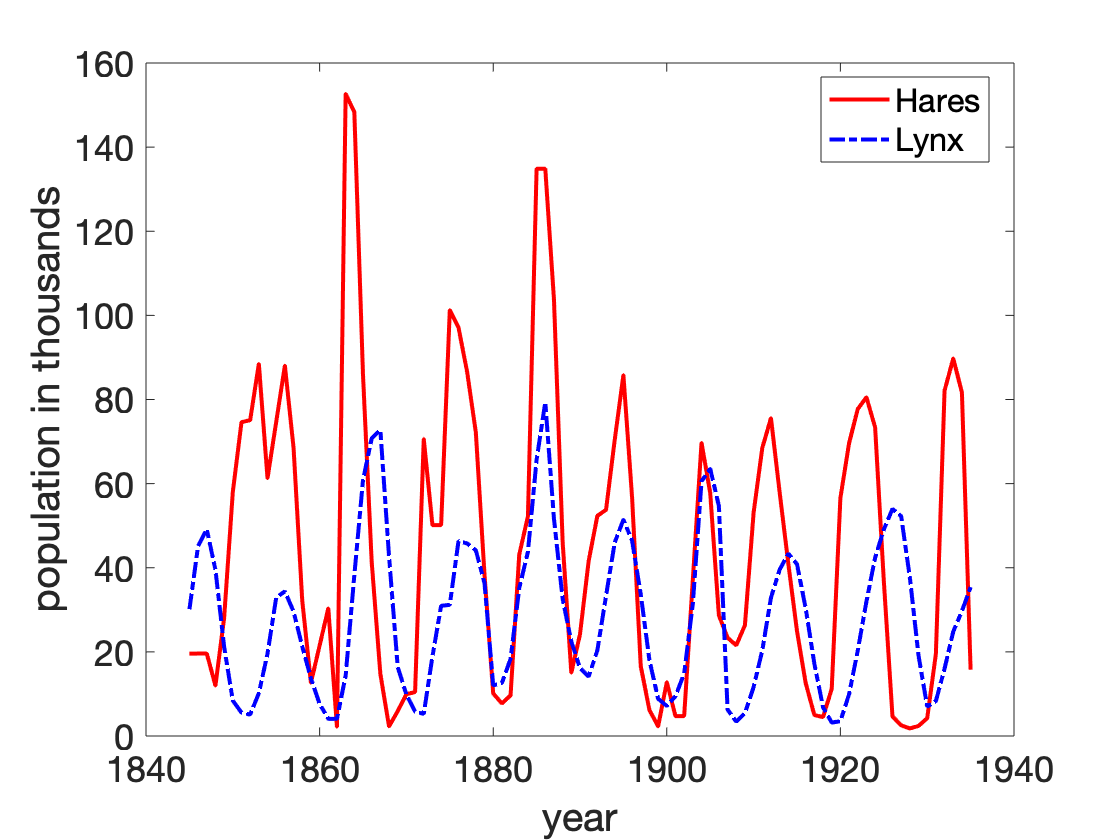
\includegraphics[width=15cm]{Model_Setup_Images/HaresLynxData.png}
    \caption{Hare-Lynx populations (in thousands) as determined by the pelt records of the Hudson Bay Company from 1845-1935. Note the oscillations between the populations, the hallmark of the Lotka-Volterra model.}
    \label{fig:0prob}
\end{figure}

\paragraph{Quantities of Interest} \label{section:LV_params}
All model parameters: $\alpha, \beta, \gamma, \delta$, are considered to be unknown. This makes them quantities of interest for estimation through MCMC, PSO, and Kalman Filtering. Additionally, an amount of noise exists within the data. The approach to account for this noise during paramterization is different between the parameterization techniques. In MCMC, noise is estimated iteratively as is detailed in Section \ref{Metropolis_MCMC}. In Kalman Filters, an estimate for the amount of Gaussian noise is made prior to the filtering process (detailed in Section \ref{noise_UKF}). Alternatively, in PSO we seek to estimate the amount of noise in the data \emph{during} the parameterization routine. This is done by treating the variance of noise for each species as an additional parameter: $\sigma^{2}_{H}$ and $\sigma^{2}_{L}$, for hares and lynx respectively. This assumes that the noise, $\epsilon$, within the two populations is independent. $\sigma^{2}$ represents the variance of this noise, assuming Gaussian noise centered around 0,
\begin{center}
$\epsilon_{h}\sim\mathcal{N}(0,\sigma_{h}^{2})$\\
$\epsilon_{l}\sim\mathcal{N}(0,\sigma_{l}^{2})$
\end{center}
In total, six parameters were estimated for in PSO, and four in both MCMC and Kalman Filtering. Denoting the parameter set by $\theta$,
$$\theta = [\alpha, \beta, \gamma, \delta, \sigma_{H}^{2}, \sigma_{L}^{2}]$$ for PSO, and $$\theta = [\alpha, \beta, \gamma, \delta]$$ for MCMC and the UKF.

\paragraph{Initial parameter guess} \label{section:LV_initParams}
In our implementations, MCMC and Kalman filters both require a user-defined initial guess for the values of the parameters. Notably, our implementation of PSO did not require a user-defined guess, but did require bounds to be defined for parameter values as discussed in Section \ref{param_bounds} . The same bounds were required for MCMC.
\par An initial parameter guess provides MCMC and the UKF a point from which to start their estimation. In practice, these initial parameters can be decided using a variety of means. However, a better initial parameter guess causes faster convergence to the ideal parameters determined by each algorithm.
Based on other parameterization work done on the Hudson Bay Company data set \cite{predpreyHudsonBay}, we initially guessed values $\alpha = \gamma = 0.7$ and $\beta = \delta = 0.1$, though we had no reference for the viability of these parameters. 
\par Due to our uncertainty, this guess was then improved by a running a preliminary \emph{unconstrained nonlinear optimization} routine with MATLAB's default \texttt{fmincon} (documentation found \textit{\href{https://www.mathworks.com/help/optim/ug/fmincon.html}{here}}) \cite{MATLAB:2020b}. Unconstrained nonlinear optimization is a common, fast, and relatively simple technique for parameter fitting \cite{Simunek2002nonlinearfitting} \cite{optimizationparamest_ppt}. By reducing the sum-of-squares difference between the model output and the data to a desired tolerance, a 'best-fit' set of parameters is chosen. While \texttt{fmincon} provides a good preliminary parameter estimate, MCMC and Kalman Filtering can be used to tune these parameters further, potentially resulting in a better fit. The resultant parameter set $\theta_{min}$ for MCMC and the UKF is 
\begin{center}
    $\theta_{min} = [0.625, 0.190, 0.661, 0.0468]$
\end{center}. 
This was taken to be the initial parameter guess.

\paragraph{Parameter bounds} \label{param_bounds}
Upper and lower bounds for the values of each parameter needed to be defined for both MCMC and PSO. In the general case, these bounds can be informed by reasonable, physical limits on the parameters (i.e. parameter $x$ must be non-negative), however when this information is not available, parameters are commonly let to vary a certain percentage above and below their initial value. Using the initial parameter guess for MCMC, values were allowed to range $\pm 100\%$. For the $\sigma_{H}^{2}$ and $\sigma_{L}^{2}$ values required by PSO but left undefined by $\theta_{min}$, ranges were defined using initial estimates for the variances. Residuals between the data and the model predictions solved using $\theta_{min}$ as defined above were found. Then, variances of these residuals was calculated to give
$${\sigma_{H}^{2}}_{initial} = 1487.277$$
$${\sigma_{L}^{2}}_{initial}  = 268.840$$
These values, like those in $\theta_{min}$, were also allowed to vary $\pm 100\%$, defining the upper and lower bounds.

\subsubsection{Type 1 Diabetes Model} \label{Type1_Diabetes_System}
Contemporary research is being done to model Type 1 diabetes (T1D) with dynamical systems. To demonstrate the utility of MCMC, PSO, and Kalman Filtering for parameter estimation in a realistic research context, one such model is examined.
\par Type 1 diabetes is an autoimmune disease characterized by the inability to regulate blood glucose, leading to chronically elevated glucose levels. These elevated glucose levels are a result of abnormal immune attacks on insulin-producing $\beta$-cells within the pancreas. Cells in the body respond to insulin by absorbing glucose from the blood, thus lowering blood glucose levels. Therefore, when these $\beta$-cells are damaged, and normal insulin production is disrupted, blood glucose rises to exceed healthy levels. 
\par One is genetically predisposed for Type 1 diabetes, however onset of the disease is theorized to be determined by the immune system's ability to respond to early structural changes in the pancreas, known as the \emph{apoptotic wave}. The apoptotic wave occurs in mammals during weaning when there are high rates of pancreatic $\beta$-cell apoptosis (natural, controlled cell death). As described above, the apoptosis of $\beta$-cells causes glucose levels to rise. Put simply, if blood glucose is able to return to healthy levels after this wave, diabetes onset does not occur. Likewise, if it is not, diabetes onset occurs, and chronically elevated glucose levels follow. The cellular mechanics of this onset are complex and largely uncertain, but hypothetical onset can be modeled with a dynamical system \cite{shtylla2019mathematical}.
\par Shtylla et al. details a single compartment model that models macrophage, immune cell, and dendritic cell populations within the pancreas, as well as blood insulin and glucose levels for genetically-engineered non-obese diabetic (NOD) mice. The 12-equation nonlinear ODE model includes 53 biologically-driven parameters, such as the volume of blood in the pancreas, the clearance rate of various macrophages, and the basal rate of glucose production, to name a few \cite{shtylla2019mathematical}. A description of these parameters and the equations of the model are included in Appendix A. In previous work, parameter values were estimated from biological literature and altered experimentally to resemble average system behavior seen in collected data, however the model was not parameterized directly to observed data.

\begin{figure}[H]
    \centering
    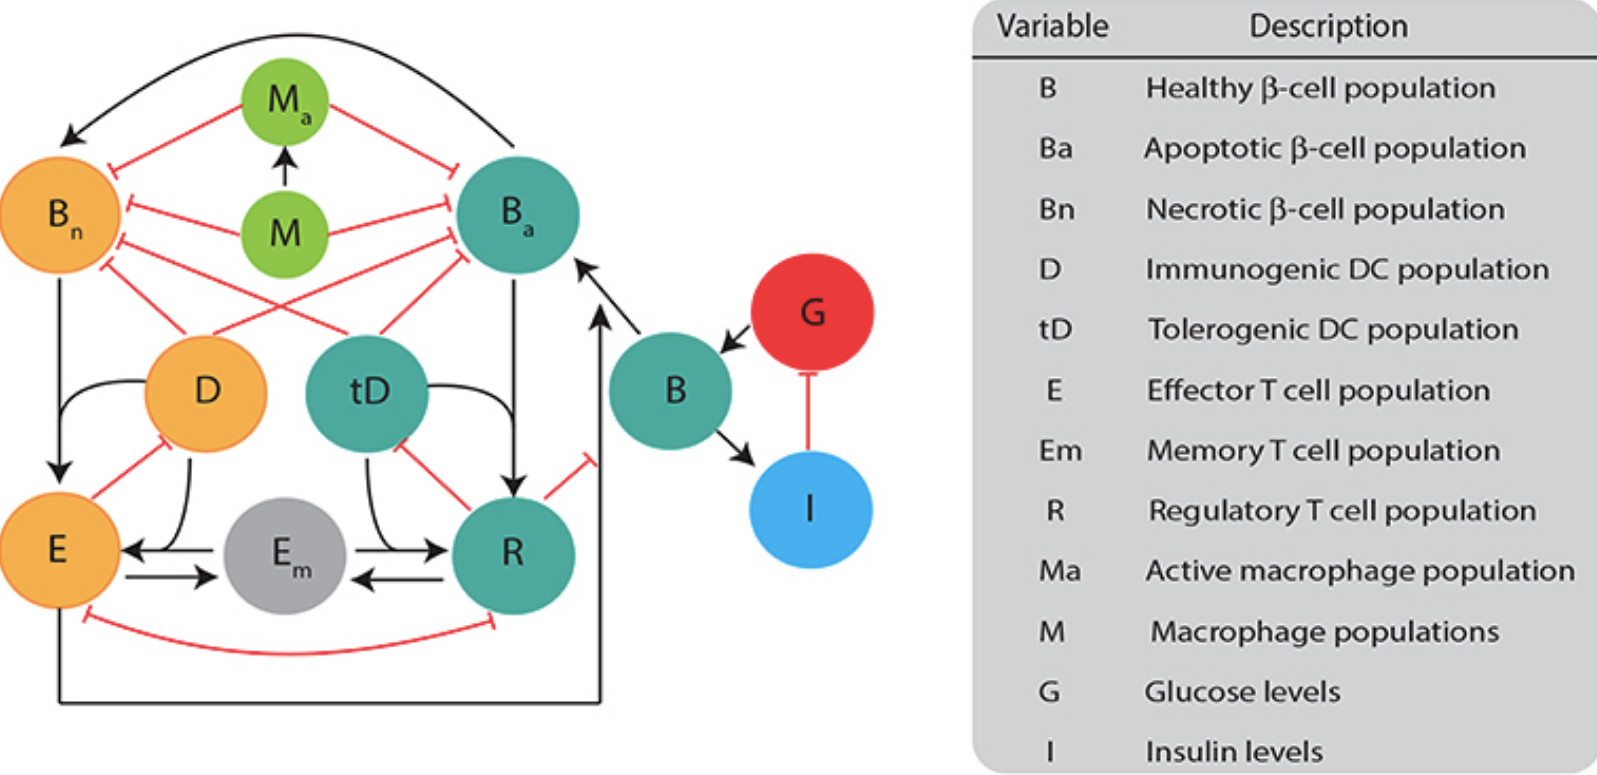
\includegraphics[width=15cm]{Model_Setup_Images/T1Dflowdiag.png}
    \caption{Flow diagram of T1D model in use, taken from Shtylla et al. 2019. As per Shtylla et al., "$\beta-$cell populations are split into three categories: healthy population ($B$), apoptotic cells ($B_{a}$), and necrotic cells ($B_{n}$). Healthy $\beta-$cells are involved in glucose ($G$) and insulin ($I$) regulation, whereas the dying $\beta-$cells (apoptotic and necrotic) interact with immune cells. Dendritic cells are split into two categories: immunogenic DC ($D$) and tolerogenic DC ($tD$) based on their ability to engage an immunogenic or tolerogenic T cell response. DCs in our model are assigned into a particular category once they engulf either apoptotic or necrotic $\beta-$cells. Macrophages can either be in an activated ($M_{a}$) or non activated form ($M$) based on their capacity to engulf $\beta-$cells. T cells are split into: regulatory T ($R$), effector T ($E$), or memory T ($E_{m}$). All populations are measured in cells ml−1 except for $B$ (mg), $G$ (mg/dl), and $I$ ($\mu$U)." \cite{shtylla2019mathematical}}
    \label{fig:flowdiag}
\end{figure}

\paragraph{Data}
While the Lotka-Volterra model functions on a population-level, data provided for the T1D model represents the system for a single mouse. In order to gain insights into the behavior of T1D in both individuals and on a population-level, the observed data used was manipulated to represent the cohort in its entirety. 

\subparagraph{Individual data} \label{section:T1D_individual_data}
Glucose data was measured in a cohort of 11 diabetic NOD mice by Li et al. 2009 \cite{Lietal2009}. In comparison to the 11 other quantities given by the Shtylla et al. model, glucose is easily measurable and a common quantity to keep track of in NOD mice \cite{Mathewsetal2015}. Glucose is also the metric used to diagnose and manage diabetes. Based on biological literature, Type 1 diabetes in NOD mice is diagnosed as having onset at a blood glucose level above 250 mg/dl \cite{Mathewsetal2015}.
\par In this data set and others of the same variety, there appear to be two distinct mouse behaviors: an \emph{acute} rise in glucose prior to onset, and a \emph{progressive} climb. Mice are classified visually and separated by this behavior \cite{Mathewsetal2015}. In the Li et al. data set, 9 mice were classified as acute and 2 as progressive. Our analysis focuses on the 9 acute mice, the raw data for which are included in Appendix \ref{general_appendix}.

\begin{figure}[H]
    \centering
    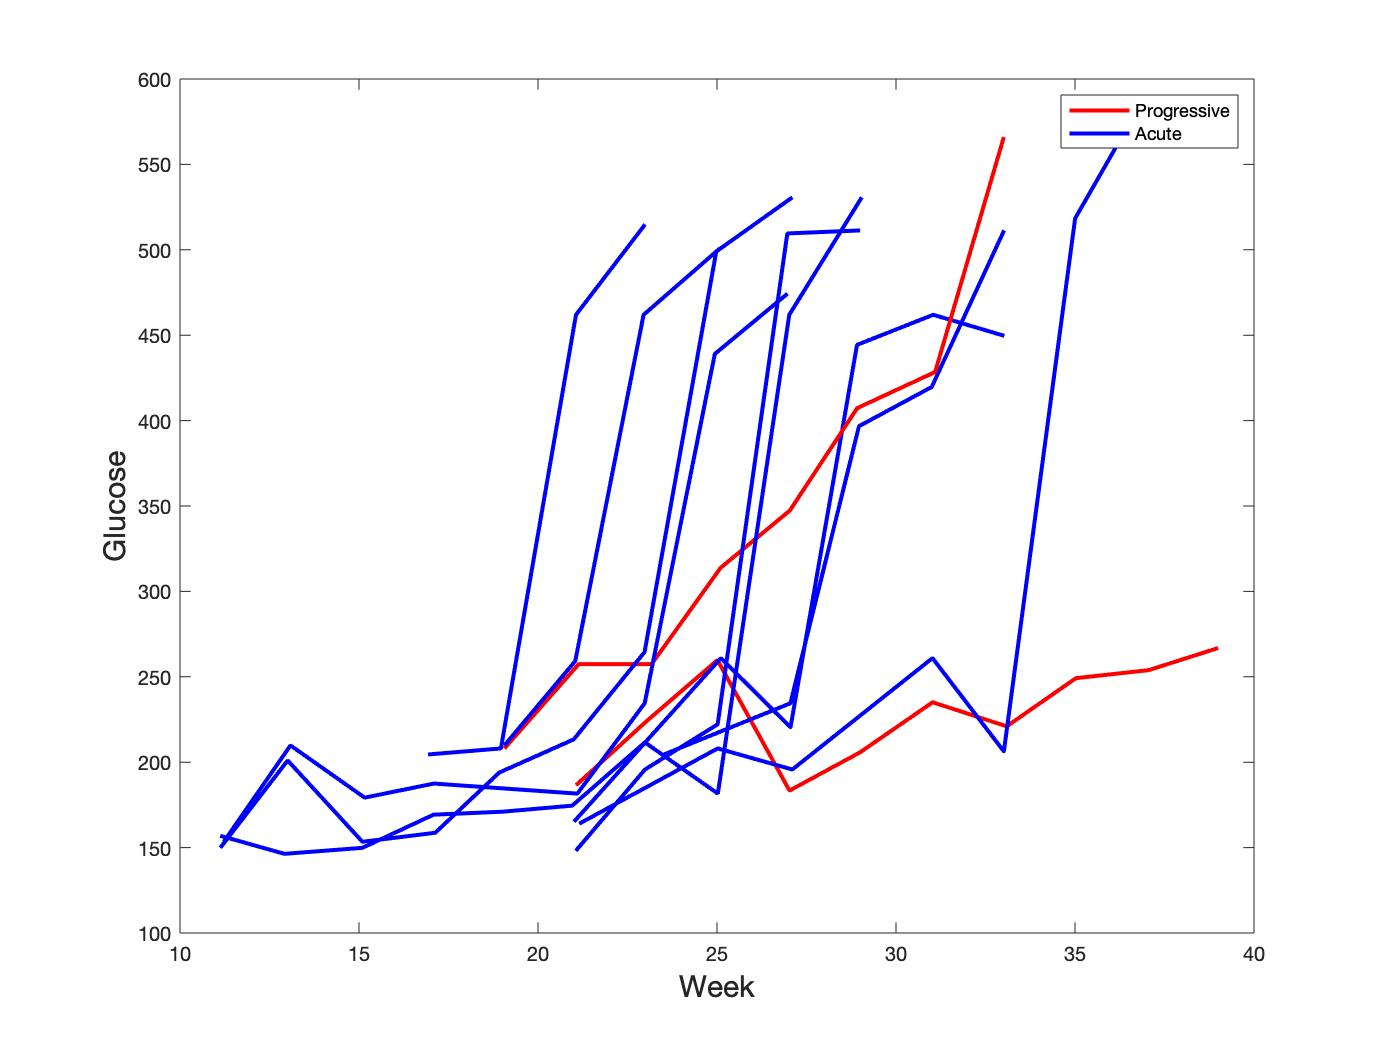
\includegraphics[width=15cm]{Model_Setup_Images/AcuteVersusProgressive.jpg}
    \caption{Glucose levels of the cohort of 11 NOD mice from Li et al.. The 2 mice that experience a progressive rise to diabetes onset are highlighted in red, while the 9 mice experiencing an acute form of onset are in blue.}
    \label{fig:1prob}
\end{figure}

\par In examining the data set itself, measurements are taken at inconsistent time points starting several weeks into each mouse's life. Time was measured in weeks as a decimal to include accuracy down to the time of day when the measurement was taken. On average, measurement started at week 30.47, and measurements were taken every 2.15 weeks. There was also not a consistent number of data points for each mouse in the cohort. Ranging from 4 to 11, the mean number of data points was 6.91. In order to make these somewhat sparse, inconsistently spaced data compatible with the dynamical system, they had to be converted to days. This was simply done by multiplying the associated week value by 7.

\subparagraph{Population-level data} \label{section:T1D_population_data}
We seek to estimate general parameters for diabetes onset in NOD mice, in addition to estimating parameters in a \emph{single} NOD mouse. As addressed within the descriptions of techniques themselves, the different parameterization techniques function differently to fit these population-level parameters. During our experimentation with different data sets, we found that Kalman Filters functioned best with individual mouse data sets due to the way in which the algorithms deal with the noise of the system and data. We also found that MCMC techniques tended to work better with the averaged data, likely due to the fact that MCMC is less concerned with error noise in the data. Thus, as will be explicitly explained in subsequent sections, the Kalman Filters use results from fitting each mouse individually to estimate population parameters and MCMC uses a population-level data set. PSO can use both approaches.
\par To construct a population-level data set from individuals' data, taking a point-by-point average is an intuitive, common method. However, this was avoided for the Li et al. data set. If averaged, the shape of the glucose curves would largely be lost due the staggering of diabetes onset times in the mouse population. Representing an average mouse would not be well-accomplished with this strategy. Instead, we developed a method to align each individual's glucose curve in time and then average all nine curves to preserve shape. 
\par While not ideal for larger data sets, our main approach was done by hand. We were most interested in the capturing the overall shape of the acute mice onset curve: the slow increase of glucose and the sudden spike indicating diabetes onset. Our approach relies on averaging both the glucose measurements and time spans of each mouse. Generally, we sought to align the 9 mice at the point immediately before the large spike in glucose that denoted onset (typically the 3rd or 4th point from the end), here we will name them \emph{pivot points}. This conserves the shape of the onset curve. \textbf{Figure 
\ref{fig:2prob}} highlights the pivot points within the acute Li et al data.
\begin{figure}[H]
    \centering
    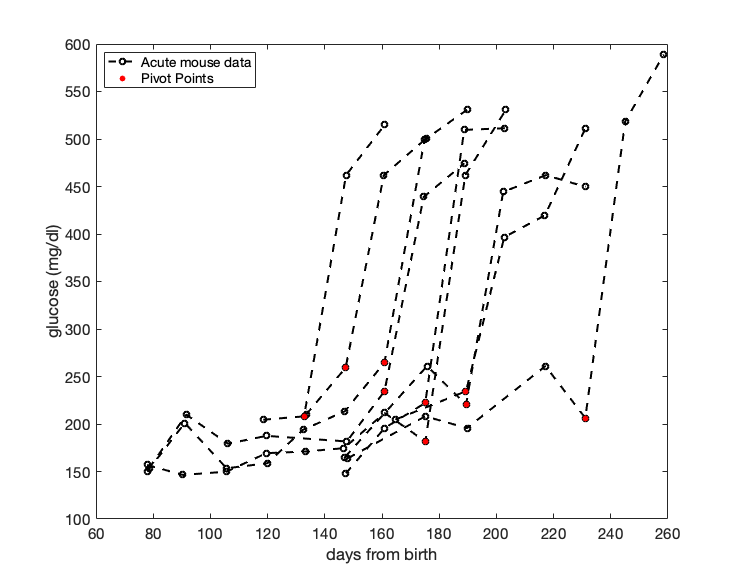
\includegraphics[width=15cm]{Model_Setup_Images/acute_pivotPoints.png}
    \caption{Diagram illustrating the process of determining glucose pivot points for 9 acute mice. Pivot points are indicated in red.}
    \label{fig:2prob}
\end{figure}
\par We began by discretizing the data: by creating an uniformly spaced time span incremented week by week, we could align the data points by absolute week of measurement, leaving weeks where mice were not measured blank. This was done in discrete, whole weeks. In determining which week to which to align each data point, we rounded weeks in the data set to the nearest whole number. For example, a measurement with the time 36.932 was aligned with the 37 week mark, while a time of 27.104 was aligned with the 27 week mark. \textbf{Figure \ref{fig:3prob}} shows this process for Mouse 6.
\begin{figure}[H]
    \centering
    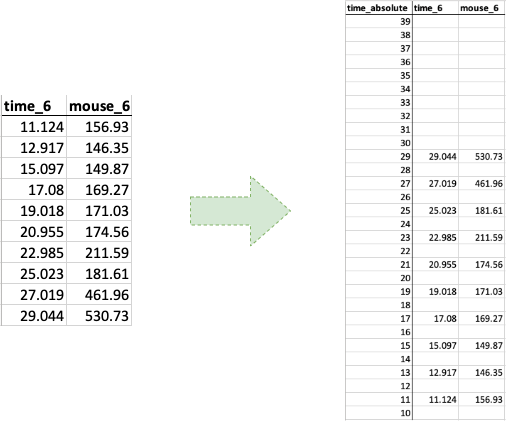
\includegraphics[width=15cm]{MCMC_figs/lietal_avg_diagram.png}
    \caption{Diagram illustrating the process of spacing Mouse 6 data within the 10-38 week time span. Using rounded times, Mouse 6 glucose measurements were spaced in an Excel sheet within the 10-38 week time span. The cells on the left show the original raw data with original time points and the cells on the right show how the original data is spaced within the prescribed 10-38 week time span.}
    \label{fig:3prob}
\end{figure}
The time series then needed to be shifted to align their pivot points before an average could be taken. This shifting simply involved the vertical movement of the time series in the spreadsheet, however the aligned curves must placed at some time along the $x$-axis. Shifting the data removes information about what this time should be. To define the time of pivot, we determined the average time of pivot across the population according to the data, and placed the pivot point accordingly. Times of the other data points were adjusted to maintain the correct spacing. Then, both the nondiscretized time values and the glucose values could be averaged and rounded to 3 significant figures to construct a data set representing the population: that of an average mouse. This process is diagrammed for Mouse 6 in \textbf{Figure \ref{fig:3prob}}. 
\par Lastly, each week value was multiplied by 7 to convert the timescale from weeks to days. The Shtylla et al. model uses days as its time scale, so this conversion makes the data set and the model compatible.
\par \textbf{Figure \ref{fig:4prob}} shows the plot obtained after the shifting and averaging process. As pictured, the sharp spike in glucose observed on the individual level is conserved, avoiding the issues encountered when taking averages. This was taken to be the population-level data set. 
\begin{figure}[H]
    \centering
    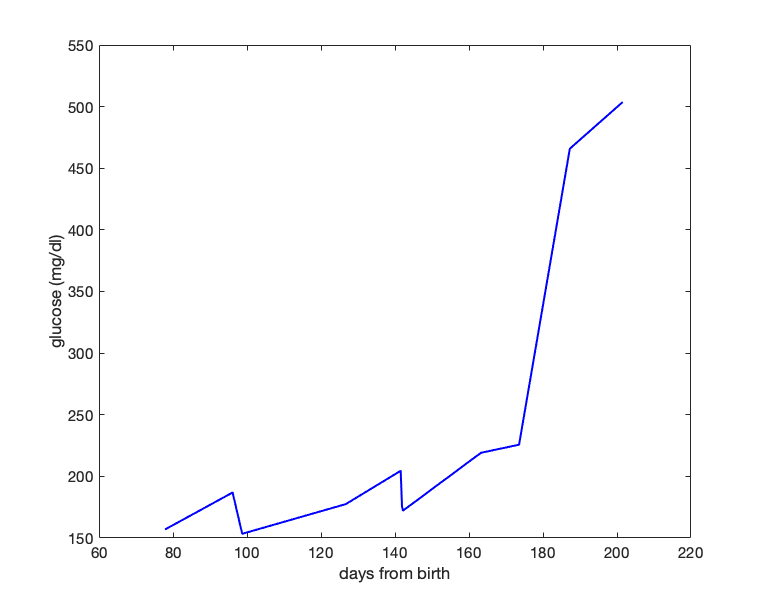
\includegraphics[width=15cm]{Model_Setup_Images/avg_raw_plot.png}
    \caption{Plot of the averaged and shifted acute mouse data. Constructed from 9 individual NOD mice, this was taken to represent the population-level data set.}
    \label{fig:4prob}
\end{figure}
\paragraph{Quantities of Interest}
There are 53 biologically-informed values built into the model, however 12 function as conversion rates, or otherwise known quantities \cite{shtylla2019mathematical}. Since these are known to be constant and pre-defined, they are not included in $\theta$. The remaining 41 values are treated as variable within the system and are quantities of interest for parameter estimation. For more information see Appendix \ref{general_appendix}.
\par To minimize computation and incorporate more certainty about parameters in the system, subsets of these 41 parameters were estimated while other parameters were held relatively constant. By letting some parameters remain relatively constant, we tell our system that we are fairly confident that their values are correct. However, the values are still allows to change in very small ways; 1 percent of their original range. This was done to account for correlations between the parameters. As of yet, sensitivity analysis has not been done to identify correlated parameters, so this step was taken to encourage the natural behavior of related parameters, even within the limited system.
\par These subsets were chosen experimentally. Only one of the tested subsets proved significant, referred to as the \emph{notable parameter subset}. This subset allowed for enough flexibility to find a relatively good fit to data, unlike others tested.
\subparagraph{Notable parameter subset} \label{section:NotableParameterSubset}
The notable parameter subset is composed primarily of 'active' parameters according to the Kalman Filter. 'Active' describes a greater than 1 percent change from the baseline to the fitted value for each parameter when the UKF was run on all the parameters. Upon inspection of the results from Kalman Filtering, few parameters moved beyond this threshold, so these parameters were marked as significant. Seven parameters were marked as active: $G_{I}, S_{I}, \mu_{E}, \mu_{R}, e_{1}, e_{2},$ and $\delta_{B}$.
\par In addition to the active parameters, three other parameters were added to the notable set: $\eta, \alpha_{\eta}, and \beta_{\eta}$, referred to as the $\eta$ parameters. Simply put, these parameters relate to the effectiveness of T-cells at eliminating insulin-producing $\beta$-cells. This heavily impacts the time of diabetes onset, and thus manipulating these parameters allows for horizontal shifting of the fit. While the active parameters influence the shape of the glucose spike more, these $\eta$ parameters allow for greater flexibility in the onset time. Shape and position are the main indicators of fit, and this notable parameter set does a sufficient job of addressing both while lessening computation and building more certainty about parameters within the system. 
\par This subset was required only by MCMC due the need to have more data points than parameters. However, for comparison purposes, the subset was also run in PSO. 

\paragraph{Initial parameter guess}
As parameterization of the model using the methods in this paper is intended to improve upon the findings in Shtylla et al., the biologically estimated parameters and initial conditions from Shtylla et al. were used as an initial guess $\theta$ for the parameters for each technique \cite{shtylla2019mathematical}. 

\subsection{Comparison Methodology} \label{Methodology}
In order to evaluate and compare the effectiveness of each parameterization technique, a method needed to be devised to quantify a model's goodness of fit to a data set. Because the goal of each parameterization technique is to produce system predictions that are close to observed data, this metric needs to measure the distance between the model and the data. Root Mean Squared error (RMSE) was chosen as this metric to quantify the mean residual between the model and the data set at one data point. 
\par RMSE quantifies the standard deviation of residuals, or prediction errors. The prediction error is the distance between the model prediction and the observed data at each time point $t$. RMSE tells us how concentrated the original data points are around our prediction. This was thought to be a more useful technique than simply MSE, or mean squared error, due to the magnitude of the datapoints observed. For more information regarding RMSE see \textit{\href{https://statweb.stanford.edu/~susan/courses/s60/split/node60.html}{here}.}

\section{Markov Chain Monte Carlo Methods} \label{MCMC_SECT}
\subsection{Bayesian Techniques} \label{Bayesian_Techniques}
Bayesian inference is a powerful tool in parameter estimation for biological systems that begins with previously known information and updates a system using new, incoming data \cite{bayesian_param_inf}.  In particular, Bayesian inference techniques have been used to parameterize a variety of biological models and systems, \cite{bayesian_param_inf_ex1}, \cite{bayesian_param_inf_ex2}. In the following sections, we outline the basic mathematical concepts behind the Bayesian inference technique Markov Chain Monte Carlo (MCMC) method, introduce two specific implementations of MCMC methods, and parameterize two different biological nonlinear ODE systems.
\subsubsection{Bayesian Parameter Estimation}
Bayesian parameter estimation is a process of inferring a posterior probability density function (PDF) over a model's possible parameters given data, $D$, for some model, $M$ \cite{astrostats}. This PDF can be evaluated for a set of parameters, giving individual probabilities. Parameters of a system are treated as random variables and realized as $\theta = [p_1, p_2,...,p_n]$, where $p_i$ is a parameter of a modeling system. They follow distributions that incorporate both \emph{a priori} knowledge such as mathematical models or theory, about their values, as well as information obtained from data collection. When estimating a system's parameters, $\theta$, a variety of Bayesian techniques can serve to find a posterior density, the post-parameterization distribution of parameter values based on sampled data and a given model \cite{bayesprior}. This technique relies on Bayes' Theorem which is defined as follows:
\begin{equation} \label{eq:1mcmc}
P(\theta | D, M) = \frac{P(D|\theta, M)P(\theta|M)}{P(D|M)}
\end{equation}
where $\theta$ denotes a set of parameters. $P(D|\theta, M)$ is referred to as the \emph{likelihood} and denotes the probability of the data given the current parameters and model \cite{astrostats}. $P(\theta|M)$, or the \emph{prior}, gives the probability of a set of parameters for a given model, before the data can inform the system \cite{astrostats}. Finally, the denominator $P(D|M)$ is known as the \emph{evidence} \cite{astrostats}. The evidence (also called the normalization constant of the posterior probability) does not depend on $\theta$. In mathematical terms, because our posterior, $P(\theta|D,M)$ is a \textit{density function}, we need the right hand side of \textbf{Eq. \ref{eq:1mcmc}} to integrate to 1 (and avoid a situation of dividing by 0) \cite{bayesprior}, without the normalization constant, this is not possible. However, it is often difficult to calculate $P(D|M)$ (as the integral may not be closed-form) and many mathematicians choose to work with a variation of Bayes' Theorem:
\begin{equation} \label{eq:2mcmc}
P(\theta|D,M) \propto P(D|\theta,M)P(\theta|M)
\end{equation}
as it is possible to compute the priors and likelihoods. We work initially with \textbf{Eq. \ref{eq:1mcmc}} in this tutorial, but 
through derivations shown in Section \ref{The_Likelihood_Function}, we arrive at Eq. \ref{eq:2mcmc}. Thus the quality of posterior estimation relies heavily on choices of the likelihood and prior which are informed by \textit{a priori} knowledge.
\paragraph{The Curse of Dimensionality}
Many models have a significant number of parameters which leads to a high-dimensional parameter space, and thus a high dimensional posterior PDF. The best-fit set of of parameters for the model would be located at the peak of this multi-dimensional PDF, as these are, by definition the parameters located at the highest probability of the overall modeling system. 
\par Due to the unknown shape of the PDF, this maximum likelihood cannot be found analytically. Additionally, searching for it directly (discrete calculations for example) poses a challenge. While sufficiently sampling a one-dimensional PDF might require $N$ samples, sufficiently sampling a two-dimensional PDF requires building a grid of $N^{2}$ samples, and a $j$-dimensional PDF consequently requires a hypercube of $N^{j}$ samples. This exponential increase is known as the \emph{curse of dimensionality} \cite{astrostats}. Evaluating the posterior PDF for $N^{j}$ samples is computationally infeasible. Moreover, the probability of the majority of the these coordinates is very small adding to the computational difficulty. To overcome the curse of dimensionality, we instead look to \emph{sample} the posterior PDF directly. In effect, these samples simulate the distribution itself and feasible predicted values of parameters can be extracted from the simulation. One class of methods for such sampling is known as Markov Chain Monte Carlo methods, or MCMC methods. We will explore two MCMC algorithms and parameterize both the Lotka-Volterra and Type 1 Diabetes mathematical models. 

\subsection{Markov Chain Monte Carlo Sampling} \label{Markov_Chain_Monte_Carlo_Sampling}
Markov Chain Monte Carlo methods are used to describe posterior distributions when there is incomplete knowledge of the distribution's properties (such as its mean or variance) \cite{MLEvsBayes_powerpoint}. 
\par The idea driving MCMC is that of \textbf{Monte Carlo} methods. We are working in probabilities (via Bayes' Theorem), thus we rely on the probabilistic Monte Carlo method in which we observe quantities chosen to simulate the physical or biological processes of our model and infer a solution from their behavior \cite{montecarlo}. In the context of ODE system parameterization, we draw samples of parameters from an arbitrary probability density using random numbers drawn from a simpler distribution \cite{astrostats} and infer posterior probabilities. MCMC uses a \textbf{Markov Chain} to perform \emph{rejection sampling} - that is, given a proposal distribution (a distribution of parameter values that we draw candidates from), we draw samples and penalize with an acceptance criteria (a ratio). Briefly, a Markov chain is a process in which we move among a set of elements $X$ according to a specified probability. Beginning at element $x_1 \in X$ we move to $x_2 \in X$ according to a probability distribution $P(x_1, *)$ which depends only on $x_1$ \cite{markovchains}. We use an asterisk to signify a multitude of possible probabilistic rules that could be applied that depend on the specifics of a model. For example, in a very simple system, let us say that we have a sequence of values $[0,1,...10]$. We might start at a value 0 and move with probability $\frac{1}{3}$ to an even value, move with probability $\frac{1}{3}$ to an odd value, and stay at 0 with probability $\frac{1}{3}$. The Markov ``chain" refers to the order and values of elements in $X$ that we have visited (or collected).
The Markovian aspect of this algorithm establishes a random walk over the parameter space such that we can preferentially sample regions of high probability. Furthermore, since each `step' along this walk is only dependent on the previous, we classify the MCMC as a first-order Markovian process \cite{firstorderMarkovian}. 

\par The umbrella of MCMC methods is broad, but here we introduce implementations of the simplest algorithm, Metropolis MCMC, as well as a method derived from Metropolis, delayed rejection adaptive Metropolis (DRAM) MCMC. We find that looking at these two methods of sampling gives the reader a good idea of the range of capabilities that MCMC can provide for parameterization. Metropolis MCMC provides the most basic search in parameter space and is likely to find local probabilistic maxima (rather than global maxima). That is, due to the algorithm's search method, Metropolis MCMC will tend to settle in an area of parameter space with high probability according to the model and rarely move into areas of lower probability. This is detailed in Section \ref{Metropolis_MCMC}. DRAM on the hand, is more likely to find global probabilistic maxima as the algorithm is able to search and sample lower probability parameter space.

\subsubsection{Defining Bayes' Theorem} 
Bayes' Theorem is the underlying framework in the MCMC algorithm of accepting and rejecting samples. In this section we further specify elements of Bayes' Theorem in terms of a mathematical model and its parameters following a tutorial in \cite{astrostats}. We introduce two new concepts: the proposal distribution from which we draw parameter samples and the acceptance criteria which we use to accept and reject candidates.
\paragraph{The Prior Distribution} \label{section:ThePriorDistribution} The \emph{prior function} is the uncertainty that we have about a specific set of parameters \emph{before} we observe any data and informs us how likely we are to have sampled that set of parameters \cite{astrostats}. We can specify the prior distribution based on \textit{a priori} knowledge about our biological system \cite{bayesprior}. For example, if we know from previous experimentation the range of variation that we expect a parameter to exhibit, we can constrain the parameter candidates that we draw accordingly. However, when we know nothing about our parameter values, we initialize an uninformative prior distribution - a uniform distribution \cite{astrostats}:
\begin{center} \label{eq:3mcmc}
\begin{align}
  P(\theta|M) = \left\{ \begin{array}{cc} 
                \frac{1}{b-a} & \hspace{5mm} a \leq \theta \leq b \\
                0 & \hspace{5mm} otherwise \\
                \end{array} \right.
\end{align}
\end{center}
It is important to note that we must know enough about the parameters of the system in order to make a decision about the bounds of the uniform distribution. When implementing a prior function, we specify the range of the distribution such that the values of $\theta$ will always be constrained between the bounds. For example, in a biological system we could say that it is biologically infeasible for a particular parameter value to be negative. In effect, we do not want our prior function to be 0 because in computing the acceptance ratio (discussed in \ref{The_Acceptance_Criteria}), we will encounter a situation of dividing by 0. Consequently, the prior distribution becomes
\begin{equation} \label{eq:4mcmc}
P(\theta|M) = \frac{1}{b-a}
\end{equation}
That is for any values of $\theta$ our prior distribution will be never be 0. It is important to point out with this definition, we have specified the same uniform interval, $[a, b]$, for all parameter sets. Now what does this mean in the context of parameterization and why would we choose to do this? If we truly have no \emph{a priori} information about our model and its parameters, then we do not want to implement any bias when accepting and rejecting samples. In other words, we want each sample to be equally likely (in terms of being informed by the prior) and the uniform prior achieves this for us. 
\paragraph{The Likelihood Function} \label{The_Likelihood_Function} The \emph{likelihood function} represents the relationships between independent evaluations of a model (given specified parameters) and it informs us \emph{how} to accept samples of parameters from the specified proposal distribution. In a biological model, we would assume that there exists some amount of error, or noise, within the model itself. If we have $D = \{x_1,...,x_n; y_1,...,y_n\}$ with $n$ data points, then our model $M$ predicts values of $y$ to be
\begin{align} \label{eq:5mcmc}
y_1 = f(x_1) + \epsilon_1 \cdots y_n = f(x_n) + \epsilon_n
\end{align}
where $f(x_i)$ is the evaluation of the ODE system and $\epsilon_i$ is our system noise \cite{astrostats}. The most general assumption we can make is that the noise is an independent and identically distributed (every random variable has the same distribution and each is independent of the others) Gaussian distribution with a mean of 0 and a standard deviation $\sigma$. 
\par The distribution of the likelihood informs us how different evaluations of the model are distributed given varying parameter values \cite{smithCh8}. Thus, when we accept sampled parameter values, we will do so according to the likelihood function's distribution. Often, the likelihood is given as a normal distribution
\begin{equation} \label{eq:6mcmc}
    P(D|\theta, M) = \frac{1}{\sigma \sqrt{2\pi}} e^{-\frac{SS_{\theta}}{{2\sigma^2}}}
\end{equation}
where $SS_{\theta} = \sum_{i=1}^{n}[y_i - f_i(\theta)]^2$ is the sum of squares error between the predicted model and the original data and $\sigma$ refers to the standard deviation of the noise \cite{smithCh8} \cite{astrostats}.
\par It is important to note that $\sigma$ is often unknown. We may know that our system produces some noise, but we are not able to quantify it via a specific standard deviation. In this case, we can simply use an estimate for $\sigma$, denoted as $s$. There are a variety of ways to estimate $s$, however in practice, we use the following estimation
\begin{equation} \label{eq:7mcmc}
s^2 = \frac{SS_{\theta}}{n-p}
\end{equation}
where $n$ is the total number of data points, $p$ is the number of parameters and $SS_{\theta}$ is as defined above \cite{smithCh8}.
\paragraph{The Posterior Distribution} The \emph{posterior distribution} is the accumulation of samples in the chain that are accepted and to which a distribution can be fitted. Not only can we extract the PDF of a set of parameters, we can extract individual parameter PDFs \cite{astrostats}.
\paragraph{The Proposal Distribution} We now must introduce a new element that is not a part of Bayes' Theorem: the proposal distribution. This is the distribution from which we draw the values of our samples. If we have \textit{a priori} knowledge about our parameter space, we can specify our own distribution, but when no knowledge is available, a normal distribution is often assumed \cite{astrostats} \cite{bayesprior}. For certain MCMC algorithms, like the Metropolis MCMC, the proposal distribution must be symmetrical \cite{smithCh8}. A proposal distribution $J$ is considered symmetrical if $J(\theta^{*}|\theta^{k-1}) = J(\theta^{k-1}|\theta^{*})$, where $\theta^*$ is the proposed sample and $\theta^{k-1}$ is the current sample \cite{smithCh8}. In symmetric sampling, the order of selecting parameters does not matter; that is, the probability of moving from sample $a$ to sample $b$ is the same as moving from $b$ to $a$.
\par In order to get the best parameterization of our model, we want to establish a proposal distribution from which we believe we will be able to sample the best values for our model. In practice, it is common to initialize a multivariate Gaussian distribution \cite{astrostats} \cite{mcmcstatlib}. We can implement a covariance matrix to represent this proposal distribution. The coefficients of this matrix will represent the effect that perturbations of varying parameter values may have on the system \cite{sensitivity_matrices1}. In our Gaussian proposal scenario, we define the proposal 
\begin{equation} \label{eq:8mcmc}
V = J(\theta^*|\theta{k-1})
\end{equation}
where $J$ is defined as a Jacobian output matrix \cite{sensitivity_matrices1} \cite{smithCh8}. The proposal is distributed as $N(\theta^{k-1}, V_{cov})$ where $V_{cov}$ is the covariance matrix for $\theta$ \cite{smithCh8}. (Note that $V_{cov}$ must be positive definite.) In the \texttt{mcmcstat} library function \texttt{mcmcrun}, this covariance matrix is computed internally \cite{mcmcstatlib}.
\par One way to construct $V$ by hand is to use a sensitivity matrix. Briefly, this matrix is calculated by computing the Jacobian matrix of the derivatives of the parameters and the model. For a more in-depth calculation of $V$ we refer the reader to \cite{smithCh8} and \cite{sensitivity_matrices1}.
\paragraph{The Acceptance Criteria} \label{The_Acceptance_Criteria} As we pointed out before, the acceptance criteria is the element of MCMC sampling that allows the algorithm to accept and reject proposed samples in the Markov chain. We want to discriminate between samples of parameters based on their probabilities, only accepting the best (the most likely according to our likelihood, prior, and proposal functions) sets. To do this, we accept parameter sets according to a ratio, $\alpha$, which is a direct application of Bayes' Theorem \cite{astrostats}. While $\alpha$ may differ slightly according to the specific MCMC algorithm begin implemented, a basic ratio compares the posteriors of a proposed set of parameters ($\theta^*$) with the last accepted set of parameters ($\theta^{k-1}$) as follows:
\begin{equation} \label{eq:9mcmc}
\alpha = min(1, \frac{P(\theta^*|D, M)}{P(\theta^{k-1}|D,M)}) = min(1, \frac{\frac{P(D|\theta^*, M)P(\theta^*|M)}{P(D|M)}}{\frac{P(D|\theta^{k-1}, M)P(\theta^{k-1}|M)}{P(D|M)}}) = min(1, \frac{P(D|\theta^*, M)P(\theta^*|M)}{P(D|\theta^{k-1}, M)P(\theta^{k-1}|M)})
\end{equation}
Notice that the \emph{evidence} term of Bayes' Theorem (the denominator) cancels out. Intuitively, this cancellation makes sense because we are only interested in comparing the impact of different parameter sets on the model, but the evidence does not depend on the parameters at all. If 
\begin{equation} \label{eq:10mcmc}
P(D|\theta^*, M)P(\theta^*|M) \geq P(D|\theta^{k-1}, M)P(\theta^{k-1}|M)
\end{equation}
we accept $\theta^*$ with a probability of 1. If this is not the case, we still want to accept $\theta^*$ with some probability, the ratio between products of likelihoods and priors \cite{astrostats}. We never want to perform an immediate rejection of any parameter set because we assume that we will find a majority of our ``best" parameter values given the prior and likelihood functions that we have chosen. Thus, while a candidate may not be the best parameter set according to $\alpha$, it can still inform our posterior distribution. So, we want some probability of accepting any sampled parameter set. In addition, if we outright reject any candidate that does not meet the acceptance criterion, we run the risk of getting stuck in a very small range of values to sample from since our next parameter candidate depends directly on the previously sampled (and accepted) parameter set due to the Markovian process of the algorithm.
\par To get a better understanding of how $\alpha$ is constructed, let's use our Gaussian likelihood and uniform prior on the interval $[a, b]$. The acceptance criterion becomes
\begin{equation} \label{eq:11mcmc}
\alpha = min(1, \frac{P(D|\theta^*, M)(\frac{1}{b-a})}{P(D|\theta^{k-1},M)(\frac{1}{b-a})}) = min(1, \frac{\frac{1}{\sigma \sqrt{2\pi}} \exp^{\frac{SS_{\theta^*}}{{2\sigma^2}}}}{\frac{1}{\sigma \sqrt{2\pi}} \exp^{\frac{SS_{\theta^{k-1}}}{{2\sigma^2}}}})
\end{equation}
which simplifies to
\begin{equation} \label{eq:12mcmc}
    \alpha = min(1, exp^{-[-SS_{\theta^*} - SS_{\theta^{k-1}}]/2\sigma^2}) \cite{mcmcstatlib}
\end{equation}
\paragraph{Overview} So how does sampling create a usable posterior distribution? Figure 1 illustrates the MCMC process.
\begin{figure}[H]
    \centering
    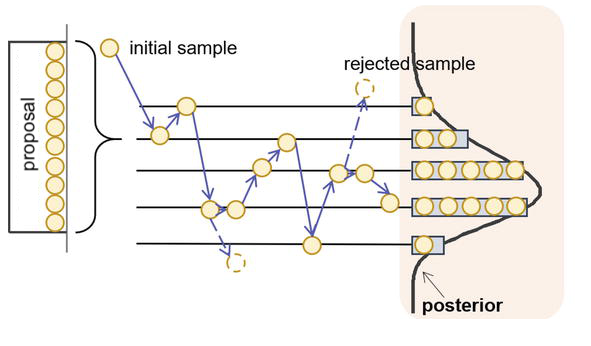
\includegraphics[width=15cm]{MCMC_figs/mcmc_procedure.png}
    \caption{Markov chain Monte Carlo sampling using random walk. Image adapted from \cite{mcmcFig} Figure 3.}
\end{figure}
We start with a general pool of potential parameter values - our proposal distribution. As we iterate through the chain, accepting and rejecting a samples - using the acceptance criterion, eventually we can fit our accepted samples to a distribution, the posterior distribution.
\subsection{Metropolis MCMC} \label{Metropolis_MCMC}
The single-chain Metropolis MCMC algorithm is one of the most basic and widely implemented MCMC methods. The simple acceptance-rejection method of sampling means that the Metropolis MCMC method tends to find local probabilistic maxima as once it has determined a high probability range of values within the parameter, it is unlikely to explore further away from that area. The Metropolis algorithm is a special case of another common MCMC algorithm, the Metropolis-Hastings algorithm \cite{metropolis1953}. The Metropolis algorithm requires a symmetric proposal distribution, whereas Metropolis-Hastings does not \cite{smithCh8}. Below, we outline the algorithm for the the Metropolis MCMC method.
\begin{tcolorbox} \label{alg:met}
\textbf{\underline{Metropolis MCMC Algorithm (with an uninformative prior)}} 
\begin{enumerate}
    \item Set number of samples to take, $N$ and determine a burn-in period, $k_b$
    \item \label{step:2met} Determine an initial parameter guess, $\theta^0 = argmin_\theta \sum_{i=1}^{n}[M_i - f_i(\theta)]^2]$

    \item Set $SS_{\theta^0} = \sum_{i = 1}^{n}[y_i - f_i(\theta^0)]^2$ (for initial likelihood, see \ref{The_Likelihood_Function})
    \item Compute an initial error variance estimate $s_0^2 = \frac{SS_{\theta^0}}{n-p}$ ($n = $ number of data points, $p = $ number of parameters)
    \item Construct proposal covariance matrix $V$
    \item \label{step:6met}For each iteration of the chain, $k = 1,...,N$ 
    \begin{enumerate}
        \item Sample $z \sim N(0,I_p)$ 
        \item Construct candidate $\theta^* = \theta^{k-1}+ Vz$
        \item Compute $SS_{\theta^*} = \sum_{i = 1}^{n}[y_i - f_i(\theta^*)]^2$ (for likelihood)
        \item Compute acceptance criterion
            \begin{center}
                $\alpha(\theta^* | \theta^{k-1}) = min(1, \frac{P(\theta^* |D, M)}{P(\theta^{k-1}|D, M})) = min(1, e^{-[SS_{\theta^*}-SS_{\theta^{k-1}}/2s_{k-1}^2]})$
            \end{center}
        \item Accept $\theta^*$ with probability 1 if $\alpha \geq 1$ and accept it with probability $\alpha$ if $\alpha < 1$.
        \begin{itemize}
            \item If $\theta^*$ is accepted
            \begin{center}
                $\theta^k = \theta^*$, $SS_{\theta^k} = SS_{\theta^*}$
            \end{center}
            \item Else
            \begin{center}
                $\theta^k = \theta^{k-1}$, $SS_{\theta^k} = SS_{\theta^{k-1}}$
            \end{center}
        \end{itemize}
        \item If $k > k_b$ collect $\theta^*$ in posterior matrix $P$, else discard.
        \item Update $s_k^2 = \frac{SS_{\theta^k}}{n-p}$
    \end{enumerate}
\end{enumerate}
\emph{Based on Smith (2014) Algorithm 8.5}
\end{tcolorbox}
\par We want to determine a number of samples to take, $N$ so that we can be sure that the resulting accepted parameter values approach the posterior distribution. Since we are sampling a parameter space via random-walk (since $\theta^*$ only relies on $\theta^{k-1}$), we want our algorithm to settle into an area of values that are highly likely to fit our model $M$. Thus, we want the chain to reach \emph{convergence} or a steady state. We can increase the likelihood of convergence occurring by performing \emph{burn-in} iterations ($k_b$) of the chain. That is, we sample according to the Metropolis algorithm, however we must discard the beginning of the chain. This allows the chain to explore the parameter space, determine local maxima, and increases the probability that when we collect samples, they will reflect our desired posterior. The burn-in period is a sliding scale and can be determined mathematically \cite{rafferty1992burnin}, however, in this tutorial we implement a burn-in of  $\sim 10\%$ of the total chain length as this is a common percentage of samples in the literature.
\par Note that in Step \ref{step:2met}, $\theta^0$ is found by minimizing the ODE model and extracting the parameter values. In practice we use the MATLAB \texttt{fmincon} function to do this. It should be noted that initial values of $\theta$ may be found in different ways, for instance if the user may specify values based on previous experimentation or calculation. In Step \ref{step:6met}a, we sample a normal value $z$ such that $z \sim N(0,I_p)$ where $I_p$ is an identity matrix of $p$-by-$p$ (the number of parameters) dimensions. Intuitively, $z$ is the random component of selecting a parameter set and is what makes each $\theta^*$ unique even if multiple $\theta^*$s are found using the same $\theta^{k-1}$. Since our $V \sim N$, $z$ must also be Gaussian. Note that in Step \ref{step:6met}b, we can see the Markovian influence as the candidate parameter is selected based on the previously accepted parameter set.

\subsubsection{Parameterizing Lotka-Volterra} Parameterizing a simple biological model using the Metropolis method is a good way to get familiar with the role of the elements of Bayes' Theorem and MCMC. Here we have parameterized the classic predator-prey model in MATLAB based on a tutorial in R originally intended for parameterizing a small non-linear ODE system \cite{mcmcstatlib}. It is important to note that MATLAB has its own implementation of the Metropolis MCMC method, \texttt{mhsample}. However, using this function requires an initialization routine similar to the one that we outline here. We are using the functions from the MATLAB \texttt{mcmcstat} library \cite{mcmcstatlib} and so we implement the components of the Metropolis MCMC method according to requirements of this algorithm. 
\par We consider 4 parameters in this model: $\theta = \{ \alpha, \: \beta,\: \delta,\: \gamma \}$ (full details of the Lotka-Volterra ODE model can be found in Section \ref{Lotka_Volterra_System}). We begin our parameter estimation by establishing an initial guess for our parameter values and their ranges (see \ref{section:LV_params} for details). As a general guide for creating our parameter ranges, we knew that our parameter values would never be negative. Through experimentation, we found that a good starting place would be to have a range of $\pm$ a reasonable percentage (at maximum 100$\%$) and to constrain the lower end of the range to 0. We settled on using a range of $\pm 10\%$ of our initial parameter values as this seemed to create a sufficient parameter space for sampling. We assume a Gaussian likelihood function in log (base e) form (Step 3). Due to the sum of squares calculation for the likelihood function (see Section \ref{The_Likelihood_Function}) we will be dealing with larger numbers (on the scale of 10e03 to 10e04). Thus, the natural log form is chosen for computational ease as we are able to compute sums rather than products and prevent exponential increase in values. The sum of squares between the model given parameter values and the original data is thus
\begin{equation} \label{eq:13mcmc}
lnP(D|\theta, M) = \sum_{k=1}^{N}lnP(y_k|x_k,\theta,M) = \sum_{k=1}^N SS_\theta^k
\end{equation}
 We also adopt a log-uniform prior with bounds $[0,1]$ (recall Section \ref{section:ThePriorDistribution})
\begin{equation} \label{eq:14mcmc}
lnP(\theta|M) = ln\frac{1}{1-0} = 0
\end{equation}
The proposal distribution is determined for us in the MATLAB function \texttt{mcmcrun} using a covariance matrix (Step 5). The acceptance criteria (Step 6d) according to the \texttt{mcmcstat} library is defined as
\begin{equation} \label{eq:15mcmc}
\alpha = min(1, e^{ \lbrack {-0.5(\frac{\sum (SS_{\theta^*}-SS_{\theta^{k-1}})}{\sigma^2} + prior^*-prior^{k-1})} \rbrack})
\end{equation}
and thus with our assumptions simplifies to 
\begin{equation} \label{eq:16mcmc}
\alpha = min(1, e^{[ {-0.5(\frac{\sum (SS_{\theta^*}-SS_{\theta^{k-1}})}{\sigma^2}]}})
\end{equation}

With all of these assumptions and initializations, we can run the Metropolis MCMC algorithm and produce PDFs for each of our parameters. 
\paragraph{Analyzing the Chain} \label{Analyzing_the_chain_Met}
Let's look at how our algorithm works by first visualizing the chain samples.
\begin{figure}[H]
    \centering
    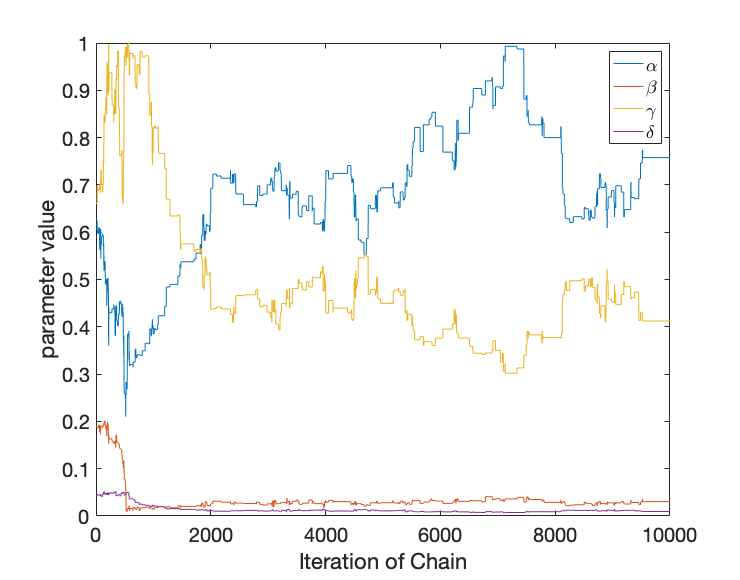
\includegraphics[width=15cm]{MCMC_figs/met_lv_final/final_mh_burninchain.png}
    \caption{Trace plot for the burn-in chain (10,000 samples) for the Metropolis MCMC parameterization of the Lotka-Volterra model. Each line shows the sampled parameter values. This figure illustrates the movement of the Markov chain as it samples parameters with the goal of finding the most likely range of values. As expected, the chain has not completely converged yet.}
    \label{fig:1mcmc}
\end{figure}
In Figure \ref{fig:1mcmc}, we can see the ``movement" of the chain as it looks around the parameter space drawing values. We have implemented and visualized a burn-in period of 10,000 chain samples. In Figure \ref{fig:1mcmc}, it appears that the values of $\alpha$ and $\gamma$ are changing fairly drastically for every sample as evidenced by their more pronounced upward and downward trends. On the other hand, $\beta$ and $\delta$ seem to have less drastic value changes appearing to reach a steady state before 2,000 samples. It is also interesting to note that the trace plots for $\alpha$ and $\gamma$ appear to mirror each other: as $\alpha$ decreases, $\gamma$ increases and vice versa. Recall from Section \ref{Lotka_Volterra_System} that $\alpha$ is the prey population increase and $\gamma$ is the natural mortality rate of the predator. In the context of this relationship, it makes sense that as prey population increases, the mortality rate of the predators decreases as their is more abundant food and as prey population decreases, the predator mortality rate increases as there is less food.
\begin{figure}[H]
    \centering
    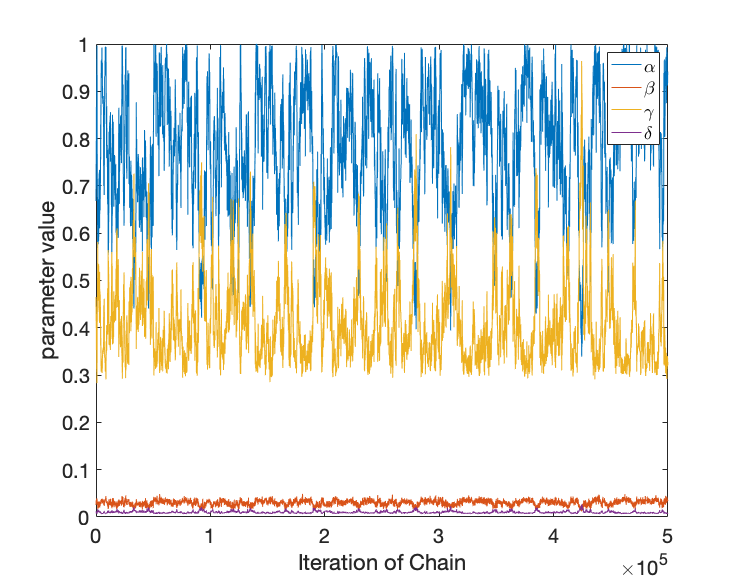
\includegraphics[width=15cm]{MCMC_figs/met_lv_final/final_mh_chain.png}
    \caption{Trace plot for the sampling chain (500,000 samples) for the DRAM MCMC parameterization of the Lotka-Volterra model. Each line shows the sampled parameter values. This figure visualizes each parameter value that has been sampled and accepted that will be used to build parameter PDFs. This chain visualization shows us that the algorithm is having a some difficult determining the most suitable mean as we see a distinct ``wave" pattern which indicates that chain mixing could be improved.}
    \label{fig:2mcmc}
\end{figure}
 In Figure \ref{fig:2mcmc}, we illustrate the final 500,000 values that our algorithm sampled. From a visual perspective, we can see that the chains appear to have achieved a steady-state; although the values still ``jump" up and down, they appear to do so around a certain value. For instance, $\alpha$ appears to move around 0.8 while $\gamma$ settles around 0.4. Often such a visual analysis of the chain as in Figure \ref{eq:2mcmc} is used to evaluate a chain's \textit{mixing time}. Briefly, mixing time refers to number of samples a chain requires to achieve a steady state and is directly related to the performance of the algorithm \cite{mixingtime}. Thus, a well-mixed chain is such a chain that in the given number of samples has achieved a steady state while a poorly mixed chain has not. Figure \ref{fig:2mcmc} demonstrates that the chain is fairly well mixed however as we will see later, it could be improved.
 \par The chain's ability to reach a steady state is important in determining the reliability of the final parameter distributions. We want our chain to reach a steady state or \emph{converge} by the time we complete sampling as this indicates the algorithm could not find ``better" or more likely values for the parameters within the constraints of the model. A \textit{burn-in} period gives the algorithm time to explore the parameter space and converge before sampling and collection for the distribution begins.
\par There are several formal techniques for confirming chain convergence, for example the Geweke diagnostic \cite{geweke1} and the Gelman-Rubin diagnostic \cite{gelman_rubin}. We use the Geweke diagnostic to quantitatively assess convergence. Next, let's look at the statistical results from our chain in Table \ref{tab:1mcmc}.
\begin{table}[H]
\centering
        \begin{tabular}{c c|c c |c c ||c}
            \hline
            \textbf{Parameter} & \textbf{Initial Value} & \textbf{Mean} & \textbf{Std} &  \textbf{Geweke} & \textbf{p-value} & \textbf{Chain Acceptance Rate}\\ 
            \cline{1-7}
            $\alpha$ & 0.625 & 0.779 & 0.134 & -0.1325 & 0.895 & \multirow{4}{*}{0.0242} \\
            $\beta$ & 0.190 & 0.0301 & 5.40e-03 & -0.1177 & 0.906\\
            $\gamma$ & 0.661 & 0.412 & 0.0871 & 0.1199 & 0.905\\
            $\delta$ & 0.0468 & 9.95e-03 & 2.30e-03 & 0.1226 & 0.902 
            \\\hline
                          \hline
        \end{tabular}
    \caption{Table listing results of the Metropolis chain. Parameter means, standard deviations, convergence diagnostics (Geweke), and the Geweke p-values are calculated. Based on the p-values values, the chain has converged for all the parameters. The chain acceptance rate is significantly less than 25\% indicating that the algorithm was likely rejecting many candidates. This makes it more likely for the algorithm to have gotten stuck in a local maximum.}
    \label{tab:1mcmc}
\end{table}
From Table \ref{tab:1mcmc}, we are most interested in the Geweke diagnostic. For now, it is enough to know that the diagnostic compares the means of the first $10\%$ and last $50\%$ of the chain. If these means are similar, it indicates that convergence occurred within the first $10\%$ of the chain's samples \cite{geweke_ppt} \cite{geweke1}. In this implementation, the Geweke value is calculated as a two-sample Z-test and a p-value is derived from the z-value. Some basic statistical knowledge is necessary to calculate and interpret the Geweke diagnostic which we explore in Appendix \ref{appendix:gewekediagnostic}. To determine convergence, we analyze the p-values. Briefly, p-values indicate evidence against a null hypothesis. In this scenario our null hypothesis is that our chain has converged (and our alternative is that the chain has not converged). The smaller the p-value, the more evidence we have to reject the null hypothesis, that is to say that it is unlikely that the chain has converged. We will use the typical p-value of 0.05 to indicate rejection of the null hypothesis. By this standard we \textit{fail} to reject our null hypothesis, thus we say that the chain has converged for all our parameters and we are confident that the parameters' mean values produce a good prediction of our model (as seen in Figure \ref{fig:5mcmc}). 
\par Finally, we can assess the performance using the chain acceptance ratio. Previous literature mathematically justifies that an acceptance rate of around $25\%$ indicates high performance of the chain \cite{convergence} \cite{converge_threshold}. However, it should be cautioned that (as with most claims of universal applications), we cannot rely solely on this diagnostic. We merely present the chain acceptance rate as one mode of investigating chain performance. An acceptance rate of 0.0242, is significantly smaller than the recommended 0.25. This indicates that our algorithm is perhaps not performing very well. With such a low acceptance rate, our algorithm seems to have rejected a majority of the candidate parameter sets. This increases the probability that the algorithm has either found a local maximum or gotten stuck in one. Due to the convergence we see using the Geweke p-values, we hypothesize that our algorithm is doing the former. A visual assessment of the mixing of the chain in Figure \ref{fig:2mcmc} seems to corroborate this idea. A well-mixed chain is defined as having explored all important regions within its stationary distribution \cite{convergence_mixing}. Visually at each sample, we want to see our chain explore the full range (given by the implementer) of the parameter value, settling around a mean value \cite{convergence_ppt}. In looking at the trace plot for $\alpha$, we see that while the chain changes values at each step, the amount by which parameter values change differs sample to sample. This results in a pronounced increase and decrease of mean (although it does still converge around a single value). In a well-mixed chain (see Figure \ref{fig:7mcmc}), we would see that parameter values differ by a very similar amount sample to sample.
Other methods for formally assessing mixing are beyond the scope of this paper \cite{convergence_mixing}.
\par The \texttt{mcmcstat} library provides functions to analyze the relationships between the parameters of our model.
\begin{figure}[H]
    \centering
    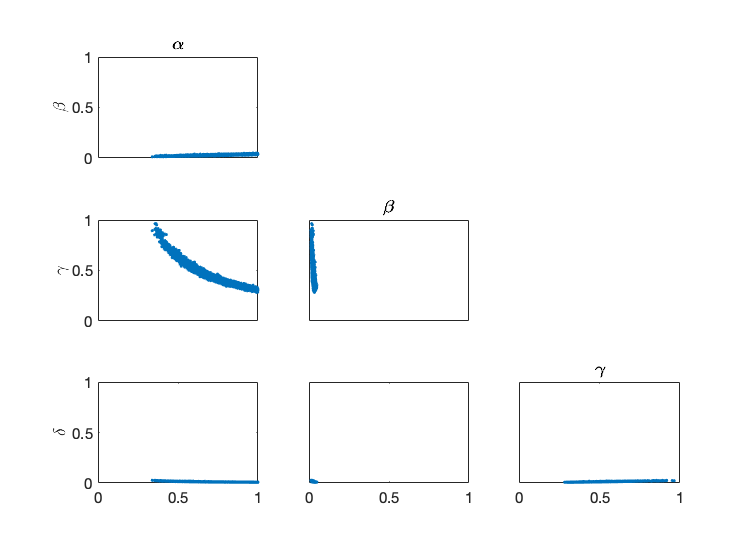
\includegraphics[width=15cm]{MCMC_figs/met_lv_final/final_mh_samples.png}
    \caption{Relationships between Lotka-Volterra parameter values per chain sample using the Metropolis MCMC algorithm. All x- and y-axes are of the same same scale respectively. Most notably there is a clear negative relationship between $\alpha$ and $\gamma$. This correlation will play a role in the algorithm's ability to choose optimal parameter values.}
    \label{fig:3mcmc}
\end{figure}
Recall that the parameter space for this model is 4-dimensional. Figure \ref{fig:3mcmc} illustrates the relationships in our parameter space as more and more values are sampled. We can see that the $\alpha \sim \gamma$ relationship is clearly negative. Recall the mirror relationship that we saw in the trace plots of these parameters in Figure \ref{fig:1mcmc}. Figure \ref{fig:3mcmc} confirms this relationship that we saw and that $\alpha$ and $\gamma$ are correlated. Ideally, we would like to see a normal clustering of values with no clear correlation. While the correlation between parameter values are a result of the model, they do impact the sampling procedure as strong correlations make it difficult to determine unique parameter sets. While we will not explore this idea of \emph{parameter identifiability} in this tutorial, we encourage the reader to consult \cite{smithCh8}. Briefly, parameter identifiability quantifies how parameter values may be correlated but can still be uniquely determined by the model \cite{smithCh8}.
\paragraph{Working with the distributions}
\par Now let's see how we can determine a posterior distribution for our parameters:
\begin{figure}[H]
    \centering
    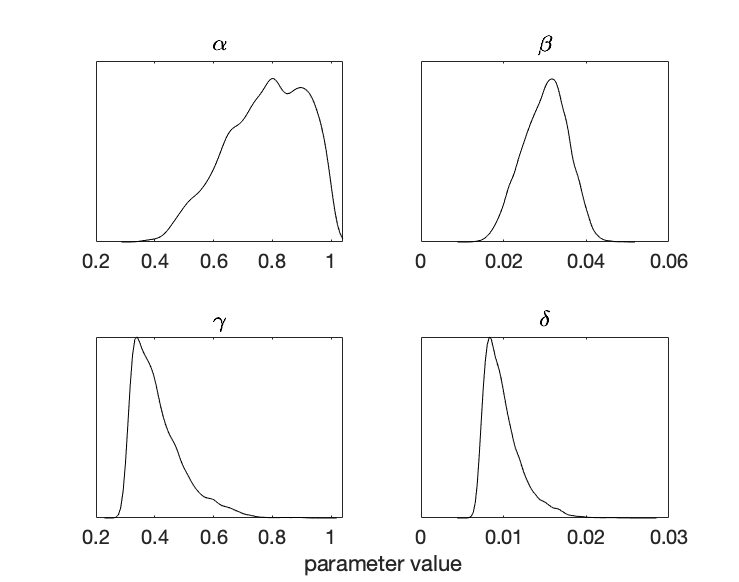
\includegraphics[width=15cm]{MCMC_figs/met_lv_final/final_mh_den.png}
    \caption{Posterior density distributions for each Lotka-Volterra model parameter using the Metropolis MCMC algorithm. The distribution for $\alpha$ is noticeably not smooth at its peak. This illustrates the algorithm's inability to find the optimal mean value for $\alpha$. Additionally, this non-smoothness is reflected in the lower Geweke value, which although indicates convergence, does not indicate such complete convergence as the other parameters.}
    \label{fig:4mcmc}
\end{figure}
By collecting the accepted values for each parameter, we can fit distributions such as those in Figure \ref{fig:4mcmc}. While we cannot definitively categorize these distributions visually, we can see that at least $\gamma$ and $\delta$ resemble some a familiar distribution, namely a lognormal distribution. It is more difficult to categorize $\alpha$ although $\beta$ appears to tend toward a normal distribution. It is useful to visualize these distributions, but they may not be directly useful. However, we can calculate their means that may be used in computations. Additionally, we make note of the relative ``bumpiness" of the peak in $\alpha$'s PDF. This indicates that the algorithm may have had difficulty in pinpointing the optimal mean value. To understand why the algorithm may have struggled to estimate $\alpha$, recall the hare population in Figure \ref{fig:0prob}. In the earlier data, the hare population has rather large spikes in population growth and the peaks around 1850 and 1870 have what appears to be 2 peaks. As the likelihood function is implemented as a sum of squares function that depends directly on the raw data, the irregularity of the data may have made it difficult for the Metropolis algorithm to pinpoint the hare population increase rate.  The lack of smoothness is also reflected in $\alpha$'s lower Geweke value; although we still conclude convergence of the chain for $\alpha$, the chain did not demonstrate the confidence of convergence as it did for the remaining 3 parameters. Next we visualize some predictions of our model using the chain samples.
\begin{figure}[H]
    \centering
    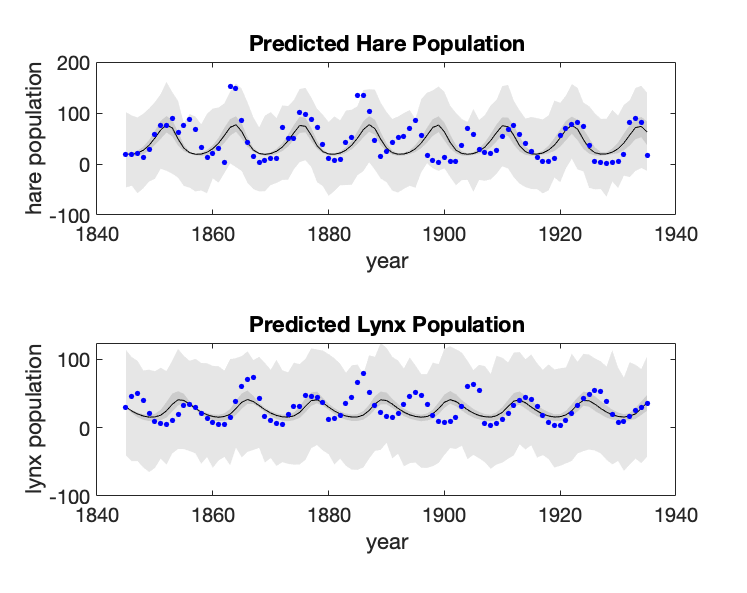
\includegraphics[width=15cm]{MCMC_figs/final_mh_modpred.png}
    \caption{Predicted hare and lynx populations using parameter values found using Metropolis MCMC. Black lines indicate the mean model prediction; gray area indicates 95$\%$ probability limits for new observations; blue points indicate original raw hare and lynx population data. For both hare and lynx populations, the Metropolis parameterization is unable to fully capture the irregular peaks in populations that occur from around 1840 to 1910. Instead, we see a symmetric periodic function for both population predictions.}
    \label{fig:5mcmc}
\end{figure}
From Figure \ref{fig:5mcmc}, we can get a visual sense of how well our sampled parameter values predict the raw data given our model. In the predicted lynx population, all of the raw data falls within our $95\%$ probability range, which tells us our predictions are doing a good job of capturing the data. In the hare population, most of the raw data falls within that $95\%$ range, although few points do not. The 95\% probability ranges help us to determine how well a majority of our sampled parameter sets capture the data. However in practice, we are most interested in the prediction that uses the mean parameter values as we are likely to only want to use a single set of parameter values in future models.
\subsection{Delayed Rejection Adaptive Metropolis} \label{Delayed_Rejection_Adaptive_Metropolis}
There are many variations of MCMC methods that can be used to parameterize biological systems, each with their own benefits. We have chosen to describe the delayed rejection adaptive Metropolis (DRAM) MCMC method to compare with the Metropolis MCMC algorithm \cite{DRAM1}. As its name suggests, DRAM builds upon several of the MCMC algorithms namely adaptive Metropolis (AM) and delayed rejection (DR) and is often used in order to allow for better adaptation of the sampling chain as time goes on \cite{DRAM1}. Like most MCMC methods, DRAM requires initialization of proposal, likelihood, and prior distributions. However, while the proposal distribution of Metropolis MCMC is assumed (via a covariance matrix) given some \emph{a priori} information about parameter values and variability, in adaptive methods such as DRAM, posterior information learned during the progression of the algorithm is immediately incorporated and the algorithm adjusted. In order to understand the DRAM algorithm, it is useful to begin with its two parts.
\subsubsection{Adaptive Metropolis}
The adaptive Metropolis method is an optimization of of simpler MCMC algorithms as it allows the algorithm to move quickly through parameter space of low probability \cite{collis}, \cite{adaptive_andrieu}. The adaptive algorithm does this by updating its proposal distribution as sampling occurs thus creating a more informed pool from which candidates are drawn. The adaptive Metropolis algorithm proceeds as follows:
\begin{tcolorbox} \label{box:am}
\textbf{\underline{Adaptive Metropolis Algorithm (with an uninformative prior)}}
\begin{enumerate}
\item Set number samples to take, $N$; number of candidates to sample before updating the proposal distribution, $k_0$; and burn-in period, $k_b$
    \item Determine an initial parameter guess $\theta^0 = argmin_q \sum_{i=1}^{n}[M_i - f_i(\theta)]^2]$
    \item Set $SS_{\theta^0} = \sum_{i = 1}^{n}[y_i - f_i(\theta^0)]^2$ (for likelihood)
    \item Compute an initial variance estimate $s_0^2 = \frac{SS_{\theta^0}}{n-p}$ ($n =$ number of data points, $p = $ number of parameters)
    \item Construct an initial proposal covariance matrix $V_0$ 
    \item For each iteration of the chain, $k = 1,...,N$
    \begin{enumerate}
        \item Sample $z \sim N(0,I_p)$
        \item Construct candidate $\theta^* = \theta^{k-1}+ V_0z$
        \item Compute $SS_{\theta^*} = \sum_{i = 1}^{n}[y_i - f_i(\theta^*)]^2$ (likelihood sum of squares)
        \item Compute acceptance criterion
            \begin{center}
                $\alpha(\theta^* | \theta^{k-1}) = min(1, e^{-[SS_{\theta^*}-SS_{\theta^{k-1}}/2s_{k-1}^2]})$
            \end{center}
        \item Accept $\theta^*$ with a probability 1 if $\alpha \geq 1$ and accept it with probability $\alpha$ if $\alpha < 1$.
        \begin{itemize}
            \item If $\theta^*$ is accepted
            \begin{center}
                $\theta^k = \theta^*$, $SS_{\theta^k} = SS_{\theta^*}$
            \end{center}
            \item Else
            \begin{center}
                $\theta^k = \theta^{k-1}$, $SS_{\theta^k} = SS_{\theta^{k-1}}$
            \end{center}
        \end{itemize}
        \item If $k > k_b$ collect $\theta^*$ in posterior matrix $P$, else discard
        \item Update $s_k^2 = \frac{SS_{\theta^k}}{n-p}$
    \end{enumerate}
    \begin{tcolorbox}[colback=red!5,colframe=red!75!black,title=Adaptive Step]
    \item If $k = k_0$ adaptation commences: the initial $V_0$ is updated to the covariance matrix, $V_{k}$ \label{step:7adapt}
    \begin{center}
       $V_{k} = s_{p}cov(\theta^{0},\theta^{1},...,\theta^{k-1}) + \epsilon I_{p}$
    \end{center}
    \end{tcolorbox}
    
\end{enumerate}
\emph{Based on Smith (2014) Algorithm 8.8}
\end{tcolorbox}
\par We want to choose $k_0$ to balance a mixing with sufficient diversity of points to ensure a non-singular covariance matrix ($V$). Note that $V$ must be non-singular (i.e. invertible) because the calculating the proposal distribution requires computing $V$'s inverse \cite{WallinBolin2018nonsingcov}. Shorter adaptation intervals tend to produce better mixing and higher acceptance ratios \cite{convergence_mixing} and thus, the chain is more responsive to new data from parameter space not previously explored. In practice, $k_0$ is often 100 \cite{smithCh8}. 
\par The fundamental steps of the AM algorithm are taken directly from the Metropolis algorithm, in both algorithms sample, accept, and reject candidate parameter sets in the same way. Recall from the Metropolis algorithm that in Step 6a $z$ is the random component of selecting a parameter set and is what makes each $\theta^*$ unique even if multiple $\theta^*$s are found using the same $\theta^{k-1}$. Step \ref{step:7adapt} of this algorithm is the adaptive step of the AM algorithm. This step updates the current covariance matrix $V_0$ according to the covariances between the accepted parameter sets. Here, $s_{p}$ is a design parameter that depends on the dimension ($p$) of the parameter space; a common choice is $s_{p} = 2.38^{2}/p$ \cite{smithCh8}. The term $\epsilon I_{p}$ refers to an identity matrix of dimension $p$-by-$p$ (to ensure $V_{k}$ is positive definite). Often, $\epsilon = 0$ \cite{smithCh8}.
\par While Steps 1-6 are directly adapted from the Metropolis MCMC algorithm, Step 7 in the above algorithm is the new adaptive step that allows the algorithm to traverse parameter space of lower probability efficiently.

\subsubsection{Delayed Rejection}
\par The delayed rejection MCMC improves the efficiency of other MCMC methods by increasing the transition probability of parameters leading to improvement in chain mixing \cite{trias2009delayed}. In the standard Metropolis algorithm, when a candidate parameter set $\theta^*$ is rejected (with its prescribed acceptance ratio $\alpha$), the current step parameter set, $\theta^{k-1}$, is retained and $\theta^*$ is discarded before choosing the next sample. In the \emph{delayed rejection} (DR) algorithm, when $\theta^*$ is rejected, alternative candidates $\theta^{*j}$ are constructed and considered instead of immediately reverting back to $\theta^{k-1}$. We can specify the number of alternatives our algorithm will propose before moving on to the next iteration of the chain. By sampling multiple candidates under the same sampling conditions (recall Step \ref{step:6met}g of the Metropolis algorithm) we allow the algorithm to consider parameter space with lower probability that, in the Metropolis algorithm, may have been omitted. Additionally, these alternative candidates prevent the algorithm from getting stuck in local maxima or minima. Loosely this works as follows: when we accept a candidate parameter, its values become the basis of constructing the next proposed candidate (recall \textbf{Steps \ref{step:6met}a} and \textbf{\ref{step:6met}b} of the Metropolis algorithm). Therefore, the next time we reject a candidate, the subsequent candidate must be constructed using only the same information as the most recently accepted parameter set. This is computationally inefficient as we have already searched this particular parameter space, yet we are forced to draw again from the same space and in effect, we have not explored anything new. When this immediate rejection process is compounded, we may encounter long periods in which we propose many candidates only using a single set of parameter values, thus we are not exploring the whole parameter space and run the risk of staying in local maxima.
\par In order to work with alternative candidates, we must redefine the acceptance criterion, $\alpha$. We follow an explanation from \cite{smithCh8}.\\
For example, $\theta^{*2}$, a second-stage candidate, is chosen using proposal function
\begin{equation} \label{eq:17mcmc}
J_{*2}(\theta^{*2}|\theta^{k-1},\theta^*) \sim N(\theta^{k-1}, \gamma^2V)
\end{equation} 
where $V$ is the covariance matrix informing the proposal distribution. $J_{*2}(\theta^{*2}|\theta^{k-1},\theta^*)$ indicates that we propose $\theta^{*2}$ having started at $\theta^{k-1}$ and rejected $\theta^*$. Finally, $\gamma < 1$ tunes the second-stage proposal function and increases mixing \cite{smithCh8}. The acceptance criteria for the second-stage candidate thus is\\
\begin{equation} \label{eq:18mcmc}
\alpha_{*2}(\theta^{*2}|\theta^{k-1}, \theta^*) = min(1, \frac{P(\theta^{*2}|M)J(\theta^*|
    \theta^{*2})[1-\alpha(\theta^*|\theta^{*2})]}{P(\theta^{k-1}|M)J(\theta^*|\theta^{k-1})[1-\alpha(\theta^*|\theta^{k-1})]})
\end{equation}
With these additional steps, we outline the DR algorithm.
\begin{tcolorbox} \label{alg:DRmcmc}
\textbf{\underline{Delayed Rejection Algorithm (with an uninformative prior)}}
\begin{enumerate}

\item Set number samples to take, $N$; choose number of alternatives, $n_{alt}$; and determine a burn-in period, $k_b$
    \item Determine an initial parameter guess $\theta^0 = argmin_q \sum_{i=1}^{n}[M_i - f_i(\theta)]^2]$
    \item Set $SS_{\theta^0} = \sum_{i = 1}^{n}[y_i - f_i(\theta^0)]^2$ (for likelihood)
    \item Compute an initial variance estimate $s_0^2 = \frac{SS_{\theta^0}}{n-p}$ ($n =$ number of data points, $p = $ number of parameters)
    \item Construct a proposal covariance matrix $V$ 
    \item For each iteration of the chain, $k = 1,...,N$
    \begin{enumerate}
        \item Sample $z \sim N(0,I_p)$ 
        \item Construct candidate $\theta^* = \theta^{k-1}+ V_0z$
        
        \item Compute $SS_{\theta^*} = \sum_{i = 1}^{n}[y_i - f_i(\theta^*)]^2$ (likelihood sum of squares)
        \item Compute acceptance criterion
            \begin{center}
                $\alpha(\theta^* | \theta^{k-1}) = min(1, e^{-[SS_{\theta^*}-SS_{\theta^{k-1}}/2s_{k-1}^2]})$
            \end{center}
        \item Accept $\theta^*$ with a probability 1 if $\alpha \geq 1$ and accept it with probability $\alpha$ if $\alpha < 1$.
        \begin{enumerate}
            \item If $\theta^*$ is accepted, proceed to next sample
            \begin{center}
                $\theta^k = \theta^*$, $SS_{\theta^k} = SS_{\theta^*}$
            \end{center}
            \begin{tcolorbox}[colback=red!5,colframe=red!75!black,title=Delayed Rejection]
        
            \item Else enter \textbf{delayed rejection process} while $n_i \leq n_{alt}$
            \begin{enumerate}
                \item Set design parameter $\gamma < 1$
                \item Sample $z_{n_i} \sim N(0,I_p)$ 
                \item Construct i-stage alternative $\theta^{*i} = \theta^{k-1} + \gamma Vz_{n_i}$
                \item Compute acceptance criterion
                \begin{center}
                  $\alpha_{*i}(\theta^{*i}|\theta^{k-1}, \theta^*) = min(1, \frac{P(\theta^{*i}|M)J(\theta^*|
    \theta^{*i})[1-\alpha(\theta^*|\theta^{*2})]}{P(\theta^{k-1}|M)J(\theta^*|\theta^{k-1})[1-\alpha(\theta^*|\theta^{k-1})]})$
                \end{center}
                \item Accept $\theta^{*i}$ with a probability 1 if $\alpha_{*i} \geq 1$ and accept with probability $\alpha_{*i}$ if $\alpha_{*i} < 1$.
            \end{enumerate}
            \end{tcolorbox}
        \end{enumerate}
        \item If $k > k_b$ collect $\theta^*$ in posterior matrix $P$, else discard
        \item Update $s_k^2 = \frac{SS_{\theta^k}}{n-p}$
    \end{enumerate}
\end{enumerate}
\emph{Based on Smith (2014) Algorithm 8.8}
\end{tcolorbox}
In Step 1, we can choose to determine a specific number of alternative parameter sets that the algorithm will propose, $n_alt$, before rejecting and proceeding to the next iteration of the algorithm. Note that if the algorithm is allowed to propose infinite alternatives, the efficiency of the algorithm is likely to increase (possible to infeasible levels). In Step 6e.ii we see the delayed rejection process. This process is very similar to the Metropolis method of accepting and rejecting candidate parameter sets. In Step 6e.ii.B we see that again we have $z_{n_i} \sim N(0, I_p$ which is the random component of selecting a parameter set and is what makes each $\theta^*i$ unique as each alternative candidate is sampled using the same $\theta^{k-1}$.
\par Now we have an understanding of both the delayed rejection and adaptive Metropolis MCMC algorithms, we can construct the final DRAM algorithm. We will do this in the following section by using Steps 1-6 of the Metropolis algorithm as a foundation and incorporating Step 7 of the adaptive Metropolis algorithm and Step 6e(ii) of the delayed rejection algorithm.
\subsubsection{Constructing the DRAM Algorithm}
Now that we have the basis for the two components of the delayed rejection adaptive Metropolis algorithm, all that is left to do is merge them. Using the foundation of the Metropolis algorithm, we add an adaptive step and a delayed rejection process. In the DRAM algorithm, the adaptive Metropolis and delayed rejection work together: AM updates the proposal via previously accepted candidates and the covariance matrix and DR alters the proposal function to improve mixing.
\begin{tcolorbox}
\textbf{\underline{The DRAM Algorithm (with an uninformative prior)}} 
\begin{enumerate}
\item Set number of samples to take, $N$, adaptive chain length, $k_0$, number of alternatives, $n_{alt}$, and burn-in period, $k_b$
    \item Determine an initial parameter guess $\theta^0 = argmin_q \sum_{i=1}^{n}[M_i - f_i(\theta)]^2]$
    \item Set $SS_{\theta^0} = \sum_{i = 1}^{n}[y_i - f_i(\theta^0)]^2$ (for likelihood)
    \item Compute an initial variance estimate $s_0^2 = \frac{SS_{\theta^0}}{n-p}$ ($n =$ number of data points, $p = $ number of parameters)
    \item Construct an initial covariance matrix $V_0$ 
    \item For each iteration of the chain, $k = 1,...,N$
    \begin{enumerate}
        \item Sample $z \sim N(0,I_p)$
        \item Construct candidate $\theta^* = \theta^{k-1}+ V_0z$
        \item Compute $SS_{\theta^*} = \sum_{i = 1}^{n}[y_i - f_i(\theta^*)]^2$ (likelihood sum of squares)
        \item Compute acceptance criterion
            \begin{center}
                $\alpha(\theta^* | \theta^{k-1}) = min(1, e^{-[SS_{\theta^*}-SS_{\theta^{k-1}}/2s_{k-1}^2]})$
            \end{center}
        \item Accept $\theta^*$ with a probability 1 if $\alpha \geq 1$ and accept it with probability $\alpha$ if $\alpha < 1$.
        \begin{tcolorbox}[colback=red!5,colframe=red!75!black,title=DRAM Step]
        \begin{enumerate}
            \item If $\theta^*$ is accepted, proceed to next sample
            \begin{center}
                $\theta^k = \theta^*$, $SS_{\theta^k} = SS_{\theta^*}$
            \end{center}
            \item Else enter \textbf{delayed rejection process} while $n_i \leq n_{alt}$
            \begin{enumerate}
                \item Set design parameter $\gamma < 1$
                \item Sample $z_{n_i} \sim N(0,I_p)$ 
                \item Construct i-stage alternative $\theta^{*i} = \theta^{k-1} + \gamma Vz_{n_i}$
                \item Compute acceptance criterion
                \begin{center}
                  $\alpha_{*i}(\theta^{*i}|\theta^{k-1}, \theta^*) = min(1, \frac{P(\theta^{*i}|M)J(\theta^*|
    \theta^{*i})[1-\alpha(\theta^*|\theta^{*2})]}{P(\theta^{k-1}|M)J(\theta^*|\theta^{k-1})[1-\alpha(\theta^*|\theta^{k-1})]})$
                \end{center}
                \item Accept $\theta^{*i}$ with a probability 1 if $\alpha_{*i} \geq 1$ and accept with probability $\alpha_{*i}$ if $\alpha_{*i} < 1$.
            \end{enumerate}
            
        \end{enumerate}
        \item If $k = k_0$ adaptation commences: the initial $V_0$ is updated to the covariance matrix, $V_{k}$
       
        \begin{center}
            $V_{k} = s_{p}cov(\theta^{0},\theta^{1},...,\theta^{k-1}) + \epsilon I_{p}$
        \end{center}
        \end{tcolorbox}
        \item If $k > k_b$ collect $\theta^*$ in posterior matrix $P$, else discard
        \item Update $s_k^2 = \frac{SS_{\theta^k}}{n-p}$
        
    \end{enumerate}
    
\end{enumerate}
\emph{Based on Smith (2014) Algorithms 8.8 and 8.10}
\end{tcolorbox}
We have now combined the adaptive Metropolis and delayed rejection processes outlined in Steps 6e and 6f. In the next section we will estimate parameters for the Lotka-Volterra system and compare results with the Metropolis MCMC parameterization.

\subsubsection{Parameterizing Lotka-Volterra}
As with the Metropolis MCMC, DRAM was used to estimate parameters of the Lotka-Volterra system. We implemented likelihood, and proposal distributions identical to those used in the Metropolis parameterization (Steps 3 and 5). We implemented a log-uniform prior function, however we used a different range for each parameter value (see Table \ref{table:ParameterNotationAppendix} in Appendix \ref{general_appendix}). The number of iterations was also held constant, the adaptive interval $k_0$ was defined to be 100, a common default in DRAM, and 2 alternate candidates were specified (this number is a default setting of the MATLAB \texttt{mcmcstat} library function \texttt{mcmcrun}; Step 1). Just as in the Metropolis parameterization, we first visualize the burn-in and sampled chains.
\begin{figure}[H]
    \centering
    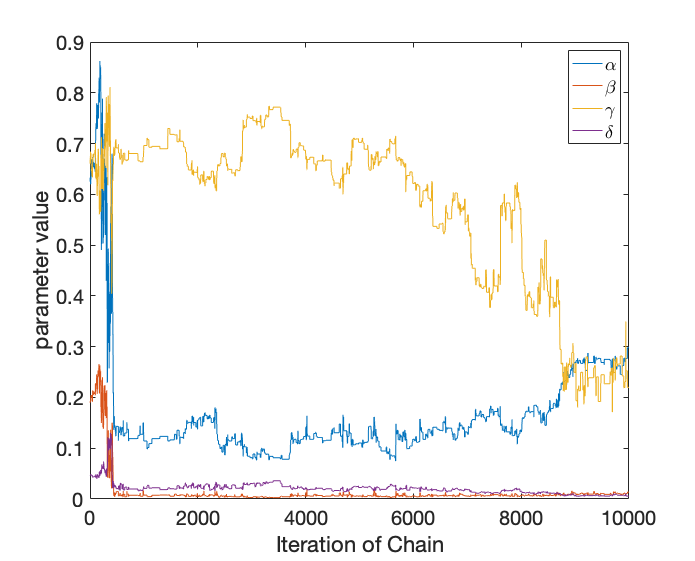
\includegraphics[width=15cm]{MCMC_figs/met_lv_final/final_dram_burninchain.png}
    \caption{Burn-in chain (10,000 samples) for the DRAM MCMC parameterization of the Lotka-Volterra model. Each line shows the sampled parameter values. This figure illustrates the movement of the Markov chain as it samples parameters with the goal of finding the most likely range of values. As expected, the chain has not converged for all the parameters yet.}
    \label{fig:6mcmc} 
\end{figure}
\begin{figure}[H]
    \centering
    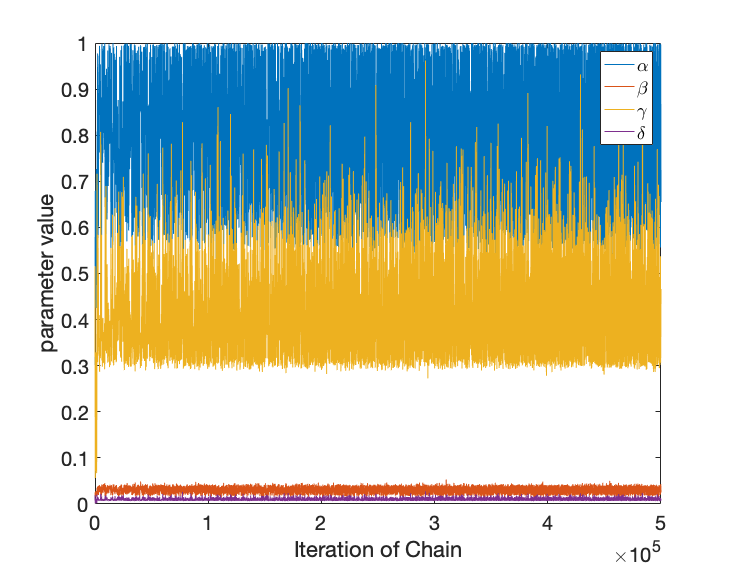
\includegraphics[width=15cm]{MCMC_figs/met_lv_final/final_dram_chain.png}
    \caption{Sampling chain (500,000 samples) for the DRAM MCMC parameterization of the Lotka-Volterra model. Each line shows the sampled parameter values. This figure visualizes each parameter value that has been sampled and accepted that will be used to build parameter PDFs. This chain visualization shows a ``fuzzy caterpillar" sampling pattern indicative of a well-mixed chain.}
    \label{fig:7mcmc}
\end{figure}
Figure \ref{eq:6mcmc} shows the chain's exploration of the parameter space during the burn-in period (10,000 samples). From a preliminary visual analysis of this chain, we can see that $\alpha$, $\beta$, and $\delta$ seem to find their steady states fairly quickly ($<$ 2,000 samples). Additionally, $\gamma$ seems to trend toward its optimal value range more immediately than in the Metropolis algorithm (Figure \ref{fig:1mcmc}). From 0 to around 9,000 samples, $\gamma$ generally trends downward until it hits a value range of $0.3$ to $0.2$. In Figure \ref{fig:7mcmc}, we illustrate the final 500,000 values that our algorithm sampled. From a visual perspective, this chain appears to demonstrate good mixing as the chain appears to have settled in a steady state for each parameter. This is evidenced by the lack of a ``wave" pattern that we saw in Figure \ref{fig:2mcmc} and thus, a lack of increasing or decreasing trends of parameter values. For instance, $\alpha$ appears to move around 0.8 while $\gamma$ settles around 0.4. Statisticians have often referred to a well-mixed plot as resembling a ``fuzzy caterpillar", due to its dense and somewhat spiked appearance \cite{fuzzy_caterpillar}. However, the means of these well-mixed plots are relatively constant mean and suggest that the values of the chain are no longer changing and are therefore in a steady state.
\par Next, let's look at the statistical results from our chain in Table \ref{tab:2mcmc}.
%           
\begin{table}[H]
\centering
        \begin{tabular}{c c |c c | c c ||c}
            \hline
            \textbf{Parameter} & \textbf{Inital Value} & \textbf{Mean} &  \textbf{Std} & \textbf{Geweke} & \textbf{p-value} & \textbf{Chain Acceptance Rate}\\ 
            \cline{1-7}
            $\alpha$ & 0.625 & 0.787 & 0.139 & 0.0219 & 0.983 & \multirow{4}{*}{0.241} \\
            $\beta$ & 0.190 & 0.0303 & 5.58e-03 & 0.0136 & 0.989\\
            $\gamma$ & 0.661 & 0.407 & 0.0908 & -0.0867 & 0.931\\
            $\delta$ & 0.0468 & 9.83e-03 & 2.39e-03 & -0.0838 & 0.933
             \\\hline
                          \hline
                           
        \end{tabular}
    \caption{Table listing results of the DRAM chain. Parameter means, standard deviations, the convergence diagnostic (Geweke), and the Geweke p-values are calculated. Based on the Geweke p-values values, we conclude that the chain has converged for all the parameters. The chain acceptance rate is very close to the 25\% threshold indicating that the algorithm was able to effectively search the parameter space.}
    \label{tab:2mcmc}
\end{table}
We can use the parameter means and standard deviations to find the optimal range of parameter values for this model. We look to the Geweke p-values to quantitatively determine convergence. We see that all of our p-values are greater than 0.05 and thus we fail to reject the null hypothesis that the chain has converged.
Thus we say that the chain has converged for all our parameters and we are confident that the parameters' mean values produce a good prediction of our model (as seen in Figure \ref{fig:10mcmc}). Lastly, we look at the chain's acceptance ratio 
\par We look again to the chain's acceptance rate and the visual assessment of mixing to help us analyze the chain's performance. In Table \ref{tab:2mcmc}, we see that the acceptance rate is very close to the proposed indication of good performance, $25\%$ acceptance. This leads us to believe that our chain was able to effectively search the parameter space. Intuitively, we expect the DRAM method to have a higher acceptance rate than the Metropolis method because we are able to propose several alternative candidates instead of immediately rejecting a sample. This increases the probability of accepting at any iteration of the algorithm. We further validate this belief by looking at the trace plots of the chains in Figure \ref{fig:7mcmc}. Figure \ref{fig:7mcmc} shows us that our chain is well-mixed for each of our parameters as it appears our chain has reached a steady-state for each parameter value. 
\par Let's look at the relationships between parameters as the chain samples.
\begin{figure}[H]
    \centering
    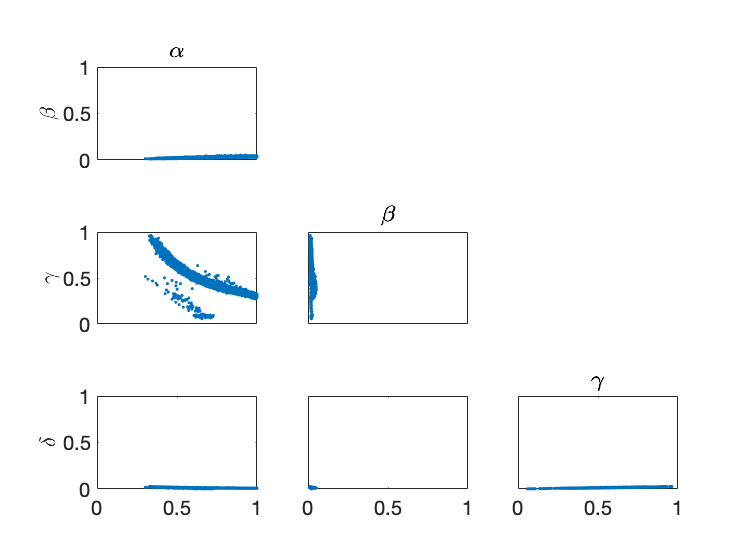
\includegraphics[width=15cm]{MCMC_figs/met_lv_final/final_dram_samples.png}
    \caption{Correlations between Lotka-Volterra parameter values per chain sample using the DRAM MCMC algorithm. There is a clear negative correlation between $\alpha$ and $\gamma$. Recalling the idea of \textit{parameter identifiability}, this may have an impact on algorithm's sampling ability.}
    \label{fig:8mcmc}
\end{figure}
Similarly to the correlation that we saw in Figure \ref{fig:3mcmc}, $\alpha$ and $\gamma$ have a strong negative relationship. However, we see what appears to be two clusters within the $\alpha \sim \gamma$ plot. This indicates that perhaps the algorithm had discovered two local maxima. However, we saw that the $\alpha$'s Geweke diagnostic from the DRAM parameter estimation was greater than the Metropolis diagnostic, indicating a higher confidence in convergence. Due to the sampling methodology of the DRAM algorithm, we hypothesize that the cluster with more samples is the global maximum and the other cluster may be a local maximum.
\paragraph{Working with the distributions}
We visualize the posterior PDFs for the system's parameters:
\begin{figure}[H]
    \centering
    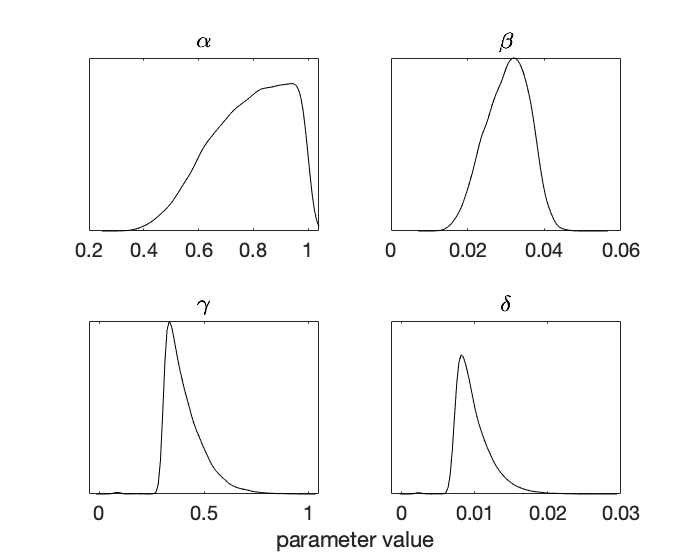
\includegraphics[width=15cm]{MCMC_figs/met_lv_final/final_dram_den.png}
    \caption{Posterior density distribution for each Lotka-Volterra parameter using the DRAM MCMC algorithm. Unlike the PDFs produced by the Metropolis MCMC algorithm, these PDFs appear fairly smooth. This indicates that the algorithm was more successful at finding global maxima.}
    \label{fig:9mcmc}
\end{figure}
We will perform a more thorough comparison of the two MCMC algorithms, but for now, we can see that like the Metropolis MCMC algorithm, we produce posterior density functions for each parameter in our model. We note that the $\alpha$ distribution appears smoother than its distribution produced by the Metropolis algorithm, this corroborates our earlier analyses of clear convergence and the location of a global maximum. Similarly to the Metropolis PDFs, we cannot strictly classify these distributions as normal. Instead, we can see how these sampled parameter sets perform against our original data.
\begin{figure}[H]
    \centering
    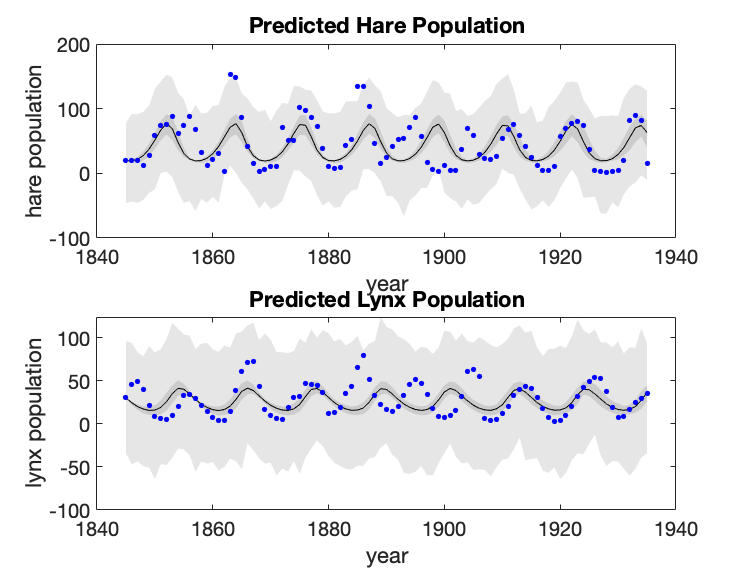
\includegraphics[width=15cm]{MCMC_figs/final_dram_modpred.png}
    \caption{Predicted hare and lynx populations using parameter values found using DRAM MCMC. Black lines indicate the mean model prediction; gray area indicates 95$\%$ probability limits for new observations; blue points indicate original raw hare and lynx population data. We can see that the prediction is having difficulty capturing the beginning of the original data (1840 to $\sim$ 1900). However, the prediction appears to capture the end behavior fairly well for both hare and lynx populations.}
    \label{fig:10mcmc}
\end{figure}
Figure \ref{fig:10mcmc} shows us a $95\%$ probability limit for model predictions using the parameter sets sampled during DRAM. Ideally, we would like to see a smaller range in these prediction. The line in black indicates the model's prediction given the ``best" set of parameters. While our probability range appears wide, particularly for the lynx population, we note that the best predicted model (black line) fits the original data pretty well, especially toward the end of the time span.
\subsection{Comparing Metropolis and DRAM MCMC Methods} \label{Comparing Metropolis_and_DRAM_MCMC_Methods}
Now we have seen two MCMC methods that we can use to parameterize a biological ODE model. Before moving on to parameterize the Type 1 Diabetes model, it is useful to compare results of these two methods to see if one does a ``better" job of parameter estimation. Recall that Metropolis MCMC is likely to find a local maximum of parameter values. But true parameter distributions may be bi- or multi-modal, that is between maxima, there are areas of low probability. Due to its method of sampling, the Metropolis algorithm is less likely to search areas of low probability. However, DRAM's sampling method allows it to traverse these areas of lower probability. Figure \ref{fig:globalmax} illustrates DRAM's ability to find multiple local maxima and eventually a global maximum.
\begin{figure}[H]
    \centering
    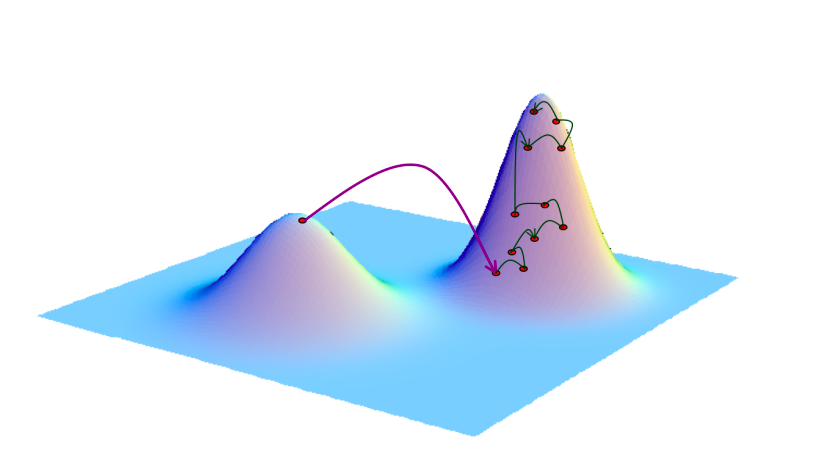
\includegraphics[width=15cm]{MCMC_figs/dram_t1d_final/multimodal_search.png}
    \caption{Graphical representation of how the DRAM can efficiently explore different maxima of the target distribution. Areas in purple tones indicate ares of higher probability parameter space, while areas in blue indicate areas of lower probability. This figure is adapted from Figure 3 of the reference \cite{trias2009delayed}.}
    \label{fig:globalmax}
\end{figure}
\par To compare the performace of the Metropolis and the DRAM MCMC methods on estimating the Lotka-Volterra model parameters, we first compare the sampling chains
\begin{figure}[H]
\begin{subfigure}{.5\textwidth}
  \centering
  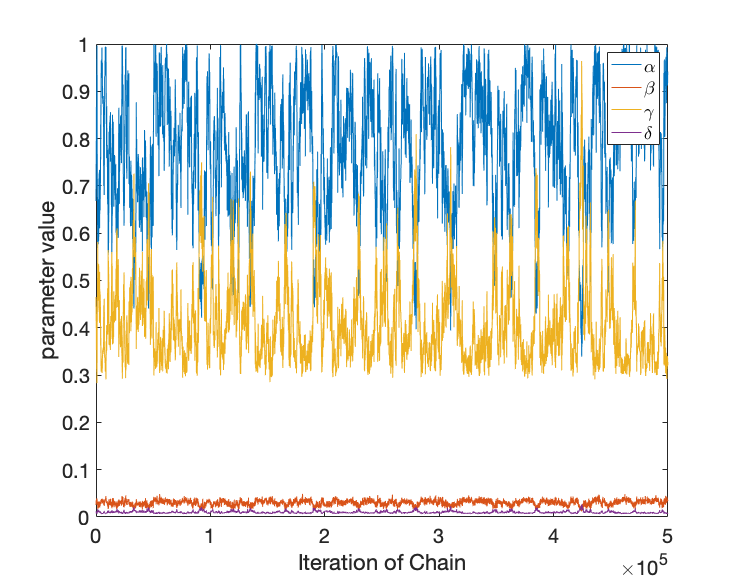
\includegraphics[width=1\linewidth]{MCMC_figs/met_lv_final/final_mh_chain.png}
  \caption{Metropolis MCMC sample chain.}
  \label{fig:11amcmcm}
\end{subfigure}
\begin{subfigure}{.5\textwidth}
  \centering
  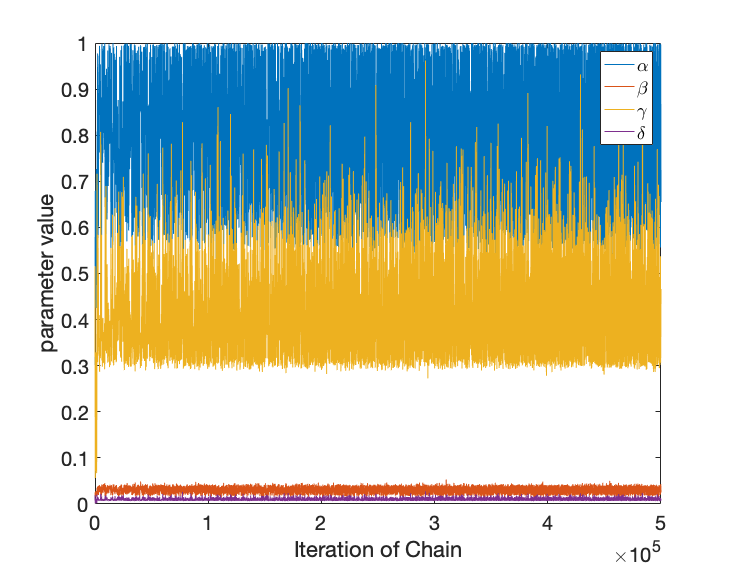
\includegraphics[width=1\linewidth]{MCMC_figs/met_lv_final/final_dram_chain.png}
  \caption{DRAM MCMC sample chain}
  \label{fig:11bmcmcm} 
\end{subfigure}
\caption{Comparing visual results of the sample chains from Metropolis and DRAM MCMC. The DRAM chain exhibits better mixing as it has the distinct ``fuzzy caterpillar" pattern.}
\label{fig:11mcmc}
\end{figure}
As we mentioned earlier, the ideal chain would be ``fuzzy catepillar-like" and we see this illustrated well in the DRAM algorithm, Figure \ref{fig:11bmcmcm}. It seems that the Metropolis chain has not done as good a job of sampling the parameter space, Figure \ref{fig:11amcmcm}. This so far this suggests that the DRAM is doing a better job of exploring the sampling space.
\par Next let's compare the computed results of these chains
%dram: .2406
% 0.0242
\begin{table}[H]
\centering
        \begin{tabular}{c | c | c c | c || c}
            \cline{1-6}
           \textbf{Parameter} & \textbf{Algorithm} &  \textbf{Mean} & \textbf{Std} &  \textbf{Geweke p-values} & \textbf{Chain Acceptance Rate}\\ 
            \cline{1-6}
            
            \multirow{2}{*}{\textbf{$\alpha$}} & Met & 0.779 & 0.134 & 0.895 & \multirow{4}{*}{\textbf{Met: 0.0242}}\\
            & DRAM & 0.787 & 0.139 & 0.983 & \\\cline{1-5}
            \multirow{2}{*}{\textbf{$\beta$}} & Met & 0.0301 & 5.40e-03 & 0.906 \\
            & DRAM & 0.030 & 5.58e-03 & 0.989 & \\ \cline{1-5}
            \multirow{2}{*}{\textbf{$\gamma$}} & Met & 0.412 & 0.0871 & 0.905 & \multirow{4}{*}{\textbf{DRAM: 0.2406}}\\
            & DRAM & 0.407 & 0.0908 & 0.931\\ \cline{1-5}
            \multirow{2}{*}{\textbf{$\delta$}} & Met & 9.95e-03 & 2.30e-03 & 0.902\\
            & DRAM & 9.83e-03 & 2.39e-03 & 0.933
             \\\hline
             \hline
        \end{tabular}
    \caption{Comparison of the results of the Metropolis and DRAM MCMC chains per parameter. There do not appear to be any significant differences in parameter values between the two algorithms. The only significant difference between the Geweke p-values occurs for $\alpha$. The DRAM appears to reach a better convergence than the Metropolis algorithm. The DRAM chain acceptance rate is significantly closer to the indicative threshold of 25\%. We do not yet discern any significant differences between the performances of each chain.}
    \label{tab:3mcmc}
\end{table}


We do not see any significant differences in individual parameter values between the two algorithms. While both p-values for $\alpha$ indicate that we fail to reject that the chain has converged, we note the difference as a possible explanation for the visual difference between $\alpha$'s PDFS. In Figure \ref{fig:4mcmc} we saw a lack of smoothness, while in Figure \ref{fig:9mcmc} we did see a more smooth distribution. Lastly we note the difference in chain acceptance rates. While not a perfect indicator of chain performance, we note that the DRAM algorithm's chain acceptance rate is much closer to the general threshold of 25\% acceptance. 

\par Next, we visually compare the PDFs of each parameter from both MCMC algorithms.
\begin{figure}[H]
    \centering
    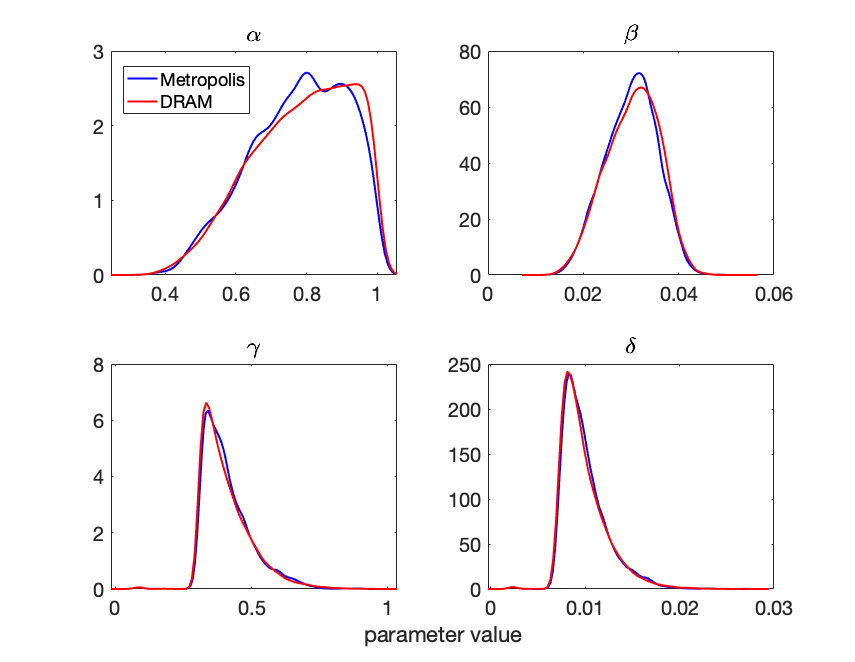
\includegraphics[width=15cm]{MCMC_figs/met_lv_final/overlaid_param_pdfs.png}
    \caption{Parameter posterior density distributions from both the Metropolis and DRAM parameterizations plotted together. We can see that the distributions are generally very similar as was evidenced in Table \ref{tab:3mcmc}. Visually, the distributions for $\alpha$ and $\gamma$ appear to differ the most.}
    \label{fig:overlayPDF_met}
\end{figure}
We can see that between the two algorithms, all of the parameters have very similar distribution shapes. In particular, the PDFS of $\gamma$ and $\delta$ are very similar. On the other hand, $\alpha$ and $\beta$ appear to differ more. Most notably, the Metropolis PDF for $\alpha$ is less smooth than that of the DRAM and appears to have 2 smaller peaks. Earlier, we discussed this visual discrepancy in terms of the statistical analysis of convergence with the Geweke p-values. Indeed, here we can see that as the $\alpha$ p-value from the Metropolis was the smallest, the corresponding PDF is the least smooth. Despite these few discrepancies, we believe that both the Metropolis and DRAM algorithms are producing comparable distributions for all the parameters.
\par Below we do a second visual assessment of the difference between means of parameters between distributions.
\begin{figure}[H]
\begin{subfigure}{.5\textwidth}
  \centering
  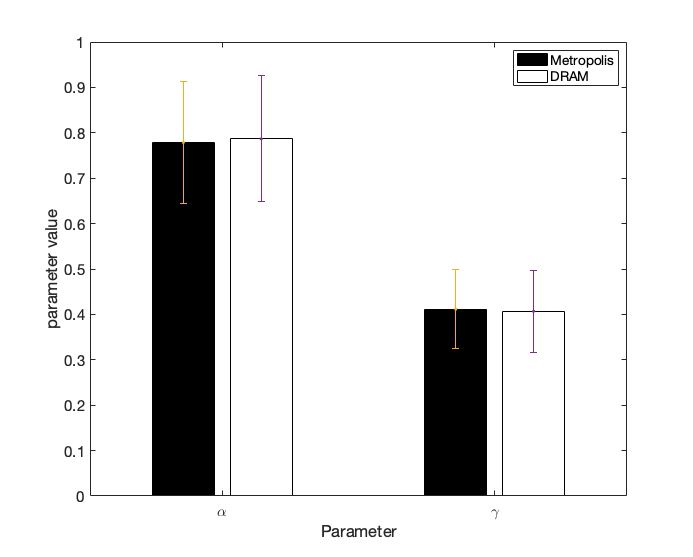
\includegraphics[width=1\linewidth]{MCMC_figs/met_lv_final/mh_dram_paramComp1.png}
  \caption{Comparison of means for $\alpha$ (left) and $\gamma$ (right).}
  \label{fig:12amcmcm}
\end{subfigure}
\begin{subfigure}{.5\textwidth}
  \centering
  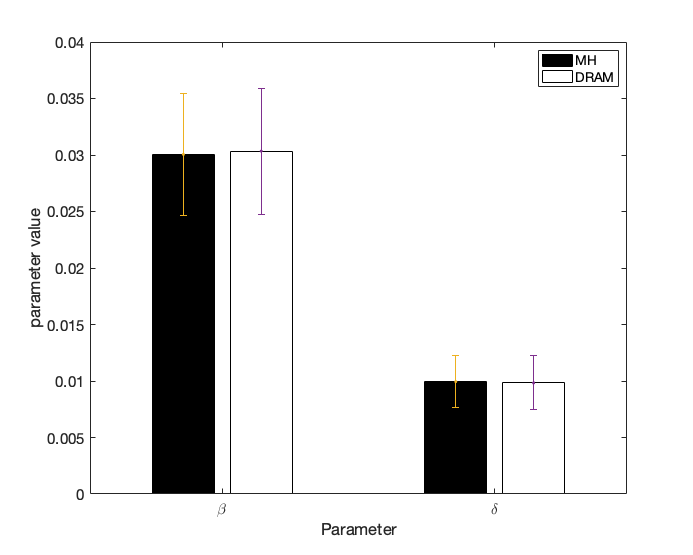
\includegraphics[width=1\linewidth]{MCMC_figs/met_lv_final/mh_dram_paramComp2.png}
  \caption{Comparison of means for $\beta$ (left) and $\delta$ (right).}
  \label{fig:12bmcmcm} 
\end{subfigure}
\caption{Comparing parameter means between the Metropolis and DRAM algorithms. Error bars were calculated using 1 standard deviation from Table \ref{tab:3mcmc}. We can see that no parameter mean values are significantly different.}
\label{fig:12mcmc}
\end{figure}
From both Table \ref{tab:3mcmc} and Figure \ref{fig:12mcmc}, we see that both algorithms are producing very similar values for each of the parameters. Figure \ref{fig:12mcmc} shows us that the means produced by each algorithm are not significantly different. This tells us both algorithms are finding the same parameter ranges in the parameter space. In order to truly compare the the performance of these two algorithms, we can compare the convergences and chain acceptance rates. While for both algorithms, we consider the chains to have converged for all parameters (Geweke $\geq 0.7$), we see that overall, the DRAM algorithm has Geweke values closer to 1. We do not have a definite reasoning for why there would be higher Geweke values for DRAM might be greater than those of the Metropolis MCMC, but we speculate that it is perhaps due to the overall sampling shapes that we saw in Figure \ref{fig:11mcmc}. With a more uniformly incremented selection of parameters, as in the DRAM algorithm, when we take the means of the first 10$\%$ and last $50\%$ of the chain, they are more likely to be very similar. On the other hand, in the Metropolis algorithm, since there is less uniformity when choosing the increments between samples, these same means are less likely to be so similar. And we can see this reflected in the difference in Geweke values. Lastly, we briefly compare the chain acceptance rates. As we mentioned before, a very general threshold for acceptance rates is around $25\%$ and is an indicator that the chain has converged and performed well. We more formally validate chain performance using the Geweke diagnostics that both chains have converged, but since the chain acceptance rate for Metropolis MCMC is significantly less than 0.25, we wonder if our algorithm is not performing as well as the DRAM algorithm.
\par We note that our statement of better performance with the DRAM algorithm is only in the context of our tutorial - that is with our specific model, burn-in period, total number of samples, likelihood functions, etc. Although we have not explored it here, increasing the number samples or tuning other parts of the Metropolis algorithm might in fact produce better results than the DRAM algorithm. The purpose of these tutorials is to help the user become more familiar with these two algorithms so that he or she can make an informed decision in choosing which algorithm to use.
\par Finally, we compare the predicted populations for hare and lynx given by parameter estimations from the Metropolis and DRAM MCMC method.
\begin{figure}[H]
    \centering
    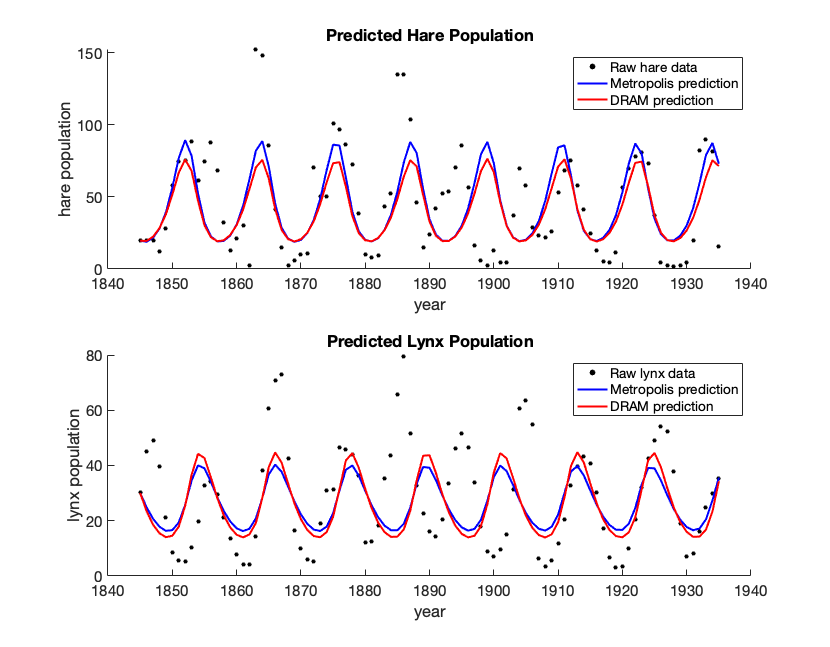
\includegraphics[width=15cm]{MCMC_figs/dram_mh_meanpredComp.png}
    \caption{Comparing mean predictions of the Metropolis and DRAM MCMC methods. Overlaid in black is the original raw hare and lynx data. Both predictions appear to capture the end behavior of the raw data, but fail to capture the starting behavior. It is difficult to visually determine which algorithm produces a better prediction.}
    \label{fig:13mcmc}
\end{figure}
While our predictions do not perfectly capture the original data, the period of each prediction is very similar to that of the original data. However, we do note some differences between the original data and each algorithm's prediction. In the lynx populations, both algorithms predict an initial decrease in population while the raw data has an increase instead. Both algorithms have a consistent period and amplitude while the raw data for both hare and lynx populations does not, thus both predictions miss a significant amount of the raw data from 1840 to around 1900. However, when the raw data becomes more consistent, around 1910 to 1940, with less variation in the period and amplitude, both predictions are able to capture these data points better. It is interesting to note that for the hare population, the Metropolis function predicts a periodic function with a greater amplitude than the DRAM algorithm and vice versa for the lynx population. But in both population predictions, they have very similar periods. 
\par While we have thus far presented several techniques for assessing algorithm performance, visual assessment of trace plots, the Geweke diagnostic, and chain acceptance rate, we base our evaluation more heavily on determining whether our algorithm has produced a prediction that captures the raw data well. In Figure \ref{fig:13mcmc}, we believe that both our algorithms have satisfactorily captured the data. We will quantify the performance more formally using root mean squared error in Table \ref{tab:4mcmc}.
\begin{table}[H]
\centering
        \begin{tabular}{c | c c}
            \cline{1-3}
            \textbf{MCMC Algorithm}  &\textbf{Hare} & \textbf{Lynx}\\
            \hline
            Metropolis & 18.16 & 31.30\\
            DRAM & 18.03 & 31.66
             \\\hline
            \hline
        \end{tabular}
    \caption{Formal comparison of the Metropolis and DRAM MCMC methods on the Lotka-Volterra system using root mean squared error (RMSE). Based on RMSE scores, there is no significant difference between the two predictions. We conclude that both the Metropolis and DRAM parameter estimations produce satisfactory populatin predictions that capture the raw data well.}
    \label{tab:4mcmc}
\end{table}
Figure \ref{fig:13mcmc} showed us that the two algorithms performed very similarly and Table \ref{tab:4mcmc} confirms this. A perfect fit of the data by the prediction would produced an RMSE score of 0. While it is difficult to formally determine an RMSE threshold for prediction performance, we consider the scores in Table \ref{tab:4mcmc} to indicate that the data was captured fairly well. In general, we would say that an RMSE score of $>$100 would indicate poor performance. While DRAM appears to perform better on the hare population prediction and the Metropolis appears to perform better on the lynx population prediction, there is no significant difference between the RMSE scores. Both Figure \ref{fig:13mcmc} and Table \ref{tab:4mcmc} suggest that both the DRAM and Metropolis MCMC algorithms can perform comparably well on this Lotka-Volterra system.
\par Perhaps it is due to the simplicity of the Lotka-Volterra model and relatively low-dimensional parameter space, that we are able to produce fairly similar predictions. However, taking note of the discrepancies between the two algorithms that we discussed early, we might assume that as a model becomes more complex and the parameter space increases exponentially (recall the curse of dimensionality), these differences may also increase. Thus, as we will parameterize the Type 1 Diabetes model in the next section, we choose to do so with the DRAM MCMC algorithm. So far this algorithm has demonstrated sufficient chain sampling (Figure \ref{fig:11bmcmcm}), convergence (Table \ref{tab:3mcmc}), and smooth distributions (Figure \ref{fig:9mcmc}).

\subsection{Parameterizing the Type 1 Diabetes Model with DRAM} \label{Parameterizing_T1D_DRAM}
We preface this section by saying that the implementation of the DRAM algorithm for the Type 1 Diabetes model is still in the process of being fine-tuned and improved. Therefore, we advise the reader to read our code and comments thoroughly and to analyze our results with some caution and skepticism.
\par We consider 10 parameters in this model, as for reasons discussed in \textbf{Sections \ref{section:NotableParameterSubset} and \ref{section:NumParamsMCMC}}, we could not parameterize all 53 parameters in the T1D ODE system. Thus we carefully chose parameters that we determined had the greatest impact on the system. The UKF algorithm found 7 parameters that seemed to vary more greatly than the others. We know from our advisors and the Shtylla et al. 2019 paper, that the eta parameters, $\alpha_{\eta}$, $\beta_{\eta}$, and $\eta$ had a great impact on diabetes onset time. Lastly, we ran our algorithm on the model for NOD mice with the apoptotic $\beta$-cell wave on. We choose these settings because all the mice in the Li et al study developed diabetes. A NOD mouse with an apoptotic $\beta$-cell wave are the biologically modelled conditions under which diabetes will occur \cite{shtylla2019mathematical}. 
\par Similar to Lotka-Volterra parameterization, we assume a Gaussian likelihood function in log base e. We implement a sum of squares function for our likelihood function (recall Step 3 of the DRAM algorithm) and so working with log values prevents our sums from increasing exponentially. Thus, the user determines a sum of squares between the model given parameter values and the original data. This sum of squares is then used to construct the acceptance criterion
\begin{equation} \label{eq:19mcmc}
lnP(D|\theta, M) = \sum_{k=1}^{N}lnP(y_k|x_k,\theta,M) = \sum_{k=1}^N SS_\theta 
\end{equation}
 We also again adopt a log-uniform prior
\begin{equation} \label{eq:20mcmc}
lnP(\theta|M) = 0
\end{equation}
The proposal distribution is determined for us in the MATLAB function \texttt{mcmcrun} using a covariance matrix. The acceptance criteria according to the \texttt{mcmcstat} library is defined as
\begin{equation} \label{eq:21mcmc}
\alpha = min(1, e^{ \lbrack {-0.5(\frac{\sum (SS_{\theta^*}-SS_{\theta^{k-1}})}{\sigma^2} + prior^*-prior^{k-1})} \rbrack}) 
\end{equation}
and thus with our assumptions simplifies to 
\begin{equation} \label{eq:22mcmc}
\alpha = min(1, e^{[ {-0.5(\frac{\sum (SS_{\theta^*}-SS_{\theta^{k-1}})}{\sigma^2}]}})
\end{equation}
Lastly, we initialize starting values and ranges for our parameters.
With all of these assumptions and initializations, we can run the DRAM MCMC algorithm and produce PDFs for each of our parameters.
\par We ran the DRAM algorithm on 4 sets of data. The first is the average acute Li mouse data that was described in the Section Problem Set Up. For comparison with this data set and UKF predictions, we also ran our algorithm on a single mouse's data set. Mouse 6 is an example of an acute mouse that we chose because of its relatively large number of data points. Lastly, we ran the algorithm using Mouse 3 and 11 (individual runs). We had visually determined that these two mice had significantly different diabetes onset times and we were interested in exploring how the algorithm's prediction would shift with this shift in onset time. 
\par In the following sections, we analyze the results of running the DRAM algorithm on the averaged data and Mouse 6 data using techniques we developed while parameterizing the Lotka-Volterra system.
\subsubsection{Parameterizing with Averaged Data}
\paragraph{Analyzing the chain}
Before jumping straight into using the results of the DRAM algorithm, we want to look at our chain for information about the algorithm's performance. We begin by looking at the trace plots of the chain for each of the parameters. We performed a burn-in period of 1,000 samples, but we only present the trace plots of the post-burn-in chain.
\begin{figure}[H]
    \centering
    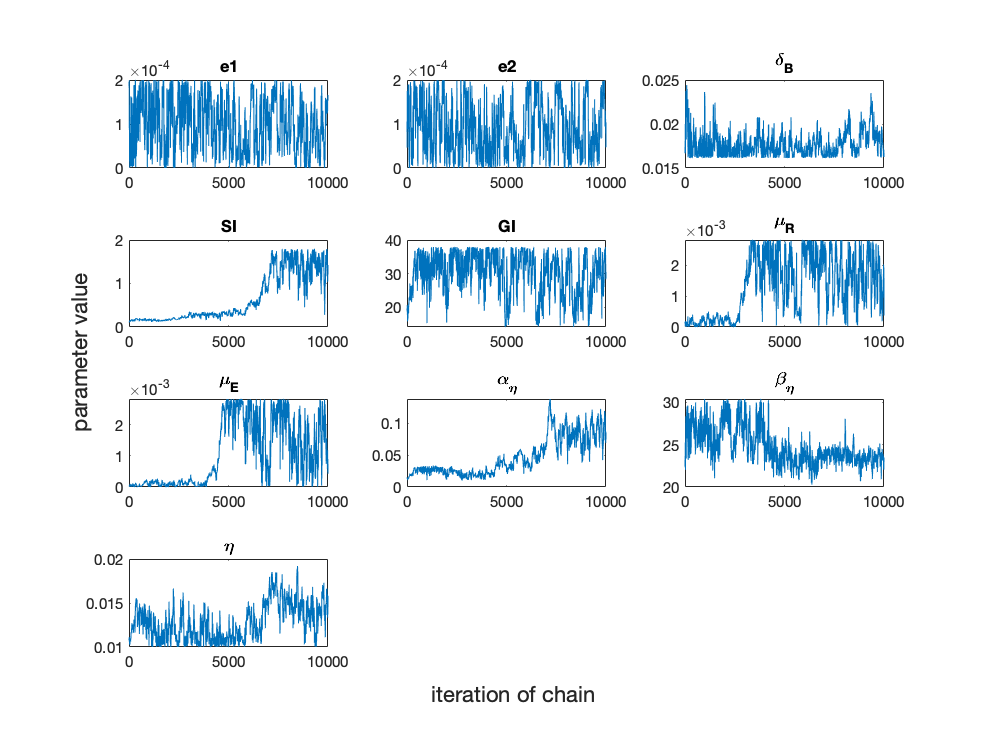
\includegraphics[width=15cm]{MCMC_figs/dram_t1d_final/final_dram_avg_traceplot.png}
    \caption{Trace plots of the sampling chain (10,000 samples) for the DRAM MCMC parameterization of the Type 1 Diabetes model on averaged Li data. Chains for each parameter are plotted separately. There are examples of good and bad chain mixing. e1 and e2 exhibit good chain mixing while $\alpha_\eta$ has poor mixing. Poor mixing is indicative of a lack of convergence.}
    \label{fig:14mcmc}
\end{figure}
We have chosen to plot each trace plot separately because the scale of the value ranges for each parameter varies greatly. Overall, there seems to be ``good" and ``bad" mixing. As we learned from looking at the chain trace plots of the Lotka-Volterra model, we would like to see a dense plot. By eye, we can see some examples of good mixing in the plots for e1, e2, and GI. Plots for $\delta_B$, $\beta_{\eta}$, and $\eta$ show moderately good mixing. The trace plots for SI, $\mu_R$, $\mu_E$, and $\alpha_{\eta}$ show a shift in parameter mean value as their mixing pattern appears to shift after a certain number of samples. We have already taken a burn-in period, but it may be that these final 4 parameters needed more time to converge. We turn to formal techniques of determining convergence to investigate the effects of the bad chain mixing.
                            
\begin{table}[H]
\centering
        \begin{tabular}{c c |c c | c c||c}
            \hline
            \textbf{Parameter} & \textbf{Initial Value} & \textbf{Mean} &  \textbf{Std} & \textbf{Geweke} & \textbf{ p-value} &\textbf{Chain Acceptance Rate}\\ 
            \cline{1-7}
            e1 & 1.0e-08 & 9.9199e-05 & 5.6117e-05 & 0.4099 &  0.68184 & \multirow{10}{*}{0.43370} \\
            e2 & 1.0e-08 & 9.2374e-05 & 5.9001e-05 & 0.2947 & 0.76824\\
            $\delta_B$ & 0.0167 & 0.017692 &  0.001341 & 0.0248 & 0.98022\\
            SI & 0.72 & 0.6345 & 0.5506  & -1.8522 & 0.063996\\
            GI & 141.4214 & 30.125 & 6.02 & 0.0436 & 0.96526\\
            $\mu_R$ & 2.0e-06 & 0.0013304 & 0.00095325 & -2.1923 & 0.028361\\
            $\mu_E$ & 2.0e-06 & 0.0010473 &  0.0010099 & -2.3090 & 0.020945\\
            $\alpha_{\eta}$ & 0.0100 & 0.04688 &  0.029704 & -1.4409 & 0.14961\\
            $\beta_{\eta}$ & 22 &  24.723 & 2.0772 & 0.2178 & 0.82762\\
            $\eta$ & 0.100 & 0.012852 &  0.0020148 & -0.1080 & 0.914
             \\\hline
                          \hline
        \end{tabular}
    \caption{Table listing results of the DRAM chain on the Type 1 Diabetes model for averaged Li data. Parameter means, standard deviations, and convergence diagnostics (Geweke) are calculated. Based on the Geweke p-values, chain has not converged for all parameters. Using a p-value of 0.05 to indicate rejection of the null hypothesis, the parameters $\mu_R$ and $\mu_E$ have statistically not converged. Parameters SI and $\alpha_\eta$ have very low p-values close to 0.05 so we are less confident in their mean values. The chain acceptance rate, while not 25\%, indicates that the algorithm is searching and accepting or rejecting candidates efficiently.}
    \label{tab:5mcmc} 
\end{table}
Unlike our Lotka-Volterra model, the chain has not converged for all of our parameters. Notably, parameters $\mu_R$ and $\mu_E$ have Geweke p-values of $< 0.05$ and thus we say that we reject the null hypothesis that the chain has converged for these parameters. Using the p-value threshold of 0.05, we say that parameters SI and $\alpha_\eta$ have converged, however their p-values are relatively low and close to 0.05 ($\sim 0.064$ and $\sim 0.15$ respectively), so we are more skeptical of their means. For the remaining parameters, e1, e2, $\delta_B$, GI, $\beta_\eta$, and $\eta$, we are confident in their mean values as based on their p-values, we fail to reject the hypothesis that the chain has converged. We note that Geweke values and their p-values may improve if we allow the algorithm to take more samples. When estimating parameters for the Lotka-Volterra model, we implemented a burn-in period of 10,000 samples and a full sampling chain of 500,000 samples. We did not do the same for the T1D model parameter estimation as the computation time increased exponentially. With a 1,000 sample burn-in period and 10,000 sample chain, our algorithm takes around 1 hour to run on a standard MacBook Air. In order to increase computational efficiency and run the DRAM algorithm for more iterations we recommend the use of a computer cluster.
\par When analyzing the chain acceptance rate of the Lotka-Volterra model, we cited literature that used an acceptance rate of around 25\% to indicate an efficient, convergent, well-performing chain \cite{convergence}. However, other authors argue that for increasingly large and complex systems, this threshold acceptance rate should also increase. In addition, they also point out that in large systems, such as the type 1 diabetes model, it is not feasible to prescribe a universal acceptance rate threshold because the interactions of the model's states and parameters will be specific to that model thereby affecting the overall acceptance rate \cite{converge_threshold}. A more in-depth investigation into the role of chain acceptance rates for large systems will be needed. For now, we are satisfied that the acceptance rate is at least significantly less than 100\%. Given these results good and bad, we are satisfied with the performance of our algorithm. We will discuss more about how we might want to determine good performance in future uses in the Discussion section.
\par Next we visualize the parameter posterior distributions.
\begin{figure}[H]
    \centering
    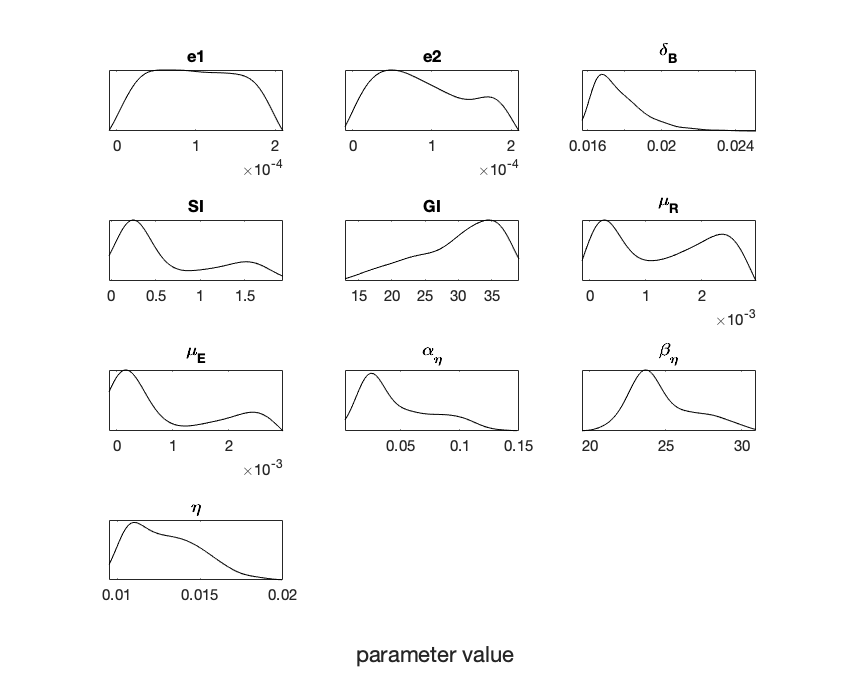
\includegraphics[width=15cm]{MCMC_figs/dram_t1d_final/jul10_avg_run1(noIC)_acute_NOD_waveOn_lietal_den.png}
    \caption{DRAM parameter distributions for 14 Type 1 Diabetes parameters for averaged Li data. Some parameters exhibit bimodal distributions. Specifically, $\mu_R$ and $\mu_E$ appear to have bimodal distributions. Recall from Table \ref{tab:5mcmc} that these parameters had very low Geweke values, this indicates that algorithm was not able to determine a global maximum for each parameter as is apparent in their distributions.}
    \label{fig:15mcmc}
\end{figure}
It is not useful for us to try to formally classify these distributions however, we can see some familiar shapes. Parameters $\delta_B$, $\alpha_eta$, and $\beta_{\eta}$ appear log-normal-ish. Others like e1 and e2 appear almost uniform. Lastly, we make note of the parameters whose distributions seem to be bimodal: SI, $\mu_R$, and $\mu_E$ are the most pronounced, but an argument could be made for the bimodal pattern in some of the other parameters. It is also important to note that the chain had not converged for both $\mu_R$ and $\mu_E$ according to their p-values in Table \ref{tab:5mcmc} and SI had a p-value of $\sim 0.064$, very close to the 0.05 threshold. The lack of convergence that we saw statistically is corroborated with these bi-modal distributions. We hypothesize that the algorithm was not able to determine a global maximum for SI, $\mu_R$, and $\mu_E$ and thus sampled in two ranges resulting in the bi-modal distribution and lack of convergence. However, it is important to remember that some parameters may not have a global maximum and instead have multiple local maxima, that is they may have more than one optimal range of values (it will likely depend on a parameter's individual interaction with another parameter). Altogether, these distributions appear relatively smooth, which unfortunately does not give us any other clues for the lack of convergence that we saw in Table \ref{tab:5mcmc}.
\paragraph{Working with the distributions}
Now that we have an understanding of the performance of our chain, we can explore the predicted results. We first look at model prediction that uses DRAM's mean parameter values.
\begin{figure}[H]
\centering
\begin{subfigure}{.7\textwidth}
    \centering
    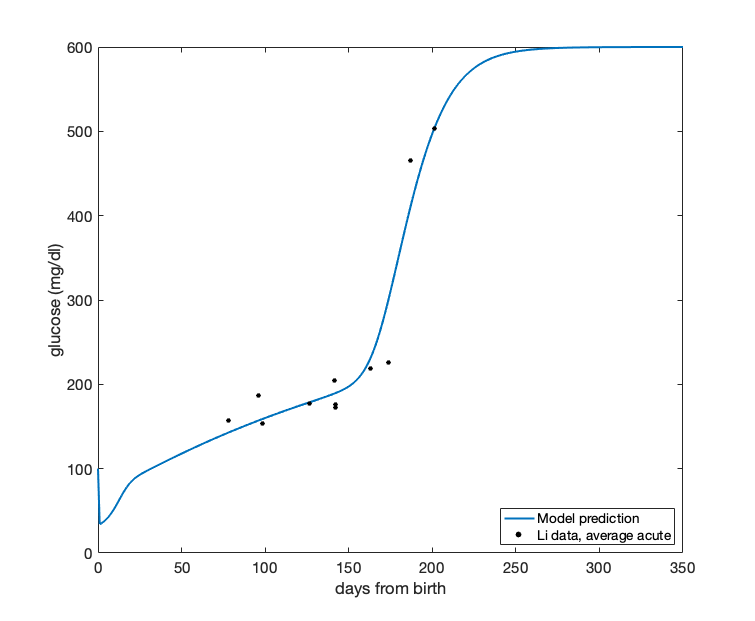
\includegraphics[width=1\linewidth]{MCMC_figs/dram_t1d_final/jul10_avg_run1(noIC)_acute_NOD_waveOn_lietal_meanpred.png}
    \caption{Predicted Glucose model plotted using mean DRAM parameter values.}
    \label{fig:17amcmc}
\end{subfigure}
\begin{subfigure}{.7\textwidth}
    \centering
    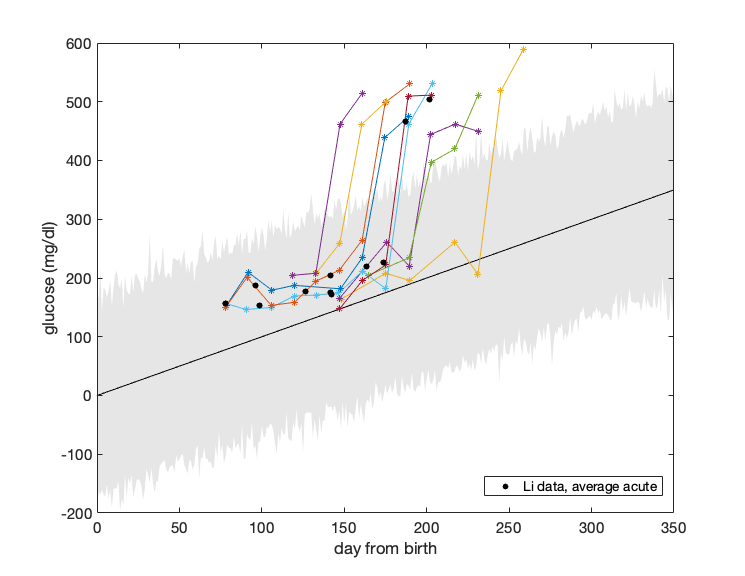
\includegraphics[width=1\linewidth]{MCMC_figs/dram_t1d_final/95_CI_avg.png}
    \caption{Predicted glucose model with $95\%$ probability range plotted with averaged acute data and the 9 acute Li et al. mice.}
    \label{fig:17bmcmc}
\end{subfigure}
\caption{Plotting glucose predictions. In 23(a), the averaged acute Li data is plotted over the prediction. The prediction appears to capture the original data fairly well. We see the characteristic acute mouse slow steady increase and then spike of glucose indicating diabetes onset. In 23(b), the prediction does not appear to capture the original data well as not all the data points are captured within the $95\%$ probability range. It is unclear to us why these two predictions produce such different results.}
\label{fig:17mcmc}
\end{figure}
In Figure \ref{fig:17bmcmc}, we present a figure analogous to the Lotka-Volterra predictions in Figures \ref{fig:5mcmc} and \ref{fig:10mcmc}. In addition to the 95$\%$ prediction range, we plot the original 9 acute mice data and the averaged acute data. Although a majority of the points are captured within the $95\%$ probability range, we are unsure why the overall trend of these predictions is linear. It is important to note that we did not write the code that plots Figure \ref{fig:17bmcmc}, so it is difficult for us to tune the plot. The reason that we believe that there are plotting issues that figures is that when we plot Figure \ref{fig:17amcmc}, the prediction is actually fairly good. This is something to be investigated in the future.). In Figure \ref{fig:17mcmc}, we only plot one prediction of the glucose state using the DRAM mean parameter values. From this figure, it seems that this prediction is capturing the original data quite well and we are satisfied with the overall trend of the prediction. 

\subsubsection{Parameterizing with Mouse 6 Data}
We chose to run the DRAM algorithm on a single mouse because we want to see the results using only raw data. Recall that in the averaged data, we had to make some assumptions about the overall time frame of our data. With mouse 6 data, we can avoid over-generalization and making assumptions. 
\paragraph{Analyzing the chain}
We begin by looking at the trace plots of the chain for each of the parameters. We performed a burn-in period of 1,000 samples, but we only present the trace plots of the post-burn-in chain.
\begin{figure}[H]
    \centering
    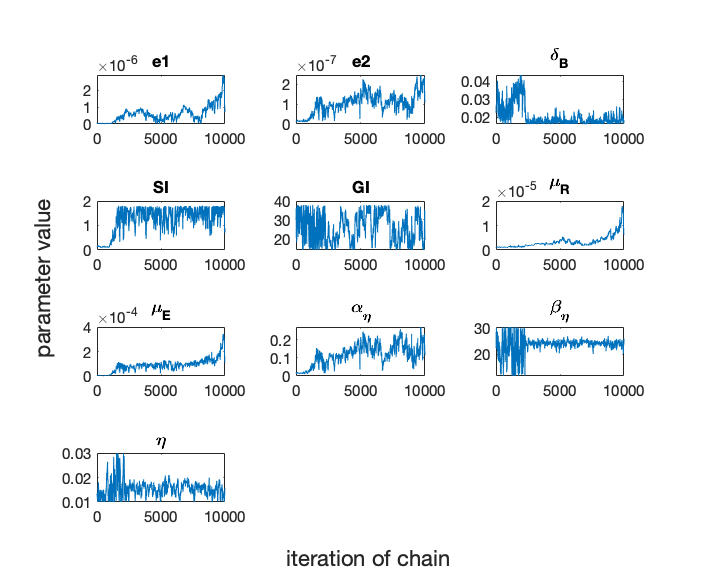
\includegraphics[width=15cm]{MCMC_figs/dram_t1d_final/final_dram_mouse6_traceplots.png}
    \caption{Trace plots of the sampling chain (10,000 samples) for the DRAM MCMC parameterization of the Type 1 Diabetes model on mouse 6 only. Chains for each parameter are plotted separately. We see a mixture of good and poor chain mixing. GI exhibits good mixing while $\mu_R$ and $\mu_E$ exhibit bad mixing. This indicates that chain has not converged for parameters with poor mixing.}
    \label{fig:18mcmc}
\end{figure}
Immediately we see that there is an overall lack of good mixing. Parameter GI seems to be the closest to having good mixing. It is interesting to see now that we can determine some of the parameters that will not have converged. Parameters $\delta_B$, $\beta_{\eta}$, and $\eta$ have pretty dramatic shifts in means during the 10,000 iterations. Recalling the definition of Geweke's diagnostic, these 3 parameters are unlikely to have similar means for the first 10\% and last 50\% of their chain, thus we know that they have not converged. However, these convergences are likely better, in comparison to parameters whose trace plots look like e1, e2, $\mu_R$, $\mu_E$, and $\alpha_{\eta}$. These barely look like classic chain trace plots and their means are almost constantly changing. We turn to formal techniques of determining convergence to investigate the effects of the poor chain mixing.
\begin{table}[H]
\centering
        \begin{tabular}{c c|c c | c c ||c}
            \hline
            \textbf{Parameter} & \textbf{Initial Value} & \textbf{Mean} &  \textbf{Std} & \textbf{Geweke} & \textbf{p-value} &\textbf{Chain Acceptance Rate}\\ 
            \cline{1-7}
            e1 & 1.0e-08 & 5.9625e-07 & 4.8352e-07 & -2.2691 & 0.023261 & \multirow{10}{*}{0.541} \\
            e2 & 1.0e-08 & 1.0391e-07 &  5.029e-08 & -2.2122 & 0.026956\\
            $\delta_B$ & 0.0167 & 0.020498 &  0.0057686 &  0.5394 & 0.58958\\
            SI & 0.72 &  1.2582   &  0.50705  & -2.2012 & 0.027721\\
            GI & 141.4214 &  25.949 &  7.0361 & 0.1279 & 0.89823\\
            $\mu_R$ & 2.0e-06 & 3.3264e-06 & 2.5351e-06 & -1.8527 & 0.063928\\
            $\mu_E$ & 2.0e-06 &  8.8867e-05 & 5.2077e-05 & -2.4567 & 0.014021\\
            $\alpha_{\eta}$ & 0.0100 & 0.11996 & 0.057717 & -2.1727 & 0.029801\\
            $\beta_{\eta}$ & 22 &  23.507 & 2.8037 & -0.1665 & 0.86778\\
            $\eta$ & 0.0100 & 0.015418 &  0.0031396 & -0.2313 & 0.81708
             \\\hline
                          \hline
        \end{tabular}
    \caption{Table listing results of the DRAM chain on the Type 1 Diabetes model for mouse 6 only. Parameter means, standard deviations, the convergence diagnostic (Geweke), and Geweke p-values are calculated. Based on the Geweke p-values, the chain has not converged for all parameters. In particular, parameters e1, e2, SI,  $\mu_E$, and $\alpha_\eta$ have p-values $< 0.05$ thus we reject the hypothesis that the chain has converged for these parameters. The chain acceptance rate seems to be a reasonable value as it is not significantly larger than 50\% and is much less than 100\%.}
    \label{tab:6mcmc}
\end{table}
Compared with the parameters from the DRAM parameter estimation using the averaged data, in Table \ref{tab:6mcmc} we have significantly less convergence (Table \ref{tab:5mcmc}). Parameters e1, e2, SI,  $\mu_E$, and $\alpha_\eta$ all have p-values $< 0.05$ and thus we must reject the null hypothesis that the chain has converged for these parameters. The parameter $\mu_R$ has a p-value of $\sim 0.064$ which is close to our threshold of 0.05, thus we are less confident in the accuracy of the mean of this parameter. For the remaining parameters, $\delta_B$, GI, $\beta_\eta$, and $\eta$, we fail to reject our null hypothesis and say that the chain has converged for these parameters. The chain acceptance rate does not give us much information regarding chain performance but for now, we are satisfied that the acceptance rate is not significantly larger than 50\% and is much less than 100\%. Thus, we believe our chain is giving a satisfactory parameterization. So far, the algorithm has not performed as well on the Mouse 6 data than on the averaged data.
\par Next we visualize the parameter posterior distributions.
\begin{figure}[H]
    \centering
    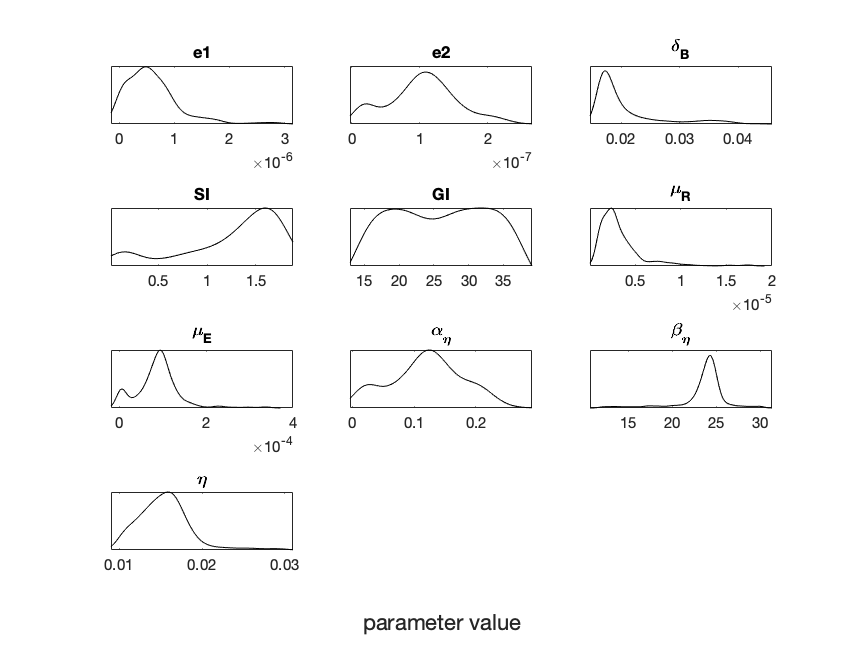
\includegraphics[width=15cm]{MCMC_figs/dram_t1d_final/jul10_mouse6_run1(noIC)_acute_NOD_waveOn_lietal_den.png}
    \caption{DRAM parameter distributions for 14 Type 1 Diabetes parameters for mouse 6. For some parameters, like $\mu_E$ and $\alpha_\eta$, the results of Table \ref{tab:6mcmc} are confirmed with bimodal distributions and lack of smoothness. We conclude that for some parameters, the algorithm was unable to determine the best range of values for that parameter.}
    \label{fig:19mcmc}
\end{figure}
Overall these distributions look drastically different than those in Figure \ref{fig:15mcmc} (we will do a more formal comparison of parameter means in a subsequent section). In looking at the distributions of the parameters for which the chain did not converge, e1, e2, SI,  $\mu_E$, and $\alpha_\eta$, we see that the distributions for e2, SI, $\mu_E$, and $\alpha_\eta$ appear to have some degree of bi-modal behavior. This is most pronounced in the PDFs of e2 and $\mu_E$. These bi-modal behaviors indicate and the lack of convergence that we saw in Table \ref{tab:6mcmc} indicates that the DRAM algorithm was struggling to determine a global maximum. It appears that it might have found two ranges of values with higher probability.
\paragraph{Working with the distributions}
Next we analyze the performance of the DRAM algorithm by assessing the fit of the glucose prediction that we can produce from the estimated parameter values.
\begin{figure}[H]
\centering
\begin{subfigure}{.7\textwidth}
    \centering
    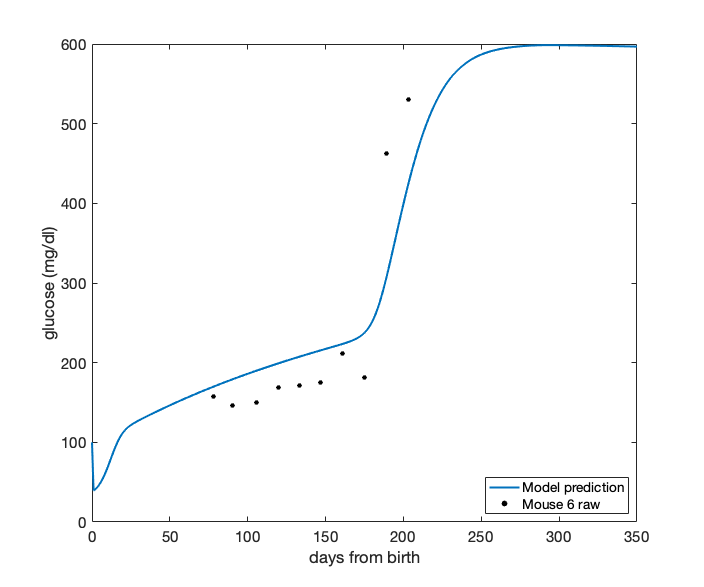
\includegraphics[width=1\linewidth]{MCMC_figs/dram_t1d_final/jul10_mouse6_run1(noIC)_acute_NOD_waveOn_lietal_meanpred.png}
    \caption{Predicted Glucose model plotted using mean DRAM parameter values. }
    \label{fig:mouse6amcmc}
\end{subfigure}
\begin{subfigure}{.7\textwidth}
    \centering
    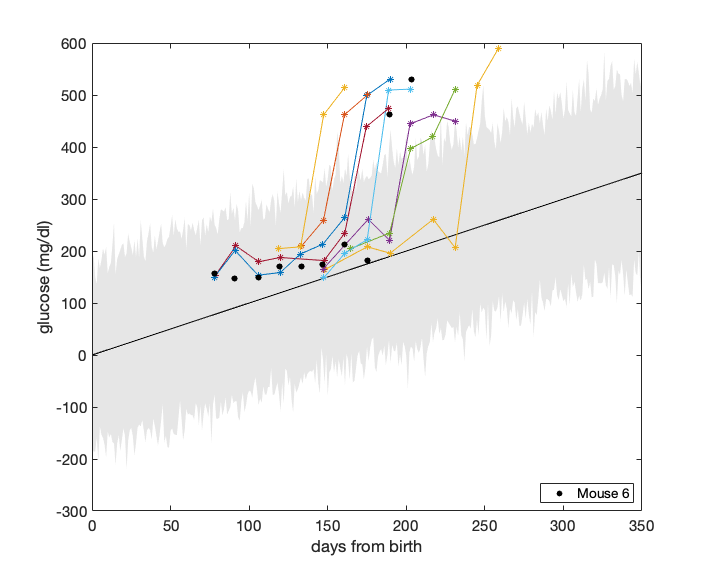
\includegraphics[width=1\linewidth]{MCMC_figs/dram_t1d_final/95_CI_mouse6.png}
    \caption{Predicted glucose model with $95\%$ probability range plotted with the 9 acute Li et al. mice.}
    \label{fig:mouse6bmcmc}
\end{subfigure}
\caption{Plotting glucose predictions from DRAM parameterization using Mouse 6 data. In 26(a), the Mouse 6 data is plotted over the prediction. Despite poor chain performance for some parameters, the prediction seems to capture the data fairly well. In 23(b), the prediction does not appear to capture the any of the individual mice well as not all the data points are captured within the $95\%$ probability range. It is unclear to us why these two predictions produce such different results.}
\label{fig:mouse6mcmc}
\end{figure}
We similar results from our parameterization using averaged data in Figure \ref{fig:mouse6bmcmc}. In addition to the 95$\%$ prediction range, we plot the original 9 acute mice data and the averaged acute data. Although a majority of the points are captured within the $95\%$ probability range, we are unsure why the overall trend of these predictions is linear. From Figure \ref{fig:mouse6amcmc}, it seems that our prediction is capturing the general trend of the original data, but it is not capturing the raw data as well as the prediction in Figure \ref{fig:17mcmc}. We are satisfied with the overall trend of the prediction, however, we are cautious in trusting the parameter values because a majority of our parameter did not show convergence (Table \ref{tab:6mcmc}). Nevertheless, we in the next section we compare the overall mean predictions and parameter values.
\subsubsection{Evaluating the DRAM Algorithm}
Our final step in assessing the DRAM algorithm is to evaluate and compare our parameter estimates from both the averaged acute and the Mouse 6 data sets. We do an evaluation both visually and formally using a mean-squared error score and finally, we compare the actual mean values of the parameters. 
\par Although we only present the full results from 2 different data sets used to parameterize the type 1 diabetes model, we have run the DRAM algorithm on 2 additional individual Mice, 3 and 11 in order to compare the role of the data set. We begin by comparing differences in parameters for which the chain has converged between parameterizations using the different data sets.
% 3: 0.8484    0.7691    0.9104    0.0710    0.4664               0.6179    0.1840    0.0242    0.8388    0.9860

% 11: 0.9249    0.7804    0.5049    0.0655    0.9074              0.0940    0.9985    0.0288    0.9937    0.7456
\begin{table}[H]
\centering
        \begin{tabular}{c|c c|c| c c}
            \hline
            \textbf{Parameter} & \textbf{Data Set} &  \textbf{Geweke p-value} & \textbf{Parameter} & \textbf{Data Set} &  \textbf{Geweke p-value} \\
            \cline{1-6}
            \multirow{4}{*}{e1} & Mouse 3 & 0.8484 & \multirow{4}{*}{$\mu_R$} & Mouse 3 & 0.6179\\
            & Mouse 6 & 0.023261 & & Mouse 6 & 0.063928\\
            & Mouse 11 & 0.9249 & & Mouse 11 & 0.0940\\
            & Averaged & 0.68184 & & Averaged & 0.028361 \\\hline
            \multirow{4}{*}{e2}  & Mouse 3 & 0.7691 & \multirow{4}{*}{$\mu_E$} & Mouse 3 & 0.1840\\
            & Mouse 6 & 0.026956 & & Mouse 6 & 0.014021\\
            & Mouse 11 & 0.7804 & & Mouse 11 & 0.9985\\
            & Averaged & 0.76824 & & Averaged & .020945\\\hline
            \multirow{4}{*}{$\delta_B$} & Mouse 3 & 0.9104 & \multirow{4}{*}{$\alpha_\eta$} & Mouse 3 & 0.0242\\
            & Mouse 6 & 0.58958 & & Mouse 6 & 0.029801\\
            & Mouse 11 & 0.5049 & & Mouse 11 & 0.0288\\
            & Averaged & 0.98022 & & Averaged & 0.14961 \\\hline
            \multirow{4}{*}{SI} & Mouse 3 & 0.0710 & \multirow{4}{*}{$\beta_\eta$} & Mouse 3 & 0.8388 \\
            & Mouse 6 & 0.027721  & & Mouse 6 & 0.86778\\
            & Mouse 11 & 0.0655 &&  Mouse 11 & 0.9937\\
            & Averaged & .063996 & & Averaged & 0.82762\\\hline
            \multirow{4}{*}{GI} & Mouse 3 & 0.4664  & \multirow{4}{*}{$\eta$} & Mouse 3 & 0.9860\\
            & Mouse 6 & 0.89823 & & Mouse 6 & 0.861708\\
            & Mouse 11 & 0.9074  & &Mouse 11 & 0.7456\\
            & Averaged & 0.96526 & &Averaged & 0.914\\\hline
             \hline
        \end{tabular}
    \caption{Table comparing the Geweke p-values for DRAM parameter estimates using 4 different data sets. Based on the p-values, the chain has converged for the parameters $\delta_B$, GI, $\beta_\eta$, and $\eta$ in all 4 parameterizations. For the rest of the parameters, there is a mixture of convergence and non-convergence between data sets.}
    \label{tab:pvalComp}
\end{table}
In Table \ref{tab:pvalComp} we compare the Geweke p-values from individual DRAM parameter estimations using 4 different data sets for each of the parameters. We note that we see only consistent convergence across data sets for the parameters $\delta_B$, GI, $\beta_\eta$, and $\eta$. All the other parameters have at least one data set for which the chain did not converge. For example, for the parameter e1, the chain has converged in the Mouse 3, Mouse 11, and Averaged data sets, yet it failed to converge for Mouse 6 as we see a p-value of $\sim 0.023$ which is $< 0.05$. While the p-values for e1 are fairly high for the Mouse 3, Mouse 11, and Averaged data sets (0.8484, 0.9249, and 0.68184 respectively), for other parameters like SI, the p-values are consistently low for all the data sets. While for SI, statistically we fail to reject the null hypothesis that the chain has converged in Mouse 3, Mouse 11, and the Averaged data sets, all 4 p-values are fairly close to the 0.05 threshold. Thus, we are less confident in the mean values of SI from each DRAM parameter estimation.
\begin{figure}[H]
    \centering
    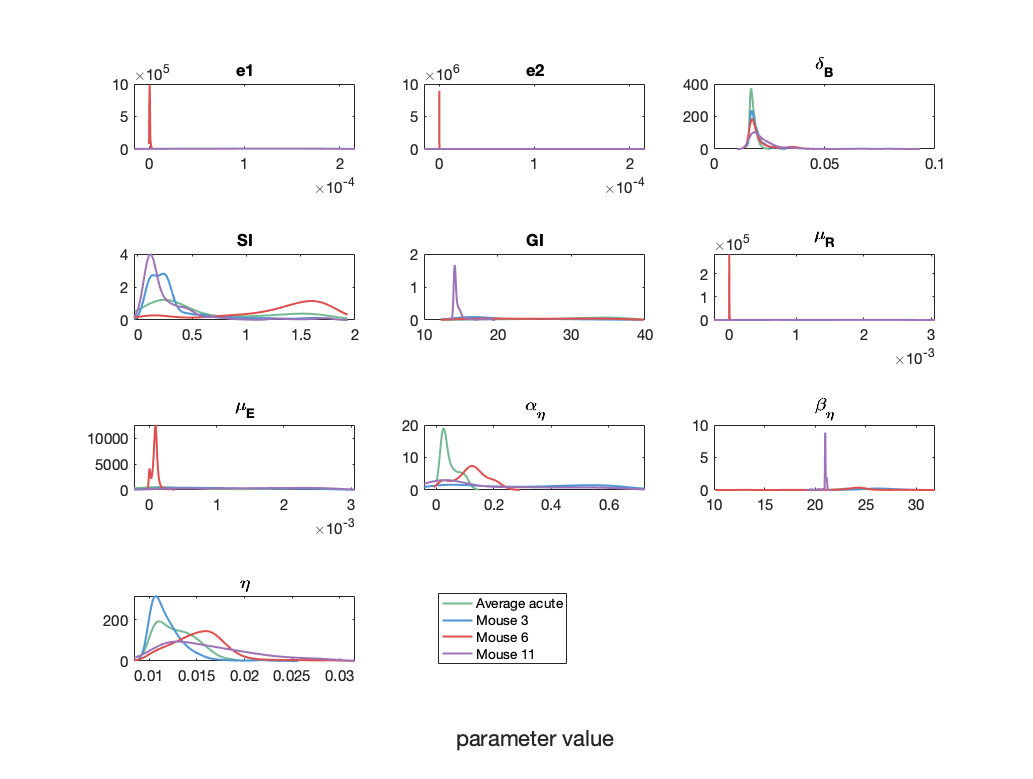
\includegraphics[width=18cm]{MCMC_figs/dram_t1d_final/PDFs_3_6_11_avg.png}
    \caption{Comparison of parameter posterior distributions from DRAM parameterizations performed on Mice 3, 6, 11 data and averaged acute data. Some parameter distributions appear to differ very significantly: e1, e2, GI, $\mu_R$, $\mu_E$, $\beta_eta$. These differences are somewhat expected as we are fitting parameterizations using different data sets. Other parameter distributions appear more similar: $\delta_B$ and $\eta$.}
    \label{fig:overlaiddist_t1d}
\end{figure}
From Figure \ref{fig:overlaiddist_t1d}, we can see that there is quite a lot of variation between distributions of parameters between parameterizations on the different data sets. Notably, for parameters e1, e2, $\mu_R$, and $\mu_E$, the Mouse 6 parameterization have distinctly ``spiked" distributions with significantly greater mean values. The same is true for the Mouse 11 parameterization for parameters GI and $\beta_\eta$. We are unsure of the cause of these thin lone spikes, however we can reason that perhaps the algorithm was unable to sample a larger range for these parameter values. It is interesting to note that parameters e1, e2, $\mu_R$, and $\mu_E$ also have very low Geweke values (Table \ref{tab:6mcmc}). These low convergence diagnostic values in combination with the spiked distribution further indicate that the algorithm appears to have gotten stuck in a small range of values and was likely rejecting a majority of the candidates (and alternatives). We are pleased to see that for parameters $\delta_B$, SI, $\alpha_\eta$, and $\eta$, the distributions between parameterizations are more similar. In particular, the distributions for $\delta_B$ are very similar in shape.
\par Next, we visually compare the resulting glucose predictions below.
\begin{figure}[H]
    \centering
    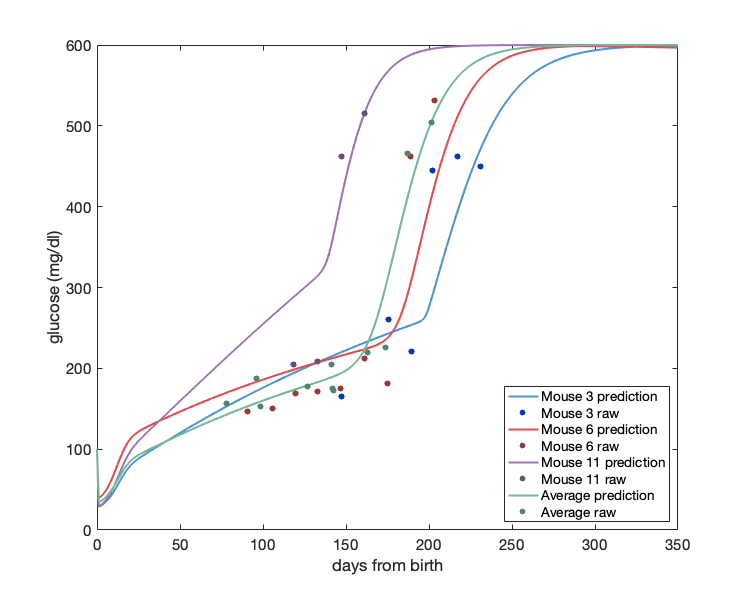
\includegraphics[width=15cm]{MCMC_figs/dram_t1d_final/comp_3_6_11_avg_finalfig.png}
    \caption{Comparing glucose predictions of DRAM parameterizations for mouse 3, mouse 6, mouse 11, and averaged acute data. Through the differences in pivot points and slopes of the starting behaviors, we can see that the data the algorithm begins with is important in determining the final model prediction, particularly in determining the diabetes onset time.}
    \label{fig:21mcmc}
\end{figure}
The overall shapes and behaviors are similar between runs. The largest differences are in the starting behavior slopes and diabetes onset times. We attribute most of these differences to the differences in the original data used during the individual parameterizations. For example, mouse 11's data has the earliest onset time and consequently its prediction has the earliest onset time. The same can be said for mouse 3 which has the latest onset time in both the raw data and prediction. This figures tells us that data seems to play a key role in determining the final model predictions and thus the final parameter values. For a more formal comparison, we calculate the root mean squared error for each prediction using its respective raw data.
\begin{table}[H]
\centering
        \begin{tabular}{c | c}
            \cline{1-2}
            \textbf{Data Set}  &\textbf{RMSE}\\
            \hline
            Mouse 3 & 75.2\\
            Mouse 6 & 66.8\\
            Mouse 11 & 66.3\\
            Average & 30.7
             \\\hline
            \hline
        \end{tabular}
    \caption{Comparison of glucose predictions produced by DRAM using original data from mouse 3, 6, 11 and averaged acute data. RMSE was calculated individually. Based on the RMSE scores, the algorithm captures the averaged data best.}
    \label{tab:7mcmc} 
\end{table}
The RMSE scores tell us that the prediction based on averaged data seems to capture the original data (average acute) the best, although the individual mouse predictions each seem to be performing comparably. While it seems we have a clear best prediction, it is less clear why the averaged data parameterization produced the best results. Perhaps it is because Mice 3 and 11 do not have as many data points. We hypothesize that the number of data points affects the likelihood sum of squares function (recall Step 6d of the DRAM algorithm). Let's say we have 5 data points and we calculate the sum of squares function with a prediction of the ODE model. But we are only able to compare the prediction at these 5 data points and thus, even if the prediction does a poor job of capturing the data (resulting in a large sum of squares), this value might not be as great as if we calculated the sum of squares using the same prediction for 100 data points. Recall from Section \ref{The_Acceptance_Criteria} that a larger sum of squares increases the probability of accepting a specific parameter set candidate. Therefore, with fewer data points, our likelihood function and subsequently our acceptance criterion may not provide an acceptance-rejection threshold that will allow us to find the optimal parameter values.
\par Lastly, we are curious to see how much the final parameter mean values from each run of the algorithm differ. We present the following 3 figures that compare means of mouse 6 and the averaged data parameterization only as these have produced the best results according to Figure \ref{fig:21mcmc} and Table \ref{tab:7mcmc}. Error bars were based on the standard deviations of each parameter mean (these can be found in Tables \ref{tab:5mcmc} and \ref{tab:6mcmc}). We have separated the parameter comparisons because of the difference in magnitude as can be observed on the y-axes. Lastly, we note that we choose not to visually compare the parameters e1, e2, $\mu_R$, $\mu_E$, and $\alpha_\eta$ because their means differed by more than a magnitude of 10. This is due to 1) difficulty in side-by-side comparison and 2) if parameter values differ by such a great magnitude, it is reasonable to say that they are significantly different without plotting their error bars.
\begin{figure}[H]
\begin{subfigure}{.5\textwidth}
    \centering
    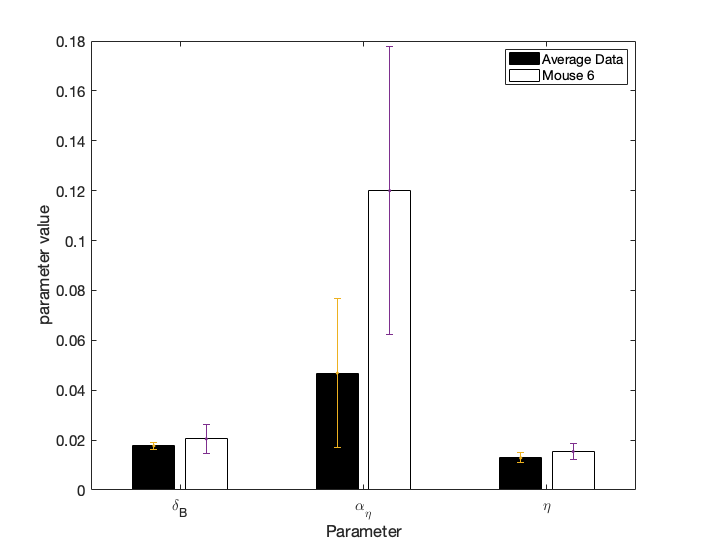
\includegraphics[width=.8\linewidth]{MCMC_figs/dram_t1d_final/mouse6_avg_paramComp1.png}
    \caption{Mean comparison for parameters $\delta_B$, $\alpha_{\eta}$, and $\eta$. Error bars were created using 1 standard deviation in \textbf{Tables \ref{tab:6mcmc} and \ref{tab:5mcmc}}. There does not appear to be a statistical difference between means of these 3 parameters.}
    \label{fig:22mcmc}
\end{subfigure}
\begin{subfigure}{.5\textwidth}
    \centering    
    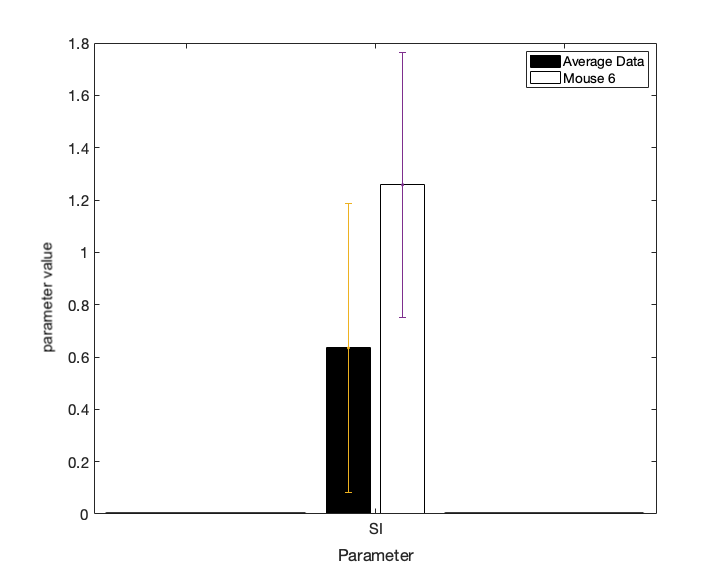
\includegraphics[width=.8\linewidth]{MCMC_figs/dram_t1d_final/mouse6_avg_paramComp_SIONLY.png}
    \caption{Mean comparison for parameters SI. Error bars were created using 1 standard deviation in \textbf{Tables \ref{tab:6mcmc} and \ref{tab:5mcmc}}. There does not appear to be a statistical difference between the means of SI.}
    \label{fig:23mcmc}
\end{subfigure}
\begin{center}
\begin{subfigure}{.5\textwidth}
    \centering
    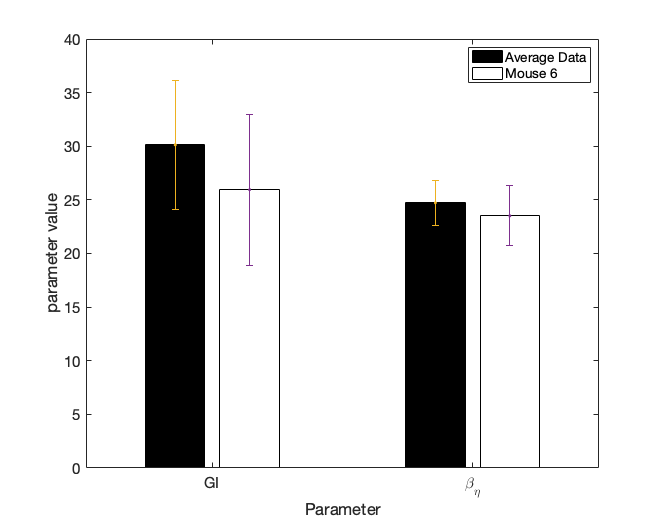
\includegraphics[width=.8\linewidth]{MCMC_figs/dram_t1d_final/mouse6_avg_paramComp2.png}
    \caption{Mean comparison for parameters GI, $\beta_{\eta}$. Error bars were created using 1 standard deviation in \textbf{Tables \ref{tab:6mcmc} and \ref{tab:5mcmc}}. There does not appear to be a statistical difference between the 2 parameters.}
    \label{fig:24mcmc}
\end{subfigure}
\end{center}
\end{figure} 


From these comparisons, we note that 6 out of our our 10 total parameter means are not significantly different between data sets. This gives us some more insight into the differences between convergent parameters in both runs of the algorithms. For example, the 3 common converged parameters between averaged and mouse 6 predictions are $\delta_B$, GI, $\beta_{\eta}$, and $\eta$, these parameters seem to be the most similar in value, therefore we can feel relatively confident in their respective mean values. On the other hand, SI is the only parameter that we have compared (Figure \ref{fig:23mcmc}) that did not converge for either run of the algorithm, we are therefore much more suspicious of these values. 

\paragraph{Takeaways}
Overall, we are satisfied with the DRAM's performance in estimating parameters for the Type 1 diabetes model. We are most impressed with the parameter estimation for the averaged data, as the DRAM seems to perform the best on this data set. As we will discuss in the following sections, we continue to estimate parameters for the T1D model and finally compare the performance of each algorithm.


\section{Particle Swarm Optimization}\label{PSO_SECT}

Particle Swarm Optimization (PSO) is a global optimization algorithm that falls within the class of evolutionary algorithms. Similarly to MCMC, it functions by iteratively and stochastically proposing solutions to an optimization problem, judging the quality of each solution proposed by a user-defined metric. As a meta-heuristic, PSO is widely applicable (CITE). For the purpose of parameterizing biological models, the optimization problem in question is finding the parameter set that produces a solved system that most closely fits an empirical data set. This is accomplished by lending an appropriate function for minimization to the PSO algorithm, known as the \emph{objective function} (CITE). The objective function is what is numerically minimized to judge how closely a system solved with the proposed parameters fits the data set in question.
\par PSO is worthy of investigation for parameterization of biological models due to its computational efficiency and minimal reliance on design parameters. This makes implementation of PSO for parameter fitting straight-forward and generalizable. In a similar vein, PSO is also significantly less dependent on an initial set of values than either MCMC or Kalman Filters. This is due to the use of many points by the swarm. PSO is also derivative-free, meaning that an objective function need not be differentiable. In addition to reducing computational complexity, this opens up many possibilities for the evaluation of how well a given parameter set fits observed data (CITE). Finally, PSO is highly appropriate to parameterize models with a large number of parameters. Because optimizing $p$ parameters requires a search space of dimension $p$, the ability to PSO to run easily in parallel makes this task more manageable and efficient (CITE). 
\par In this section, we begin by explaining the algorithm behind PSO in Section \ref{PSO_alg}. We then tutorial its implementation in the case study of the Lotka-Volterra model in Section \ref{PSO_LV}. Moving then to the more complex T1D system in Section \ref{PSO_T1D}, we show a more refined implementation of PSO, as well as show how its versatility makes it a useful tool for validation. 

\subsection{Algorithm}\label{PSO_alg}
PSO's algorithmic development by Kennedy and Eberhart in 1995 was based on work done by zoologists and sociobiologists simulating the movement of flocks of birds. A model in and of itself, PSO was meant to capture the social interactions between birds within the flock. Each bird has a level of autonomy, yet the flock moves as a whole; their movement relies of their own knowledge, known as \emph{individual knowledge}, and the swarm's knowledge, known as \emph{social knowledge}. Kennedy and Eberhart aimed to replicate this idea of individual and collective movement by representing each bird in the flock with a simple software agent, referred to as a \emph{particle}. 

\par Put metaphorically, as a flock of birds flies, all birds are searching for food. Each bird knows where the best food source it has seen is, and it can listen to the squawks of others to determine their findings. If another bird has found a better food source than this bird has ever seen, it will likely change its flight path to investigate what that other bird has found. Otherwise, it will continue to explore, but also keep in mind the best food source it has found so far, drifting towards that point. All in all, as this process progresses, this leads to the flock localizing to one area, the location with the optimum food. Putting this mathematically, the algorithm is as follows:

% INSERT PSO ALG DESC HERE %
\subsection{General Implementation} \label{PSO_Imp}
MATLAB includes a built-in implementation of PSO in the Global Optimization Toolbox, known simply as \texttt{particleswarm}. It is straightforward in its setup and allows for reasonable customization of the design parameters. Though the specification of many of the following components of PSO are optional in the MATLAB implementation, and left to their default values in our work, they are described here. 
\subsubsection{Objective Function}
The objective function is a necessary part of PSO, and must be supplied to \texttt{particleswarm} as an anonymous function in MATLAB. It directs how the coordinates of parameter space visited by the particles should be used. 
\subsubsection{Swarm Size}
\subsubsection{Iterations}
\subsubsection{Velocity Components}
\subsubsection{Acceleration Coefficients}
\subsubsection{Topology}


\subsection{Lotka-Volterra Implementation} \label{PSO_LV}
\subsubsection{Specifications}
\subsubsection{Results}

\subsection{T1D Implementation} \label{PSO_T1D}
\subsection{Specifications}
\subsubsection{Results}
\subsubsection{PSO as Validation}




%\section{Kalman Filter Overview} \label{KF_SECT}
\section{Kalman Filters} \label{KF_SECT}
\subsection{A General Overview of Kalman Filtering}
Kalman Filters (KF) fall under the umbrella of Machine Learning models, however are additionally an example of a mechanistic model, meaning that it allows us to gain an understanding of the individual, inner workings of complex systems. Moreover, unlike MCMC's, which are used on already fully obtained data sets, Kalman Filters can be adjusted as new data is brought in \cite{ChowFerrer}. This makes Kalman Filters unique in that they can operate in real time as well. Rather than making predictions using an entire dataset at once, KFs improve and evolve as more datapoints are assessed. To use a KF, the system must be in a discretized state space form \cite{SimonHaykinText}. To do this, one must identify two sets of variables: latent states and observables.\\

Latent states are the set of variables that one is interested in estimating, which can include values such as a population count or model parameters. On the other hand, observables are a set of data which has been measured from the system and is the only piece of information known about the system at a particular time point \cite{ChowFerrer}. \\

Additionally, Kalman Filters are helpful due to their ability to quantify the noise associated with a system. This is achieved through both process and measurement noise. Process noise describes outside forces and situations which, as a result of their actions, affect states in the model. Measurement noise, on the other hand, accounts for the fact that tools to gather observable data may be inherently flawed, and thus some level of noise is associated with the values they produce \cite{ChowFerrer}. In order to gather a holistic, high level understanding of Kalman Filters, consider the example of a car driving down a street.\\

Assume that one observes a car at time $t$ traveling at a velocity of $Y$ m/s at a position of $X$ m from an observed starting point, as seen in Figure \ref{fig:Car_Example}. In order to estimate what the car's velocity will be at time $t+1$, one may choose to utilize a Kalman Filter. Assuming that the position at time $t+1$ can be measured to be $Z$ m with a device such as a ruler, this position thus is the observable, while the velocity is a latent state. However, since the tool is flawed, measurement noise is added in as well. If we assume that while this is occurring, a force of $W$ Newtons pushes from above the car, this would now become a source of process noise. Having all of this information, one is now capable of applying a KF to estimate the velocity of the car at time $t+1$.\\

\begin{figure}[H]
    \centering
    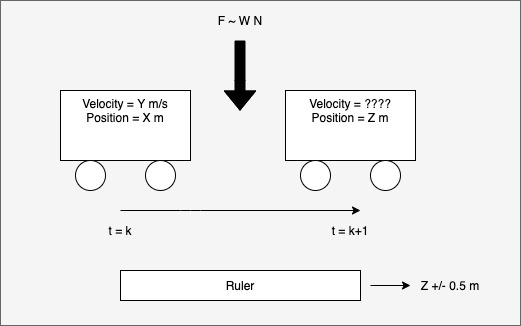
\includegraphics[width=15cm]{Kalman_Filter_Images/Cart_Example.jpg}
    \caption{A visualization of utilizing a Kalman Filter to estimate the velocity of a car. Here, the latent state is the velocity while the observable is the distance.}
    \label{fig:Car_Example}
\end{figure}

As stated earlier, Kalman Filters operate in discrete time, state space models, meaning that input and output variables are being related to one another through a system of ODEs at known time points. Thus, we must have knowledge about the system to the extent that we know the structure of the ODEs, although as we'll see, there are formats of the Kalman Filter in which it is not necessary to know the parameter values. Having both an understanding of the ODEs and the observable data, we can now introduce the the projection and update steps, the two of which drive the KF algorithm and are visualized in Figure \ref{fig:UKF_TwoSteps}. 
%{The simplest use of Kalman Filters is for state estimation, which we will describe in the following sections. Although our eventual goal is to implement parameter estimation, since parameter estimation is based on the foundation of state estimation, it is easier to understand if you first have a general understanding of state estimation. As a result of this, we will introduce  parameter estimation later on.%} 

\begin{figure}[H]
    \centering
    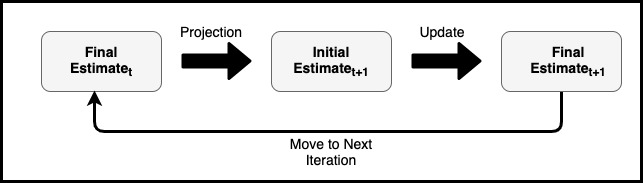
\includegraphics[width=15cm]{Kalman_Filter_Images/Simple_UKF_Flow.jpg}
    \caption{The two steps of the Kalman Filter algorithm. First, we use knowledge of the system to create an initial prediction, following which observable data is produced to produce final estimates.}
    \label{fig:UKF_TwoSteps}
\end{figure}

\textbf{Projection Step}: The first step of the KF relies only on knowledge of the system. Having an estimate of latent states at time $t$, we use our knowledge of the system to predict the states at time $t + 1$, known as the prior estimate \cite{SimonHaykinText} \cite{GoveHollingerDual}.\\

\textbf{Update Step}: Having a prior estimate, we can now bring in the observable data. By seeing how the prediction we made in the Projection Step compares to the observable data, we now update our predictions and states \cite{GoveHollingerDual}. This is now our posterior estimate \cite{SimonHaykinText}, and becomes the set of states that are projected forward to produce the prior estimate for time $t+2$. We continue this loop as long as new data is coming in, continously improving results as more data arrives. \\
\\


\subsection{Introduction to Kalman Filters}
    Please note that all notation and equations in this section and section \ref{section:UKF_Theory} are adapted from \cite{VanMereChapter} and \cite{SimonHaykinText}, two sources we have found very helpful in guiding our understanding of Kalman Filters.
    \subsubsection{Different Types of Kalman Filters}
    Multiple formulations of Kalman Filters exist for different types of systems. When a system is linear, one may use the standard Linear Kalman Filter. However, once the system becomes nonlinear this is no longer feasible. If the nonlinear system may be accurately linearized with first order Taylor approximations, the Extended Kalman Filter (EKF) may be used. The theory for the EKF is based around the first order Taylor approximation. However, if the nonlinear system  is not easily linearized, it is recommended to use the Unscented Kalman Filter (UKF) \cite{VanMereChapter}. Due to the inability of complex ODE systems to be accurately approximated with first order Taylor approximations, we will focus on the Unscented Kalman Filter here.
    
    \textbf{A Note on Parameter Estimation} The general UKT, which we will describe in the following sections is built for state estimation purposes. However, the UKF can also be used for parameter estimation, which is the context in which it will be used when describing its implementation. Specifically, we will be using the UKF to estimate states and parameters at the same time via the Joint and Dual methods, described in section \ref{section:Parameter_Estimation}.
    
    
    
    \subsubsection{Process and Measurement Equations}
    The Unscented Kalman Filter is used to estimate the states of a nonlinear system. The system, set up as a state space model, is described by the process and measurement equations \cite{SimonHaykinText}. The process equation, describing the transition of the latent states from time $k$ to time $k+1$ is formulated as
    \begin{equation}
    x_{k+1} = F_{k+1,k}(x_k) + q_k, 
    \end{equation}
    where $x_{k}$ is the vector of states at time $k$, $x_{k+1}$ is the vector of states at time $k+1$, $F$ is the non-linear transition function that takes the state from time $k$ to time $k+1$, and $q_k$ is the process noise \cite{SimonHaykinText}. $F$ and $q_k$ are assumed to be known quantities. The latent states are the variables that we are trying to estimate. The Measurement equation, describing the relationship between observed data points and the unknown states, is 
    \begin{equation}
    y_k = H_k(x_k) + r_k,  
    \end{equation}
    where $y_k$ is the vector of the observables, $H$ is a (possibly) nonlinear function that relates the states to the observables, and $r_k$ represents the measurement noise \cite{SimonHaykinText}. Often times, only some sort of algebraic combination of states can be observed. For example, if the latent state is simply $x$, we may only be able to observe $3x^2$. Thus, the purpose of $H$ is to relate the actual observed value, $3x^2$ to the latent state $x$.\\
    \\
    $H$ and $r_k$ are assumed to be known in the Measurement equation. 
    \subsubsection{Set up of the Noise}
    The above system of equations relies on both process and measurement noise. The vector $q_k$, which follows the same dimensions as the state vector in order to apply one noise value to each state, describes the process noise and is multivariate Gaussian with mean 0 and covariance described by 
    \begin{equation}
    E[q_{n}q_{k}^T] = \Bigg\{\begin{tabular}{l}
    $Q_k$\ for\ n = k  \\
    0   for \ $n \neq k$
    \end{tabular}.
    \end{equation}
    
    Similarly, $r_k$ describes the measurement noise and is Gaussian with mean 0 and covariance described by 
    \begin{equation}
    E[r_{n}r_{k}^T] = \Bigg\{\begin{tabular}{l}
    $R_k$\ for\ n = k  \\
    0   for \ $n \neq k$
    \end{tabular}. 
    \end{equation}
    
    
    Both of these covariance matrices will play a role in the UKF calculations. Furthermore, it is important to note that our system assumes white, additive noise. If we have a system where the noise is not additive, the Kalman Filter equations must be altered, which can be seen in \cite{VanMereChapter}. 
    
    \subsubsection{Unscented Transformation}
    Developed in response to the shortcomings of Kalman Filters on nonlinear systems, The Unscented Kalman Filter is formulated around the Unscented Transformtation (UT) \cite{JulierPaper}. The UT is used to understand the distribution of a random variable after a nonlinear transformation has been applied to it \cite{JulierPaper}. 
    \\
    To understand the distribution of a random variable post a nonlinear transformation, the UT creates a set of \textbf{sigma vectors} meant to capture points in the distribution in an ideal, deterministic fashion \cite{JulierPaper} \cite{VanMereChapter}. Consider random variable $v$, i.e.
    
    \begin{equation}
    v = \begin{bmatrix} v_1\\ v_2\\v_3\\.\\.\\.\\v_L\end{bmatrix},
    \end{equation}
    
    with dimensions $L$ x $1$. Additionally, consider a different random variable $z$ that is some function of $v$ such that $z = f(v)$. Also assume that the distribution of $v$ has mean $\bar{v}$ and covariance $P_v$. To understand the distribution of the nonlinear transformation y, we create an $L$ x $2L+1$ matrix $\chi$ of 2$L$ + 1 sigma vectors as follows:
    \begin{equation} \label{eq:UT_1}
    \chi_0 = \bar{v}
    \end{equation}
    \begin{equation} \label{eq:UT_2}
    \chi_i = \bar{v} + (\sqrt{(L + \lambda)P_v})_i \ i = 1 ... L
    \end{equation}
    \begin{equation} \label{eq:UT_3}
    \chi_i = \bar{v} - (\sqrt{(L + \lambda)P_v})_{i - L} \ i = L + 1 \  ...  \ 2L + 1.
    \end{equation}
    The number 2$L$+1 gives us one vector at the mean, or expectation, of the random variable and $L$ vectors above and below the mean. As stated above, $L$ is the dimension of $v$ which means it is number of states in our system. The subscript $i$ refers to the $i$th columns in the matrix square root of the term $(\sqrt{(L + \lambda)P_v})$.\\

    Here, $\lambda$ is a final scaling parameter defined as $\alpha^2(L + k) - L$, where $\alpha$ is a scaling parameter that represents the spread of vectors around $\bar{v}$. $k$ is a secondary scaling parameter, set to either 0 or $3-L$, whereas $\alpha$ takes on a value between 10e-4 and 1 \cite{VanMereChapter}. It is crucial to note that this is a form of \textbf{deterministic} scaling. In many sampling schemes, sampling is done \textbf{randomly} from a distribution. However, here our goal is to choose points in equal intervals and in equal quantities of either side of the mean, $\bar{v}$. The purpose of this is so that we may be certain that sigma points accurately capture the spread of a distribution. With random sampling, if only choosing a small amount of points, we can make no guarantees about the distribution of these points. Thus, exact equations are given for how the sigma vectors should be chosen. \\
    \\
    Once $\chi$ has been calculated, the sigma vectors are then sent through the nonlinear function $f$ to create vectors $Z_i$. This is done as follows:
    \begin{equation}
    Z_i = f(\chi_i) \ \ i = 0,...,2L.
    \end{equation}
    
    Now, by weighting these output vectors $Z_i$ in a deterministic fashion, we can calculate a mean and covariance in order to understand our new distribution \cite{VanMereChapter}. In order to do this, we create the following weights, where $W^{(m)}$ are weights corresponding to calculating the mean and $W^{(c)}$ is used to calculate our covariance:
    \begin{equation} \label{eq:Weights_1}
    W_0^{(m)} = \lambda/(L + \lambda),
    \end{equation}
    \begin{equation} \label{eq:Weights_2}
    W_0^{(c)} = \lambda/(L + \lambda) + (1 - \alpha^2 + \beta),
    \end{equation}
    \begin{equation} \label{eq:Weights_3}
    W_i^{(m)} = W_i^{(c)} = 1/(2(L + \lambda)) \ i = 1 ... 2L.
    \end{equation}
    Here, $\beta$ holds prior knowledge about the distribution (for Gaussian $\beta = 2$ is used) \cite{VanMereChapter}. We can see that the sigma point that represents the mean is given more weight than the others. Now the mean and covariance can be calculated:
    \begin{equation}
     \bar{z} \approx \sum_{i = 0}^{2L} W_i^{(m)} Z_i,
    \end{equation}
    \begin{equation}
    P_z \approx \sum_{i = 0}^{2L} W_i^{(c)}(Z_i - \bar{z})(Z_i - \bar{z})^T.    
    \end{equation}
    Understanding this mean and covariance will be useful in creating our prior estimates in the UKF method.
    \\
    
    For a visual representation of the importance of the UT, see Figure \ref{fig:UT_Diagram_Custom}.
    \begin{figure} [H]
    \centering
    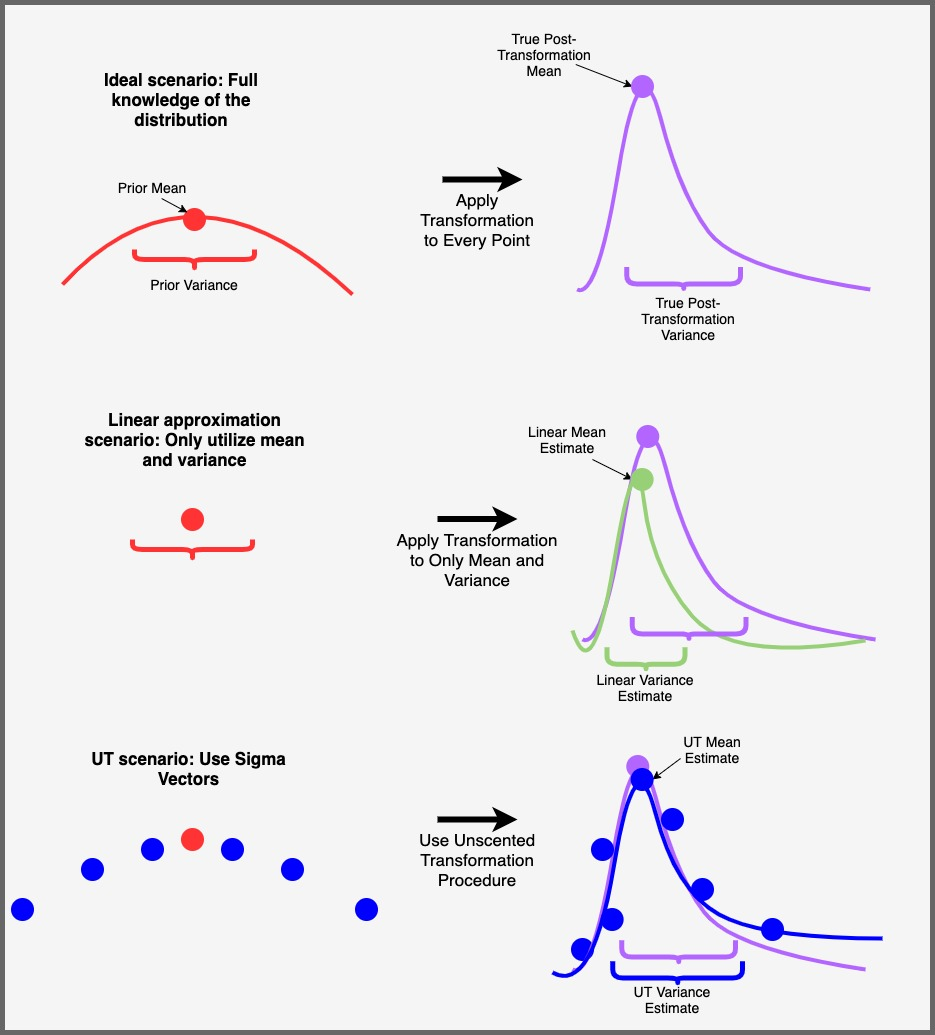
\includegraphics[scale = .5]{Kalman_Filter_Images/Unscented_Transformation_Diagram.jpg}
    \caption{A comparison of 3 techniques to understand the distribution of a transformation of a random variable. At the top, we see an ideal schema where we have full knowledge of a distribution and can transform every point to understand the true mean and covariance of the RV post-transformation, as seen in purple. In the second row, we linearize the transformation and only transform the mean and variance. However, this does not produce a good approximation, which is shown in green. Lastly, we use the UT to deterministically choose sigma vectors that are transformed and then weighted to more accurately capture the new mean and variance, as shown in blue.}
    \label{fig:UT_Diagram_Custom}
    \end{figure}
    
    Figure \ref{fig:UT_Diagram_Custom} visualizes the importance of the Unscented Transformation. In an ideal scenario, one has full knowledge of a RV's distribution and can thus apply the transformation to every single possible point to understand the new mean and variance. However, we often need ways to approximate the nonlinear transformation. One naive solution is to linearize the transformation and only transform the mean and variance, however this results in not as accurate of a fit \cite{VanMereChapter}. The solution to this issue is the Unscented Transformation. By deterministaclly choosing the blue sigma vectors, applying the transformation, and then weighting these transformed vectors, we are able to much more closely capture the actual mean and variance of the RV post-transformation. As a result, sigma vectors play a key role in the inner-workings of the Unscented Kalman Filter.\\
    
    Having a theoretical understanding of the UT, we can now discuss the specifics of the UKF algorithm.
    
    \subsection{Theory of the Unscented Kalman Filter} \label{section:UKF_Theory}
    
    \subsubsection{Notation}
    Before delving deeper into the process of using a Kalman Filter, it is important to establish the notation that will be used throughout. This notation is adapted from \cite{SimonHaykinText} and \cite{VanMereChapter}.
    \paragraph{States Notation}
    For our states, we first have $\hat{x}_0$ for our initial posterior estimate. Next, we notate our prior estimate as $\hat{x}_k^-$ and our posterior estimate, following the Update Step, as $\hat{x}_k$. Then, we have analogous notation for the states covariance. Namely, we start with $P_0$, have a prior estimate of $P_k^-$, and then a posterior covariance of $P_k$.
    \paragraph{Observables Notation}
    We must define similar notation for our observables. Here, we have a prior estimate $\hat{y}_k^-$, but instead of a posterior estimates, we have the \emph{actual} observable value $y_k$. Using these two values, we also define the error, or \emph{innovation}, as:
    \begin{equation}
    \tilde{y}_k = y_k - \hat{y}_k^-.    
    \end{equation}
    Then, we once again have a covariance matrix, but this time for the innovation, $P_{\tilde{y}_k}$. This is the basis of the notation, however more will be introduced as necessary in the following sections, and a full guide can be found in Table \ref{table:KF_Notation}.
    
    \subsubsection{Initialization}
    The initial states vector $x_0$ and the initial covariance matrix between the states, $P_0$, are needed to initialize the UKF. To create these initial guesses some prior knowledge of the states and their plausible ranges is necessary. Assuming this information is available, one may initialize with:
    \begin{equation}
    \hat{x}_0 = E[x_0],
    \end{equation}
    and initial covariance matrix:
    \begin{equation}
    P_0 = E[(x_0 - \hat{x}_0)(x_0 - \hat{x}_0)^T].
    \end{equation}
    \cite{VanMereChapter}
    When working with real data, one is not likely to have a full understanding of the states' distribution. Thus, a first guess will suffice and may be tuned throughout working with the UKF, as will be discussed in section \ref{KF_General_Implementation}.  
    \subsubsection{Projection Step}
    Now, we proceed to do the projection portion of the algorithm. Having chosen a set of sigma points via equations \ref{eq:Weights_1}, \ref{eq:Weights_2}, and \ref{eq:Weights_3} , we now project them in time by applying the transition matrix to each point in the vector $\chi_{k-1}$:
    \begin{equation}
    \chi_{k|k-1} = F(\chi_{k-1}).
    \end{equation}
    It is important to note that here $\hat{x}_{k-1}$ plays the role of $\bar{v}$ in equations \ref{eq:UT_1}, \ref{eq:UT_2}, and \ref{eq:UT_3}.
    Next we calculate a prior prediction of the state $\hat{x}_k^-$ with:
    \begin{equation}
    \hat{x}_k^- = \sum_{i = 0}^{2L} W_i^{(m)} \chi_{i, k|k-1}.
    \end{equation}
    Similarly we can calculate a prior covariance $P_k^-$ by using our weights as well as the process noise:
    \begin{equation}
    P_k^- = \sum_{i = 0}^{2L} W_i^{(c)} [\chi_{i, k|k-1} - \hat{x}_k^-][\chi_{i, k|k-1} - \hat{x}_k^-]^T + Q.
    \end{equation}
    We can see that the calculation of $\hat{x}_k^-$ and $P_k^-$ are both \emph{applications of the Unscented Transformation} as we created, transformed, and weighted sigma vectors. Next, we apply the UT transformation to understand our observables with:
    \begin{equation}
    Y_{k|k-1} = H[\chi_{k|k-1}].
    \end{equation}
    This allows us to know calculate a prior estimate of the observables $y_k^-$ by utilizing:
    \begin{equation}
    \hat{y}_k^- = \sum_{i=0}^{2L} W_i^{(m)} Y_{i,k|k-1}.
    \end{equation}
     Once again, we have made use of the \emph{UT transformation} here by passing our sigma vectors through $H$ this time, as opposed to $F$ as before.
    \subsubsection{Update Step}
    Having created prior estimates for both states and observables, we now proceed to the update step where the observed data is brought in \cite{VanMereChapter}. \\
    
    We begin by calculating the covariance matrix $P_{\tilde{y}_k, \tilde{y}_k}$, which is the covariance matrix for the error between the projected and actual values of the observables. \\
    
    Moreover, this calculation takes into account the measurement noise through $R$:
    \begin{equation}
    P_{\tilde{y}_k, \tilde{y}_k} = \sum_{i=0}^{2L} W_i^{(c)} [Y_{i,k|k-1} - \hat{y}_k^-][Y_{i,k|k-1} - \hat{y}_k^-]^T + R. 
    \end{equation}
    Next we need a covariance between our states and observables, which is calculated by:
    \begin{equation}
    P_{{x}_k,{y}_k} = \sum_{i=0}^{2L} W_i^{(c)} [\chi_{i,k|k-1} - \hat{x}_k^-][Y_{i,k|k-1} - \hat{y}_k^-]^T.
    \end{equation}
    At this point, we have sufficient information to calculate the \textbf{Kalman Gain}, a crucial term in the UKF algorithm. The Kalman Gain is used to weight the error between the predicted value and the observed value of $x_k$ in order to update the filter's prior predictions. A larger Kalman Gain will give more weight to the error, resulting in a larger correction and a smaller Kalman Gain will give less weight to the error, resulting in a smaller correction. The Kalman Gain is also used to adjust the covariance matrix $P_k$ and is calculated through \cite{VanMereChapter}:
    \begin{equation}
    K_k = P_{x_k, y_k} P_{\tilde{y}_k, \tilde{y}_k}^{-1}. 
    \end{equation}
    Calculation of the Kalman Gain allows us to calculate our posterior estimates of both the states, $\hat{x}_k$, and covariance, $P_k$ \cite{VanMereChapter}. For the states the following equation is used
    \begin{equation}
    \hat{x}_k = \hat{x}_k^- + K_k(y_k - \hat{y}_k^-). 
    \end{equation}
    And for the covariance we use:
    \begin{equation} \label{eq:27ukf}
    P_k = P_k^-  - K_k P_{\tilde{y}_k, \tilde{y}_k} K_k^T.
    \end{equation}
    We can see that both equations function by adjusting our prior prediction through use of the Kalman Gain.\\
    \\
    After having gone through the update step, the next data point would be brought in and we would return to the Projection Step once more.
    \subsubsection{Summary}
    A flow chart depicting one iteration of the entire UKF process is found in figure \ref{fig:UKF_Theory_FlowChart}. To summarize, our goal is to begin with a set of sigma points chosen in a deterministic fashion and arrive at the posterior estimates for the states and covariance. This is done in two main sections, the Projection Step, whose quantities are shaded in red, and the Update Step, displayed in blue.
    
    \begin{figure} [H]
    \centering
    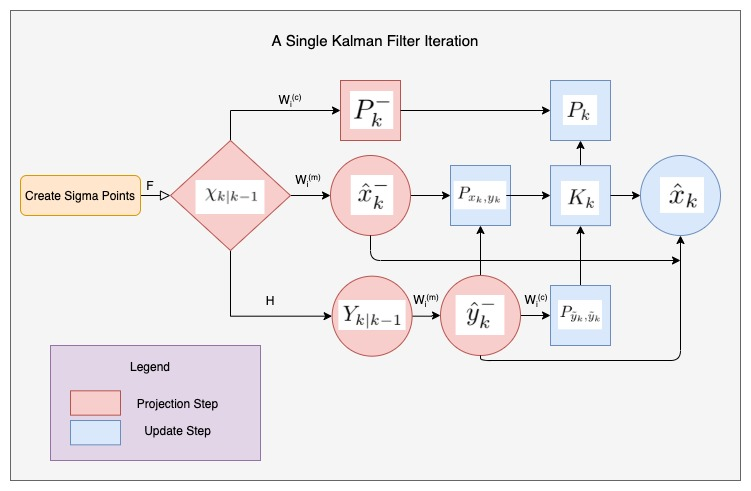
\includegraphics[scale = 0.6]{Kalman_Filter_Images/UKFFlowDiagram.jpg}
    \caption{A flow chart depicting one iteration of the UKF process. The sigma points are shaded in yellow, the intermediate steps in red, the Kalman gain in green, and the posterior estimates in blue.}
    \label{fig:UKF_Theory_FlowChart}
    \end{figure}
    
    \subsubsection{Stability and Divergence Issues}
    When utilizing the UKF, it is important to consider the issue of positive definitiness of the covariance matrix $P_k$. If this matrix becomes non-positive definite, the filter can experience severe divergence issues due to invalid covariance matrices, which can occur as a result of the update made in equation \ref{eq:27ukf}. This then can lead the filter to diverge \cite{SimonHaykinText}. \\
    
    The solution to the issue lies in using the \textbf{Cholesky factorization} \cite{SimonHaykinText}.
    \\
    
    At every iteration of the Kalman Filter, one must perform the following step:
    \begin{equation}
    P_k = {P_k}^{1/2} {P_k}^{T/2},
    \end{equation}
    where ${P_k}^{1/2}$ is the \textbf{Cholesky factor} and is in lower-triangular form, and ${P_k}^{T/2}$ is the Cholesky factor's transpose \cite{SimonHaykinText}. Here, $P_k$ is now the product of a square matrix and its transpose, which is \textbf{guaranteed to be positive definite}. In order to find the Cholesky factor, a function such as Matlab's \emph{chol} (https://www.mathworks.com/help/matlab/ref/chol.html) can be used. By using this approach, one will have a better chance of maintaining the stability of the Kalman Filter across iterations. \\

    
\begin{tcolorbox} [breakable, enhanced]

\textbf{\underline{The Unscented Kalman Filter Algorithm With Additive Noise}} 
\begin{enumerate}
    \item Initialize $\hat{x}_0 = E[x_0]$ or with best guess.
    \item Initialize $P_0 = E[(x_0 - \hat{x}_0)(x_0 - \hat{x}_0)^T]$ or with best guess.
    \item For each incoming data point perform the following:
    \begin{enumerate}
        \item Projection Step
        \begin{enumerate}
            \item Create Sigma Points 
            \begin{itemize}
                \item  $\chi_0 = \bar{x}$
                \item $ \chi_i = \bar{x} + (\sqrt{(L + \lambda)P_x})_i \ i = 1 ... L $
                \item $ \chi_i = \bar{x} - (\sqrt{(L + \lambda)P_x})_{i - L} \ i = L + 1 \  ...  \ 2L + 1 $
            \end{itemize}
            \item Project Sigma Points forward with
            $$\chi_{k|k-1} = F(\chi_{k-1})$$
            \item Calculate prior state estimate
            $$ \hat{x}_k^- = \sum_{i = 0}^{2L} W_i^{(m)} \chi_{i, k|k-1}$$
            \item Calculate prior covariance estimate 
            $$ P_k^- = \sum_{i = 0}^{2L} W_i^{(c)} [\chi_{i, k|k-1} - \hat{x}_k^-][\chi_{i, k|k-1} - \hat{x}_k^-]^T + Q$$
            \item Project observables forward with 
            $$Y_{k|k-1} = H[\chi_{k|k-1}]$$
            \item Calculate prior observable estimate 
            $$\hat{y}_k^- = \sum_{i=0}^{2L} W_i^{(m)} Y_{i,k|k-1}$$
        \end{enumerate}
        \item Update Step
        \begin{enumerate}
            \item Calculate innovation covariance 
            $$P_{\tilde{y}_k, \tilde{y}_k} = \sum_{i=0}^{2L} W_i^{(c)} [Y_{i,k|k-1} - \hat{y}_k^-][Y_{i,k|k-1} - \hat{y}_k^-]^T + R$$
            \item Calculate state and observable covariance
            $$ P_{{x}_k,{y}_k} = \sum_{i=0}^{2L} W_i^{(c)} [\chi_{i,k|k-1} - \hat{x}_k^-][Y_{i,k|k-1} - \hat{y}_k^-]^T$$
            \newpage
            \item Calculate Kalman Gain
            $$K_k = P_{x_k, y_k} P_{\tilde{y}_k, \tilde{y}_k}^{-1}$$
            \item Calculate posterior state estimate
            $$\hat{x}_k = \hat{x}_k^- + K_k(y_k - \hat{y}_k^-)$$
            \item Calculate posterior state covariance
            $$P_k = P_k^-  - K_k P_{\tilde{y}_k, \tilde{y}_k} K_k^T$$
            \item Perform Choletsky Factorization
            $$P_k = {P_k}^{1/2} {P_k}^{T/2}$$
        \end{enumerate}
        \item Set $k$ to $k + 1$ and proceed to next data point
        
        \end{enumerate}
    \end{enumerate}


\end{tcolorbox}
  
    
\begin{table}[H]
  \begin{center}
    \label{tab:table1}
    \begin{tabular}{c|c} % <-- Alignments: 1st column left, 2nd middle and 3rd right, with vertical lines in between
      \textbf{Parameter} & \textbf{Definition}\\
      \hline
      \textbf{$\hat{x}_0$} & Initial state guess\\
      \hline
      \textbf{$P_0$} & Initial state covariance guess\\
      \hline
      \textbf{$\chi$} & Matrix of sigma vectors\\
      \hline
      \textbf{$L$} & Number of states\\
      \hline
      \textbf{$\lambda$} & Scaling parameter\\
      \hline
      \textbf{$F$} & Transition matrix/function\\
      \hline
      \textbf{$H$} & Measurement matrix/function\\
      \hline
      \textbf{$W$} & Unscented Transformation weights\\
      \hline
      \textbf{$Q$} & Process noise covariance\\
      \hline
      \textbf{$R$} & Measurement noise covariance\\
      \hline
      \textbf{$\hat{x}_k^-$} & Prior state estimate\\
      \hline
      \textbf{$\hat{y}_k^-$} & Prior observable estimate\\
      \hline
      \textbf{$P_k^-$} & Prior state covariance estimate\\
      \hline
      \textbf{$\tilde{y}_k$} & Innovation\\
      \hline
      \textbf{$P_{\tilde{y}_k, \tilde{y}_k}$} & Innovation covariance\\
      \hline
      \textbf{$P_{x_k, y_k}$} & State and observable covariance\\
      \hline
      \textbf{$K_k$} & Kalman Gain\\
      \hline
      \textbf{$\hat{x}_k$} & Posterior state estimate\\
      \hline
      \textbf{$P_k$} & Posterior state covariance estimate
    \end{tabular}
    \caption{Full set of notation used in the Kalman Filter equations, adapted from \cite{SimonHaykinText} and \cite{VanMereChapter}.}
    \label{table:KF_Notation}
  \end{center}
\end{table}
    
    
\subsection{Parameter Estimation - Dual versus Joint} \label{section:Parameter_Estimation}
Up to this point the UKF has been described in the sense of performing state estimation, where all the parameters of the ODE model are known. However, there are often scenarios, such as the Lotka-Volterra and T1D systems, where model parameters are unknown and need to be estimated. In order to do so, we can use the Joint and Dual UKF methods. \cite{VanMereChapter}.

    \subsubsection{Joint}
    The Joint UKF algorithm is done very similarly to a standard state-estimation UKF. However, the parameters of the model, call them $\theta$, are now appended to the state vector to make one large state vector. In essence, the parameters become states to be estimated. Thus, given states $x$ and parameters $\theta$, our latent states vector becomes a concatenation of the two. In order to implement this, we treat the transition function related to the parameters as an identity since our goal is to estimate constant parameter values. 
    \subsubsection{Dual}
    In the Dual UKF, two UKFs are run in parallel, one for the states and one of the parameters. The estimates for the parameters at a specific time point are then fed into the state filter, and the estimates for the states are then fed into the filter for the parameters. Thus, during implementation, two UKF functions are required, one for states and another for parameters. Once again, the transition function for the parameters should be set to an identity matrix.
    \subsubsection{Example of State Space Formulation for Parameter Estimation}
    Let us assume that we have a set of $L$ states denoted as $x$ such that 
    \begin{equation}
    x = 
    \begin{bmatrix}
    x_1\\
    x_2\\
    ...\\
    x_L
    \end{bmatrix},
    \end{equation}
    and a set of $w$ parameters denoted as $\theta$ such that 
    \begin{equation}
    \theta = 
    \begin{bmatrix}
    \theta_1\\
    \theta_2\\
    ...\\
    \theta_w
    \end{bmatrix},
    \end{equation}
    and a set of $n$ observables denoted as $y$ such that 
    \begin{equation}
    y = 
    \begin{bmatrix}
    y_1\\
    y_2\\
    ...\\
    y_n
    \end{bmatrix}.
    \end{equation}
    In the joint case, our new state space model, with the process equation denotes ad $x_k$ and the measurement equation denoted as $y_k$, would be:\\
    \begin{equation}
    x_k = 
    \begin{bmatrix}
    x_1\\
    x_2\\
    ...\\
    x_L\\
    \theta_1\\
    \theta_2\\
    ...\\
    \theta_w
    \end{bmatrix} = 
    \begin{bmatrix}
    f_{x_1}(x_1, x_2, ..., x_L, \theta_1, \theta_2, ..., \theta_w)\\
    f_{x_2}(x_1, x_2, ..., x_L, \theta_1, \theta_2, ..., \theta_w)\\
    ...\\
    f_{x_l}(x_1, x_2, ..., x_L, \theta_1, \theta_2, ..., \theta_w)\\
    \theta_1\\
    \theta_2\\
    ...\\
    \theta_w
    \end{bmatrix} +
    \begin{bmatrix}
    q_{x_1}\\
    q_{x_2}\\
    ...\\
    q_{x_L}\\
    q_{\theta_1}\\
    q_{\theta_2}\\
    ...\\
    q_{\theta_w}
    \end{bmatrix}
    \end{equation}
    \begin{equation}
    y_k = 
    \begin{bmatrix}
    y_1\\
    y_2\\
    ...\\
    y_n
    \end{bmatrix} = 
    \begin{bmatrix}
    f_{y_1}(x_1, x_2, ..., x_L, \theta_1, \theta_2, ..., \theta_w)\\
    f_{y_2}(x_1, x_2, ..., x_L, \theta_1, \theta_2, ..., \theta_w)\\
    ...\\
    f_{y_n}(x_1, x_2, ..., x_L, \theta_1, \theta_2, ..., \theta_w)\\
    \end{bmatrix} +
    \begin{bmatrix}
    r_{y_1}\\\
    r_{y_2}\\
    ...\\
    r_{y_n}
    \end{bmatrix}
    \end{equation}
In this case, we are trying to estimate both the states and parameters, which are both contained in the $x_k$ vector. It is assumed that we know the process noise which is represented by the vector of $q_i$'s and the measurement noise which is represented by the vector of $r_i$'s. Similarly, all the $f$ functions are known or able to be approximated. There is no $f$ transition function for the parameters because they are assumed to be time invariant values, as opposed to the states which change over time. 
\\
For the dual, we have to set up two state space models, one for the states and one for the parameters. These two models will form the basis for the two parallel Kalman Filters which will be run. \\
The state space model, with the states denoted as $x_k$ and the observables as $y_k$ for the states is:
        \begin{equation}
    x_k = 
    \begin{bmatrix}
    x_1\\
    x_2\\
    ...\\
    x_L
    \end{bmatrix} = 
    \begin{bmatrix}
    f_{x_1}(x_1, x_2, ..., x_L)\\
    f_{x_2}(x_1, x_2, ..., x_L)\\
    ...\\
    f_{x_l}(x_1, x_2, ..., x_L)
    \end{bmatrix} +
    \begin{bmatrix}
    q_{x_1}\\
    q_{x_2}\\
    ...\\
    q_{x_L}
    \end{bmatrix}
    \end{equation}
    \begin{equation}
    y_k = 
    \begin{bmatrix}
    y_1\\
    y_2\\
    ...\\
    y_n
    \end{bmatrix} = 
    \begin{bmatrix}
    f_{y_1}(x_1, x_2, ..., x_L)\\
    f_{y_2}(x_1, x_2, ..., x_L)\\
    ...\\
    f_{y_n}(x_1, x_2, ..., x_L)\\
    \end{bmatrix} +
    \begin{bmatrix}
    r_{y_1}\\\
    r_{y_2}\\
    ...\\
    r_{y_n}
    \end{bmatrix}
    \end{equation}
In this case, the values for the parameters contained in $\theta$ are held constant.\\
The state space model for the parameters, with the states denoted as $\theta_k$ and the observables as $y_k$, is:
        \begin{equation}
    \theta_k = 
    \begin{bmatrix}
    \theta_1\\
    \theta_2\\
    ...\\
    \theta_w
    \end{bmatrix} = 
    \begin{bmatrix}
    \theta_1\\
    \theta_2\\
    ...\\
    \theta_w
    \end{bmatrix} +
    \begin{bmatrix}
    q_{\theta_1}\\
    q_{\theta_2}\\
    ...\\
    q_{\theta_w}
    \end{bmatrix}
    \end{equation}
    \begin{equation}
    y_k = 
    \begin{bmatrix}
    y_1\\
    y_2\\
    ...\\
    y_n
    \end{bmatrix} = 
    \begin{bmatrix}
    f_{y_1}'(\theta_1, \theta_2, ..., \theta_w)\\
    f_{y_2}'\theta_1, \theta_2, ..., \theta_w)\\
    ...\\
    f_{y_n}'(\theta_1, \theta_2, ..., \theta_w)\\
    \end{bmatrix} +
    \begin{bmatrix}
    r_{y_1}\\\
    r_{y_2}\\
    ...\\
    r_{y_n}
    \end{bmatrix}
    \end{equation}
In state space model for the parameters, all the states contained in vector $x$ are held constant.Note that the $y_k$ in the parameter state space model is the same as the $y_k$ in the states state space model. Also, there is no transition function for the parameters because they are assumed to be time invariant. In both the state and parameter state space models, the process noise and measurement noise are assumed to be known. 

The details of these two implementations are discussed in the \emph{Kalman Filter Implementation} portion of this work.
    
    


%\section{Kalman Filter Implementation}

\subsection{General Implementation} \label{KF_General_Implementation}
Before entering specifics of the Lotka-Volterra and Type 1 Diabetes systems, it is best to gain a general understanding of how to tune each aspect of the UKF algorithm. We will do this by separating out discussion of the Joint and Dual algorithms. However, it is first necessary to discuss parameter values that are common to both.

\subsubsection{Common Parameters} \label{noise_UKF}
As discussed earlier, the basis of the UKF, the Unscented Transformation, involves the creation of a vector of sigma vectors. In the creation of the sigma vectors in the UKF, two parameters determine the distance between these vectors, namely $\alpha$ and $\kappa$ \cite{VanMereChapter}. In particular, both are incorporated in calculating the scaling parameter $\lambda$ through:
\begin{equation}
\lambda = \alpha^2 (L + \kappa) - L
\end{equation}
where $L$ is the number of states \cite{VanMereChapter}.\\
\\

From previous work, we know $\alpha$ is set to a value between 1e-4 and 1 \cite{VanMereChapter}. Intuitively, the larger the value of $\alpha$, the larger the spread of sigma points. In our work, we have used values closer to 1e-4, as will be noted in the Predator Prey and T1D sections. $\kappa$, similarly, is a scaling parameter set to 0 or $3 - L$ \cite{VanMereChapter}. From our work we have found a value of 0 to work best. However, $\alpha$ and $\kappa$ did not appear to have drastic impacts on our results, and we have found that spreading of sigma points is better controlled by covariance matrices than the $\alpha$ and $\kappa$ parameters. The final parameter common to both the Dual and Joint is $\beta$, which is used to capture prior knowledge one has about the latent states. For an assumed Gaussian distribution, $\beta$ equal to 2 has been used \cite{GoveHollingerDual}.\\

In addition to these three parameters, the tuning of noise and initial state covariance matrices is necessary in both cases. Process noise is often difficult to calculate due to unknown states. We have found different optimal values for process noise in the Dual and Joint UKFs, which will be discussed in their respective sections moving forward. Measurement Noise needs to be similarly tuned. If one has explicit knowledge of how the data they are working with has been gathered, this can inform the decision of measurement noise covariance. However, since this is unavailable in the context of both Predator-Prey and T1D, they have been determined in an ad-hoc fashion. We have found that values on the same order of magnitude as the data itself work best. Moreover, measurement of observable populations are assumed to be independent in this context, meaning that no covariance is assigned between them, but rather a diagonal matrix is used to represent variance for measurement noise. Let us now go through the setup of each type of UKF individually to consider and compare their differences.


\subsubsection{Joint UKF}

In the Joint UKF, since states and parameters are estimated simultaneously in the same vector, there are three tunable matrices that must be initialized, the process noise $Q$, the measurement noise $R$, and the initial covariance matrix of states and parameters $P_0$. 

\paragraph{Process Noise $Q$}
In the Joint UKF, noise related to the states and noise related to the parameters is not separated. Thus, one must be particularly careful about how they set up this matrix. In our experience, these values will need to be tuned based on the specific model set up. However, two aspects are consistently important across models. Firstly, assigning too high of variance values to the parameter noise can have severe consequences on the performance of the filter due to an inability for the ODE solver to find adequate solutions, so one must be sure to tune these especially closely. Secondly, diagonal matrices seem to work best, with 0's in the off-diagonal spots. \\

Lastly, one must make sure that the noise assigned to states is not too large. In our experimentation, assignment of large values to the state variances caused parameters to struggle to move from there original values. This can be explained intuitively by thinking about the meaning of process noise: Telling the algorithm that there is a lot of process noise causes the algorithm to expect much randomness in the data. As a result, when it perceives randomness, it is less inclined to move parameters around since these deviations from the standard projection are attributed to noise rather than a need to shift the model. This problem, however, is solved once we move to the Dual UKF.

\paragraph{Measurement Noise $R$}
The measurement noise determines how much one should weight the observable values being inputted into the model. Large variance values will result in less trust in the observable, and thus a smaller correction through the Kalman Gain, whereas small values will have the opposite effect. This parameter is one which is not very much dependent on the type of UKF algorithm being used. Since the same observables are used whether one chooses a joint or dual UKF, in our work $R$ was set to the same matrix for both algorithms in order to ensure consistency \cite{GoveHollingerDual}. Additionally, if one has a lot of trust in the underlying ODE model, that can also motivate someone choosing a smaller variance value here. 

\paragraph{Initial Covariance $P_0$}
The Joint UKF's combination of states and parameters into a single vector provides us with a great benefit when working with the covariance matrix. Namely, we are able to have covariances between states and parameters \cite{GoveHollingerDual}. Intuitively, this is a big advantage. For example, consider $\beta$, the predator growth rate in the Predator-Prey model. This parameter should be directly related to what the predator population values are, meaning that there is covariance between the two. The same idea extends to the T1D set up as well.\\

However, we must be sure to not allow for parameter covariances to overwhelm the algorithm. By this, we mean that a change in one parameter must \emph{influence} changes in others but not be the main determinant. Thus, covariances between the parameters have been set to relatively small values, dependent on the model. Next, we will need to identify variances for states and parameters. These variances are critical as they will play a role both in the Joint and Dual UKFs.\\
\\
Parameter variances in particular are crucial to the amount of movement a parameter will go through over the course of a UKF run. By assigning a larger variance to a parameter, the user is encouraging the algorithm to search, through the Sigma Vectors, more of the parameter space that surrounds its starting point, and vice versa with smaller variances. Thus, in our experience it has been worth the time to fine tune these values.


\paragraph{Troubleshooting the Joint UKF}
The two most critical features that led to success of the Joint UKF were allowance of covariance between states and parameters, as well as ensuring that the process noise variance values were sufficiently low. Without \emph{both} of these features, the results we achieved were not satisfactory. Thus, these should be the first two places one looks to when tuning the Joint UKF.


\subsubsection{Dual UKF}
We now consider the manner in which the Dual UKF is implemented generally, as well as its differences as compared to the Joint scenario. The Dual UKF has the following six tunable matrices: the process noise matrices $Q_x$ and $Q_{param}$, the measurement noise matrices $R_x$ and $R_{param}$, and the initial covariance matrices $P_{x_0}$ and $P_{param_0}$. Since the same measurements are used for both the state and parameter estimates, we should have that $R_{param} = R_x$ \cite{GoveHollingerDual}.\\

\paragraph{Process Covariances}
By separating process noise between the states and parameters, we now have much more control over the setup. Beginning with the state process noise, we often need to determine it in an ad hoc fashion due to unknown state values. In the case of known states, as is the case of Predator-Prey, this can in fact be determined analytically. It is important to note that even if it can be determined analytically here, this approach \emph{did not} prove successful when applied to the Joint UKF, due to the issues of high process noise being assigned to populations as discussed earlier. Next, consider the parameter process noise $Q_{param}$. According to previous literature,
it is best to set it to $((1/\lambda) - 1) * P_{param_0}$ where $\lambda$ is between 0 and 1 \cite{GoveHollingerDual}. However, larger values of $\lambda$ produce best results \cite{GoveHollingerDual}, so we have used a value of 0.99, meaning that we had
\begin{equation}
Q_{param} = .01 * P_{param_0}
\end{equation}\cite{GoveHollingerDual}
 Next, we need to discuss the initial covariance matrices of the states and parameters.

\paragraph{Initial State and Parameter Covariances}
Instead of a single covariance matrix, as is in the Joint, the Dual has two covariance matrices, one for the states, $P_{x_0}$,  and one for the parameters, $P_{params_0}$. This means that we now need to tune both $P_{x_0}$ and $P_{params_0}$. Let's begin with $P_{x_0}$. This matrix controls the amount of space that the algorithm searches for state values in through its impact on the range of sigma vectors that are chosen. Thus, if you want to search more of the available space, $P_{x_0}$ should be higher, and if you are more confident in the model you begin with, then it should be lower.
\\
$P_{params_0}$ has proved to be one of, if not the, most important parameter in the Dual UKF. This variable directly determines the amount of parameter space that you will search during the UKF process. Higher values for a parameter variance will search more of parameter space and thus can result in larger deviations from the initial values, while smaller variances result in parameter searching more closely to the baseline. When choosing a variance for a particular parameter, it is important to understand that whether a variance is "large" or "small" is dependent on the range that value can take on. For example, if a parameter's baseline value is 5000, a variance of 1 is small, whereas if the baseline value is 10e-3, 1 is quite large. Thus, assigning variances must be done on a parameter by parameter basis. 


\subsubsection{A General Note on Parameter Variances}
The variance assigned to a parameter value has proven to be very influential on a parameter's final value. Thus, for each parameter in a given system, a sufficient deal of thought must be given to determining a variance value. When doing so, the following three questions are key to consider:
\begin{enumerate}
    \item What is the allowable range of the parameter from a biological or physical standpoint?
    \item How sensitive is the parameter?
    \item How confident is one in the initial parameter guess?
\end{enumerate}
Through use of these questions as guiding principles as well as additional trial and error, one can expect to determine reasonable parameter variances for their given situation.


\subsection{Implementation on Lotka-Volterra}
We will now discuss the process of using the Unscented Kalman filter to estimate both states and parameters in the context of the Lotka-Volterra Predatory-Prey system. Both Joint and Dual UKF's were used to fit the model. In the following sections, we will describe the steps for both methods and compare them. First let us establish what our various sets of variables of the UKF represent in the context of Predator-Prey.

\subsubsection{Model Set Up}
The Lotka-Volterra system consists of prey (Hare) and predator (Lynx) populations as described by the state vector, $x_k$ below \\
\begin{equation}
x_k =
\begin{bmatrix}
h\\
l
\end{bmatrix}
\end{equation}
as well as the parameter set
\begin{equation}
\theta = 
\begin{bmatrix}
\alpha\\
\gamma\\
\beta\\
\delta
\end{bmatrix}
\end{equation}
Thus, when we refer to \emph{states} in this section we are referencing the populations, while \emph{parameters} is used to discuss $\theta$. \\

In the case of this system, the observables are the same as the states, which makes the observable vector, $y_k$
\begin{equation}
y_k = 
\begin{bmatrix}
h\\
l
\end{bmatrix}
\end{equation}
We will first consider the aspects of the UKF that are common to both the Dual and Joint, and following that, we will discuss the differences.

\subsubsection{Common Parameters}
Beginning with the common parameter $\alpha$, in our work we have used 1e-3 both for the dual and joint. Secondly, as stated earlier, a $\kappa$ value of 0 has been used and $\beta$ equal to 2. Measurement noise, as stated earlier, should also be consistent across the Joint and Dual due to the same set of measurements being used. Through ad hoc means we have determined
\begin{equation}
R = \begin{bmatrix}
30 & 0\\0 & 15\end{bmatrix}
\end{equation}
to work best.
Let us now go through the setup of each type of UKF individually to consider and compare their differences.

\subsubsection{Joint UKF}

In the Joint UKF, we treat the states and parameters as one long state vector, and making our total state vector in this case
\begin{equation}
x_k = 
\begin{bmatrix}
h\\
l
\alpha\\
\gamma\\
\beta\\
\delta
\end{bmatrix}
\end{equation}
Our observable vector remains the same, as shown
\begin{equation}
y_k =
\begin{bmatrix}
h\\
l
\end{bmatrix}
\end{equation}
This makes our state space model in this case:
\begin{equation}
x_k = \begin{bmatrix}
h\\
l\\
\alpha\\
\gamma\\
\beta\\
\delta
\end{bmatrix} = \begin{bmatrix}
f_H(h,l,\alpha, \gamma, \beta, \delta)\\
f_L(h,l,\alpha, \gamma, \beta, \delta)\\
\alpha\\
\gamma\\
\beta\\
\delta\\
\end{bmatrix} + \begin{bmatrix}
q_h\\
q_l\\
q_{\alpha}\\
q_{\gamma}\\
q_{\beta}\\
q_{\delta}
\end{bmatrix}
\end{equation}
\begin{equation}
y_k = \begin{bmatrix}
y_1\\
y_2\\
\end{bmatrix} = 
\begin{bmatrix}
1 & 0 & 0 & 0 & 0 & 0\\
0 & 1 & 0 & 0 & 0 & 0\\
\end{bmatrix}
\begin{bmatrix}
h\\
l\\
\alpha\\
\gamma\\
\beta\\
\delta
\end{bmatrix}+
\begin{bmatrix}
r_1\\
r_2\\
\end{bmatrix},
\end{equation}
where $f_h$ and $f_l$ are the solutions to the Lotka-Volterra ODE model, which will be approximated in our code, $q_h$, $q_l$, $q_{\alpha}$, $q_{\gamma}$, $q_{\beta}$, $q_{\delta}$ represent the added process noise, $r_1$ and $r_2$ represent the added measurement noise, and $y_1$ and $y_2$ represent the two observables, which in this case are the same as our states $H$ and $L$. Note that in this case, the obsevables function is a linear equation, however that will not always be the case. Here $H$ is linear since our observables and states are identical, meaning we simply need to "pick them out" using $\begin{bmatrix}
1 & 0 & 0 & 0 & 0 & 0\\
0 & 1 & 0 & 0 & 0 & 0\\
\end{bmatrix}$.
However, in the case where, for example, we can only observe nonlinear combinations of the states, H must therefore reflect that through a nonlinear function.

\paragraph{Process Noise $Q$}
On the predator prey model, keeping the values of $Q$ low has proved crucial. In our experience, we have settled on a diagonal matrix with 10e-5 across the diagonal as the process noise covariance, as in the matrix

\begin{equation}
Q = \begin{bmatrix}
10e-5 & 0 & 0 & 0 & 0 & 0\\
0 & 10e-5 & 0 & 0 & 0 & 0\\
0 & 0 & 10e-5 & 0 & 0 & 0\\
0 & 0 & 0 & 10e-5 & 0 & 0\\
0 & 0 & 0 & 0  & 10e-5 & 0\\
0 & 0 & 0 & 0 & 0 & 10e-5\end{bmatrix}
\end{equation}

Interestingly, assignment of large values to the state variances, which are the first two entries on the diagonal, caused parameters to struggle to move from there original values, as stated is possible earlier. 

\paragraph{Initial Covariance $P_0$}
In order to allow for some but not an overwhelming amount of covariance between parameters and states, these covariances have been set to 0.01. Next, we need to identify variances for the two populations as well as our 4 parameters. For the prey and predator populations, variances of 20 and 15 have been found to work best. Next, $\alpha$ is assigned variance 0.5, $\gamma$ variance 0.3, $\beta$ variance 0.02 and $\delta$ variance 0.02. Note that $\beta$ has proven to be extremely sensitive in this algorithm, particularly in the context of the Joint UKF, and thus is the one parameter with a different variance when turning later on in the Dual. These variances are then all combined together into a single matrix to create
\begin{equation}
P_{0} = \begin{bmatrix}
20 & .01 & .01 & .01 & .01 & .01\\
.01 & 15 & .01 & .01 & .01 & .01\\
.01 & .01 & .5 & .01 & .01 & .01\\
.01 & .01 & .01 & 0.3 & .01 & .01\\
.01 & .01 & .01 & .01  & .02 & .01\\
.01 & .01 & .01 & .01 & .01 & .02\end{bmatrix}
\end{equation}


\paragraph{Joint UKF Results}
When assessing the performance of a UKF algorithm, there are multiple characteristics to keep in mind. First, we are interested in the quality of the state estimation. Secondly, we would like to assess the quality of the parameter estimation. Beginning with state estimation, we plot the raw Lotka-Volterra data on top of our state estimates in Figure \ref{fig:LV_Joint_StateEstimation} to get a visual understanding of our performance, and then can calculate root mean squared error (RMSE) values to assess quality as well, as shown in Table \ref{table:LV_StateEstimation_RMSE}. For RMSE, we only consider the second half of the data set (values 45 to 91), in order to allow for sufficient time for the algorithm to learn before being judged.\\ 


\begin{figure}[H]
    \centering
    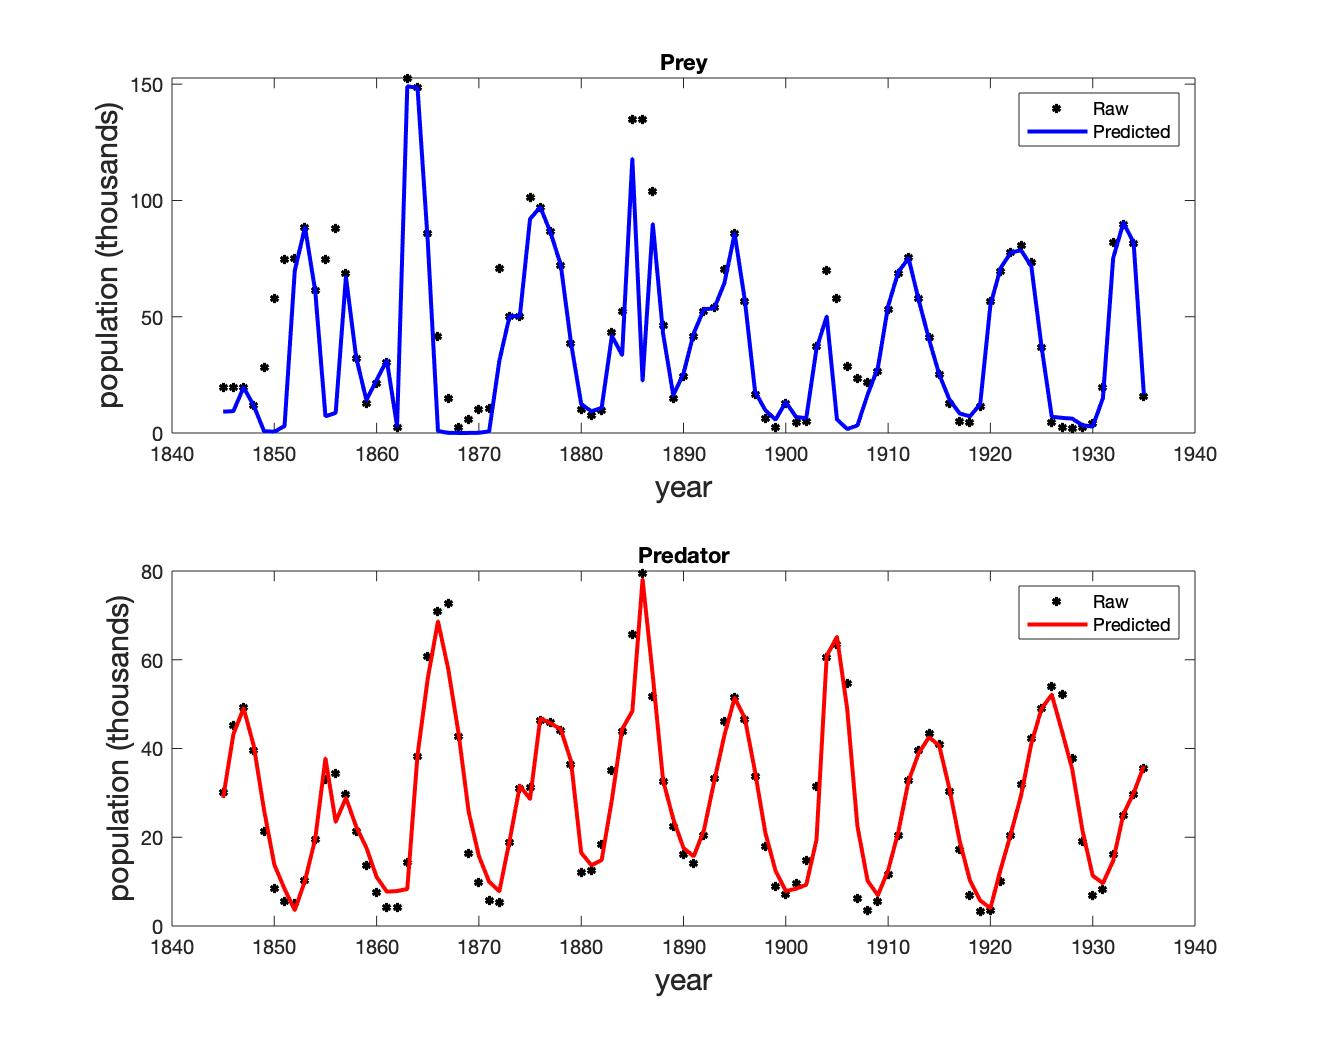
\includegraphics[width=15cm]{Kalman_Filter_Images/LV_Joint_StateEstimation.jpg}
    \caption{State estimation of Hare and Lynx data using Joint UKF. The estimates produced by each step of the filter are plotted on top of raw data. We can see that, although some of the peaks are missed especially in earlier years, the state estimation is successful.}
    \label{fig:LV_Joint_StateEstimation}
\end{figure}

As is evident visually, the Joint UKF is successful at performing state estimation. Although we do miss a few of the peaks in the dataset, the overall performance is very much satisfactory. Next, we would like to understand the amount of parameter movement occurring during the algorithm run. To do so, we plot values of the four parameters at each iteration, as well as a solid line signifying the starting point, which were determined as described in Section \ref{section:LV_initParams}.

\begin{figure}[H]
    \centering
    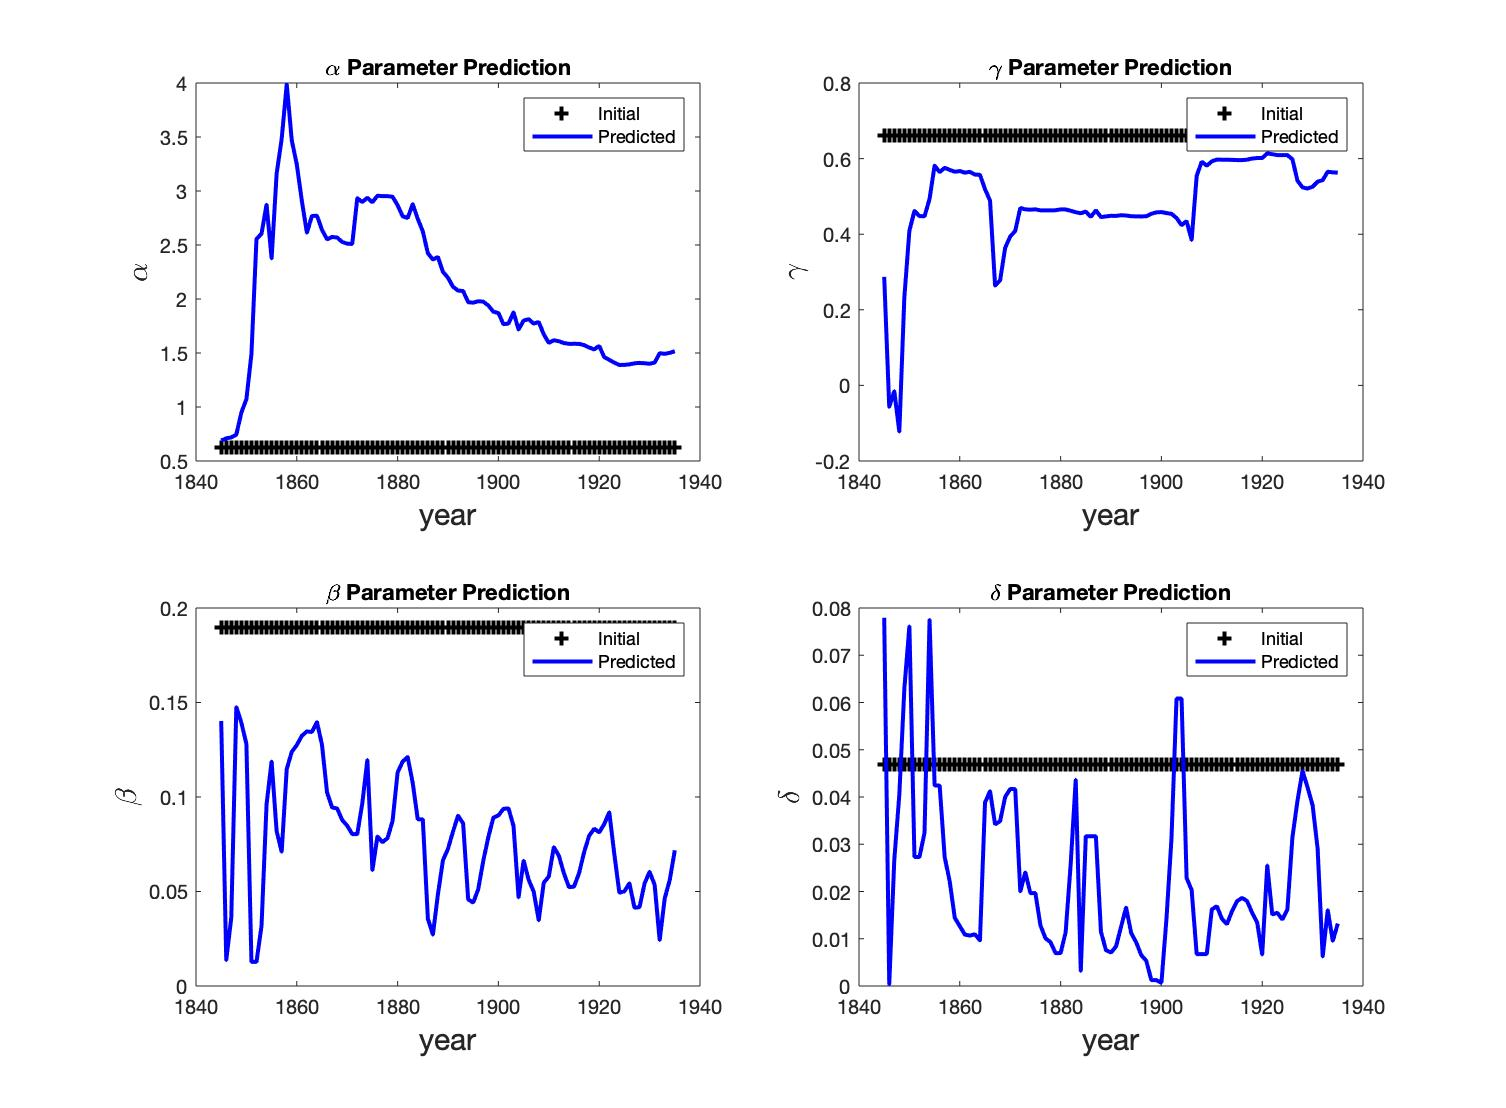
\includegraphics[width=15cm]{Kalman_Filter_Images/LV_Joint_ParamsOverTime.jpg}
    \caption{Movement of Lotka-Volterra parameters as more iterations of Joint UKF are performed. Parameters $\beta$ and $\delta$ show oscillatory behavior while $\alpha$ and $\gamma$ show better convergence towards the end of the run.}
    \label{fig:LV_Joint_ParamMovement}
\end{figure}


It is evident that there are varying amounts of parameter movement, which is dependent on the quality of the starting guess. Additionally, parameters $\beta$ and $\delta$ appear to follow an oscillatory behavior. This is likely due to the underlying time dependence in these parameters. As discussed in \textbf{Model Setup}, the parameters are assumed to be constant values. However, since the size of the peaks, troughs, and time between them is not consistent in this dataset, it is likely that the parameters are not in fact consistent, due to outside factors not included in this model. Thus, is it is likely that these parameters are oscillating in response to this phenomenon.\\
\\

Moreover, we can see, particularly for $\alpha$ and $\gamma$, that the parameters are beginning to converge towards the latter portion of the runtime. The final assessment of the algorithm's success is to understand the quality of the final parameter estimates, which will be done in section \ref{section:DualUKF}.


\subsubsection{Dual UKF} \label{section:DualUKF}
We now consider the manner in which the Dual UKF was implemented for the Predator Prey model. Since the Dual UKF runs two filters simultaneously, we must set up two different state space models, one for the states and one for the parameters. For the states, we have:
\begin{equation}
x_k = \begin{bmatrix}
h\\
l\\
\end{bmatrix} = \begin{bmatrix}
f_h(h,l)\\
f_l(h,l)\\
\end{bmatrix} + \begin{bmatrix}
q_h\\
q_l\\
\end{bmatrix}
\end{equation}
\begin{equation}
y_k = \begin{bmatrix}
y_1\\
y_2\\
\end{bmatrix} = 
\begin{bmatrix}
1 & 0\\
0 & 1\\
\end{bmatrix}
\begin{bmatrix}
h\\
l\\
\end{bmatrix}+
\begin{bmatrix}
r_1\\
r_2\\
\end{bmatrix}
\end{equation}

As in the Joint, $f_h$ and $f_l$ are the solutions to the Lotka-Volterra ODE model, which will be approximated in our code, $q_h$ and $q_l$ represent the added process noise, $r_1$ and $r_2$ represent the added measurement noise, and $y_1$ and $y_2$ represent the two observables, which in this case are the same as our states $h$ and $l$.\\
The state space model for the parameters is
\begin{equation}
x_k = \begin{bmatrix}
\alpha\\
\gamma\\
\beta\\
\delta
\end{bmatrix} = \begin{bmatrix}
\alpha\\
\gamma\\
\beta\\
\delta\\
\end{bmatrix} + \begin{bmatrix}
q_{\alpha}\\
q_{\gamma}\\
q_{\beta}\\
q_{\delta}
\end{bmatrix}
\end{equation}
\begin{equation}
y_k = \begin{bmatrix}
y_1\\
y_2\\
\end{bmatrix} = 
\begin{bmatrix}
f_{h}'(\alpha, \gamma, \beta,\delta)\\
f_{l}'(\alpha, \gamma, \beta,\delta)
\end{bmatrix}+
\begin{bmatrix}
r_1\\
r_2\\
\end{bmatrix}
\end{equation}
We define $f_h'$ to be some function of $\alpha, \gamma, \beta$ and $\delta$ such that $f_h' = h$ and $f_l'$ to be  some function of $\alpha, \gamma, \beta$ and $\delta$ such that $f_l' = l$. Notice that there is not a transition function for the parameters, since they are assumed to be constant. \\

As stated before, we should have that $R_{param} = R_x$ \cite{GoveHollingerDual}. Thus, both were set to the matrix
\begin{equation}
R = \begin{bmatrix}
30 & 0\\0 & 15\end{bmatrix} 
\end{equation}
as was done for the Joint UKF.

\paragraph{Process Covariances}
The Predator-Prey model presents the special scenario where the populations, which are our states here, are known beforehand. Thus, process noise can be determined analytically. Using the model ODEs, we produce vectors of predator and prey populations as simulated by these equations. Then, we calculate the covariance of the differences between the populations and the raw data in order to estimate the covariance of the process noise. Having these values helped us understand the \emph{ratios} between different elements in the matrix $Q_x$. However, we found that we could not use the values as is because they were too large and thus needed to scale them accordingly. In the end, we utilized:
\begin{equation}
Q_{x} = 180 * \begin{bmatrix} 1.3444 & 0.1594\\ 0.1594 & 0.4845\end{bmatrix}
\end{equation}

This approach, however, cannot be applied to the Joint, due to the issues of high process noise being assigned to populations as discussed earlier. Next, we stay consistent with \cite{GoveHollingerDual} in using
\begin{equation}
 Q_{param} = .01 * P_{param_0} 
\end{equation}


\paragraph{Initial State and Parameter Covariances}
Beginning with $P_{x_0}$, we found that
\begin{equation}
P_{x_0} = \begin{bmatrix}
20 & 0\\0 & 15\end{bmatrix}
\end{equation}
produced the best results. It is simple to see here that these are simply the first two diagonal entries from the Joint UKF's $P_0$. \\
\\
Next, we must define $P_{params_0}$. In the predator prey model, variances for $\alpha, \beta, \gamma$ and $\delta$ were assigned as 0.5, 0.7, 0.02, and 0.02 respectively. Note here that these are the same as the Joint UKF variances, apart from the increase in $\beta$'s value. This means that the diagonal of the matrix consisted of these 4 values. The off diagonal was set to .001 in order to allow for slight covariance between parameters. Putting this together, we get the matrix
\begin{equation}
P_{params_0} = \begin{bmatrix} 0.5 & 0.001 & 0.001 & 0.001 \\
                                0.001 & 0.7 & 0.001 & 0.001 \\
                                0.001 & 0.001 & 0.02 & 0.001 \\
                                0.001 & 0.001 & 0.001 & 0.02 \end{bmatrix}
\end{equation}
                                
                                

\paragraph{Dual UKF Results}
The process of assessing the quality of the Dual UKF algorithm is identical to those outlined in the \textbf{Joint UKF Results} section. Thus, first looking at the state estimation and RMSE values in figure \ref{fig:LV_Dual_StateEstimation} we have:

\begin{figure}[H]
    \centering
    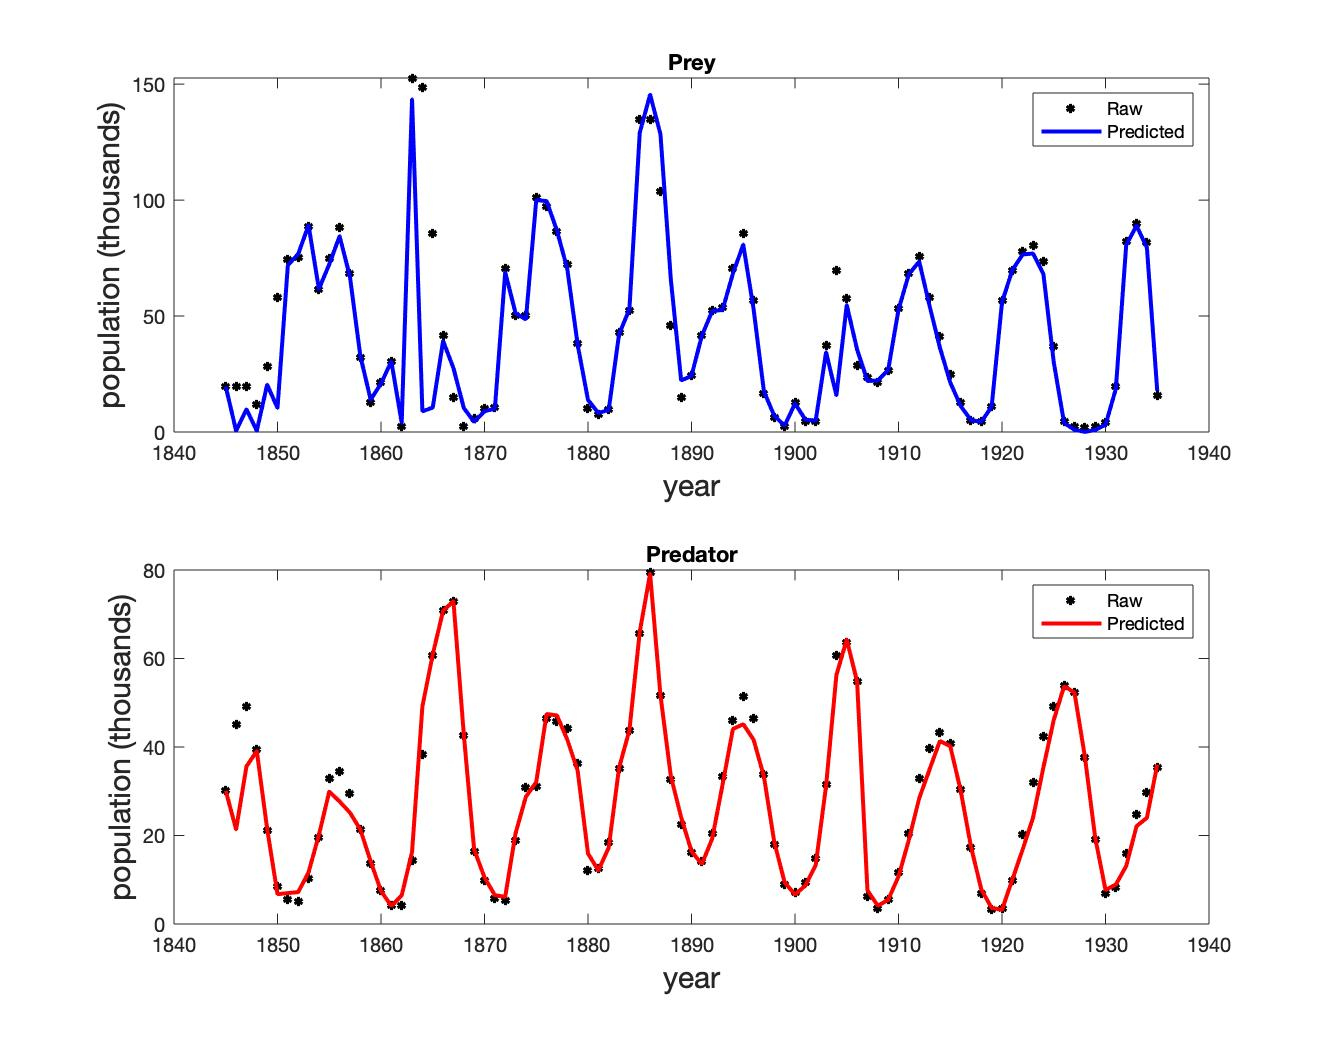
\includegraphics[width=15cm]{Kalman_Filter_Images/LV_Dual_StateEstimation.jpg}
    \caption{State estimation of Hare and Lynx data using Dual UKF. The estimates produced by each step of the filter are plotted on top of raw data. These results are very similar to the Joint UKF, where we do not meet all of the peaks in the early behavior but overall have satisfactory performance, especially for the latter end of the dataset.}
    \label{fig:LV_Dual_StateEstimation}
\end{figure}



Once again, visually speaking the Dual UKF is successful at performing state estimation. Since it is difficult to distinguish between the quality of the state estimation between the Joint and Dual approaches visually, we then consider the differences in RMSE's in Table \ref{table:LV_StateEstimation_RMSE}. Note once again that we use only Final 50\% RMSE so as to allow the algorithm to learn before judgment. It is evident that the Dual outperforms the Joint in state estimation for both the Prey and Predator populations. However, it is important to note that this is only one of our metrics for assessing performance.

\begin{table}[H]
  \begin{center}

    \begin{tabular}{c|c|c} % <-- Alignments: 1st column left, 2nd middle and 3rd right, with vertical lines in between
      \textbf{Population} & \textbf{Joint} & \textbf{Dual} \\
      \hline
      \textbf{Prey} & 9.7514 & 8.2970\\
      \textbf{Predator} & 3.8969 & 2.6533
    \end{tabular}
    \caption{Final 50\% Root Mean Squared Error (RMSE) for state estimation of Lotka-Volterra system separated by Joint and Dual UKF's. It is clear analytically that the Dual UKF performs better at state estimation.}
    \label{table:LV_StateEstimation_RMSE}
  \end{center}
\end{table}

To assess parameter values, we once again plot the movement of their values over time:
\begin{figure}[H]
    \centering
    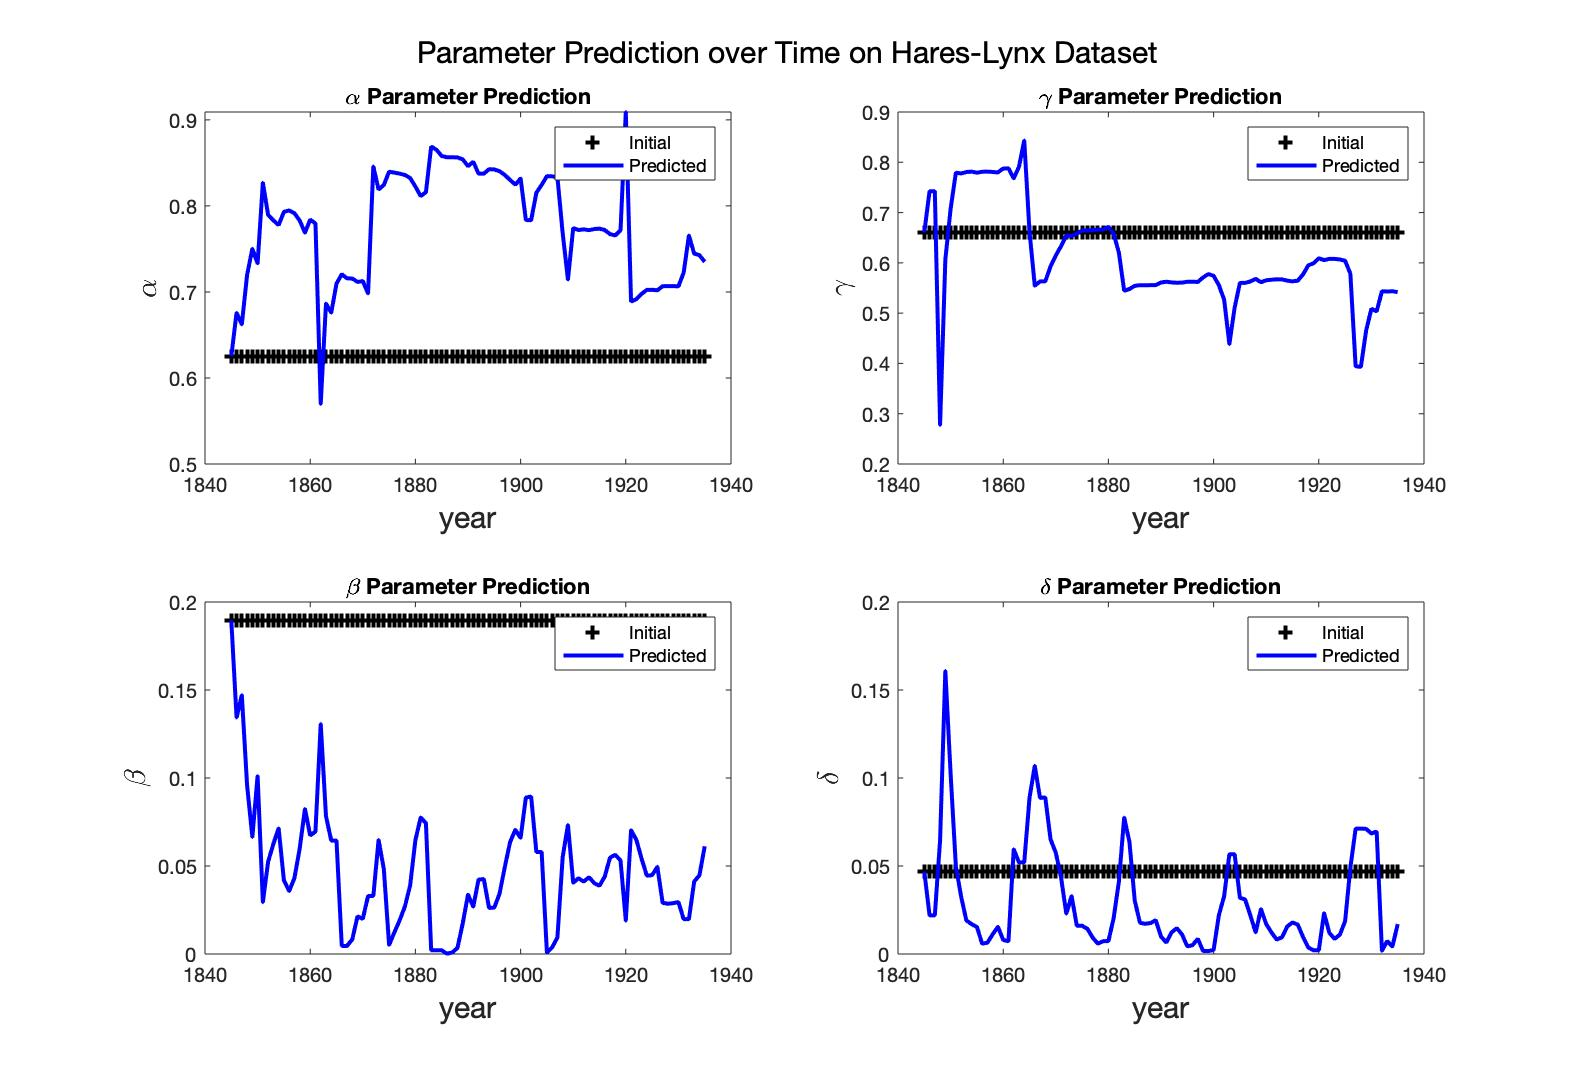
\includegraphics[width=15cm]{Kalman_Filter_Images/LV_Dual_ParamsOverTime.jpg}
    \caption{Movement of Lotka-Volterra parameters as more iterations of the Dual UKF are completed.}
    \label{fig:LV_Dual_ParamMovement}
\end{figure}

As with the Joint, there is a range of how much the parameters are moving. It is likely that the values are oscillating due to outside factors not in the model. It is important to note that the final parameter values from the joint and dual produce different results, as summarized in Table \ref{table:LV_ParamValues}.
\begin{table}[H]
  \begin{center}
    \label{tab:table2}
    \begin{tabular}{c|c|c|c} % <-- Alignments: 1st column left, 2nd middle and 3rd right, with vertical lines in between
      \textbf{Parameter} & \textbf{Initial} & \textbf{Joint} & \textbf{Dual} \\
      \hline
      \textbf{$\alpha$} & 0.623 & 1.5164 & 0.7349\\
      \textbf{$\beta$} & 0.1896 & 0.0718 & 0.0612\\
      \textbf{$\gamma$} & 0.6607 & 0.5629 & 0.5417\\
      \textbf{$\delta$} & 0.0468 & 0.0132 & 0.017
    \end{tabular}
    \caption{Initial parameter values as well as final parameter estimates from the Joint and Dual UKF's. It is evident that overall the Joint UKF results in more parameter movement than the Dual}
    \label{table:LV_ParamValues}
  \end{center}
\end{table}
The final assessment of the dual is to consider the quality of the ODE as simulated with the final parameter values, which will be performed for both forms of the UKF. Figure \ref{fig:LV_Joint_ODESims} displays these results for the Joint UKF, and Figure \ref{fig:LV_Dual_ODESims} for the Dual. 

\begin{figure}[H]
    \centering
    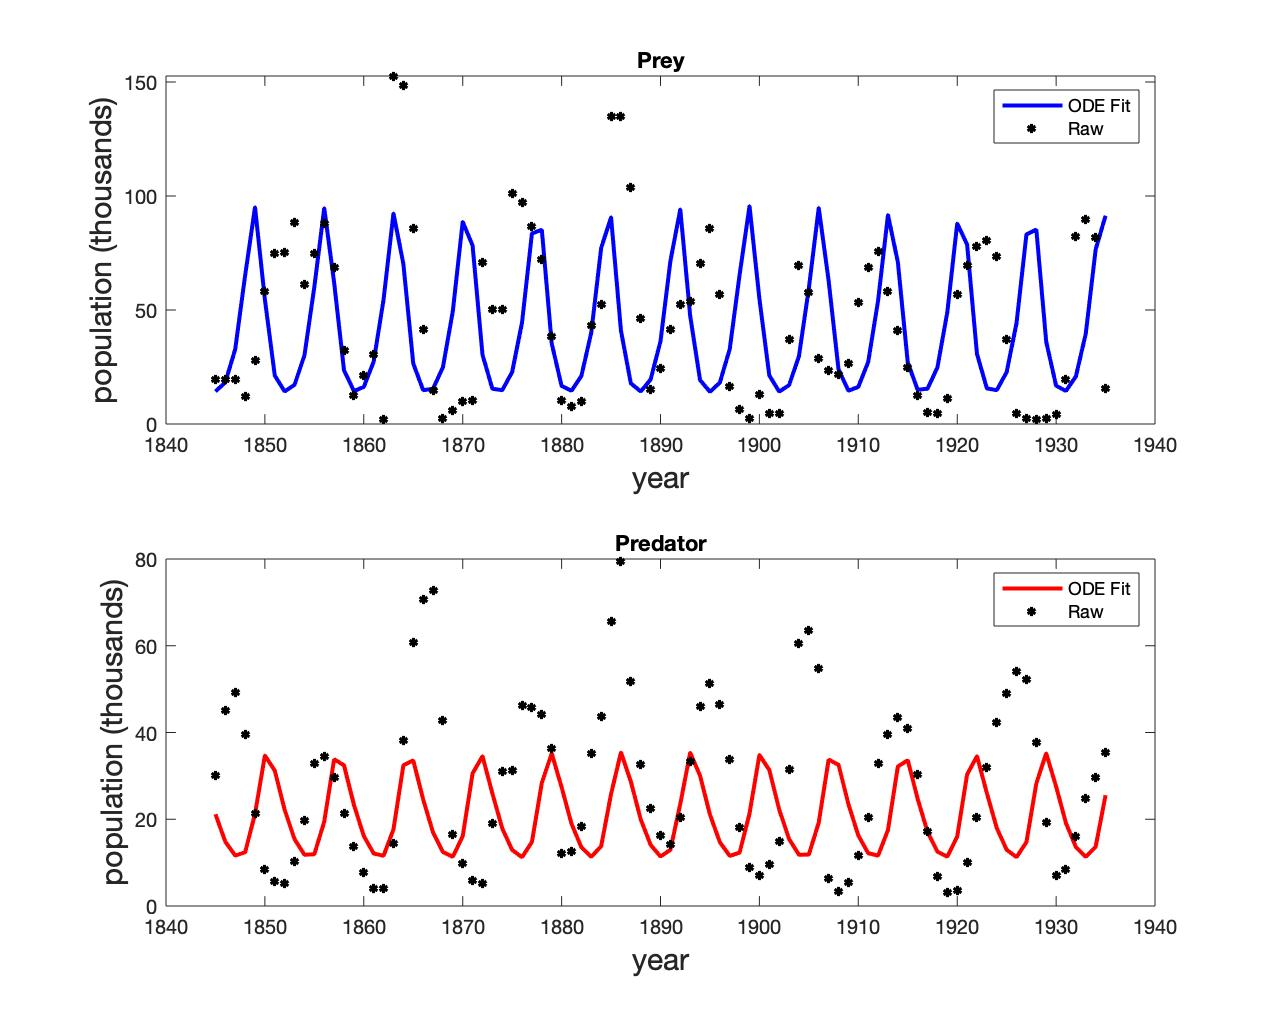
\includegraphics[width=15cm]{Kalman_Filter_Images/LV_Joint_ODEFits.jpg}
    \caption{Plot of system simulated with final parameters outputted from Joint UKF over top of raw data. The main issue with this fit is that the frequency of the final ODE is higher then we would expect. The Dual UKF fit shown in Figure \ref{fig:LV_Dual_ODESims} performs better in this regard.}
    \label{fig:LV_Joint_ODESims}
\end{figure}

\begin{figure}[H]
    \centering
    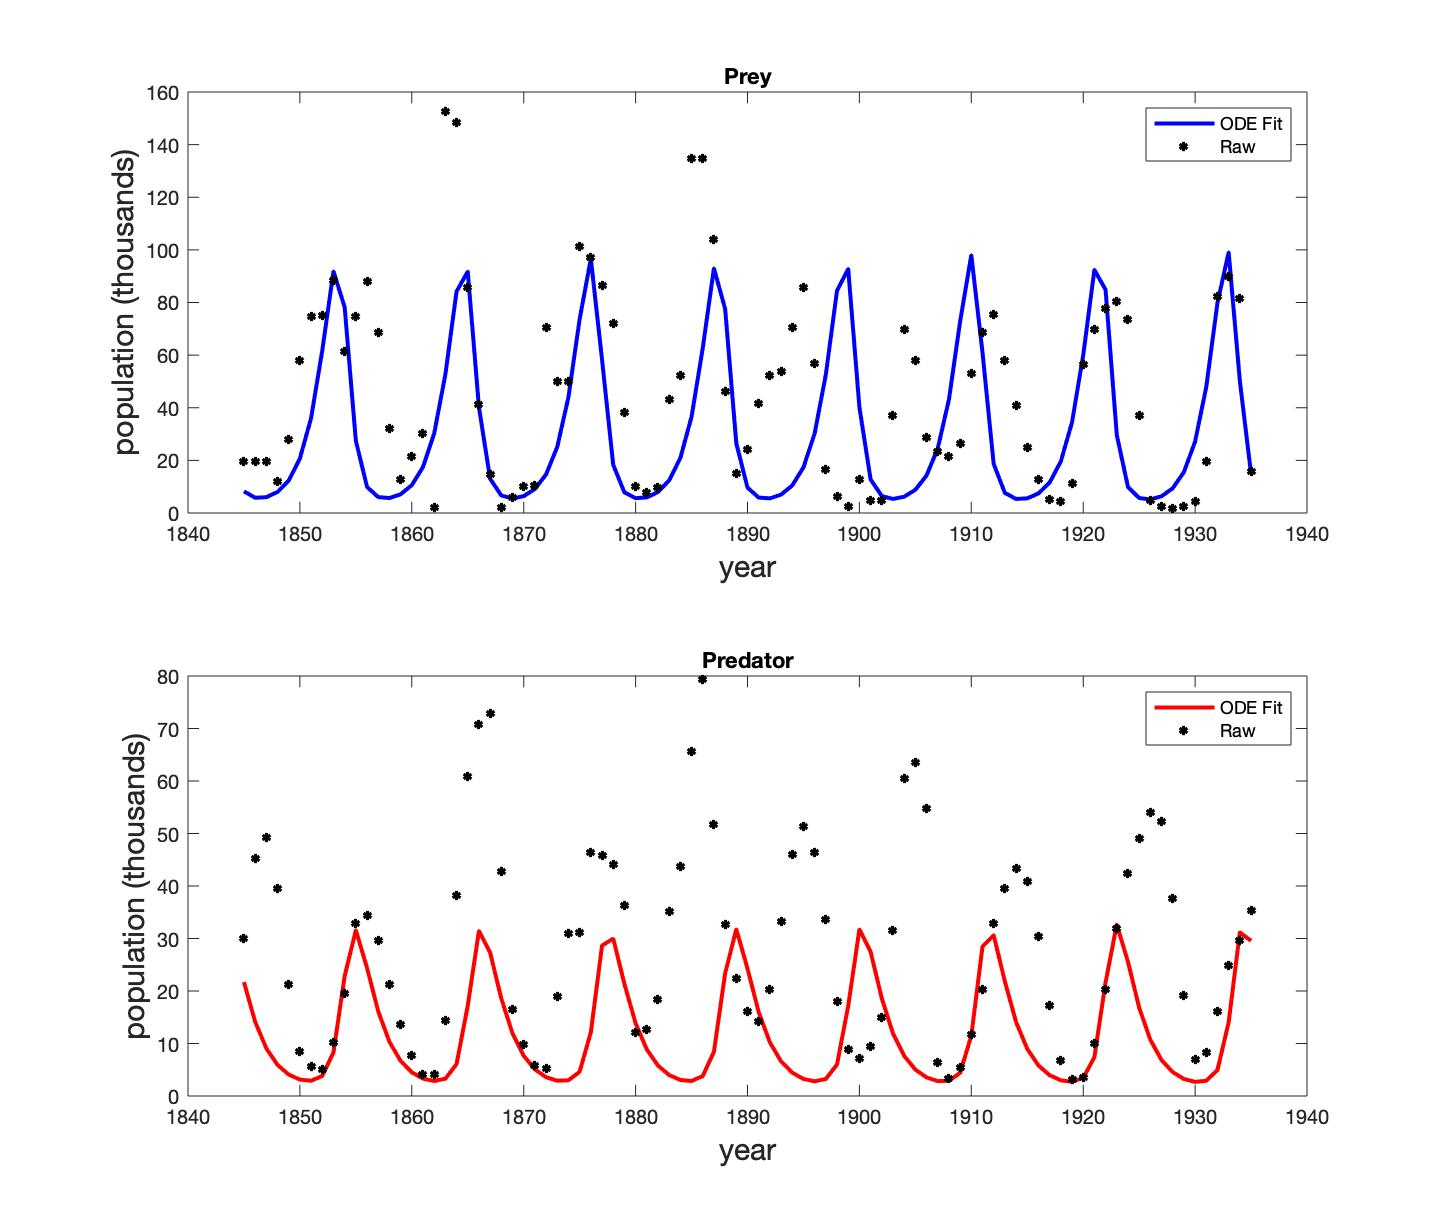
\includegraphics[width=15cm]{Kalman_Filter_Images/Lv_Dual_ODEFits.jpg}
    \caption{Plot of system simulated with final parameters outputted from Dual UKF over top of raw data}
    \label{fig:LV_Dual_ODESims}
\end{figure}

Visually, it is evident that the parameters produced from the Joint predict many more iterations of the peak-trough behavior than the Dual. This gives the initial edge to the Dual, however we need to quantify the performance to gain a better understanding of which aporach is performing better. This can be done by calculating the RMSE for the ODE's predictions. It is important to note here that, unlike for state estimation, we use RMSE for the full time frame not only the final 50\%.

\begin{table}[H]
  \begin{center}
    \begin{tabular}{c|c|c} % <-- Alignments: 1st column left, 2nd middle and 3rd right, with vertical lines in between
      \textbf{Population} & \textbf{Joint} & \textbf{Dual} \\
      \hline
      \textbf{Prey} & 42.5392 & 36.665\\
      \textbf{Predator} & 22.2058 & 25.2749
    \end{tabular}
    \caption{Root Mean Squared Error (RMSE) of ODE simulations using final parameter values from Joint and Dual UKF's from Prey and Predator populations.}
    \label{table:LV_ODESims_RMSE}
  \end{center}
\end{table}

Based on Table \ref{table:LV_ODESims_RMSE}, we see that the Dual vastly outperforms the Joint in they Prey RMSE while, on the other hand, the Joint does slightly better on the Predator populations. However, overall the Dual produces better results numerically. Similarly, the frequency of peaks produced by the Dual produced parameters as seen in Figure \ref{fig:LV_Dual_ODESims} more closely fit our biological intuition about the system than the Joint parameters. Thus, we will say that \emph{the Dual UKF produces the best UKF fit to the Predator-Prey system}.


\paragraph{A Note on Choosing an Algorithm}
In the context of the Predator-Prey model we have been successful at using both the Joint and Dual UKFs. However, in this context we have the luxury of a relatively simple system. When systems become more complex, though, a decision must be made on which approach to use. Each algorithm provides one main advantage: The Joint UKF allows for covariance between states and parameters, and the Dual UKF separates out noise between the states and parameters \cite{GoveHollingerDual}. As a general guideline, when a system is very complicated and data noisy, the Dual UKF will likely provide better results. However, it may often be useful to implement both approaches and then compare results and choose one to move forward with.
\\

\subsection{Kalman Filter Implementation on T1D Model} \label{section:UKF_T1D_Implementation}
Moving on from the Predator-Prey system, we now consider the T1D model developed by Shtylla et al. in \cite{shtylla2019mathematical}. Once again, both the Joint and Dual UKF's were implemented and compared. Since we implemented T1D after Predator-Prey, we can now also build on what we have learned about UKF's from Predator-Prey when approaching this new system.

\subsubsection{Model Set Up}
Analogously to our Predator-Prey system, we once again must establish our states and parameters. Here, states are all the various pancreas cell counts included in the model. Importantly, the one state which we can observe, and is thus our \emph{observable} in this context is Glucose. \\
\\
41 parameter values were estimated, a full list of which can be found in the \textbf{Appendix}. While there are too many states and parameters to show the full state space model, the set up is analogous to the predator-prey which can be viewed in equations 7-10 (Joint), and 13-16 (Dual). A key parameter which was not estimated is the Macrophage Clearance Rates, a parameter currently too sensitive to estimate as slight deviations, without proper compensation in other parameters, can result in undefined behavior. However, Macrophage Clearance Rates will be crucial to incorporate into the set of estimated parameters moving forward.

\paragraph{Importance of Estimating All Parameters}
Our initial intuition was that, due to computational constraints, it would be best to only estimate a subset of the model parameters, those which we deemed to be most sensitive using eFAST. However, following this approach produced very inaccurate results. This is due to the underlying relationships between parameters through the system of ODE's. By pinning down most parameters and only allowing some to move, we obtained biologically implausible parameter combinations. Thus, it is necessary to allow all parameters to move at least slightly. This "wiggle room" greatly improved performance and is now seen as a prerequisite for the UKF algorithms to work as expected.


\subsubsection{Determining Success of Algorithm}
Before entering specifics of the Joint and Dual UKF's and their results, it is important to establish what metrics will be used to determine success here. The first main metric will be RMSE of the Glucose function plotted with final parameter values against the raw data. When transitioning to T1D, the quality of the Glucose state estimation, although considered, has taken a back seat to this RMSE calculation. Second, we are interested in the biological feasibility of our results. The set of final parameters our algorithms output determine not only the behavior of Glucose but of the other 11 cell counts as well. Thus, the possibility exists for our Glucose fits to be excellent while the behavior of the other cells is biologically impossible. Thus, we will plot other states of our model using the final parameters and visually assess behavior. \\
\\
Our last check is once again a biological one. The parameter values of the ODE model are meant to ``live on the edge". By this, we mean that the NOD mouse should get sick if it experiences an apoptotic wave and remain healthy otherwise \cite{shtylla2019mathematical}. Thus, we plot the system with and without the wave in order to check whether this is the case. Both of these biological checks are performed in Section \ref{Results_Biological_Feasibility}. Having established our criteria for success, we can now continue to the setup of the UKF's.


\subsubsection{Code Structure}
In previous work, Kalman Filters have been exclusively run on a dataset a single time, and this process is most similar to the context in which Kalman Filters have been used historically, such as for predicting rocket trajectories. However, with both Lotka-Volterra and T1D, we have the benefit of looking at the data retrospectively, meaning that all of the data is available before we begin. As a result, we have the experiment with training the model on the same data set multiple times. The potential benefit of this approach is that the Kalman Filter has more opportunities to make corrections to parameters when more data points are present. Thus, we suspect that this can improve the final fit. The process for doing this is as follows:
\begin{enumerate}
    \item Initialize a parameter guess $param_0$.
    \item Run the UKF.
    \item Set $param_0$ equal to final output of UKF .
    \item Repeat steps 2 and 3 as many times as desired.
\end{enumerate}
Although it had little effect on results in the context of Lotka-Volterra, this proved to be very effective for T1D. For example, what we found is that the number of runs needed to reach the optimal fits in Figure \ref{fig:T1D_Dual_AllAcute_Plots} varied by mouse. As seen in the code workflow in Figure \ref{fig:T1D_CodeFlow}, after 5 iterations we choose the best result, as determined by RMSE, to call our "best fit". Future work to standardize the number of iterations needed or possibly reduce the number of iterations to 1 is recommended and discussed in section \ref{section:UKF_FutureImprovements}.
\begin{figure}[H]
    \centering
    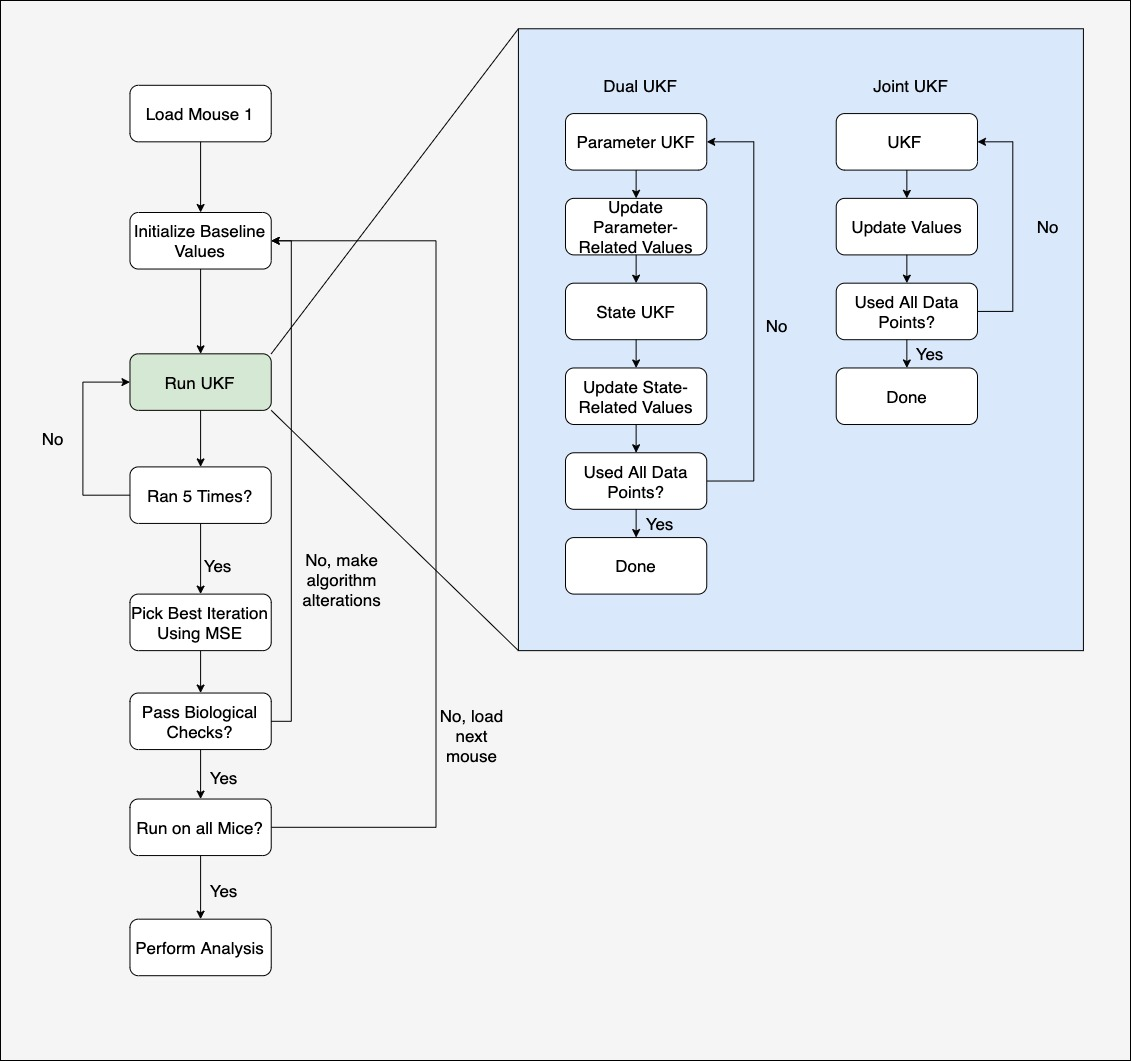
\includegraphics[width=17cm]{Kalman_Filter_Images/Workflow_FlowChart.jpg}
    \caption{Flow chart depicting the structure of code used to fit parameters to T1D model. Notice that multiple iterations are performed in order to determine the best fit.}
    \label{fig:T1D_CodeFlow}
\end{figure}
In addition to the role of multiple iterations, we can also see here that the general structure of the code is independent of whether a Dual or Joint UKF is being used. Additionally, it demonstrates that Biological Checks as described in section \ref{Results_Biological_Feasibility} must be completed before determining that an iteration on a specific mouse has been successful. Lastly, it is important to note that there are occurrences where, for example, the results after iteration 3 are worse than those from iteration 2. This is a surprising result and is why we choose the \emph{best} run of 5 iterations instead of consistently choosing the fifth. This discrepancy is likely due to the manner in which parameter variances are set in the algorithm. Towards later iterations the variances are now too high and we should not be searching as much of parameter space as we are. Thus, looking more into how to reduce variances as more and more iterations are completed is recommended and discussed in section \ref{section:UKF_FutureImprovements}.\\
\\
Let us now begin the discussion of the specifics regarding the algorithm set up.




\subsubsection{Common Parameters}
Once again we begin by considering the values of $\alpha$, $\kappa$, $\beta$, and the measurement noise $R$, values common to the Dual and Joint approaches. $\alpha$ is once again set to a small value, this time 10e-4. Values of $\kappa$ and $\beta$ were kept constant when transitioning to the T1D model from Predator-Prey, meaning that they are 0 and 2 respectively. However, we have a drastic shift in our approach to approximating $R$.\\
\\
Using baseline parameter values from A. Do, we can simulate Glucose values over time. Using this, we can then compare to our measured Glucose values and take the variance of differences at each time point in order to construct $R$. Since we only have a single observable, here $R$ will be a single variance value. Additionally, $R$ can be calculated on a mouse-by-mouse level, helping the algorithm work across a wide range of mice data sets.

\subsubsection{Dual UKF}
The state space model for the Dual UKF for the T1D model is set up in an analogous way to the predator-prey model. The state space model for the states is set up as a vector of the states represented by the solved version of their respective ODE's  with some process noise added on. The observable equation, which is just glucose, contains a matrix which filters out only glucose from the states, with a little measurement noise added in. \\
\\
The state space model for the parameters is also set up similarly. The state equation for the parameters is a simple identity transformation with a bit of process noise added in. And the observable equation is some function of the parameters that is equal to the value of glucose, with a little bit of measurement noise added in. 

\paragraph{Process Covariances}\label{section:T1D_Dual_ProcessCovariance}
Let's begin with $Q_x$. In the T1D model, since there is no knowledge of the states apart from Glucose, noise needs to be estimated in an ad hoc fashion. To do this, the feasible range of the state was considered in order to estimate a noise value that was on a similar scale of magnitude to those values. Then, they were tuned in order to better the system's fits. In the end, a diagonal matrix was used where each state had an assigned noise covariance. For the sake of readability, Table \ref{table:T1D_Dual_StateNoiseVariances} provides each noise variance for a given state. These values are then placed along the diagonal to create $Q_x$.

\begin{table}[H]
  \begin{center}

    \begin{tabular}{c|c} % <-- Alignments: 1st column left, 2nd middle and 3rd right, with vertical lines in between
      \textbf{State} & \textbf{Noise Variance} \\
      \hline
      \textbf{Resting Macrophage} & 1000\\
      \textbf{Activated Macrophage} & 1000\\
      \textbf{Apoptotic Beta} & 1000\\
      \textbf{Necrotic Beta} & 700\\
      \textbf{Healthy Beta} & 100\\
      \textbf{Glucose} & 50\\
      \textbf{Insulin} & 2\\
      \textbf{Immunogenic DC} & 100\\
      \textbf{Tolerogenic DC} & 1000\\
      \textbf{Effector T} & 10000\\
      \textbf{Regulatory T} & 100\\
      \textbf{Memory T} & 200
    \end{tabular}
    \caption{Noise variance values for each state in the T1D system. These variances are placed along the diagonal of $Q_x$ with zeros everywhere else. Values were determined ad hoc and are on the same order of magnitude as the state values themselves.}
    \label{table:T1D_Dual_StateNoiseVariances}
  \end{center}
\end{table}

Next, we follow the same literature used to set $Q_param$ for the Predator-Prey model, meaning that we have
\begin{equation}
Q_{param} = .01 * P_{param_0}
\end{equation}
here as well.

\paragraph{Initial State and Parameter Covariances}\label{section:T1D_Dual_InitialCovariances}
Beginning with $P_{x_0}$, we were able to initialize to a square matrix of all ones in the case of T1D. If you recall from Predator-Prey, there covariances between states were left as 0, however here due to the complexity of the interactions between cells in the pancreas it is best to make those non-zero. $P_{params_0}$, as in the Predator-Prey system, proved to be crucial. Once again, due to readability we provide Table \ref{table:T1D_Dual_ParamVariances} with the variance assigned to each parameter.


\begin{table}[H]
  \begin{center}
    \begin{tabular}{c|c} % <-- Alignments: 1st column left, 2nd middle and 3rd right, with vertical lines in between
      \textbf{Parameter} & \textbf{Variance} \\
      \hline
      J & 200\\
      k & 0.05\\
      {b} & 0.005\\
      {c} & 0.05\\
      {$e_1$} & 10e-10\\
      {$e_2$} & 10e-10\\
      {fD} &10e-12\\
      {ftD} & 10e-12\\
      {$\alpha_B$} & 10e-4\\
      {$\delta_B$} & 10e-3\\
      {$B_{conv}$} & 10\\
      {Ghb} & 2\\
      {$R_0$} & 2\\
      {$EG_0$} & 0.02\\
      {SI} & 5\\
      {$\sigma_I$} & 5\\
      {$\delta_I$} & 10\\
      {GI} & 175\\
      {$Q_{panc}$} & $10^-3$\\
      {$Q_{blood}$} & $10^-3$\\
      {$Q_{spleen}$} & $10^-3$\\
      {$\mu_{PB}$} & $10^-3$\\
      {$\mu_{BP}$} & $10^-3$\\
      {$D_{ss}$} & 175\\
      {bDEday} & $10^-11$\\
      {bIRday} & $10^-11$\\
      {aEaday} & $10^-4$\\
      {$T_{naive}$} & 1\\
      {bpday} & 4\\
      {ramday} & $10^-3$\\
      {baEday} & $10^-5$\\
      {baRday} & $10^-5$\\
      {aEmday} & $10^-5$\\
      {$\mu$} & $10^-3$\\
      {thetaD} & 200\\
      {d} & 1\\
      {sE} & 1\\
      {sR} & 1\\
      {$\alpha_\eta$} & 5\\
      {$\beta_\eta$} & 15\\
      {$\eta$} & .0001
    \end{tabular}
    \caption{Variance values for each parameter being estimated in the T1D model. These values are placed along the diagonal, with zeros everywhere else, to create $P_{params_0}$. These values have been found to be very important and should be tuned individually.}
    \label{table:T1D_Dual_ParamVariances}
  \end{center}
\end{table}

In the T1D model, the importance of parameters ranges tremendously. By this we mean that a small shift in some parameters can drastically change the outcome of the system while others are less crucial. Thus, this \emph{sensitivity} is important to consider when determining variance values. Additionally, through experimentation, parameters were determined that tended to move from their baseline values more than others. Thus, these values must be assigned larger variances in order to allow for the movement necessary to fit the given data. Specifically, examples of such parameters are found in Tables \ref{table:T1D_Dual_ParamChange} and \ref{table:T1D_Joint_ParamChange}.\\
\\
Thus, these variances have been determined through experimentation specifically with the Li dataset. In the event that new datasets are incorporated, one will need to consider these variances depending on how similar the data is to the baseline parameter values. Additionally, following new sensitivity analysis results these values will need to be reconsidered as well. 



\paragraph{Dual UKF Results} \label{section:T1D_DualUKF_Results}
We are interested in assessing results on a wide range of mice, including those which are acute as well as progressive. Let's begin with the acute mice.

\subparagraph{Acute Mice}
As specified previously, acute mice make a drastic transition from the healthy to unhealthy state, categorized by a ``Z" shape in the glucose levels. When the definition is applied to the Li dataset, we are left with 9 data sets. We ran the Dual UKF on each mouse and obtained best fit RMSE values by comparing the simulated ODE using the final parameters to the raw dataset. Figure \ref{fig:T1D_Dual_AllAcute_Plots} displays the 9 fits while Table \ref{table:T1D_Dual_AllAcute_RMSE} contains the RMSE values.\\

\begin{figure}[H]
    \centering
    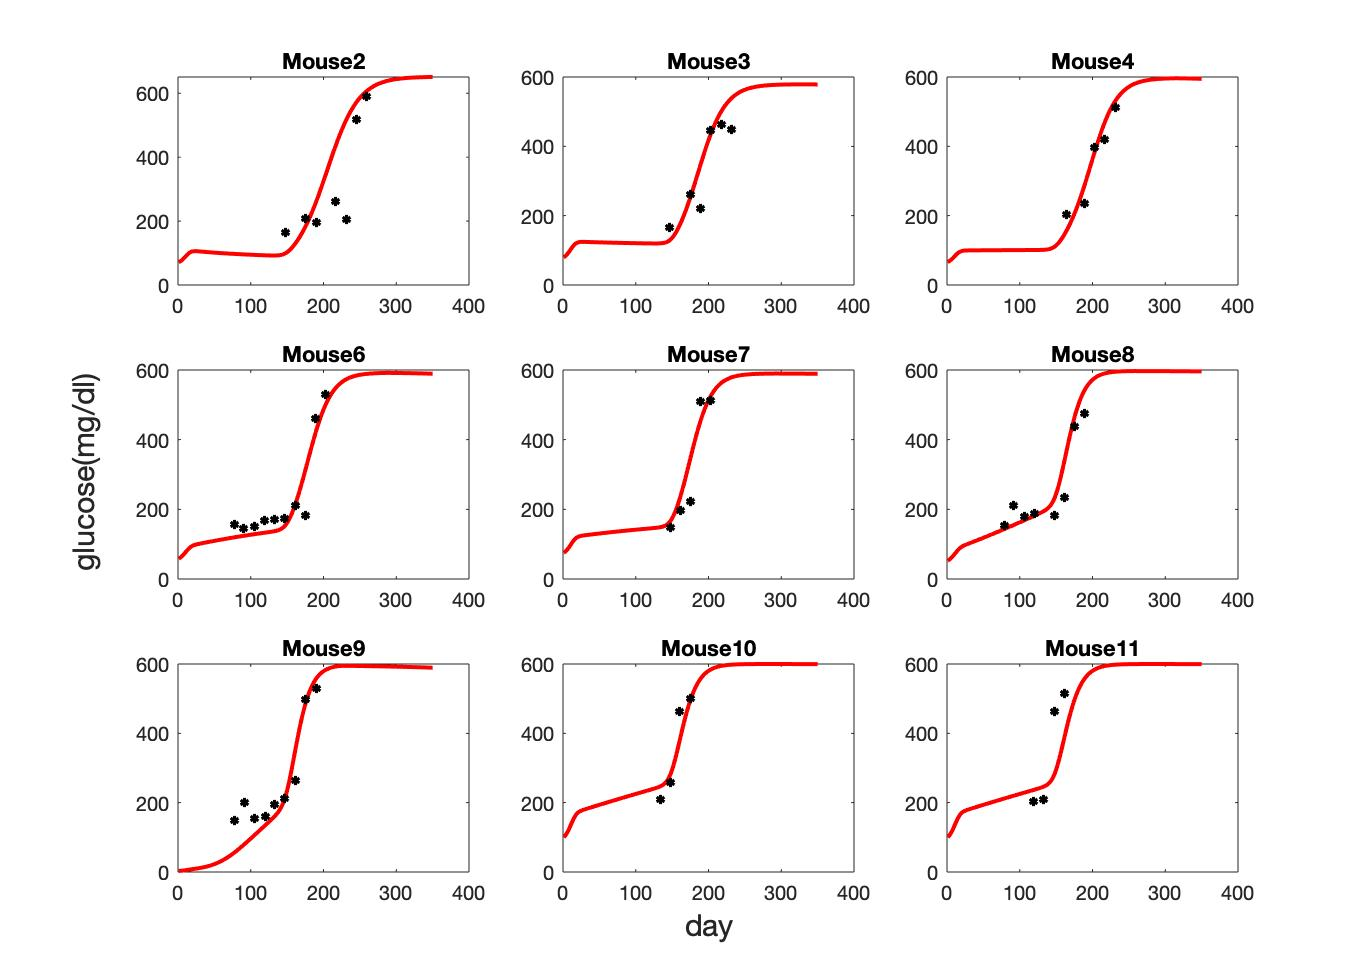
\includegraphics[width=15cm]{Kalman_Filter_Images/Dual_Acute_Mouse_Fits.jpg}
    \caption{All best fits for acute NOD mice. The ODE system using the final parameter estimates is plotted against the raw data. It is evident that the algorithm is functioning correctly, however there is room for improvement, most likely through experimentation with parameter variances.}
    \label{fig:T1D_Dual_AllAcute_Plots}
\end{figure}

\begin{table}[H]
  \begin{center}
    \begin{tabular}{c|c} % <-- Alignments: 1st column left, 2nd middle and 3rd right, with vertical lines in between
      \textbf{Mouse Number} & \textbf{RMSE} \\
      \hline
      \textbf{2} & 141.074\\
      \textbf{3} & 67.4255\\
      \textbf{4} & 40.8032\\
      \textbf{6} & 50.1488\\
      \textbf{7} & 60.4445\\
      \textbf{8} & 50.6606\\
      \textbf{9} & 62.4348\\
      \textbf{10} & 45.3828\\
      \textbf{11} & 114.4727
    \end{tabular}
    \caption{Root Mean Squared Error (RMSE) of ODE simulations using final parameter values for Acute mice from Dual UKF on T1D model. This confirms our visual understanding that errors overall are low however could likely be improved further.}
    \label{table:T1D_Dual_AllAcute_RMSE}
  \end{center}
\end{table}
It is evident that the Dual UKF is successful across a range of mice, however performance is of course dependent on the data set. Largely, this is due to how "different" that dataset is from the baseline. The baseline parameters produce the glucose values in Figure \ref{fig:T1D_BaselineGlucose}. The more similar the shape of the glucose of a mouse is to that behavior, the better fit we would expect. Thus, in this lies the importance of the initial parameter guess one uses in the algorithm.

\begin{figure}[H]
    \centering
    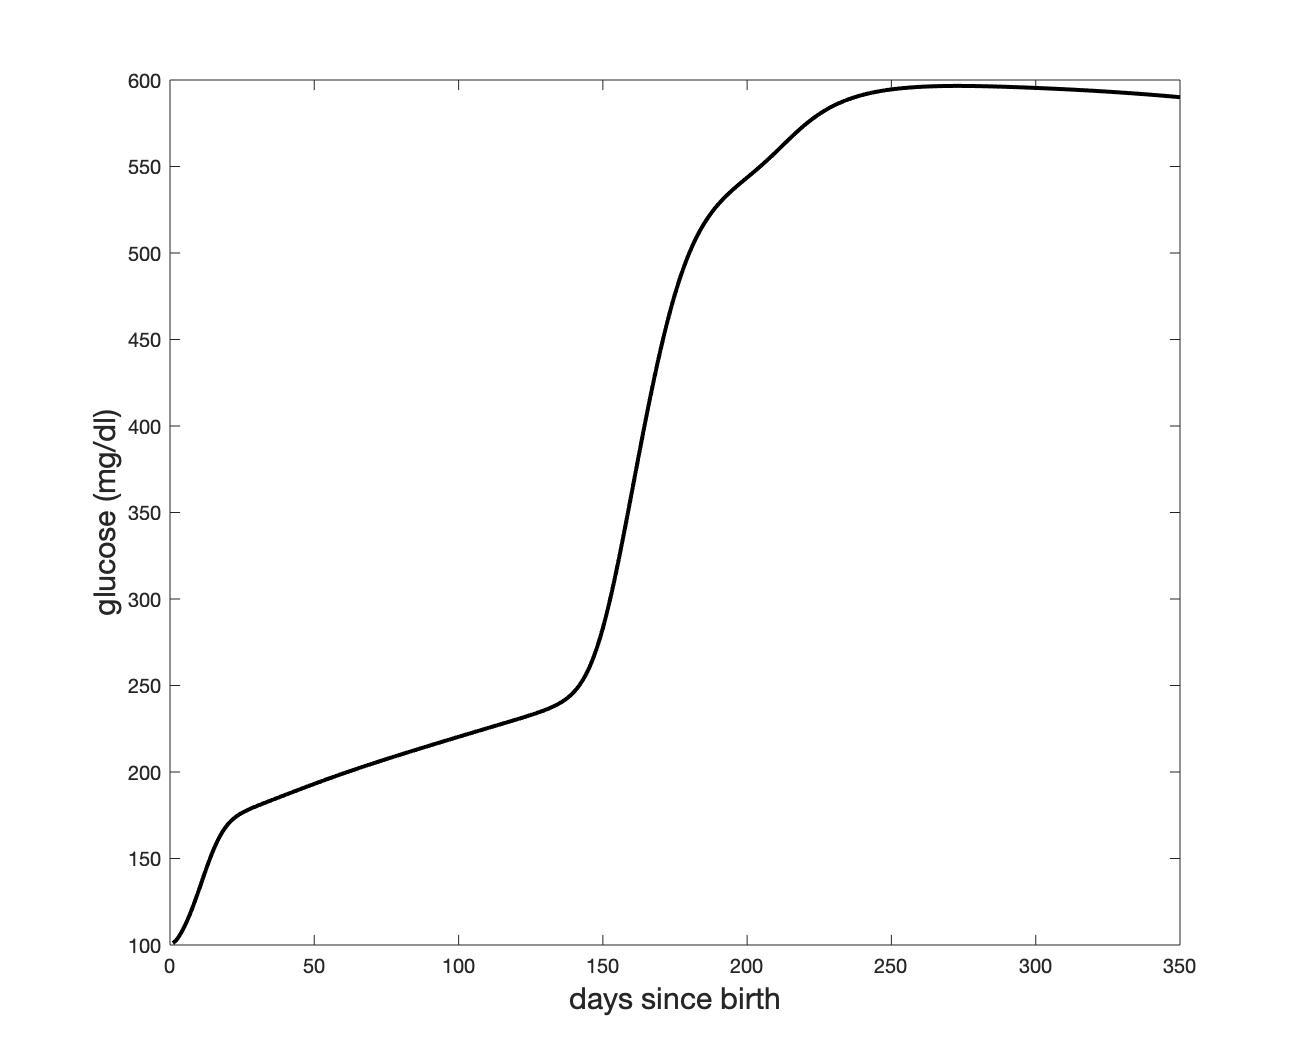
\includegraphics[width=10cm]{Kalman_Filter_Images/T1D_BaselineGlucose.jpg}
    \caption{Glucose plot for NOD mouse with wave conditions and baseline parameters. The closer a raw mouse dataset is to this behavior, the less parameter movement is required to reach an optimal fit. This motivates the importance of the initial guess and parameter variances.}
    \label{fig:T1D_BaselineGlucose}
\end{figure}



\subparagraph{Progressive Mice}
In order to examine behavior of Progressive mice, we look at mice 1 and 5. The behavior these mice is a relatively flat glucose slope towards a diabetic state. Our initial hypothesis is that the algorithm will perform poorly on these datasets due to the underlying model being geared more so towards acute behavior. Figure \ref{fig:T1D_Dual_Progressive_Plots} and Table \ref{table:T1D_Dual_Progressive_RMSE} once again display the best fit and RMSE values.

\begin{figure}[H]
    \centering
    \includegraphics[width=15cm]{Kalman_Filter_Images/Dual_Progressive_Mouse_Fits.jpg}
    \caption{Best fits for the Progressive NOD mice. It is evident that, in general, the algorithm performs worse in this scenario that in the Acute setup. This is most pronounced in Mouse 1.}
    \label{fig:T1D_Dual_Progressive_Plots}
\end{figure}

\begin{table}[H]
  \begin{center}

    \begin{tabular}{c|c} % <-- Alignments: 1st column left, 2nd middle and 3rd right, with vertical lines in between
      \textbf{Mouse Number} & \textbf{RMSE} \\
      \hline
      \textbf{1} & 86.8240\\
      \textbf{5} & 89.1078
    \end{tabular}
    \caption{Root Mean Squared Error (RMSE) of ODE simulations using final parameter values from Dual UKF run on Progressive mice for the T1D model. Once again, we see the general trend of worse fits on the Progressive, as compared to Acute, mice.}
    \label{table:T1D_Dual_Progressive_RMSE}
  \end{center}
\end{table}


As expected, the algorithm performs poorly on the progressive mouse. We can see that, in Mouse 1, the algorithm expects the sudden jump to a diabetic state that we saw in acute mice and thus is tricked by increases in glucose it expects to predict the onset. In fact, it is likely that the algorithm would need to be initiated differently, meaning different covariance matrices and initial guesses, in order to get an ideal fit for a progressive mouse. This is an aspect of the problem that we highly recommend pursuing moving forward. Additionally, we see here the importance of having both a visual and numerical check. Numerically, the mouse 1 and 5 fits are definitely comparable to the acute ones in Table \ref{table:T1D_Dual_AllAcute_RMSE}. However, visually, these fits miss both the time and slope of diabetes onset, two criteria which we value highly.

\paragraph{Analysis of Parameter Movement}
At the completion of running the Dual UKF, it is helpful to analyze how far away parameters have traveled from their original starting points, as these can be seen as the parameters having the most impact on the outputted fit. In order to gain a general understanding of the important parameters, we can look at the average deviation from the starting point and identify parameters that, on average, move greater than or equal to 1\%. The cutoff of 1\% was chosen by viewing the values for all parameters and seeing that the nearest value to 1\% was far lower.\\
\\
For a given parameter $p$ on mouse $i$, we always have $p^i_0$ and $p^i_{final}$. For example, for parameter $\mu$, $mu^2_{final}$ represents the final value of $\mu$ after the Dual UKF is run on mouse 2. Thus for every parameter $p$ and mouse $i$, we calculate:
\begin{equation} \label{eq:UKF_Param_Change}
    \Delta p^i = (p^i_{final} - p^i_0)/p^i_0 
\end{equation}
Then, for each parameter $p$ we take the average of all the $\Delta p^i$'s to get the average present change.\\
\\
For the Dual UKF, the parameters meeting the criteria of having an average change greater than 1\% are found in Table \ref{table:T1D_Dual_ParamChange}.

\begin{table}[H]
  \begin{center}
 
    \begin{tabular}{c|c} % <-- Alignments: 1st column left, 2nd middle and 3rd right, with vertical lines in between
      \textbf{Parameter} & \textbf{Average Percent Change} \\
      \hline
      \textbf{$\mu$} & 13530\%\\
      \textbf{$e_2$} & 1933\%\\
      \textbf{$e_1$} & 530.965\%\\
      \textbf{$SI$} & 483.671\%\\
      \textbf{$\delta_B$} & -32.067\%\\
      \textbf{$\alpha_B$} & 18.215\%\\
      \textbf{$GI$} & -5.642\%\\
      \textbf{$\eta$} & -3.864\%\\
      \textbf{$\sigma_I$} & 1.351\%
    \end{tabular}
    \caption{Parameters and average percent change for all those that exceed 1 percent. These parameters appear to be of utmost importance in producing the fits seen in this section.}
    \label{table:T1D_Dual_ParamChange}
  \end{center}
\end{table}

Variances for these parameters in particular were important to tune and it will be crucial to continue delving into their importance moving forward. It will also be interesting to see how these relate to parameters outputted from a formal sensitivity analysis.\\

Additionally, we are interested in seeing the spread of values for these key values. To do so, we can create box plots of the final parameter values, found in Figure \ref{fig:T1D_Dual_Parameter_BoxPlots}.

\begin{figure}[H]
    \centering
    \includegraphics[width=15cm]{Kalman_Filter_Images/Dual_Parameter_BoxPlots.jpg}
    \caption{Box plots showing distribution of parameter values for those parameters listed in Table \ref{table:T1D_Dual_ParamChange}. Outliers are marked by red plus signs. It is evident that there is a range of behaviors, with there often being outliers in the distributions.}
    \label{fig:T1D_Dual_Parameter_BoxPlots}
\end{figure}

Figure \ref{fig:T1D_Dual_Parameter_BoxPlots} demonstrates that there is a range in behavior of the parameters. For example, parameters such as $S_I$ and $G_I$ have very tight distributions apart from a few outliers, while $e_1$, $e_2$, and $\delta_B$ all have no outliers. Additionally, there is no clear pattern in the skewness of the distributions, which can be seen by comparing $e_2$ and $\alpha_B$. This information is of great interest to us, but is yet to be incorporated in our approach towards running the Dual UKF. Having concluded our analysis of the Dual UKF on the T1D model, we now move to the Joint UKF approach and results.


\subsubsection{Joint UKF}

The state space model of the Joint UKF for the T1D model is set up in a similar fashion to the predator-prey model. The latent states are one long vector containing both states and parameters, with the states as solved versions of the equations from the ODE model, and the parameters as themselves, since they are assumed to be constant, with some process noise added. For the observables, the only observable is glucose, which is a state, so the equation for the observables is linear for this system as well. The equation applies a matrix with a 1 in the spot that corresponds to glucose and 0s everywhere else, with some measurement noise added. 

\paragraph{Process Noise $Q$}
When setting up the process noise matrix ($Q$) for the Joint UKF, we chose to set it up as a block diagonal of the state and parameters process noise matrices from the Dual ($Q_x$ and $Q_{params}$. Thus, the matrix was set as the following:\\
\begin{equation}
Q = \begin{bmatrix} Q_x & 0 \\ 0 & Q_{params} \end{bmatrix}
\end{equation}

For more information about how these matrices were chosen refer back to the section \ref{section:T1D_Dual_ProcessCovariance}.

\paragraph{Initial Covariance $P_0$}
Similarly to the process noise, when setting up the initial covariance matrix $P_0$ for the Joint UKF, we decided to set it up as a block diagonal of the initial covariance matrices for states and parameters from the Dual ($P_{x_0}$ and $P_{params_0}$, meaning that we had\\
\begin{equation}
P_0 = \begin{bmatrix} P_{x_0} & 0 \\ 0 & P_{params_0} \end{bmatrix}
\end{equation}
For more information on how these matrices were chosen refer back to section \ref{section:T1D_Dual_InitialCovariances}. 

\paragraph{Treatment of $\eta$ parameter}
One of the most important parameters in the system is the $\eta$ parameter. This can have large effect on the fit, since it has a large effect on the slope of the glucose. While in the Dual, $\eta$ was allowed to vary, in the Joint, letting $\eta$ vary produced worse results. Therefore, it was held constant. However, since it had such a large effect on the system, the fits were run with two different values of $\eta$, 0.01 and 0.018. Changing $\eta$ had large effects on the results for each mouse, which will be discussed further in the results section. 

%{\paragraph{Additional Notes on using the Joint UKF with the Li Dataset} - Maybe move this around or different title? Appendix? Specific notes on the code?%}
%{When implementing the UKF in matlab, the transition function consists of solving the ODE in between consecutive time points. However, with data sets such as the Li dataset, the differences in time points are not always the same. Therefore, you cannot use a consistent time interval for the ODE solver, but must specify a new one for each iteration. For the Joint UKF, we addressed this by calculating a vector of the different timespans and passing them into the UKF function. %}

\paragraph{Joint UKF Results}

\subparagraph{Acute Mice}

\begin{figure}[H]
    \centering
    \includegraphics[width=15cm]{Kalman_Filter_Images/joint_acute_all.png}
    \caption{All best fits for acute NOD mice from the Joint UKF. The ODE system using the final parameter estimates is plotted against the raw data. It is evident that the algorithm is functioning correctly, however there is room for improvement, most likely through experimentation with parameter variances, and possibly with the parameter $\eta$.}
    \label{fig:T1D_Joint_AllAcute_Plots}
\end{figure}

In Figure \ref{fig:T1D_Joint_AllAcute_Plots} we have the results from the Joint UKF for all of the mice we characterized as acute as well as the root mean squared error for each run in Table \ref{table:T1D_Joint_AllAcute_RMSE}. We ran the filters on the mice for two different $\eta$ values, 0.01 and 0.018. Mice 1-8 had far better results with an $\eta$ value of  0.01 and mice 9-11 had far better results  with an $\eta$ value of 0.018. In each case, the resulting differences were quite significant, reducing the RMSE between 33 and 78 percent. The fits above show the best results.

\begin{table}[H]
  \begin{center}

    \begin{tabular}{c|c} % <-- Alignments: 1st column left, 2nd middle and 3rd right, with vertical lines in between
      \textbf{Mouse Number} & \textbf{RMSE} \\
      \hline
      \textbf{2} &  162.2097\\
      \textbf{3} & 182.9535\\
      \textbf{4} & 51.1009\\
      \textbf{6} & 67.1223\\
      \textbf{7} & 94.7998\\
      \textbf{8} & 64.5717\\
      \textbf{9} & 65.7906\\
      \textbf{10} & 46.5500\\
      \textbf{11} & 109.9000
    \end{tabular}
    \caption{Root Mean Squared Error (RMSE) of ODE simulations using final parameter values for Acute mice from Joint UKF on T1D model. This confirms our visual understanding that the errors are low although in many cases further improvement is possible.}
    \label{table:T1D_Joint_AllAcute_RMSE}
  \end{center}
\end{table}

The Joint UKF is successful in creating relatively good fits. However, it seems that a lot of the fit is dependent on the value of eta and that the optimal value of $\eta$ is likely different for each mouse, since mice 1-8 performed substantially better with an eta value of 0.01 and mice 9-11 performed substantially better with an eta value of 0.018. This is definitely something that could be explored in the future. When $\eta$ was allowed to vary in the past, the results were not improved, however, it might be worth trying again on different mice or with a different variance or starting value. Additionally, even it is decided that $\eta$ is better off constant, it could be valuable to tune $\eta$ specifically to each mouse, possibly by running the algorithm multiple times with different values of $\eta$.

\subparagraph{Progressive Mice}

\begin{figure}[H]
    \centering
    \includegraphics[width=15cm]{Kalman_Filter_Images/joint_progressive_all.png}
    \caption{Best fits for the Progressive NOD mice. It is evident that, in general, the algorithm performs worse in this scenario that in the Acute setup. This is most pronounced in Mouse 1.}
    \label{fig:T1D_Joint_Progressive_Plots}
\end{figure}

\begin{table}[H]
  \begin{center}

    \begin{tabular}{c|c} % <-- Alignments: 1st column left, 2nd middle and 3rd right, with vertical lines in between
      \textbf{Mouse Number} & \textbf{RMSE} \\
      \hline
      \textbf{1} & 209.0765\\
      \textbf{5} & 31.2194
    \end{tabular}
    \caption{Root Mean Squared Error (RMSE) of ODE simulations using final parameter values from Joint UKF run on Progressive mice for the T1D model. We see a much worse fit for Mouse 1, however we see an excellent fit for Mouse 5.}
    \label{table:T1D_Joint_Progressive_RMSE}
  \end{center}
\end{table}

As before, Figure \ref{fig:T1D_Joint_Progressive_Plots} and Table \ref{table:T1D_Joint_Progressive_RMSE} display the fits and RMSE for the Progressive mice using the Joint UKF.\\
\\

Unlike the Dual, while the algorithm performs worse on Mouse 1, the algorithm performs exceedingly well on Mouse 5. This makes sense because while Mouse 5 does not have the sharp spike of the other mice, it still follows the general shape of the model relatively closely  and eventually reaches close to the same point, while Mouse 1 has a very flat slope that does not match the model at all, and never reaches the high levels of glucose that the other mice reach within this time frame. 

\paragraph{Analysis of Parameter Movement}

Once again, we are interested in how much parameter movement is going on during the process of running the UKF.
Using equation \ref{eq:UKF_Param_Change} and the 1\% difference threshold once again for the Joint UKF, we identify these parameters in Table \ref{table:T1D_Joint_ParamChange}.


\begin{table}[H]
  \begin{center}
  
    \begin{tabular}{c|c} % <-- Alignments: 1st column left, 2nd middle and 3rd right, with vertical lines in between
      \textbf{Parameter} & \textbf{Average Percent Change} \\
      \hline
      \textbf{$e_2$} & -19.2044\%\\
      \textbf{$S_I$} & 14.1834\%\\
      \textbf{$\alpha_{\eta}$} & 12.0008\%\\
      \textbf{$G_I$} & -11.2054\%\\
      \textbf{$\mu$} & -9.4841\%\\
      \textbf{$e_1$} & -1.2536\%
    \end{tabular}
    \caption{Parameters and average percent change for all those that exceed and absolute value of 1\% when the Joint UKF is utilized. These parameters appear to be of utmost importance in producing the fits seen in this section. Many of the other parameters did not change at all or decreased extremely small amount, much smaller than 1\%.}
    \label{table:T1D_Joint_ParamChange}
  \end{center}
\end{table}

One interesting difference to note between the Dual and the Joint is that some of the parameters that tend to increase in the Dual decrease in the Joint instead. Additionally, the number of critical parameters seen here is less than those in Table \ref{table:T1D_Dual_ParamChange}. This is due to the general trend we have experienced with working with the Joint UKF on the T1D model that parameters tend to experience less movement than in the Dual.

Additionally, we are interested in seeing the spread of values for these key values. To do so, we can create box plots of the final parameter values, found in Figure \ref{fig:T1D_Joint_Parameter_BoxPlots}.

\begin{figure}[H]
    \centering
    \includegraphics[width=15cm]{Kalman_Filter_Images/joint_param_boxplots.png}
    \caption{Box plots showing distribution of parameter values for those parameters listed in Table \ref{table:T1D_Joint_ParamChange}. Outliers are marked by red plus signs. It is evident that there is a range of behaviors, with there often being outliers in the distributions.}
    \label{fig:T1D_Joint_Parameter_BoxPlots}
\end{figure}

Figure \ref{fig:T1D_Joint_Parameter_BoxPlots} demonstrates that there is a range in behavior of the parameters. For example, parameters such as $e_2$ has a very tight distribution apart from a few outliers, while $\mu$, $S_I$, and $\alpha_{\eta}$ all have no outliers. Additionally, there is no clear pattern in the skewness of the distributions, which can be seen by comparing $\mu$ and $\alpha_{eta}$. This information is of great interest to us, but is yet to be incorporated in our approach towards running the Joint UKF. 




\subsection{Overview}
Here we have described the general process one follows to implement the Joint and Dual Unscented Kalman Filters on two biological systems of varying complexities. In general, we have been more impressed by the performance of the UKF algorithms on the more complex T1D model, which is initially surprising. However, this does expose the importance of the underlying model that is used to capture the system. 
\\
A second important conclusion we draw from our experimentation is a preference for the Dual UKF as compared to the Joint. In both the Lotka-Volterra and T1D systems, the ability of the Dual to separate out noise and covariances between states and parameters has proven to be more important than the covariance between state and parameters introduced by the Joint. Thus, moving forward on the T1D model, our recommendation is to focus on the Dual UKF as the parametrization algorithm.\\
\\
Lastly, particularly in the T1D model, we have considered the biological significance of our parameter estimates and have been able to provide suggestions for future work based off of these analyses.

\section{Comparison of Results} \label{RESULTS}

Having established theoretical understandings of Monte Carlo and Kalman Filter methods, as well as seen their application to two biological systems, it is now necessary to compare the techniques in various situations. Additionally, we now include Particle Swarm Optimization (PSO) as a third technique for parametrization that we will consider. We will perform our comparisons first on the Lotka-Volterra system and then on the T1D model.

\subsection{Lotka-Volterra}
We begin our comparison of the Lotka-Volterra parameterizations by plotting the results of each algorithm individually. After determining the best performing version of each algorithm, we will do an inter-algorithm comparison. We begin with analyzing the MCMC method. In Figure \ref{fig:LVmcmc} we plot predictions for the hare and lynx populations using the mean parameter values from both the Metropolis and DRAM parameterizations.
\begin{figure}[H]
    \centering
    \includegraphics[width=15cm]{Final_Paper_Pieces/LV_Comparison_Figs/LVMCMC.png}
    \caption{Plot of raw mouse 6 data overlayed with MCMC, UKF, and PSO fits. It is evident that there is range of success on the individual mouse, with PSO appearing to perform best.}
    \label{fig:LVmcmc}
\end{figure}
As this figure illustrates, both MCMC methods are doing a fairly good job of capturing the periodic trends of both the hare and lynx populations as there seems to be similar periods between the original data and each algorithm. However, both algorithms struggle to capture the starting behavior for both populations, particularly the years 1840 to around 1900. Neither algorithm is able to capture the large spike in hare population around 1865. We next formally compare the two algorithms using RMSE scores.
\begin{table}[H]
\centering
        \begin{tabular}{c | c c}
            \cline{1-3}
            \textbf{MCMC Algorithm}  &\textbf{Hare} & \textbf{Lynx}\\
            \hline
            Metropolis & 18.16 & 31.30\\
            DRAM & 18.03 & 31.66
             \\\hline
            \hline
        \end{tabular}
    \caption{Formal comparison of the Metropolis and DRAM MCMC methods on the Lotka-Volterra system using root mean squared error (RMSE). Based on RMSE scores, there is no significant difference between the two predictions. We conclude that both are sufficiently predicting the original data for both populations.}
    \label{tab:LVmcmcpso}
\end{table}
Table \ref{tab:LVmcmcpso} confirms our hypothesis that both the Metropolis and DRAM algorithms are successfully capturing the orginal data for both the hare and lynx populations.
\par We next make a comparison between PSO algorithms using a log-likelihood objective function (PSO LL) and a sum of squares objective function (PSO SS).
\begin{figure}[H]
    \centering
    \includegraphics[width=15cm]{Final_Paper_Pieces/LV_Comparison_Figs/LVPSO.png}
    \caption{Plot of raw mouse 6 data overlayed with MCMC, UKF, and PSO fits. It is evident that there is range of success on the individual mouse, with PSO appearing to perform best.}
    \label{fig:LVpso}
\end{figure}
Like the MCMC methods, the PSO algorithms are both doing a good job of capturing the original data. Again, we see similar period between original data and each algorithm. In the lynx population, the PSO SS appears to capture more of the starting behavior as it has a greater amplitude, something that we do not see in the PSO LL or either of the MCMC methods. We next formally compare the two PSO algorithms using RMSE scores.
\begin{table}[H]
\centering
        \begin{tabular}{c | c c}
            \cline{1-3}
            \textbf{PSO Algorithm}  &\textbf{Hare} & \textbf{Lynx}\\
            \hline
            PSO LL & INSERT & INSERT \\
            PSO SS & INSERT & INSERT
             \\\hline
            \hline
        \end{tabular}
    \caption{Formal comparison of the PSO algorithms using a log-likelihood (PSO LL) and a sum of squares (PSO SS) objective function on the Lotka-Volterra system using root mean squared error (RMSE). FINISH ANALYSIS}
    \label{tab:LVpso}
\end{table}
***INSERT ANALYSIS OF TABLE
\par Finally we visually compare the population predictions from the Joint and Dual UKF parameterizations.
\begin{figure}[H]
    \centering
    \includegraphics[width=15cm]{Final_Paper_Pieces/LV_Comparison_Figs/LVUKF.png}
    \caption{Plot of raw mouse 6 data overlayed with MCMC, UKF, and PSO fits. It is evident that there is range of success on the individual mouse, with PSO appearing to perform best.}
    \label{fig:LVukf}
\end{figure}
From Figure \ref{fig:LVukf} we can see that the UKF algorithms are doing a fair job of capturing the original data for both populations. These algorithm predictions differ from each other more drastically than we saw in either the MCMC or PSO predictions. The Joint UKF appears to have a shorter period than the original data while the Dual UKF has a similar period to the original data. In the lynx population, the Dual predicts a generally smaller population than the Joint, whereas in the hare population, the predictions were similar in size. We formally compare the predictions with RMSE scores.
\begin{table}[H]
  \begin{center}
    \begin{tabular}{c|c c} % <-- Alignments: 1st column left, 2nd middle and 3rd right, with vertical lines in between
      \hline
      \textbf{UKF Algorithm} & \textbf{Hare} & \textbf{Lynx} \\
      \hline
      \textbf{Joint} & 42.5392 & 22.2058\\
      \textbf{Dual} & 36.665 & 25.2749\\\hline
      \hline
    \end{tabular}
    \caption{Root Mean Squared Error (RMSE) of ODE simulations using final parameter values from Joint and Dual UKF's from Prey and Predator populations. As described in section \ref{section:DualUKF}, we consider the Dual to have better performance because of overall lower RMSE values and more realistic frequencies.}
    \label{table:Results_LV_ODESims_RMSE}
  \end{center}
\end{table}
In Table \ref{table:Results_LV_ODESims_RMSE} we can see that the Joint UKF seems to fit the lynx population better, while the Dual UKF does a better job on the hare population. As a whole, the Dual UKF seems to perform better than the Joint UKF.
\par Now that we have discussed individual algorithm performance of parameterizing the Lotka-Volterra system, we compare the best predictions from each algorithm. In Figure \ref{fig:LVall} we compare the PSO SS, DRAM MCMC, and Dual UKF algorithms.
\begin{figure}[H]
    \centering
    \includegraphics[width=15cm]{Final_Paper_Pieces/LV_Comparison_Figs/LVall_v2.png}
    \caption{Plot of raw mouse 6 data overlayed with MCMC, UKF, and PSO fits. It is evident that there is range of success on the individual mouse, with PSO appearing to perform best.}
    \label{fig:LVall}
\end{figure}
While all the algorithms did a fairly good job of capturing the original data, it is interesting to note the similarities and differences between predictions. We note that all three algorithms have periods similar to each other and to the original data. In the hare population, the PSO SS and DRAM MCMC predictions are the most similar particularly in amplitude and period. In the years 1840 to around 1890, the Dual UKF predition peaks higher and a little later than the other two algorithms. From 1900 to 1940, all three algorithms predict peaks in the hare population at the same time. In the lynx population prediction we note that all three algorithms have more similar periods than in the hare population. However, the PSO SS algorithm peaks the highest, the DRAM MCMC the second highest, and the Dual UKF has the lowest peak. It is interesting to see more difference in population levels particularly between the PSO SS and DRAM MCMC methods which were much more similar in the hare population prediction. Overall, we believe all three algorithms have performed well and captured the original data. We compile their respective RMSE scores for a final formal comparison.
\begin{table}[H]
\centering
        \begin{tabular}{c | c c}
            \cline{1-3}
            \textbf{Algorithm}  &\textbf{Hare} & \textbf{Lynx}\\
            \hline
            PSO SS & INSERT & INSERT \\
            DRAM MCMC & 18.03 & 31.66\\
            Dual UKF & 36.665 & 25.2749\\\hline
            \hline
        \end{tabular}
    \caption{Formal comparison of the PSO algorithm using a sum of squares (PSO SS) objective function, the DRAM MCMC algorithm, and the Dual UKF on the Lotka-Volterra system using root mean squared error (RMSE). FINISH ANALYSIS}
    \label{tab:LVdrampsoukf}
\end{table}
% FINISH ANALYSIS WITH PSO RMSE IN


\subsection{Type 1 Diabetes}

\subsubsection{Approach To Comparisons}

In the context of the T1D model, we will compare the MCMC, UKF, and PSO approaches on both a population and individual level. Recall that for the T1D Model we use data from 11 different mice, 9 of which we classified as acute and 2 of which we classified as progressive as in Section \ref{section:T1D_individual_data}. For our population comparison, we will show fits done on an average of all the data from the acute mice, and for the individual level comparison, we will compare fits done on Mouse 6. We choose to compare the algorithms' performances in two different contexts in order to gain an understanding of the algorithms' performance in various situations. We hope that this will allow us to determine when a certain algorithm would be preferable over its counterparts.


\subsubsection{Individual Level Comparison}
To perform an individual-level comparison, we utilize mouse 6 as an example. As explained when utilized by the UKF algorithms, mouse 6 has been determined in an ad hoc fashion to be a good representation of the population as a whole as it provides us with 10 raw data points, significantly more than the average of 6.91. To get the Kalman Filter fits we use the standard approach used thus far of performing five iterations and choosing the best based on MSE value. Next, for MCMC we now run the algorithm using \emph{just} mouse 6 data, instead of the averaged Li data as was done previously. Finally, for PSO we run the algorithm, just as with MCMC, on the mouse 6 data only. To assess quality of fit, we use the same visual and numerical criteria of plotting fits and considering RMSE values as before. 
\begin{figure}[H]
    \centering
    \includegraphics[width=15cm]{Comparison_Figures/Mouse6_ComparisonFigure_AllAlgorithms.jpg}
    \caption{Plot of raw mouse 6 data overlayed with MCMC, UKF, and PSO fits. It is evident that there is range of success on the individual mouse, with PSO appearing to perform best.}
    \label{fig:Results_Mouse6_Comparison}
\end{figure}
Visually, as seen in Figure \ref{fig:Results_Mouse6_Comparison}, it is reassuring to see that we achieve similar results across the 4 algorithms. We mean this in the sense that every algorithm follows a similar shape and appears to predict similar onset times. However, we do see a difference in starting behavior where the PSO, MCMC, and Dual UKF all start with glucose around 100 $\frac{mg}{dL}$ then show a decrease before the slow steady increase, while the Joint UKF immediately begins its increase. Interestingly, it appears that after increasing to glucose of around 175 $\frac{mg}{dL}$, the prediction levels off or possibly even decreases very slightly until it reaches its pivot point. Overall, we see visually that the PSO algorithm appears to fit the raw data the best. However, there is an odd angle occurring at the pivot point in the PSO prediction. This should be a smooth curve as the others illustrate and it is not quite clear to us what is causing this angle. Despite this odd shape, we again use the root mean squared error of each algorithm to score performance.
\begin{table}[H]
  \begin{center}
    \begin{tabular}{c|c} % <-- Alignments: 1st column left, 2nd middle and 3rd right, with vertical lines in between
      \textbf{Algorithm} & \textbf{RMSE} \\
      \hline
      \textbf{PSO} & 28.2\\
      \textbf{MCMC} & 66.8\\
      \textbf{Dual UKF} & 50.2\\
      \textbf{Joint UKF} & 67.1
    \end{tabular}
    \caption{Root Mean Squared Error (RMSE) of ODE simulations using parameter estimates to fit to Li mouse 6 data. The quantification of the error confirms our visual hypothesis that PSO performs the best fit on this data set.}
    \label{table:Results_Mouse6_RMSE}
  \end{center}
\end{table}
Table \ref{table:Results_Mouse6_RMSE} confirms that the PSO algorithm is indeed fitting the raw data the best. We note that the Dual UKF is outperforming the MCMC algorithm and while the MCMC scores better than the Joint UKF method, the two scores are very similar. This also lends support to our assertion that the Dual UKF normally outperforms the Joint UKF, as well as that the PSO is versatile in the datasets it may be applied to. 


\subsubsection{Population Level Comparisons}

\paragraph{Comparison of Averaging Techniques}
The averaged version of the Li et al dataset was produced as in Section \ref{section:T1D_population_data} in order to understand the predicted behavior of a general mouse in the cohort. In dealing with the average data, we consider two approaches to fitting this dataset:
\begin{enumerate}
    \item Average Then Fit: Run algorithm on the already averaged dataset.
    \item Fit Then Average: Run algorithm on each mouse individually and then average the parameter values
\end{enumerate}
In the first scenario, we treat the averaged data as a new dataset, as was done in the for the traditional MCMC fits. However, in our second option, we fit to every mouse individually, as was performed in the UKF section \ref{section:UKF_T1D_Implementation} and then treat averages of those parameters as the new final parameters. For example, a parameter value for $G_I$ is found for every mouse, and then the mean of these values is used to understand the population. Thus, in this case the algorithms never work with the averaged dataset directly. We chose to test both approaches since the UKF has not historically been used with averaged data. As a result, we are not initially sure which approach would work best and thus attempt both to allow us to know in the future how best to deal with averaged data. First, let's consider scenario one on the MCMC and PSO algorithms. This represents the standard way one would use averaged data as has been done throughout the paper thus far.


%{In order to compare the algorithms at a population level, we use average acute mice data as prepared in section X. Then, we produce the following four fits to this data. First, we use the mean parameters from the MCMC posterior distributions achieved from running the algorithm on this data set. Next, the second and third fits come from averaging the final parameter values achieved on the set of acute mice from the Joint and Dual UKF algorithms. For example, a final value of $\eta$ was produced by running the algorithms on each mouse. Now, we average all of those $\eta$ values to produce a population-level parameter. Our fourth fit is from running the PSO on the population level data. In order to assess the goodness of fit, we plot the fits on top of one another along with the raw data for a visual check and also compare the MSE values. %}


\paragraph{Average First with MCMC and PSO}
\begin{figure}[H]
    \centering
    \includegraphics[width=15cm]{Comparison_Figures/averagethenfit_pso_dram_comp.png}
    \caption{Plot of averaged acute Li data overlayed with PSO and DRAM MCMC fits. This figure illustrates the results of averaging data then fitting. Both predictions are doing a good job of capturing the general trend of the average data. It is difficult to determine by eye which algoirthm is performing the best.}
    \label{fig:Results_Averaged_PSOMCMC_Fit}
\end{figure}
From Figure \ref{fig:Results_Averaged_PSOMCMC_Fit}, both algorithms are doing a fair job of capturing the raw averaged data. We are unsurprised at the goodness of fit from the DRAM MCMC algorithm as many studies utilize MCMC methods to parameterize on large often averaged data sets. The PSO fit provides us with a loose validation that averaging data before parameterizing does indeed produce satisfactory results. We look to the root mean squared error scores to provide us with more comparative information between algorithms.
\begin{table}[H]
  \begin{center}
    \begin{tabular}{c|c} % <-- Alignments: 1st column left, 2nd middle and 3rd right, with vertical lines in between
      \textbf{Algorithm} & \textbf{RMSE} \\
      \hline
      \textbf{PSO} & 22.75\\
      \textbf{DRAM MCMC} & 30.71\\
    \end{tabular}
    \caption{Root Mean Squared Error (RMSE) of ODE simulations using PSO and DRAM MCMC. Each algorithm was run on pre-averaged acute data. The RMSE scores tell us that the PSO has performed marginally better than the DRAM MCMC, however both are doing a satisfactory job of capturing the data.}
  \end{center}
  \label{tab:mcmcpsoT1D}
\end{table}
While the root MSE tells us that the DRAM MCMC algorithm performed slightly better than the PSO method, the scores are not significantly different. While not a perfect fit of the data, we are satisfied that both algorithms have performed well. These results help us to confirm that averaging data before parameterization is a good method for producing biologically feasible results.
\subsubsection{Average First verus Fit First}
UKF algorithms have traditionally been used on individual-level data. Thus, there are no established techniques from literature for how to utilize averaged data. One obvious approach is option 1. However, due to our hypothesis that UKF's are better suited for option 2, we thus attempt to perform the fit this way as well. Once again, we use the PSO as a tool for comparison. In Figure \ref{fig:T1D_Results_AveragingTechniques_Comparison}, we present plots demonstrating the difference in fits for the Joint UKF, Dual UKF, and PSO when using option 1 versus option 2. Additionally, we compare all of the fit first results in the final panel, as performing individual fits is the context in which he have used the UKF's the most.

\begin{figure}[H] 
    \centering
    \includegraphics[width=20cm]{Comparison_Figures/T1D_AveragingTechniques_PSOUKF_New.jpg}
    \caption{Plots of using Joint and Dual UKFs, as well as PSO, to fit to averaged Li data by both running the algorithms directly on this dataset as well as by averaging parameters from individual fits instead of training on the actual averaged dataset. It is evident that averaging first produces slightly better results for PSO and the Joint UKF. For the Dual UKF, the fits are so similar it is hard to see which is better. Additionally, we compare the Fit First results in the final subplot to demonstrate the PSO's superior performance here.}
    \label{fig:T1D_Results_AveragingTechniques_Comparison}
\end{figure}
Looking at the PSO fits first, the difference in technique does not appear to alter results significantly. A slight advantage is seen in averaging first, however by no means a drastic one. This is corroborated by both the Joint and Dual UKF fits. Thus, it appears that if one's intention is to work with averaged data, training directly on the averaged data may provide a slight advantage, but there is overall little difference. More importantly, as compared to the UKF fits in section \ref{section:T1D_DualUKF_Results} which were performed on data from a single mouse, the performance here appears worse. This confirms our hypothesis that UKF's perform better on individual-level data, and we will soon see a potentially more effective way to incorporate UKF methods as part of a fit to averaged data in section \ref{Combining_UKF_MCMC}. Finally, in our fourth panel it is evident that the PSO performs best overall. This is confirmed through an analysis of RMSE values for these fits in Table \ref{table:Results_FitFirst_RMSE}.


\begin{table}[H]
  \begin{center}
    \begin{tabular}{c|c} % <-- Alignments: 1st column left, 2nd middle and 3rd right, with vertical lines in between
      \textbf{Algorithm} & \textbf{RMSE} \\
      \hline
      \textbf{PSO} & 35.46\\
      \textbf{Dual UKF} & 51.06\\
      \textbf{Joint UKF} & 52.07
    \end{tabular}
    \caption{Root Mean Squared Error (RMSE) of ODE simulations using a Fit First technique to capture averaged data. It is evident that the UKFs before similarly to each other but struggle as compared to the PSO.}
    \label{table:Results_FitFirst_RMSE}
  \end{center}
\end{table}
Both visually and numerically, it is evident that PSO performs best on this dataset. Overall, this analysis suggests that using UKF's directly on averaged data, whether by fitting first or averaging first, is most likely not an optimal approach. 

\subsection{Biological Feasibility} \label{Results_Biological_Feasibility}
So far we have focused our assessments of algorithm performance on predictions of glucose. However, the Type 1 diabetes model has other populations of cells that depend on glucose levels and on which glucose levels are also dependent \cite{shtylla2019mathematical}. Therefore a more comprehensive evaluation of the performance of our algorithms must consider the 11 other states within the ODE system. For a full list of these states and their equations see Appendix/Section X. We want to confirm that the parameters that our algorithms produce, in addition to generating biologically viable glucose predictions, will also generate biologically viable predictions for other states.  In the following sections for each algorithm we will compare predictions of 4 states from the T1D ODE system with pre-parameterized evaluations of the T1D ODE system, that is using baseline parameter values. The 4 states we analyze are Apoptotic beta cells, Insulin, Effector T cells, and Regulatory T cells. These states capture both the similarities and differences between the baseline and final parameters, however a similar comparison for all 12 states can be found in Appendix \ref{general_appendix}. 
\par In addition to this visual assessment of biological feasibility, we do a final evaluation of each algorithm's performance by assessing the ability of the algorithm to predict diabetes onset. In the ODE model, we can turn the apoptotic $\beta$-cell wave on and off. With the wave on, the mouse should develop diabetes and without the wave, the mouse should not. Each of the algorithms have been parameterized on the ODE model with the wave on. We parameterize with the wave because we are working with data in which the mice have been shown to develop diabetes, therefore we want our model to reflect the onset. However, the parameters produced during these parameterizations would ideally be sensitive to the presence or absence of the apoptotic $\beta$-cell wave. That is, by simply evaluating our model without the wave, we should be able to predict glucose levels for a mouse that does not develop diabetes using the final parameter values from each algorithm. We will explore this idea in Section \ref{NoWaveModels}.
\subsubsection{DRAM MCMC} \label{biocheck_dram}
Figure \ref{fig:dram_biocheck} compares the state predictions using mean parameter values fitted using the DRAM parameterization performed on Mouse 6 data with the pre-parameterized evaluation of the T1D ODE system using baseline parameter values.
\begin{figure}[H] 
    \centering
    \includegraphics[width=15cm]{MCMC_figs/dram_t1d_final/mouse6_importantStates.png}
    \caption{State predictions using parameter values fitted using the DRAM parameterization on Mouse 6 data. Predictions are plotted in magenta and the dashed line indicates the baseline, pre-parameterized evaluation of the particular state. The DRAM algorithm produces biologically feasible results for all four states evaluated.}
    \label{fig:dram_biocheck}
\end{figure}
This figures indicates that the DRAM MCMC parameterization produces biologically feasible results. Therefore we can be more confident in using the final parameter values. Although the initial behavior of each DRAM predictions differ from those of the baseline, we are pleased to see that we can produce biologically feasible results for each state and that the predictions appear to be very similar to the baseline evaluations. 
\subsubsection{PSO}
Figure \ref{fig:PSO_biocheck} compares the state predictions given by PSO for Mouse 6 with the evaluation of the T1D model using baseline parameter values.
\begin{figure}[H] 
    \centering
    \includegraphics[width=15cm]{Final_Paper_Pieces/PSO_figs/PSO_biocheck.png}
    \caption{State predictions using parameter values fit using the PSO on Mouse 6 data. Predictions are plotted in green and the dashed line indicates the baseline evaluation, one that is known to be biologically feasible. PSO appears successful in capturing the general behavior of the states in question, but notably predicts less extreme behavior in the apoptotic beta cell population in comparison to the baseline, as well as a less intense dip in insulin around day 300.}
    \label{fig:PSO_biocheck}
\end{figure}
Though there is no formal threshold for determining whether a fit 'passes' the biological feasibility checks, the shapes of the state curves produced by PSO are very similar to that of the baseline parameters, known to be feasible.
\par First examining the apoptotic beta cells, both the PSO and baseline parameters produce large initial spikes. The PSO-predicted system reaches a slightly lower maximum than the baseline at a marginally earlier time. This is in keeping with the tendency of PSO to 'shift' the behavior of the baseline system earlier in time, as seen previously by the earlier onset time in the glucose prediction. A secondary spike is also seen in both the baseline and predicted system, however, again, this spike occurs earlier in the predicted system. Finally, a drop in apoptotic beta cells at approximately day 200 is seen in both simulations. The slope of this drop is gentler in the predicted system and does not reach as low of a minimum. This is the main notable difference in the apoptotic beta cell populations. 
\par The insulin curves of the two simulations mirror each other well in shape. They initially experience the same minor decrease from day 0 to approximately day 50, at which point the begin to decrease linearly with an almost identical slope. However, slightly prior to day 200, both simulations produce a linear drop of greater magnitude. This drop in the PSO-predicted system predates that in the baseline system, further evidencing the tendency of the PSO-predicted system to 'shift' behaviors earlier. It is unknown if this shift is a function of the data set, or of the parameterization method. Finally, the minimum insulin level reached by the PSO-predicted system is 2 orders of magnitude higher than that predicted by the baseline system. After reaching this minimum, however, both systems seem to rebound with similar slope.  
\par Finally, the Effector T cell and Regulatory T cell populations offer excellent fits. Not only does PSO capture the shape of the baseline, but also the timings and magnitudes of peaks. This suggests that the parameters involved in T cell interaction are likely reasonable. $\mu_e$ and $\mu_r$, two parameters involved, are known to be parameters of interest according to the notable parameter set discussed in Section 2, so it is exciting to see results that seem feasible from these sensitive parameters. 
\par To conclude, it is reassuring to see that PSO produces behavior that mimics that of the baseline system. This means that we can reasonably hypothesize that PSO produces parameters that would, in fact, describe pancreatic cell behavior within mouse 6, given the presence of the apoptotic wave. Especially due to the relatively large range of values
allowed in each parameter, this result becomes all the more exciting. 
\subsubsection{UKF}

First we have the results for the Dual in Figure \ref{fig:T1D_UKF_StateSubsets_WithWave}, displaying the 4 chosen states as predicted using parameters from the Dual UKF on mouse 6 compared to the baseline state predictions.
\begin{figure}[H] 
    \centering
    \includegraphics[width=15cm]{Kalman_Filter_Images/T1D_StateSubsets_DualBaselineOverlay.jpg}
    \caption{State predictions using parameter values fitted using the Dual UKF parameterization on Mouse 6 data. Predictions are plotted in red and the dashed line indicates the baseline, pre-parameterized evaluation of the particular state. We see that, although the results appear feasible in terms of their values, the trajectories are often smoothed out as compared to the baseline. We are particularly interested in the behavior of the Regulatory T cells here.}
    \label{fig:T1D_UKF_StateSubsets_WithWave}
\end{figure}
First off, it is assuring to see that none of our predicted states do anything extremely outlandish. The main difference we see between the Dual and Baseline results is in the Regulatory T Cells. With baseline parameters the Regulatory T Cells follow more of a curved path, while under the Dual estimates they flat line relatively early. A main parameter that controls the Regulatory, as well as Effector, T cells is their rates of interaction $\mu_e$ and $\mu_r$. In simplest terms, these control how good each type of T cell is at killing off the other. In the current set up, these are two separate parameters. However, in the baseline they are set to be equivalent. One idea we tried was thus to treat them as a single parameter in our UKF, however this unfortunately, and surprisingly, resulted in nearly identical results. Thus, T cell behavior continues to be one of the aspects needed to be explored further. Of course, there is a possibility that the results from the parameter estimate are actually feasible, however this could not be confirmed without raw T cell data. Additionally, the results from the final parameter estimates produce much smoother curves. This, most likely, is inaccurate and must be explored further as well.\\


%Figure

%Explanation

Now, we have the results for the Joint in Figure \ref{fig:joint_biocheck}

\begin{figure}[H] 
    \centering
    \includegraphics[width=15cm]{Kalman_Filter_Images/joint_mouse6_subsetofstates.png}
    \caption{State predictions using parameter values fitted using the Joint UKF parameterization on Mouse 6 data. Predictions are plotted in magenta and the dashed line indicates the baseline, pre-parameterized evaluation of the particular state. The Joint UKF produces biologically feasible results for all four states evaluated, although different states are closer to the baseline than others. For example, the Effector T Cells match the baseline almost perfectly, however the Regulatory T Cells are almost an order of magnitude off, although the shape is similar.}
    \label{fig:joint_biocheck}
\end{figure}


% Should have a short paragraph about these results as a whole: did one algorithm not capture the states well enough that we should be skeptical of using the parameters?
\subsubsection{No Wave model} \label{NoWaveModels}
When the T1D ODE model is simulated without an apoptotic well, we expect the NOD mouse to have a slight increase in Glucose levels before returning to a healthy steady state. Thus, for a parametrization of the model to be completely successful, this criteria must be met. In Figure \ref{fig:T1D_GlucoseAllAlgos_NoWave} we display the Glucose simulation using parameter values obtained from each of our algorithms as well as under baseline values.

\begin{figure}[H] 
    \centering
    \includegraphics[width=15cm]{Kalman_Filter_Images/NoWave_Glucose_Comparisons.jpg}
    \caption{Glucose simulations using parameter values obtained from each parametrization algorithm and the baseline parameters, shown in black. The parameters from DRAM MCMC, Dual UKF, and Joint UKF each produce simulations where the NOD mouse still gets sick when no wave is present. On the other hand, the PSO parameters result in a healthy mouse, but the trajectory still does not fit our biological intuition, which is that of the Glucose under baseline values.}
    \label{fig:T1D_GlucoseAllAlgos_NoWave}
\end{figure}

Unfortunately, none of our algorithms are able to capture the behavior of an NOD mouse with no wave where the mouse has a slight increase in Glucose levels before returning to a healthy state, which is shown by the black dashed line. However, we see two different incorrect behaviors here. Using the Dual UKF, Joint UKf, and DRAM MCMC parameters the Glucose trajectory reaches a sick steady state, much like we have seen throughout this paper. However, interestingly with the PSO parameters, the Glucose never makes an initial rise whatsoever and remains at the healthy state. It will be very important moving forward to understand the issues and differences between these results in hopes of finding parameters that pass this crucial biological check.

\section{Discussion} \label{DISCUSSION}

\subsection{General Technique Discussion}

\subsubsection{MCMC} 
While there are many implementations of MCMC algorithms, parameterizing with Metropolis and DRAM MCMC methods has helped us understand the power and performance of a small subset of these algorithms. Our findings tell us that the Metropolis algorithm is suitable for simple systems with relatively small numbers of parameters and that DRAM will perform comparably or better on such systems. However, when system complexity and parameter space increases, we find that the DRAM algorithm outperforms the simple Metropolis method. 
\par We have also discovered that there is no universal rule in determining the validity of results. Through our implementation process we have determined 3 main techniques to confirm valid and accurate results
\begin{enumerate}
    \item Chain mixing and convergence
    \item Visual validation
    \item Statistical validation
\end{enumerate}
\paragraph{Metropolis vs. DRAM}
While we cannot make any formal, general claims about the difference in performance of both algorithms, we have found that of the two methods - Metropolis and DRAM MCMC, the Metropolis method tends to perform well on simpler systems with a small number of parameters while the DRAM MCMC method can be used on more complex systems with a larger number of parameters. We stated that the Metropolis MCMC method is more likely to find local probabilistic maxima in the parameter space while the DRAM algorithm is more likely to be able traverse areas of lower probability and thus locate a global maximum. We hypothesize that this difference is due to the way in which each algorithm deals with a rejected candidate set. Recall in the simple Metropolis method that we sample a  candidate under specific conditions and if that candidate is rejected, we update the sampling conditions and move on to the next candidate. In the DRAM method however, if we reject a candidate, before updating any sampling conditions, we sample alternative candidates using the same conditions. This pause in updating allows the algorithm to search more extensively in spaces of lower probability and helps prevent the algorithm from getting stuck in local maxima as the Metropolis is known to do. \par Now let's think about what this means in the context of simple and complex models. In the case of the Lotka-Volterra model, the parameter space is relatively small and using the Metropolis method we are likely to be able to search the whole parameter space without getting stuck in local maxima. However, in the Type 1 Diabetes model, our parameter space increases exponentially. Now there are more interactions between parameters within the ODE model and thus, a higher probability of correlation between parameter values (recall parameter identifiability in Section \ref{Analyzing_the_chain_Met}) which will make it more difficult for the MCMC algorithm to determine unique candidate parameter sets. Thus, there is a higher chance that the Metropolis method will get stuck in local maxima.
\paragraph{Validation Techniques}
Current literature points to several evaluation techniques including chain convergence diagnostics such as Geweke's diagnostic and chain acceptance rate, both of which we have discussed in terms of our results. However, we are cautious to use any single technique alone to determine the validity of our results. We have found that using several techniques in tandem has helped us get a better understanding of the performance of our algorithm and to make a decision as to the accuracy of its results. 

\subparagraph{Chain mixing and convergence:} Both the Metropolis and DRAM MCMC methods rely on sampling with which we hope to choose the best sets of parameters for our model. Because of the importance of sampling, we want to determine that our chain is well-mixed so that we eventually reach the best range of values for our parameters. To do this we have relied on a visual validation of chain convergence and mixing as well as the formal technique, Geweke's diagnostic, to determine convergence. Below we show examples of chain mixing\\
\begin{figure}[H]
\begin{subfigure}{.5\textwidth}
  \centering
  \includegraphics[width=.8\linewidth]{MCMC_figs/chain_mix_ex1.png}
  \caption{Example of a well-mixed chain.}
  \label{fig:1a}
\end{subfigure}%
\begin{subfigure}{.5\textwidth}
  \centering
  \includegraphics[width=.8\linewidth]{MCMC_figs/chain_mix_ex2.png}
  \caption{Example of a poorly-mixed chain.}
  \label{fig:1b}
\end{subfigure}
\centering
\begin{subfigure}{.5\textwidth}
  \includegraphics[width=.8\linewidth]{MCMC_figs/chain_mix_ex3.png}
  \caption{Example of a chain with a shift in mean.}
  \label{fig:1c}
\end{subfigure}
\caption{Comparing mixing of chains. Chain (a) was taken from the DRAM parameterization of the Lotka-Volterra model, parameter $\beta$. The ``fuzzy caterpillar" pattern indicates that this chain is well-mixed and has likely converged. Chains (b) and (c) were taken from the Metropolis parameterization of the Type 1 Diabetes model, parameters e1 and $\beta_\eta$. In Chain (b), the chain is poorly mixed and it is unlikely that the chain has converged as the mean is constantly changing. In Chain (c), we see a shift in the mean of the chain, while this shift does not necessarily indicate a lack of convergence, it does tell us that for this parameter, the chain likely needed a longer burn-in period to reach its steady state. During parameter estimation we would ideally like to see the trace plot of our chain look like Chain (a).}
\label{fig:1disc}
\end{figure}
In \textbf{Figure \ref{fig:1a}}, the chain is well-mixed, appears dense with evenly distanced samples, and even has a visually discernible constant mean. This indicates that our algorithm is properly sampling the parameter space. This visual analysis also tell us that it is highly likely that our chain has satisfactorily converged as the mean appears relatively constant throughout the sampling iterations. The chain in Figure \ref{fig:1b} does not appear well-mixed as its samples are not evenly distanced. We can even see that the mean is constantly changing which tells us that the chain has likely not converged for this parameter. Finally we can see an example of an abrupt change in mean (Figure \ref{fig:1c}). We note that the chain starts out fairly well mixed, but around 4,000 samples, the mean shifts dramatically. The remaining samples are also fairly well-mixed, however the shift in means has impeded convergence and from the Geweke diagnostic, it is likely that this chain has not converged. However, this chain may be suggesting that the algorithm requires a longer burn-in period. For all our results, we confirmed the convergence of chains using both a visual and formal test.

\subparagraph{Visual Validation:} Visual analysis of results is often considered an informal method of validation. However, we have found that a visual assessment of the results has allowed us to discard results that are not feasible for our model and focus on analyzing results that are. For, example when plotting glucose predictions in Section \ref{Parameterizing_T1D_DRAM},  we looked for a specific behavior in the prediction: a steady increase of glucose, an abrupt spike, and a levelling off. If we did not see this shape, we updated our algorithm. When comparing results from different runs, in the case that we cannot determine by eye which has produced the best results, we then turn to formal statistical validation techniques.

\subparagraph{Formal Validation:} Common standards of formal validation include computations such as mean squared error (MSE). Throughout the analyses of our results, we have chosen to use a root MSE score to compare and judge accuracy of results. This kind of score tell us how evaluations of our model using algorithm parameters differ from our raw data and provide us general insight into the goodness of fit of our parameterization. \vspace{3 mm} \\

We have found that using these 3 methods of validation together have helped us to determine whether or not our results are biologically feasible and to judge the overall performance of our algorithms. We caution that these techniques may not work for all biological models due to differences in parameter and model interactions, but we hope that it gives the reader a better foundation for determining their own methods. More generally, we recommend the use of multiple techniques as opposed to a single one, with the hopes that more information can be gathered as more techniques are used.
\paragraph{Improvements Moving Forward}
We have been successful in creating a preliminary implementation of the DRAM MCMC algorithm for the Type 1 Diabetes model, however we acknowledge that there are some fixes that should be implemented in the future.
\begin{enumerate}
    \item Number of parameters
    \item User-specified functions
\end{enumerate}

\subparagraph{Number of parameters:} \label{section:NumParamsMCMC} Although the findings from the UKF algorithms indicated that allowing all parameter values to vary at least slightly improves parameterization, we were unable to do this for the DRAM MCMC method. While running our DRAM MCMC algorithm on the Type 1 Diabetes model, we have used numerous different subsets of parameters. We have noticed that by increasing the number of parameters, our algorithm seems to reject more candidates. We hypothesize that as our parameter space becomes exponentially large, our current algorithm is unable to efficiently explore it. With more parameter values to consider, the acceptance criterion (see Section \ref{The_Acceptance_Criteria}) is likely very restricted, due to the feasible parameter values it must consider, and thus likely to increase the rejection rate. Therefore, we cannot yet run the algorithm on all 53 parameters as the chain acceptance rate essentially becomes 0\%. After experimenting with parameter subsets of different sizes, we hypothesize that our program could successfully paramterize around 10-20 parameters. However, the MCMC algorithms are meant to be able to parameterize complex systems with many parameters, so we hope that future work on our implementation will be able to incorporate a greater number of these parameters.

\subparagraph{User-specified functions:} One of the reasons that MCMC is widely used is because of its ability to parameterize given no \textit{a priori} information. However, the \texttt{mcmcstat} library that both our implementations of the Metropolis and DRAM MCMC algorithms utilize allows users to specify their own functions, such as the prior function, depending on the \textit{a priori} information that they have available. We did an very basic implementation of a log-normal uniform prior (the process and results of which can be seen in Section \ref{Combining_UKF_MCMC}). This implementation of an informative prior was used primarily to test out the reaction of the MCMC parameterization with the incorporation a different prior. In the future a different implementation of this prior function should be considered and tested. 


\subsubsection{UKF}
\paragraph{Findings}
Implementing both the Joint and Dual UKF algorithms on the Lotka-Volterra and T1D systems has given us a range of situations to consider in developing our general conclusions about these algorithms. We have made three main conclusions through our experiences:
\begin{enumerate}
    \item The importance of tuning algorithm parameters, including initial guesses.
    \item The Dual UKF is the superior approach.
    \item Underlying models determine the limits of the algorithm's success.
\end{enumerate}
Let us consider each of these points individually now.

\subparagraph{Importance of Tuning}
No matter which algorithm or system we worked with, the largest portion of our effort was directed towards tuning the UKF's parameters, such as noise and state covariances and initial guesses. Thus, one should not expect to simply implement the algorithm and have quality results on the first attempt. As a result, understanding the inner-workings of the UKF's is essential. For example, understanding the connection between an increased state covariance and an increased Kalman Gain can be crucial if Kalman Gains are consistently too small while troubleshooting. As a result, one must spend adequate time with the theory before entering into the code. Additionally, much of previous literature has not emphasized enough the role of initializing the state estimate and covariance, namely $\hat{x}_0$ and $P_0$. However, our experiences have revealed that initialization of $\hat{x}_0$ and $P_0$ determine the \emph{region of parameter space} the algorithm searches. Thus, the initialization of the filter, particularly $P_0$, must be given the proper amount of attention.

\subparagraph{Superiority of the Dual UKF}
Across both the Lotka-Volterra and T1D systems, the Dual UKF has been more successful when analyzed both visually and quantitatively. This is evidenced by Figures \ref{fig:LV_Dual_ODESims} and \ref{fig:LV_Joint_ODESims} for Lotka-Volterra, where we see the Dual's better performance when simulating the final ODEs, as well as in table \ref{table:LV_ODESims_RMSE}. Similarly, for T1D we look to Figures \ref{fig:T1D_Dual_AllAcute_Plots} and \ref{fig:T1D_Joint_AllAcute_Plots} for visualizations of the fits for the Dual and Joint respectively, as well as their corresponding Tables \ref{table:T1D_Dual_AllAcute_RMSE} and \ref{table:T1D_Joint_AllAcute_RMSE}. Thus, when approaching a new problem, we recommend beginning with the Dual UKF due to the superior results we witnessed from both a visual and quantitative standpoint. \\
\\
To understand why we see this discrepancy, consider the advantage the Dual provides us. The benefit of separating out noise and covariances between states and parameters appears to be more important than having covariance between states and parameters (as is the case in the Joint). Although previous experimentation has showed little difference in performance of the two approaches, we have seen Dual superiority on both systems \cite{GoveHollingerDual}.

\subparagraph{Importance of the Underlying Model}
When working to parametrize a model to fit a particular dataset, the structure of the model you are working plays a large role in determining the limitations of the parametrization's success. By this, we mean that the relationships between states assumed in the ODEs, as well as the number and types of parameters (i.e. their biological significant), must be considered when assessing results. For example, the Lotka-Volterra model is a periodic model that assumes constant parameters through all the different cycles. Therefore, the model assumes that peaks and troughs for a particular population are consistent values and that spacing between peaks is constant. However, these assumptions do not always hold up with real data, since there are more parameters in play than the ones in the model. Thus, when presented with a dataset where peaks \emph{are not} consistently spaced, one should not expect to be able to fit this behavior with one constant set of parameters. On the other hand, the T1D model is a steady state system that is expected to follow a general path and eventually reach a steady state. The parameters of the system control the path the system takes, such as the set of parameters, $\alpha_\eta$, $\beta_\eta$, and $\eta$, that are designed to control the time and slope of disease onset. Thus, this behavior \emph{is} something one should expect to be able to fit to and should consider when looking at the parametrization's results. In general, model building and parametrization of said model should not be seen as independent tasks but are rather directly dependent on one another.

\paragraph{Improvements Moving Forward} \label{section:UKF_FutureImprovements}
Although successful, the UKF methods we have implemented have room for improvement moving forward as they continue to be applied to the T1D model. There are three particular areas that we have identified:
\begin{enumerate}
    \item Understanding of Parameter Covariances as more iterations of the algorithm are run.
    \item Automation of noise calculations
    \item Improving biological accuracy of parameter estimates
\end{enumerate}
Let's begin with our first point.
\subparagraph{Improvements to Parameter Covariances}
Referring back to figure \ref{fig:T1D_CodeFlow}, we see that the UKF algorithms are run 5 times on the T1D system and then the best run is chosen as the final representative. As we noted earlier, we choose the best of the 5 runs because the 5th is by no means guaranteed to perform best. This begs the obvious question: why does performing more iterations worsen the results? Our hypothesis is that it comes back to our decision of keeping initial parameter covariances constant across runs. This initial value, which is quite high, results in searching more of parameter space then we would like after multiple iterations. Ideally, after one iteration is complete, we'd be more confident in the area of parameter space we are in, and thus would narrow our search space, and continue narrowing the search space until parameters converged. Visually, figure \ref{fig:Discussion_UKF_ChangingVariances} shows our current approach (top) versus our ideal one (bottom). In order to implement the approach, we need to determine a manner in which to decrease parameter covariances as more iterations occur. One possible solution is to simply multiply the starting variances by some constant value, for example 0.8, each time. This is likely to be a good starting point but we imagine this problem requires further analysis.

\begin{figure}[H]
    \centering
    \includegraphics[width=15cm]{Kalman_Filter_Images/Decreasing_Param_Space .jpg}
    \caption{Visual depiction of proposed approach to decrease parmaeter search space as more iterations occur. On the top we continue to search a large area instead of narrowing our space in order to eventually reach convergence, as is done on the bottom. We hypothesize that this approach could improve future results.}
    \label{fig:Discussion_UKF_ChangingVariances}
\end{figure}

\subparagraph{Automation of Noise Calculation}
An understanding of process and measurement noise has been essential to producing accurate fits to both the Lotka-Volterra and T1D datasets. Throughout \emph{Kalman Filter Implementation}, we have described methods found to work to calculate these noises, however they have only been successfully implemented in certain scenarios and sometimes only for the Dual or Joint. As a result, a large portion of time has been spent on manually tuning the amount of noise introduced in the algorithm in an ad hoc fashion. Although this will eventually produce satisfactory results, it is not ideal for two reasons. First, the time factor. The time spent on tuning parameters, although useful in gaining an intuitive understanding of the algorithms and improving performance, can be better spent working on other aspects of the UKF. Second, there is no guarantee that we have reached optimal noise values. Using ad hoc methods can lead to ``good" fits, however whether there is a better one out there cannot be known unless algorithmic techniques are implemented to determine the amount of noise one should add to the system being simulated.

\subparagraph{Improving biological accuracy of parameter estimates}
As discussed earlier, one of the most important things to consider when trying to paramaterize a biological system is whether the estimated parameters make biological sense. This means that the values of the parameters are within reasonable ranges and that when the system is run with these parameters, the results make biological sense as well. For the T1D system, as we discussed earlier, the parameters are supposed to live on the edge with two steady states, such that when the system is run with an apoptotic wave the mice become diabetic, but when there is no wave the mouse reaches a healthy steady state. Currently when our system is run, the mouse becomes diabetic in both scenarios. Further work would seek to explore why this is the case and tune the filter so that the resulting parameters do create the desired biological result. 

\subsubsection{PSO}


\subsection{Combining UKF and MCMC Methods} \label{Combining_UKF_MCMC}
Overall, we believe that we have had a satisfactory amount of success parameterizing the Type 1 Diabetes Model using the UKF, MCMC, and PSO methods individually. However, our teams note the potential of using the MCMC and UKF methods together with the hopes of creating an even more informed parameterization technique. We believe this can be achieved by providing the MCMC algorithms with an informative prior through use of the Dual UKF algorithm. Note that we utilize the Dual approach here due to it having more success on individual mice than its Joint counterpart. 


\subsubsection{Producing Prior Parameter Distributions}
An uninformative, log-uniform prior was used for all the results presented in the MCMC section (\textbf{Section \ref{Parameterizing_T1D_DRAM}}). However the \texttt{mcmcstat} library allows the user to specify a unique prior function. When we have \textit{a priori} information about our system, we can incorporate this knowledge into the MCMC method using an informative prior. In order to provide the MCMC algorithm with an informative prior, we ran the Dual UKF on each of the 9 acute mice individually. Then, we fit normal distributions to these 9 data points for each parameter in the notable parametersubset. The use of a \emph{normal distribution} is a large assumption, and one that is likely to be having a negative impact on our performance. For now, fitting normal distributions provides a simple solution that allows us to test the overall process of combining the UKF and MCMC techniques into a single method. Moving forward, more thought must be given to what distributions would fit the histograms below best. Additionally, it is important to consider that these distributions are relying on solely 9 data points. We consider this to be far too low of a sample size to produce trustworthy distributions. Thus, it will be important to develop methods to have access to more data sets moving forward. Figure \ref{fig:3disc} displays histograms for each parameter in the notable parameter subset.

\begin{figure}[H]
    \centering
    \includegraphics[width=15cm]{Comparison_Figures/Key_Parameter_Distributions_HistogramsFromDualFit.jpg}
    \caption{Histogram of distributions for key parameters created by running the Dual UKF on the 9 Li et al acute mice. There do not appear to be clear distributions that can be fit and, additionally, multiple parameters seem to show no clear mode in their histograms.}
    \label{fig:3disc}
\end{figure}

Visually, it is clear that there is likely a range of distributions that would provide best fits for these parameters, something which would need to be done on a parameter-by-parameter basis. 

\subsubsection{Using an Informative Prior}
Using the normal distributions provided by the UKF algorithm required us to write our own prior function. Because of the conditions of the script that performs the DRAM sampling algorithm, we implemented a log-normal prior function (log form is specified by the \texttt{mcmcstat} library). We then parameterized the Type 1 Diabetes model using this informative prior on the averaged acute data. Below we compare the glucose predictions for a parameterization with and without an informative prior.
\begin{figure}[H]
    \centering
    \includegraphics[width=15cm]{Comparison_Figures/dram_priorComp.png}
    \caption{Comparison of predictions when using log-normal and log-uniform prior functions. The averaged acute glucose data is plotted against the comparison. We can see that the use of an informative prior seems to have an impact on the beginning behavior of the prediction, however the end behaviors are more similar.}
    \label{fig:4disc}
\end{figure}
In \textbf{Figure \ref{fig:4disc}} we can see that the informative log-normal prior does have an impact on the final parameter results. While the prediction with an log-uniform prior shows the steady increase and then sharp spike in glucose, in the prediction with the log-normal prior begins with a sharp spike before decreasing and spiking again. The most drastic differences we see between the two predictions are in the starting behaviors, onset times, and post-onset time slopes. It is unclear to us why the log-normal prior prediction produces an immediate increase and decrease in glucose instead of the expected steady increase to diabetes onset. It is clear that the uninformative, log-uniform prior produces better results. To formally compare the two results, we quantify the differences between glucose predictions using RMSE scores
\begin{table}[H]
  \begin{center}
    \begin{tabular}{c|c} 
      \textbf{Prior Function} & \textbf{RMSE} \\
      \hline
      \textbf{Log-uniform} & 30.7\\
      \textbf{Log-normal} & 58.1\\
    \end{tabular}
    \caption{Root Mean Squared Error (MSE) of ODE simulations using a log-normal and log-uniform prior function. The root MSE scores confirm the our visual hypothesis that the log-uniform (uninformative) prior performs better.}
  \end{center}
  \label{tab:1disc}
\end{table}
The RMSE scores confirm our hypothesis that the parameterization with a log-uniform prior outperforms a parameterization with a log-normal prior as the score is almost doubled for the latter. We expect that using an informative prior would produced better results because we are incorporating more information about the way we are sampling the parameter space. However, it is likely that a log-normal distribution is not the best prior to use for these parameters and perhaps the distribution for each parameter differs. This is something to be explored in future implementations of these algorithms. It is reasonable to say that having more raw data could produce better post-UKF distributions and thus help us make a more informed decision about the distribution of the priors we should choose.
\par Although here our results show that implementing an informative prior produces less than satisfactory results than using an uninformative prior, statistical literature does report success with informative priors \cite{golchi_priors}. It is important for researchers to understand their data, models, and prior knowledge to assess whether or not an informative prior function would be appropriate in their parameterization.


\subsection{Future Applications}
Having seen the ability of the MCMC, PSO, and UKF algorithms to parametrize first the Lotka-Volterra, and then the T1D model on provided datasets, it is now important to consider the future uses of this work as the Harvey Mudd T1D project moves forward. Specifically, we are concerned with how we can use the algorithms when a) new mice datasets are considered, and b) the eventual leap to human models is made.
\subsubsection{Incorporation of New Datsets}
When new mice datasets are brought in, it will be best to approach them in a 2 step manner. First, the algorithms should be tested on the new dataset without any alterations being made. For example, how well can the UKF fit the dataset without any additional tuning? How well do the parameters from the averaged data fit by the MCMC capture the behavior of this mouse? Going through this step is important in order to understand whether algorithms have been overtrained on the Li data or if they are in a place where they are generalizable to mice as a whole. Afterwards, the data must be incorporated into improving the algorithms and the places where the algorithms struggled in step 1 should be addressed using the new dataset. Continuously doing this will improve the algorithms and the scope of mice behavior that they are able to understand.

\subsubsection{Working with Human Models}
Ultimately, just as there is a T1D model for mice, we seek to develop a T1D model for onset of diabetes in humans. This presents the obvious challenge of working in the context of an organism which is much more complicated biologically than a mouse. Due to the plethora of confounding variables that are introduced when working with humans as opposed to mice in a laboratory environment, the data that will be available is likely to be messier and more difficult to work with. However, we hope that the framework established here and the lessons learned from working with the mouse model will mean that the transition to humans will be, although difficult, very much feasible. Being able to successful parametrize a human T1D model will allow for a tremendous amount of progress in understanding the cause of T1D in humans, in particular the role of the apoptotic wave. Additionally, being able to parameterize individuals means we will be able to predict a \emph{particular individual's} future behavior in order to provide individualized medicine and treatments to T1D patients. Specifically, it could be crucial in timing tolerogenic Dendritic Cell injections to hinder T1D onset, a procedure which is currently performed empirically \cite{shtylla2019mathematical}.






\section{Acknowledgements}

We would like to express our gratitude towards all of the advisors that have assisted us throughout our work this summer. In particular, we thank Professor Lisette de Pillis and Professor Blerta Shtylla for all of their previous work on the Type 1 diabetes model, as well as for the constant guidance, feedback, and support they have provided us. We thank Professor Christina Edholm for her endless encouragement and advice, and for always being an excellent set of eyes and ears to discuss our work with. Finally, we thank An Do for volunteering to review our work, teaching us about her previous experiences on this project, and always providing encouragement throughout the summer. Without their help and the knowledge they have shared with us, the work presented here would not have been possible!\\
\\
Additionally, we thank Harvey Mudd College, Professor Susan Martonosi, and the entire REU organizing team for giving us the opportunity to work on a project we have truly become passionate about over the past months. While the circumstance of a global pandemic altered our original plans for this program, the dedication of the college and its faculty to providing us with research experience was incredible.\\
\\
Lastly, we would like to thank the NSF for providing the funding to make this research and the REU program possible.

\bibliographystyle{plain} % We choose the "plain" reference style
\bibliography{References} % Entries are in the "refs.bib" file

\begin{appendices} \label{APPENDIX}
\section{The Type 1 Diabetes ODE and Data} \label{general_appendix}
\subsection{The ODE System, States, and Parameters}
Below is the full set of 12 states in the T1D ODE model, along with their corresponding ODEs. We also present a table containing all parameter values and their biological significance. \\
\\
Definitions and units for each state are presented in Table \ref{table:StateNotationAppendix}.

\begin{table}[H]
\centering
        \begin{tabular}{c|c|c|c|c}
        \cline{1-5}
            \textbf{State}  & \textbf{Units} &  \textbf{Meaning} & \textbf{Initial Value} & \textbf{Corresponding Equation}\\
            \hline
            B & mg & Healthy $\beta$-cell Population & 300 mg & \ref{eq:dB/dt}\\
            G & mg/dl & Glucose Level & 100 mg/dl & \ref{eq:dG/dt}\\
            I & $\mu$ U & Insulin Level & 10 $\mu$ U & \ref{eq:dI/dt}\\
            M & cells/ml & Macrophage Population & 4.77e05 cells/ml & \ref{eq:dM/dt}\\
            $M_a$ & cells/ml & Active Macrophage Population & 0 cells/ml & \ref{eq:dM_a/dt}\\
            $B_a$ & cells/ml & Apoptotic $\beta$-cell Population & 0 cells/ml & \ref{eq:dB_a/dt}\\
            $B_n$ & cells/ml & Necrotic $\beta$-cell Population & 0 cells/ml & \ref{dB_n/dt}\\
            D & cells/ml & Immunogenic DC Population & 0 cells/ml & \ref{eq:dD/dt}\\
            tD & cells/ml & Tolerogenic DC Population & 0 cells/ml & \ref{eq:tD/dt}\\
            E & cells/ml & Effector T-cell Population & 0 cells/ml & \ref{eq:dE/dt}\\
            R & cells/ml & Regulatory T-cell Population & 0 cells/ml & \ref{eq:dR/dt}\\
            Em & cells/ml & Memory T-cell Population & 0 cells/ml & \ref{dE_m/dt}
        \end{tabular}
    \caption{State variables in the T1D model and their associated units, biological meaning, and initial value. Table is taken from \cite{WuThesis}}
    \label{table:StateNotationAppendix} 
\end{table}




\begin{equation}\label{eq:dM/dt}
    \frac{d}{dt}M = J+(k+b)M_{a}-cM-f_{M}MB_{a}-f{M}MB_{n}-e_{1}M(M+M_{a}),
\end{equation}\\

\begin{equation}\label{eq:dM_a/dt}
    \frac{d}{dt}M_{a} = f_{M}MB_{a}+f_{M}MB_{n}-kM_a-e_{2}M_{a}(M+M_{a}),
\end{equation}
\begin{equation}\label{eq:dB/dt}
    \frac{d}{dt}B = \alpha_{B}K_{1}(G)B-\delta_{B}B-\eta_{e}(t)K_{2}(E,R)B-W(B,t),
\end{equation}
\begin{equation} \label{eq:dB_a/dt}
    \frac{d}{dt}B_a = \tilde{\delta_B}B+\tilde{\eta_e}K_2(E,R)B+\tilde{W}(B,t)-dB_a-f_{M_a}M_{a}B_a-f_{M_a}M_{a}B_a-f_{tD}(D_{ss}-D)B_a-f_{D}DB_a,
\end{equation}
\begin{equation}\label{dB_n/dt}
    \frac{d}{dt}B_n = dB_a-f_{M}MB_n-f_{M_a}M_{a}B_n-f_{tD}(D_{ss}-D)B_n-f_{D}DB_n,
\end{equation}
\begin{equation}\label{eq:dG/dt}
    \frac{d}{dt}G = R_0-(G_0+S_{I}I)G,
\end{equation}
\begin{equation}\label{eq:dI/dt}
    \frac{d}{dt}I = \sigma_{I}K_{1}(G,G_{I})B-\delta_{I}I,
\end{equation}
\begin{equation}\label{eq:dD/dt}
    \frac{d}{dt}D = f_{tD}B_{n}(D_{ss}-D-tD)+f_{tD}B_{n}tD-b_{DE}ED-\mu_{D}D,
\end{equation}
\begin{equation}\label{eq:tD/dt}
    \frac{d}{dt}tD = f_{tD}B_{a}(D_{ss}-D-tDD)-f_{tD}B_{n}tD-b_{IR}RtD-\mu_{D}tD,
\end{equation}
\begin{equation}\label{eq:dE/dt}
    \frac{d}{dt}E = a_{E}(T_{naive}-E)+b_{P}\frac{DE}{\theta_{D}+D}-r_{am}E+b_{E}DE_{m}-\mu_{E}ER,
\end{equation}
\begin{equation}\label{eq:dR/dt}
    \frac{d}{dt}R= a_R(T_{naive}-R)+b_{p}\frac{tDR}{\theta_D+tD}-r_{am}R+b_{R}tDE_m,
\end{equation}
\begin{equation}\label{dE_m/dt}
    \frac{d}{dt}E_m = r_{am}(E+R)-(a_{Em}+b_ED+b_{R}tD)E_m.
\end{equation}

\vspace{3mm}
Table \ref{table:ParameterNotationAppendix} shows the 53 parameters of the T1D ODE model with their respective units and a brief description.
\subsection{T1D Parameters}
\begin{table}[H] 
\centering
        \hspace*{-2.0cm}\begin{tabular}{c|c|c}
        \cline{1-3}
            \textbf{Parameter}  & \textbf{Units} &\textbf{Description}\\
            \hline
            J & cells ml$^{-1}$ day$^{-1}$ & Resting macrophage influx\\
            k & 1/day & Macrophage deactivation rate\\
            b & 1/day & Recruitment rate of macrophages by activated macrophages\\
            c & 1/day & Macrophage egress rate\\
            $e_1$ & cells$^{-1}$ day$^{-1}$ & Effect of crowding on macrophages\\
            $e_2$ & cells$^{-1}$ day$^{-1}$ & Effect of crowding on active macrophages\\
            $f_M$ & ml cells$^{-1}$ day$^{-1}$ & Rate macrophages engulf necrotic and apoptotic $\beta$-cells\\
            $f_{M_a}$ & ml cells$^{-1}$ day$^{-1}$ & Rate activated macrophages engulf necrotic and apoptotic $\beta$-cells\\
            $\alpha_B$ & ml cells$^{-1}$ day$^{-1}$ & Rate $\beta$-cells are produced from glucose\\
            $G_{hb}$ & mg/dl & Glucose level of half-max $\beta$-cell production\\
            $\delta_B$ & 1/day & $\beta$-cell death rate\\
            $Q_{panc}$ & ml & Volume of mouse pancreas\\
            $B_{conv}$ & cells/mg & $\beta$-cells per milligram\\
            $\eta$ & 1/day & Rate at which T cells eliminate $\beta$-cells\\
            $s_E$ & ml/cells & Relative impact of effector T cells on $\beta$-cell death\\
            $s_R$ & ml/cells & Relative impact of regulatory T cells on $\beta$-cell death\\
            $\alpha_e$ & 1/day & Rate of effector T cell avidity for $\beta$-cells\\
            $\beta_e$ & day & Half-max value for T cell killing of $\beta$-cells\\
            $d$ & 1/day & $\beta$-cell rate of necrosis\\
            $f_D$ & ml cells$^{-1}$ day$^{-1}$ & Rate DCs engulf $\beta$-cells\\
            $f_{tD}$ & ml cells$^{-1}$ day$^{-1}$ & Rate naive or tolerogenic DCs engulf $\beta$-cells\\
            $D_{ss}$ & cells/ml & Steady-state DC population\\
            $R_0$ & mg/dl & Basal rate of glucose production\\
            $G_0$ & 1/day & Rate of glucose decay\\
            $S_I$ & ml $\mu$ U$^{-1}$ day$^{-1}$ & Rate of glucose elimination via insulin\\
            $G_I$ & mg/dl & Glucose level of half-max insulin production\\
            $\sigma_I$ & $\mu$U ml$^{-1}$ day$^{-1}$ mg$^{-1}$& Maximum rate of insulin production by $\beta$-cells\\
            $\delta_I$ & 1/day & Rate of insulin decay\\
            $b_{DE}$ & ml cells$^{-1}$ day$^{-1}$ & Rate of elimination of DCs by effector T cells\\
            $b_{IR}$ & ml cells$^{-1}$ day$^{-1}$ & Rate of elimination of tDCs by regulatory T cells\\
            $\mu_D$ & 1/day & Rate of removal from pancreas for DC and tDC\\
            $a_E$ & 1/day & Rate of initial expansion of naive T cells into effector T cells\\
            $a_R$ & 1/day & Rate of initial expression of naive T cells into regulatory T cells\\
            \multirow{3}{*}{$T_{naive}$} & \multirow{3}{*}{cells/ml} &  \\
            & & Density of naive T cells contributing to initial production of effector and regulatory\\
            & & T cells in the spleen\\
            $b_P$ & 1/day & Maximal expansion rate of effector and regulatory T cells due to DCs\\
            $r_{am}$ & 1/day & Reversion rate of effector and regulatory T cells to memory T cells\\
            $b_E$ & ml day cells$^{-1}$ & Activation rate for effector T cells from memory T cells\\
            $\mu_E$ & 1/day & Rate of effector T cell removal due to regulatory T\\
            $\theta_D$ & 1/day & DC value for half-maximal effector T cell expansion\\
            $b_R$ & ml day cells$^{-1}$  & Activation rate for regulatory T cells from memory T cells\\
            $\mu_R$ & 1/day & Rate of regulatory T cell removal due to effector T\\
            $a_{E_m}$ & 1/day & Death rate of memory T cells\\
            
            
        \end{tabular}
    \caption{Parameters of the T1D model, their associated units, biological meaning, and initial value. Table is taken from \cite{shtylla2019mathematical}.}
    \label{table:ParameterNotationAppendix} 
\end{table}

The data used throughout work with the T1D model comes from \cite{Lietal2009}. Below, find tables for the raw glucose data for each mouse:

\begin{table}[H]
\centering
  \begin{center} 
    \begin{tabular} {c|c|c|c|c|c|c|c|c|c|c}% <-- Alignments: 1st column left, 2nd middle and 3rd right, with vertical lines in between
    \cline{1-11}
      \textbf{Time (weeks)} & 21.061 & 23.08 & 25.012 & 27.025 & 28.992 & 31.023 & 33.092 & 35.025 & 37.059 & 38.995 \\
      \hline
      \textbf{Glucose (mg/dl)} & 186.51 & 224.91 & 259.78 & 183.38 & 205.71 & 235.1 & 220.99 & 249.2 & 253.2 & 266.83\\
      \hline
    \end{tabular}
    \caption{Raw glucose data for \textbf{Mouse 1} from \cite{Lietal2009}.}
    \label{table:Li_Mouse1}
  \end{center}
\end{table}

\begin{table}[H]
\centering
  \begin{center} 
    \begin{tabular} {c|c|c|c|c|c|c|c}% <-- Alignments: 1st column left, 2nd middle and 3rd right, with vertical lines in between
    \cline{1-8}
      \textbf{Time (weeks)} & 21.15 & 25.02 & 27.104 & 31.019 & 33.013 & 35.004 & 36.932\\
      \hline
      \textbf{Glucose (mg/dl)} & 163.98 & 208.06 & 195.72 & 260.96 & 206.3 & 518.39 & 588.92\\
      \hline
    \end{tabular}
    \caption{Raw glucose data for \textbf{Mouse 2} from \cite{Lietal2009}.}
    \label{table:Li_Mouse2}
  \end{center}
\end{table}

\begin{table}[H]
\centering
  \begin{center} 
    \begin{tabular} {c|c|c|c|c|c|c}% <-- Alignments: 1st column left, 2nd middle and 3rd right, with vertical lines in between
    \cline{1-7}
      \textbf{Time (weeks)} & 21.005 & 25.109 & 27.053 & 28.911 & 31.04 & 33.028\\
      \hline
      \textbf{Glucose (mg/dl)} & 165.16 & 260.96 & 220.4 & 444.33 & 461.96 & 449.62\\
      \hline
    \end{tabular}
    \caption{Raw glucose data for \textbf{Mouse 3} from \cite{Lietal2009}.}
    \label{table:Li_Mouse3}
  \end{center}
\end{table}

\begin{table}[H]
\centering
  \begin{center} 
    \begin{tabular} {c|c|c|c|c|c}% <-- Alignments: 1st column left, 2nd middle and 3rd right, with vertical lines in between
    \cline{1-6}
      \textbf{Time (weeks)} & 23.518 & 27.051 & 28.966 & 30.997 & 33.019\\
      \hline
      \textbf{Glucose (mg/dl)} & 204.53 & 234.51 & 396.73 & 419.65 & 511.34\\
      \hline
    \end{tabular}
    \caption{Raw glucose data for \textbf{Mouse 4} from \cite{Lietal2009}.}
    \label{table:Li_Mouse4}
  \end{center}
\end{table}

\begin{table}[H]
\centering
  \begin{center} 
    \begin{tabular} {c|c|c|c|c|c|c|c|c}% <-- Alignments: 1st column left, 2nd middle and 3rd right, with vertical lines in between
    \cline{1-9}
      \textbf{Time (weeks)} & 19.061 & 21.137 & 23.172 & 25.102 & 27.035 & 28.916 & 31.093 & 33.012\\
      \hline
      \textbf{Glucose (mg/dl)} & 208.06 & 257.43 & 257.43 & 313.85 & 347.36 & 407.3 & 428.46 & 565.99\\
      \hline
    \end{tabular}
    \caption{Raw glucose data for \textbf{Mouse 5} from \cite{Lietal2009}.}
    \label{table:Li_Mouse5}
  \end{center}
\end{table}

\begin{table}[H]
\centering
  \begin{center} 
    \begin{tabular} {c|c|c|c|c|c|c|c|c|c|c}% <-- Alignments: 1st column left, 2nd middle and 3rd right, with vertical lines in between
    \cline{1-11}
      \textbf{Time (weeks)} & 11.124 & 12.917 & 15.097 & 17.08 & 19.018 & 20.955 & 22.985 & 25.023 & 27.019 & 29.044\\
      \hline
      \textbf{Glucose (mg/dl)} & 156.93 & 146.35 & 149.87 & 169.27 & 171.03 & 174.56 & 211.59 & 181.61 & 461.96 & 530.73\\
      \hline
    \end{tabular}
    \caption{Raw glucose data for \textbf{Mouse 6} from \cite{Lietal2009}.}
    \label{table:Li_Mouse6}
  \end{center}
\end{table}

\begin{table}[H]
\centering
  \begin{center} 
    \begin{tabular} {c|c|c|c|c|c}% <-- Alignments: 1st column left, 2nd middle and 3rd right, with vertical lines in between
    \cline{1-6}
      \textbf{Time (weeks)} & 21.056 & 22.987 & 25.018 & 26.964 & 28.998\\
      \hline
      \textbf{Glucose (mg/dl)} & 148.11& 195.72 & 222.17 & 509.57 & 511.34\\
      \hline
    \end{tabular}
    \caption{Raw glucose data for \textbf{Mouse 7} from \cite{Lietal2009}.}
    \label{table:Li_Mouse7}
  \end{center}
\end{table}

\begin{table}[H]
\centering
  \begin{center} 
    \begin{tabular} {c|c|c|c|c|c|c|c|c}% <-- Alignments: 1st column left, 2nd middle and 3rd right, with vertical lines in between
    \cline{1-9}
      \textbf{Time (weeks)} & 11.221 & 13.086 & 15.157 & 17.094 & 21.099 & 22.981 & 24.939 & 26.969\\
      \hline
      \textbf{Glucose (mg/dl)} & 153.4 & 209.82 & 179.26 & 187.49 & 181.61 & 234.51 & 439.04 & 474.31\\
      \hline
    \end{tabular}
    \caption{Raw glucose data for \textbf{Mouse 8} from \cite{Lietal2009}.}
    \label{table:Li_Mouse8}
  \end{center}
\end{table}

\begin{table}[H]
\centering
  \begin{center} 
    \begin{tabular} {c|c|c|c|c|c|c|c|c|c}% <-- Alignments: 1st column left, 2nd middle and 3rd right, with vertical lines in between
    \cline{1-10}
      \textbf{Time (weeks)} & 11.125 & 13.007 & 15.096 & 17.13 & 18.918 & 20.998 & 22.977 & 24.979 & 27.106\\
      \hline
      \textbf{Glucose (mg/dl)} & 149.87 & 201.01 & 153.4 & 158.69 & 193.95 & 213.35 & 264.48 & 498.99 & 530.73\\
      \hline
    \end{tabular}
    \caption{Raw glucose data for \textbf{Mouse 9} from \cite{Lietal2009}.}
    \label{table:Li_Mouse9}
  \end{center}
\end{table}

\begin{table}[H]
\centering
  \begin{center} 
    \begin{tabular} {c|c|c|c|c}% <-- Alignments: 1st column left, 2nd middle and 3rd right, with vertical lines in between
    \cline{1-5}
      \textbf{Time (weeks)} & 19.061 & 21.04 & 22.95 & 25.076\\
      \hline
      \textbf{Glucose (mg/dl)} & 209.82 & 259.19 & 461.96 & 500.76\\
      \hline
    \end{tabular}
    \caption{Raw glucose data for \textbf{Mouse 10} from \cite{Lietal2009}.}
    \label{table:Li_Mouse10}
  \end{center}
\end{table}

\begin{table}[H]
\centering
  \begin{center} 
    \begin{tabular} {c|c|c|c|c}% <-- Alignments: 1st column left, 2nd middle and 3rd right, with vertical lines in between
    \cline{1-5}
      \textbf{Time (weeks)} & 16.93 & 18.964 & 21.061 & 22.991\\
      \hline
      \textbf{Glucose (mg/dl)} & 204.53 & 208.06 & 461.96 & 514.86\\
      \hline
    \end{tabular}
    \caption{Raw glucose data for \textbf{Mouse 11} from \cite{Lietal2009}.}
    \label{table:Li_Mouse11}
  \end{center}
\end{table}


\section{MCMC} \label{MCMC_appendix}
\subsection{Biological Feasibility} \label{appendix:mcmcBioCheck}
Recall that in Section \ref{biocheck_dram}, we evaluated the performance of the DRAM parameterization of the Type 1 diabetes model using Mouse 6 data for 4 of the 12 ODE states. Here we present the full 12 state predictions from parameterizations on Mouse 6, average acute, and then a comparison of Mice 3, 6, 11, and average acute data.
\par We begin with Mouse 6 predictions.
\begin{figure}[H] 
    \centering
    \includegraphics[width=15cm]{MCMC_figs/dram_t1d_final/allState_mouse6.png}
    \caption{State predictions using parameter values fitted using the DRAM parameterization on Mouse 6 data. Predictions are plotted in red and the dashed line indicates the baseline, pre-parameterized evaluation of the particular state. The DRAM algorithm produces biologically feasible results for all 12 states evaluated.}
    \label{fig:dram_biocheck1}
\end{figure}

\begin{figure}[H] 
    \centering
    \includegraphics[width=15cm]{MCMC_figs/dram_t1d_final/allState_avg.png}
    \caption{State predictions using parameter values fitted using the DRAM parameterization on average acute data. Predictions are plotted in green and the dashed line indicates the baseline, pre-parameterized evaluation of the particular state. The DRAM algorithm produces biologically feasible results for all 12 states. However, the prediction for Resting Macrophages is significantly different from the baseline.}
    \label{fig:dram_biocheck2}
\end{figure}
\begin{figure}[H] 
    \centering
    \includegraphics[width=15cm]{MCMC_figs/dram_t1d_final/allState_comp_3_6_11_avg.png}
    \caption{State predictions using parameter values fitted using the DRAM parameterizations on Mice 3, 6, 11 and average acute data. Predictions are plotted in solid colors and the dashed line indicates the baseline, pre-parameterized evaluation of the particular state. The DRAM algorithm produces biologically feasible results for all 12 states evaluated in each parameterization. The Resting Macrophages and Regulatory T cells predictions show the largest difference from the baseline values.}
    \label{fig:dram_biocheck3}
\end{figure}


\subsection{Notes on the Geweke Diagnostic} \label{appendix:gewekediagnostic}
The Geweke diagnostic is a statistical test to determine if a sampling chain has converged (reached a steady state) \cite{geweke1}. In practice the diagnostic is a two-sample Z-test that compares the means of the first 10$\%$ and last 50$\%$ of the chain (see a basic tutorial on Z-tests \textit{\href{https://ncss-wpengine.netdna-ssl.com/wp-content/themes/ncss/pdf/Procedures/PASS/Two-Sample_Z-Tests_Assuming_Equal_Variance.pdf}{here}}). These percentages may change, but 10\% and 50\% are most commonly used and are the default in the \texttt{mcmcstat} library function \texttt{geweke}. If these means are the same or very similar, we say that the chain has converged within the first 10$\%$ of samples \cite{convergediganosticRoy2020}. 
\par The Geweke diagnostic is calculated as follows:
\begin{tcolorbox}
\begin{enumerate}
    \item Let \textit{C} be the sampling chain post-MCMC estimation (all parameter values have been collected) and let $n_C$ be the number of samples in \textit{C}
    \item Let $m_{n_A}$ and $m_{n_B}$ be the means of the first 10\% and last 50\% of \textit{C}
    \item Let $s_A$ and $s_B$ be the spectral estimates$^*$ for the variance of the first 10\% and last 50\% of \textit{C}
    \item Then the Geweke diagnostic for \textit{C} is
    \begin{equation}
        Z_C^{**} = \frac{m_{n_A} - m_{n_B}}{\sqrt{\frac{s_A}{(0.1)(n_C)} + \frac{s_B}{n_C - [(0.5)(n_C)+1]+1}}}
    \end{equation}
\end{enumerate}


* Power spectral density estimates describe how the power of a time series (in this case each sample of \textit{C}) is distributed with frequency. For more information see \cite{Heinzel2002SpectrumAS}. \\
** In all our MCMC parameter estimations, we are estimating multiple parameters and thus \textit{C} is often a $p$-by-$n_C$ matrix where $p$ is the number of parameters. The calculation of $Z_C$ can easily be used to calculate individual Geweke values for each parameter: $m_{n_A}$, $m_{n_B}$, $s_A$, and $s_B$ are now matrices and operations are performed component-wise.

\textit{Based on definitions from \cite{convergediganosticRoy2020} and the \texttt{mcmcstat} library function \texttt{geweke} \cite{mcmcstatlib}.}
\end{tcolorbox}
\vspace{3mm}
\par Now that we can compute the Geweke diagnostic, we have to interpret it's meaning in order to determine convergence of a chain. As the diagnostic is a simple statistical test, we use conventional methods of analysis. We will use hypothesis testing and p-values to determine significance of Geweke values. Find a brief introduction to hypothesis testing \textit{\href{https://www.statisticshowto.com/probability-and-statistics/hypothesis-testing/}{here}}.\\

\begin{tcolorbox}[colback=red!5,colframe=red!75!black,title=\textbf{Hypothesis Testing}]
Briefly, hypothesis testing is the fundamental idea behind most statistical analyses. We are testing to see if a certain statement is true:
\begin{center}
    \texttt{The chain has converged}
\end{center}
which is our \textit{null hypothesis}. Our \textit{alternative hypothesis} is
\begin{center}
    \texttt{The chain has \textit{not} converged}
\end{center}
We run an experiment to collect some data
\begin{center}
    \texttt{The DRAM MCMC parameter estimation method}
\end{center}
We perform a statistical test
\begin{center}
    \texttt{A two-sample Z-test (Geweke diagnostic)}
\end{center}
We compute a p-value for this statistical test and determine a significance threshold
\begin{center}
    \texttt{Often 0.05}
\end{center}
\end{tcolorbox}
\vspace{3mm}
\par We now briefly review the definition and role of a p-value for the Geweke diagnostic
\begin{tcolorbox}[colback=blue!10,colframe=blue!25!black,title=\textbf{Calculating p-values}]
\begin{enumerate}
    \item Let's say we want to be 95\% sure that we do not state non-convergence when the chain actually has converged (this is also called a false negative and a Type 1 error), then we choose a significance level of $\alpha = 0.05$. 
    \item A \textit{p-value} is the smallest $\alpha$ for which the observed data indicates that we \textit{reject} our null hypothesis. That is, if our p-value is greater than this $\alpha$ threshold, we \textit{fail to reject} the null hypothesis and there is evidence (from the data) to support the alternative hypothesis.
    \item The actual calculation of p-values depends on the statistical test being performed. They are also often calculated by computer programs.
\end{enumerate}
\textit{A brief explanation of p-values is found \textit{\href{https://www.statsdirect.com/help/basics/p_values.htm}{here}}}
\end{tcolorbox}

\vspace{3mm}
\par Now we have the knowledge to calculate Geweke diagnostic values, their p-values, and to interpret the p-values. Let's do an example.
\begin{tcolorbox}[colback=green!10,colframe=green!25!black,title=\textbf{Calculating and Interpreting Geweke Diagnostic values}]
\begin{enumerate}
    \item Our null hypotheses are that the chain has converged for the parameters $\delta_B$ and $\mu_R$.
    \item We choose an $\alpha$ of 0.05 (p-value significance threshold).
    \item We begin with a parameter estimation of the T1D model using DRAM MCMC with the averaged data set. 
    \item We calculate the Geweke diagnostic and p-values for each parameter
    \begin{table}[H]
        \centering
            \begin{tabular}{c|c c}
               & \textbf{Geweke} & \textbf{p-value}\\
            \hline
            $\delta_B$ & 0.0248 & 0.98022 \\
            $\mu_R$ & -2.1923 & 0.028361
            \end{tabular}
    \end{table}
    \item We interpret these p-values. For $\delta_B$ we \textit{fail to reject} our null hypothesis because the p-value $< 0.05$. For $\mu_R$ we \textit{reject} our null hypothesis because the p-value $< 0.05$ and there is evidence to support the alternative hypothesis.
\end{enumerate}

\end{tcolorbox}

\subsection{Notes on running DRAM with \texttt{mcmcstat}} \label{appendix:runningDRAM}
\subsubsection{Efficiency}  We have been able to run both the Metropolis and DRAM algorithms on our local machines (laptops). However, in general, the DRAM algorithm takes more processing time as it runs through extra steps. In addition, we note that the Lotka-Volterra is very simple, only 2 differential equations, with 4 parameters, however, in models with a greater number of equations and parameters, such as the T1D model, the DRAM process can take upwards of an hour to run on a normal laptop. If you are concerned about computing power, we would recommend running these algorithms on a computer cluster.
\subsubsection{User options}
The function \texttt{mcmcrun} that implements the DRAM algorithm, allows several options for specifying a prior function. If left unspecified, a uniform prior is assumed, with its bounds located at the upper and lower bounds of the parameter means and standard deviations specified by the user.
\par There also exist several options for specifying estimates for the prior's variance and mean (to be used in the default log-uniform prior). We have not fully explored these, opting instead to write our own prior functions.

\section{PSO} \label{PSO_appendix}
\subsection{Biological Feasibility}
\subsection{Notes on Convergence}




\section{UKF} \label{UKF_appendix}
\subsection{Notes on Implementing the UKF}
\subsubsection{Biological Feasibility}
Recall that in Section \ref{biocheck_dram}, we evaluated the performance of the DRAM parameterization of the Type 1 diabetes model using Mouse 6 data for 4 of the 12 ODE states. Here we present the full 12 state predictions from parameterizations on Mouse 6 for both the Dual and Joint UKF.\\

First, we present the Dual in Figure \ref{fig:Dual_ALLSTATES_Wave}. Here, the model is run with the apoptotic wave turned on.

\begin{figure}[H] 
    \centering
    \includegraphics[width=15cm]{Kalman_Filter_Images/States_With_Wave_ALL_WithBaseline.jpg}
    \caption{State predictions using parameter values fitted using the Dual UKF parameterization on Mouse 6 data. Predictions are plotted in red and the dashed line indicates the baseline, pre-parameterized evaluation of the particular state. Results appear feasible for all states, however the Regulatory T Cell behavior deviates significantly from the baseline.}
    \label{fig:Dual_ALLSTATES_Wave}
\end{figure}

Analogously, Figure \ref{fig:Dual_ALLSTATES_NoWave} displays all 12 states when the model is run with no apoptotic wave.

\begin{figure}[H] 
    \centering
    \includegraphics[width=15cm]{Kalman_Filter_Images/States_NOWAVE_ALL_withBaseline.jpg}
    \caption{State predictions using parameter values fitted using the Dual UKF parameterization on Mouse 6 data when no wave is present. Predictions are plotted in red and the dashed line indicates the baseline, pre-parameterized evaluation of the particular state. Unfortunately, as seen in the Glucose panel, the mouse still reaches an unhealthy steady state in our simulations.}
    \label{fig:Dual_ALLSTATES_NoWave}
\end{figure}


We now present similar figures for the Joint. First, we have the states when the wave is present:

\begin{figure}[H] 
    \centering
    \includegraphics[width=15cm]{Kalman_Filter_Images/Joint_mouse6_allstates.png}
    \caption{State predictions using parameter values fitted using the Joint UKF parameterization on Mouse 6 data. Predictions are plotted in red and the dashed line indicates the baseline, pre-parameterized evaluation of the particular state. The Joint UKF algorithm produces biologically feasible results for all 12 states evaluated, although Regulatory T Cells are notably about an order of magnitude off.}
    \label{fig:ukf_biocheck1}
\end{figure}
Next, we have the states when the wave is not run:
\begin{figure}[H] 
    \centering
    \includegraphics[width=15cm]{Kalman_Filter_Images/Joint_mouse6_allstates_nowave.png}
    \caption{State predictions using parameter values fitted using the DRAM parameterization on Mouse 6 data. Predictions are plotted in red and the dashed line indicates the baseline, pre-parameterized evaluation of the particular state. The Joint UKF algorithm produces biologically feasible up to a point, but at a specific time point, likely when the apoptotic wave would occur, most of the baseline predictions for the states experience a sharp shift that the fitted results cannot replicate.}
    \label{fig:ukf_biocheck2}
\end{figure}

\subsubsection{Parameter Bounds}
Oftentimes, it can be useful to create a step in the UKF algorithm that checks that the parameters are within some biologically feasible bounds, and if they are not, keep the previous estimate. This can be especially important for making sure parameters are positive. Not only is is usually biologically infeasible for a parameter to be negative, having negative parameter values can interfere with the running of the filter. 




\end{appendices}




\end{document}